% Custom commands
% * <s.k.wallace@bath.ac.uk> 2018-03-23T13:26:34.502Z:
%
% ^.
\newcommand{\bournonite}{CuPbSbS$_3$}
\newcommand{\enargite}{Cu$_3$AsS$_4$}
\newcommand{\stephanite}{Ag$_5$SbS$_4$}
\newcommand{\CZTS}{Cu$_2$ZnSnS$_4$}

\documentclass[11pt, twoside]{report}
% remove the twoside option for single sided printing

% Custom packages
\usepackage[numbers]{natbib}
\usepackage{etaremune}
\usepackage{hyperref}
\usepackage{xcolor}
\usepackage{amsmath}
\usepackage{braket}
\hypersetup{
    colorlinks,
    linkcolor={black!50!black},
    citecolor={black!50!black},
    urlcolor={black!80!black}
}

\usepackage{baththesis, amssymb, graphicx, parskip}
% Options for TOC
%\usepackage{hyperref}
%\usepackage[linktocpage=true]{hyperref}

\usepackage{pdfpages}
\usepackage{booktabs}
\usepackage{multirow}


\title{Overcoming the efficiency bottleneck of metal sulfide solar cells}
\author{Suzanne K. Wallace}
\degree{Doctor of Philosophy}
\department{Department of Chemistry}
\degreemonthyear{December 2018}
\faculty{Faculty of Science}

%%uncomment for sans-serif font
%\renewcommand\familydefault{\sfdefault}

\begin{document}

\maketitle
% * <s.k.wallace@bath.ac.uk> 2018-03-23T13:26:36.081Z:
%
% ^.

\pagenumbering{roman}
\section*{Acknowledgments}
No man is an island\footnote{from `Devotions upon Emergent Occasions' by John Donne}, and this was certainly the case for me during my `PhD journey'. Consequently, I have many people to thank for their time, patience, insights and inspiration. 

I would like to thank the Centre for Doctoral Training in Sustainable Chemical Technologies at the University of Bath for the support, opportunities and diverse training the centre has provided me with. I would like to thank all members of the Walsh group for their support and knowledge during my PhD, but I would particularly like to thank: Dr.~Jarvist Frost, Dr.~Katrine Svane, Dr.~Keith Butler, Dr.~Jonathan Skelton and my primary supervisor Prof.~Aron Walsh. I would like to thank my supervisor for his ceaseless enthusiasm, trust and insights, but also for the example he set to me during my PhD: to work hard, but also to enjoy your work.

I would like to thank many researchers for sharing their knowledge with me during collaborative projects or placements. Firstly, developers of the FHI-aims electronic structure software package at Duke University for taking the time to (hopefully!) make me a more informed user: Prof.~Volker Blum, Dr.~William Huhn, Tong Zhu and Victor Yu. I would also like to thank Dr.~Alin Marin Elena from the EnergyMaterials:ComputationalSolutions project for computational support. I would like to thank the many experimental scientists who have taken the time to fill in the many gaps in my knowledge and (hopefully!) make me a more realistic theorist: Prof.~David Mitzi at Duke University and researchers in the PVTEAM project: Prof.~David Fermin, Dr.~Devendra Tiwari, Prof. Laurie Peter, Prof. Mark Weller and Dr.~Jake Bowers. 
I would also like to thank Oliver Weber, Mako Ng, Prof.~Chris Bowen and Dr.~Vaia Adamaki for their patience in the lab during my masters research project.
I would like to thank many researchers from my placement at the National Renewable Energy Lab, again, for taking the time to share their knowledge with me, in particular: Dr.~Stephan Lany, Dr.~Elisabetta Arca, Dr.~Anuj Goyal and Dr.~Prashun Gorai. 

Finally, I would like to thank my `London family' for making a big city feel like home. I would also like to thank my biological family. I would first like to thank my Mum and sister for the support they have always given to me, but also for letting me off for all of the times that I have been glued to my laptop whilst in their company. I would also like to thank my partner, Ben, whose boundless curiosity always reminded me of why I love what I do, even at the more frustrating moments of research.




\begin{abstract}
The rapid increase in computational processing power and advancement of materials simulation techniques has enabled materials simulations to contribute towards the discovery and optimisation of materials for various applications. The application forming the motivation for this study is thin-film solar cells.
There are two main contributions that simulations could make towards the advancement of such technologies. Firstly, to improve fundamental knowledge and understanding of materials to aid in the identification of factors limiting device performance. Such knowledge can be used to assist in the development of optimised synthesis procedures for the materials and devices. 
Secondly, simulations can allow for the discovery of new materials altogether that are not currently utilised for a given application, but may have relevant properties that are superior to the materials used in existing technologies.

The first results chapter in this work focuses on investigating a possible origin of the underperformance of solar cells based on the earth-abundant and non-toxic candidate solar absorber material kesterite-structured {\CZTS} (CZTS). Specifically, this chapter focuses on the possible role of Cu/ Zn disorder in limiting the performance of CZTS solar cells. The second results chapter identifies candidate photoactive ferroelectric (`photoferroic') solar absorbers, motivated by the possibility of enhanced photovoltaic performance from photovoltaic phenomena observed in ferroelectric materials. 
The final chapter seeks to provide insights for the optimisation of new solar cell technologies based on the absorber materials identified in the previous chapter and to further assess their likely performance in a solar cell. This chapter draws on insights gained from previous studies on more mature solar cell technologies. A major theme throughout this work is the role that the defect physics of the absorber material has on determining the performance of a solar cell composed of that material.

\end{abstract}

\section*{Publications during the course of the PhD}
\begin{etaremune}
\item Finding a junction partner for candidate solar cell absorbers enargite and bournonite from electronic band and lattice matching\\
SK Wallace, KT Butler, Y Hinuma, A Walsh\\
In review
\item Perspective: Dielectric and Ferroic Properties of Metal Halide Perovskites\\
JN Wilson, JM Frost, SK Wallace, A Walsh\\
Accepted into APL Materials
\item Atomistic insights into the order-disorder transition in {\CZTS} solar cells from Monte Carlo simulations \\
SK Wallace, JM Frost, A Walsh\\
Journal of Materials Chemistry A, 2019, DOI: 10.1039/C8TA04812F
\item Candidate photoferroic absorber materials for thin-film solar cells from naturally occurring minerals: enargite, stephanite, and bournonite\\
SK Wallace, KL Svane, WP Huhn, T Zhu, DB Mitzi, V Blum, A Walsh\\ Sustainable Energy \& Fuels  (6), 1339-1350 (2017)
\item The steady rise of Kesterite solar cells\\ SK Wallace, DB Mitzi, A Walsh\\ ACS Energy Letters 2 (4), 776-779 (2017)
\item Vibrational spectra and lattice thermal conductivity of kesterite-structured Cu$_2$ZnSnS$_4$ and Cu$_2$ZnSnSe$_4$\\ JM Skelton, AJ Jackson, M Dimitrievska, SK Wallace, A Walsh\\ APL Materials 3 (4), 041102 (2015)
\item Facet-dependent electron trapping in TiO$_2$ nanocrystals\\ SK Wallace, KP Mckenna\\ The Journal of Physical Chemistry C 119 (4), 1913-1920 (2015)
\end{etaremune}


\tableofcontents
\addtocontents{toc}{~\hfill\textbf{Page}\par}
\listoffigures
\addcontentsline{toc}{chapter}{List of Figures}
\listoftables
\addcontentsline{toc}{chapter}{List of Tables}



\chapter{Introduction}
\pagenumbering{arabic}
\setcounter{page}{1}

\section{The case for new absorber materials for solar cells}

\subsection{Terawatt-scale power production from renewable resources}

It is now widely accepted that the world is heading towards a major energy crisis with the current major sources of energy, namely fossil fuels, eventually being unable to meet increasing global demand for energy. Furthermore, there is the ever present worry of climate change linked to increased carbon dioxide emissions from the burning of fossil fuels. Renewable, low-carbon alternatives, such as solar power, are therefore clearly desirable \cite{PV_for_climate_change}. 
Recent years have seen a rapid increase in solar power generation installations, with the global grid-connected photovoltaic (PV) capacity growing from 1.3 GW in 2000 to 139 GW in 2014 \cite{pathways_129}, with approximately a doubling in the cumulative installed capacity every two years \cite{pathways}. Creative business models have spurred investment in residential solar systems \cite{MIT} and great improvements in technology, price and performance have helped to facilitate this growth. However, solar energy still only provides a minor fraction of the world's energy with an overall share of global power generation of less than 2\% reported in 2017 \cite{bp_solar}. %In 2013 solar power only provided 0.87\% of the worlds electricity \cite{pathways_130}.

Solar power is by far the largest source of energy available to us and it is also the most widely geographically distributed \cite{inorg_pv}. The Sun supplies $3 \times 10^{24}$ J of energy to the Earth each year, which is around $10^4$ times more than mankind's current annual energy consumption. 
Assuming a fairly modest module efficiency of 20\% and 50\% losses related to storage and secondary conversion, 1.6\% of the Earth’s land area would be required for solar-generated power to meet current world energy needs \cite{newPVrev}. Although this would be a fairly large area, it would not be completely unrealistic. For instance, this area would be less than 5\% of the area used for agriculture worldwide \cite{newPVrev}. The area required could also be reduced through improvements in the efficiency of PV modules and be more easily met by making use of building-integrated PV (BIPV) innovations, largely made possible by newer, flexible, thin-film PV technologies which are discussed further in section \ref{current_tech}.
Additionally, BIPV allows for more subtle or aesthetically-pleasing means of solar energy generation. This may seem like a minor consideration when using terms such as `energy crisis' and `global warming', however, in certain residential or touristic areas (even without constraints related to historical preservation) solar panels are not permitted due to their detrimental visual impact\footnote{Conwy Marina Village Management Co. Ltd., personal communication, April 17, 2018}.

We must also consider the economic feasibility of current solar cell technologies for large-scale projects.
Many countries are now making considerable efforts to increase the percentage of their energy supplied from renewable resources. Germany, for example, introduced feed-in tariffs (FiTs) to encourage investment in solar power.
FiTs set the rate a utility company had to pay for renewable generated energy and guarantee the provider of renewable energy a specific rate for a long period of time, typically fifteen to twenty years. As this cost is higher than fossil-fuel-based electricity, the higher price was then passed on to all customers of the utility company to spread out the higher costs. This resulted in an increase of 6\% on the average electricity bill \cite{Germany_Oregon}. With the prevalence of fuel poverty, the social implications of such a cost increase must also be considered in assessing the viability and sustainability of a particular power source.
%Further advances in solar cell technologies are required to enable a dramatic increase in the contribution from solar power at socially acceptable costs \cite{MIT}. 
Ultimately, solar power-generation technologies must at least become cost-competitive with conventional fossil-fuel based power sources.

\begin{figure}[h!]
  \centering
    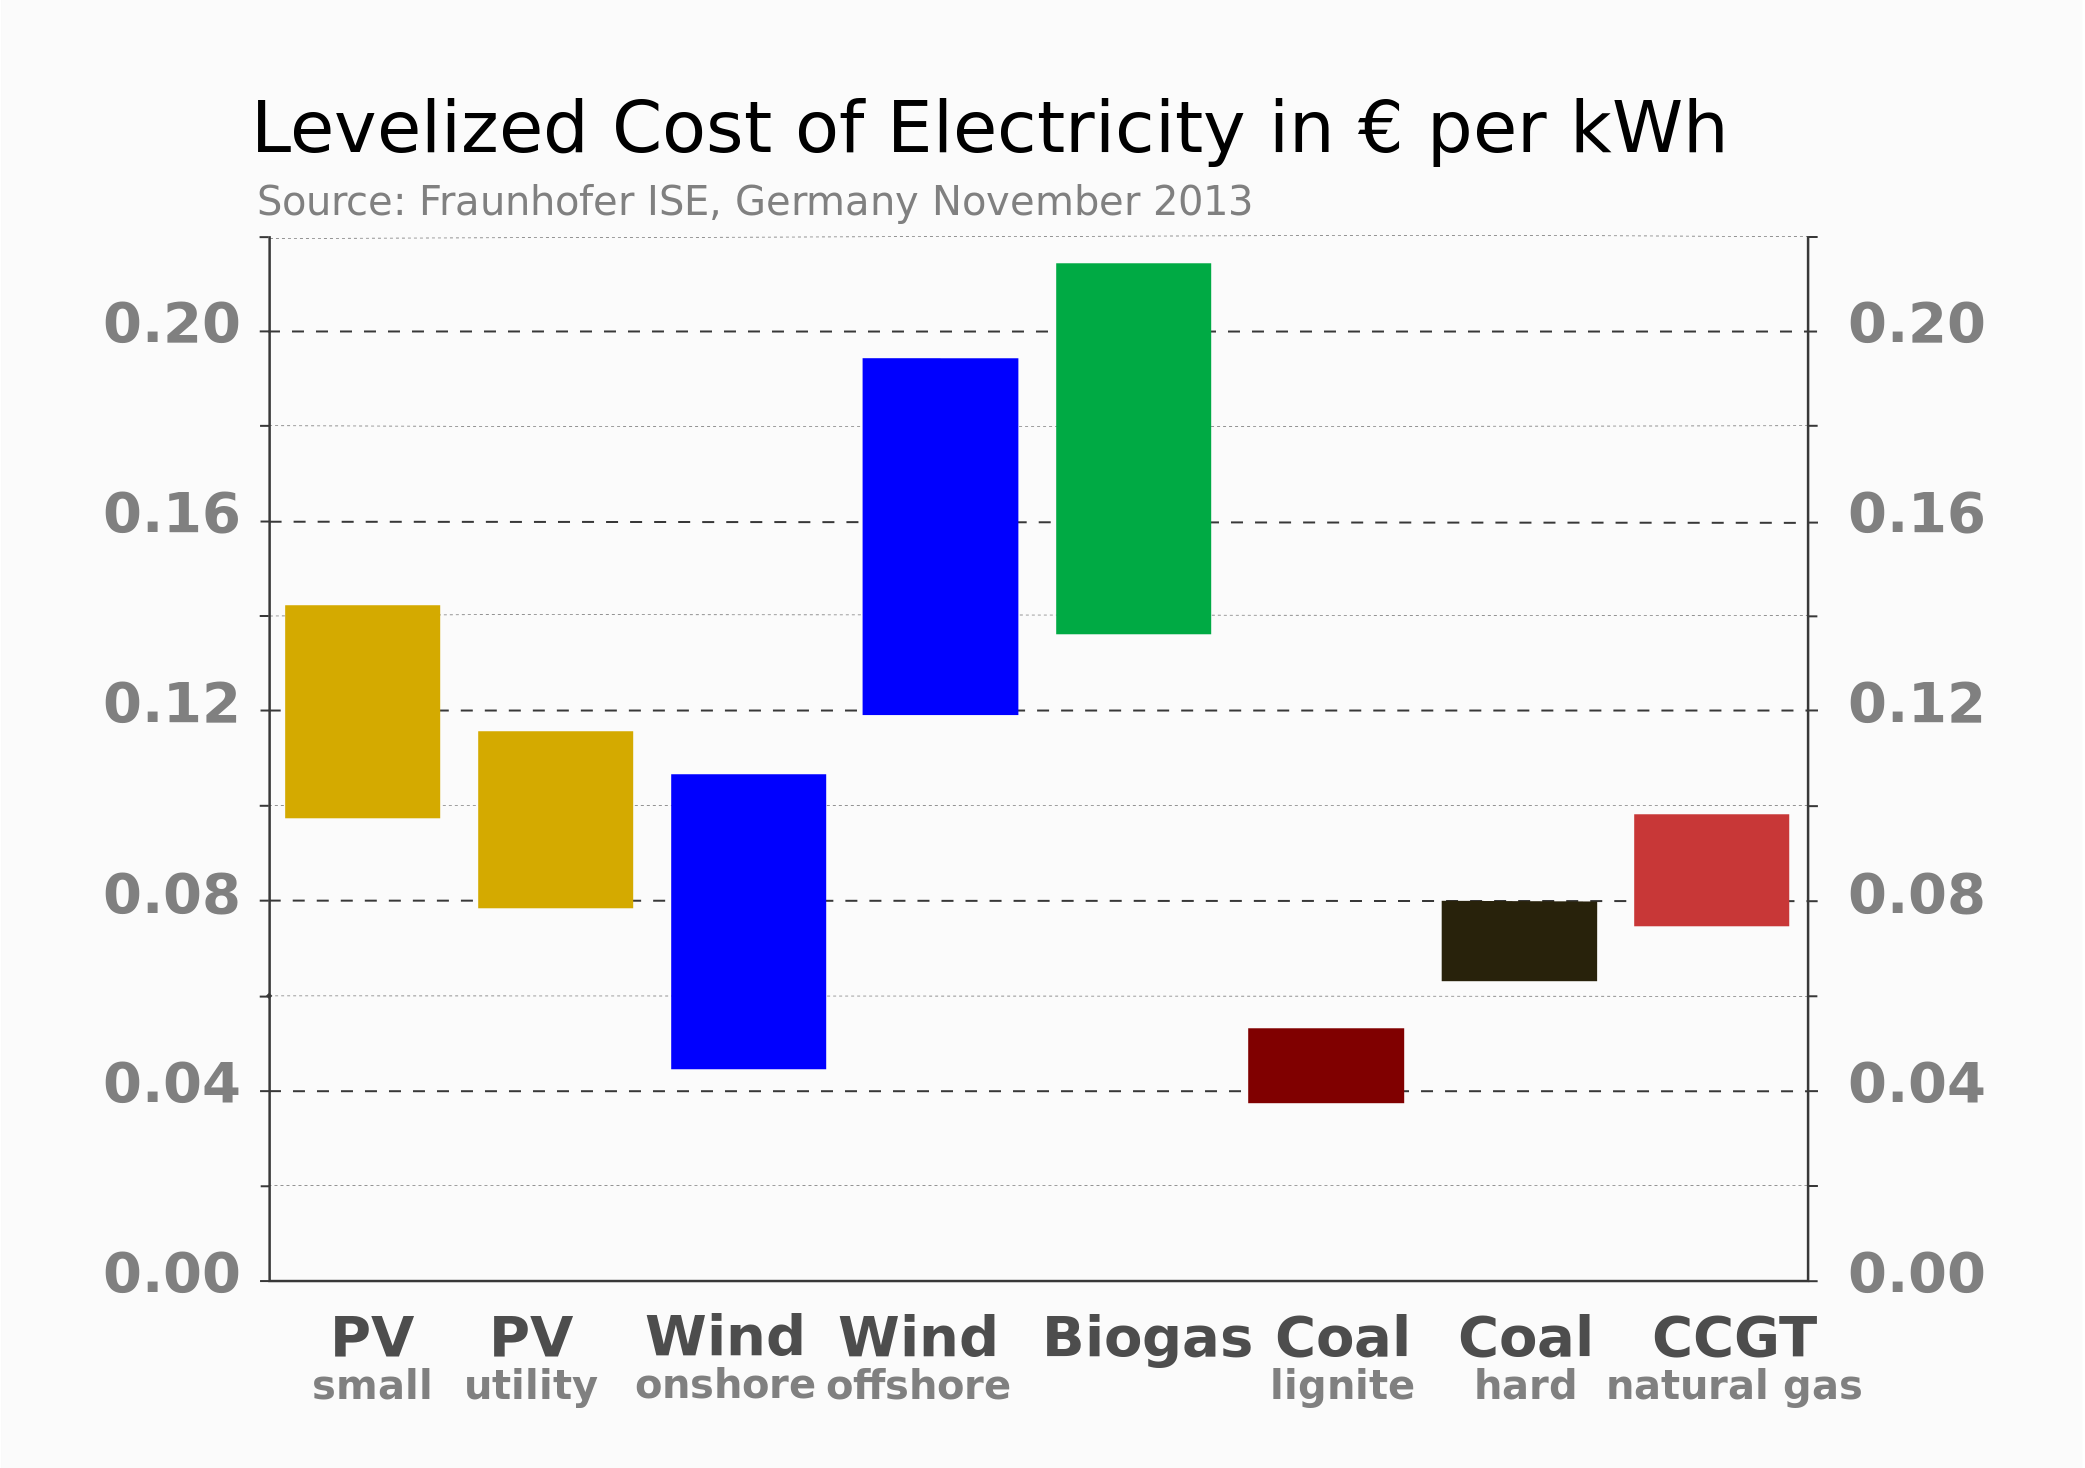
\includegraphics[width=0.8\textwidth]{figures/LCOE.png}
    \caption[Levelised cost of electricity (LCOE) of renewable energy technologies and conventional power plants at locations in Germany in 2013.  Specific investments are taken into account with a minimum and maximum value for each technology.]{Levelised cost of electricity (LCOE) of renewable energy technologies and conventional power plants at locations in Germany in 2013.  Specific investments are taken into account with a minimum and maximum value for each technology. Figure reproduced with permission from Ref.~\citenum{LCOE}.}
  \label{LCOE}
\end{figure}

%However if solar power, in combination with proper energy transport, storage and secondary conversion into heat and fuels, could be made to be economically feasible; it is a realistic candidate for replacing fossil fuels as a major supply of global energy. 

Levelised cost of energy, or electricity, (LCOE) is a common way to assess how cost competitive renewable energy sources are with their non-renewable counterparts. LCOE allows for the measurement of the performance of different power generating technologies, which may have unequal lifetimes and differing capacities. The LCOE is calculated by summing all costs incurred during the lifetime of the technology and dividing this value by the units of energy produced during the lifetime, with units of energy expressed as dollars per kilowatt hour (\$/kWhr) \cite{LCOE2}. This measure is also used as the key selling point for a number of commercial solar cell manufacturers such as First Solar Inc., who market their product as being able to generate electricity at an average of \$0.63 per Watt as stated in their 2013  Annual Report \cite{first_solar}. Using the LCOE, comparisons of grid competitiveness for renewable energy sources can be made \cite{LCOE2}. Fig.~\ref{LCOE} shows the LCOE of renewable energy technologies and conventional power plants at locations in Germany in 2013, enabling an assessment of the cost-competitiveness of PV power generation at this location, accounting for, for example, typical solar irradiation at the given locations \cite{LCOE}. Fig.~\ref{LCOE} shows that both small-scale and large-scale utility solar power were not cost competitive with the cheapest non-renewable resources. In the next section, both commercial solar cell technologies that are currently available and emerging technologies are discussed to understand why solar power is currently not cost competitive, and how emerging technologies may be able to improve the status quo for global solar power generation.

%Germany is an example of a country making considerable efforts to increase the percentage of their energy supplied by solar power. 
%On the 9\textsuperscript{th} of June 2014 Germany even generated over 50\% of its electricity demand from solar for the first time \cite{Germany_guardian_news}. Although on average the country is not able to produce such a large portion from solar power, with solar-generated power providing approximately 7.5\% of net electricity consumption in 2015 \cite{Germany_PV}. 
%To facilitate the growth of the solar power capacity in Germany a number of schemes and financial incentives to encourage investment were introduced, such as feed-in tariffs (FiTs).

%\begin{figure}[h!]
%  \centering
%    \includegraphics[width=0.65\textwidth]{figures/global_energy.png}
%    \caption{Illustration of power available annually from various renewable energy resources, annual world energy consumption and total reserves of various non-renewable energy resources. Figure taken from reference \citenum{global_energy_fig}.}
%  \label{global_energy}
%\end{figure}

%\begin{figure}[h!]
%  \centering
%    \includegraphics[width=0.65\textwidth]{figures/BIPV.jpg}
%    \caption{A building integrated photovoltaics (BIPV) project fitted in the United States by BISEM-USA \cite{BIPV}.}
%  \label{BIPV}
%\end{figure}


\subsection{Current commercial solar cell technologies and limitations}\label{current_tech}
It was first observed in 1839 by Edmond Becquerel that sunlight could be used to generate electricity. Becquerel discovered that if  silver chloride was placed in an acidic solution, connected to platinum electrodes and exposed to sunlight, an electric current flowed. However, the effect was small and poorly understood before Albert Einstein's discovery of the photoelectric effect and explanation of the phenomena by the quantum nature of light in 1904 \cite{PV_history1}. Even then, it was not until the development of semiconductor technology during the silicon revolution of the 1950's that solar cells capable of generating significant amounts of electricity were fabricated.

The first silicon solar cell was created in 1954 in the Bell Laboratories with cells achieving efficiencies of 6\%. 
Originally solar cells were developed for extraterrestrial energy generation, such as the 108 solar cells used to supply energy to the Vanguard satellite in 1958 \cite{PV_history1}. The first oil crisis in 1973, however, highlighted the dependency of many economies on fossil fuels and the need to address the security of energy supply. 
%in particular for Japan and West Germany which had few of their own resources. 
As a consequence, solar cell research was no longer limited to only high-cost crystalline devices for extraterrestrial applications, but also into creating cheaper, commercial, thin-film solar cell technologies using absorber materials such as amorphous silicon, cadmium telluride (CdTe) and copper indium diselenide (CIGS) \cite{PV_history2}.

\begin{figure}[h!]
  \centering
    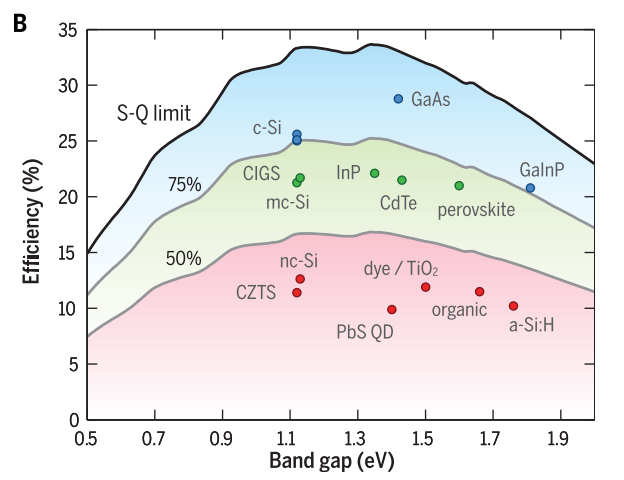
\includegraphics[width=0.75\textwidth]{figures/SQ_new.png}
    \caption[Theoretical Shockley-Queisser detailed-balance efficiency limit as a function of optical band gap (highest black line) for AM1.5 solar spectrum. The record efficiencies for different materials are plotted for the corresponding band gaps, where materials below the lower two grey lines are achieving conversion efficiencies less than 75\% and 50\% of their theoretical efficiency limit respectively.]{Theoretical Shockley-Queisser detailed-balance efficiency limit \cite{SQ_1961} as a function of band gap (highest black line) for AM1.5 solar spectrum. The record efficiencies for different materials are plotted for the corresponding band gaps, where materials below the lower two grey lines are achieving conversion efficiencies less than 75\% and 50\% of their theoretical efficiency limit respectively. Figure reproduced with permission from Ref.~\citenum{newPVrev}.}
  \label{SQ}
\end{figure}

Crystalline silicon is still the dominant solar cell technology with mono- and poly-crystalline silicon photovoltaic cells comprising up to 90\% of all the solar cells produced in 2008  \cite{Si_rev}. Silicon is the second most abundant element in the Earth's crust \cite{Si_abundance}. When considering this aspect alone, it seems to be a plausible material to use in large-scale solar power generation. Over 60 years of development have seen device efficiencies increase from 6\% to 25\% for the highest quality research devices and 15-18\% for the more common industrial cells \cite{Si_rev}. As can be seen from Fig. \ref{SQ}, the best performing silicon devices are now very close to achieving conversion efficiencies close to their theoretical limit, as predicted by the Shockley-Quiesser limit \cite{SQ_1961} for the optical band gap of the absorber. The fall in manufacturing costs is even more dramatic, more than halving between 2008 and 2013 and being a hundred times lower than they were in 1977, as shown in Fig.~\ref{Si_cost}. This development was largely aided by progress in semiconductor technology driven by the silicon chip industry, with the solar industry benefiting from advances in silicon manufacturing processes and even making use of waste silicon produced that was not of a high enough grade for silicon chips \cite{PV_history1}. Although the development of silicon-based technologies has clearly revolutionised the modern computer, the optical properties of silicon do not make it ideal for use as a solar absorber material in a photovoltaic device and despite the dramatic reduction in manufacturing costs, the technology is still not able to be cost-competitive with fossil-fuel power generation, as was shown in Fig.~\ref{LCOE}.

\begin{figure}[h!]
  \centering
    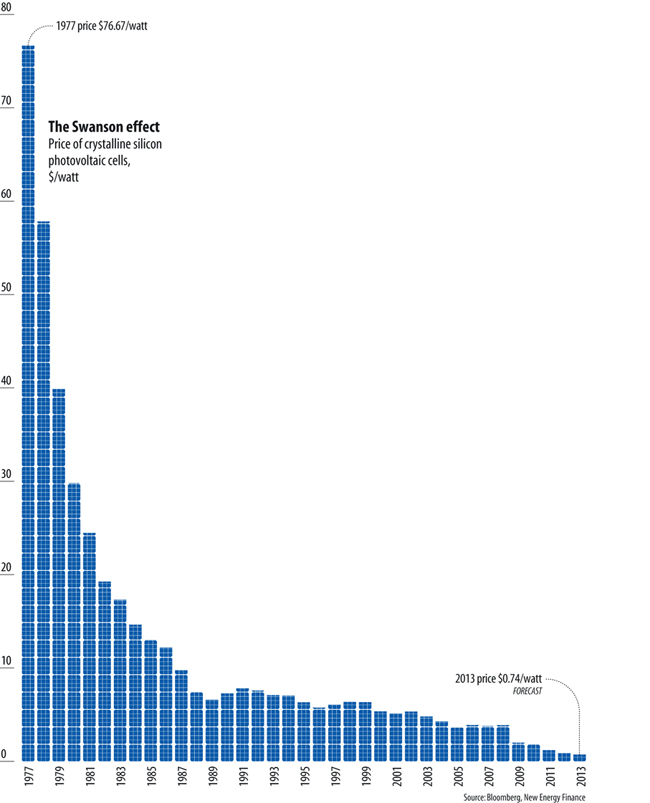
\includegraphics[width=0.8\textwidth]{figures/Si_cost.jpg}
    \caption[Average cost of solar panels composed of a crystalline silicon absorber layer.]{Average cost of solar panels composed of a crystalline silicon absorber layer. Figure reproduced with permission from Ref.~\citenum{PV_chart}.}
  \label{Si_cost}
\end{figure}

The primary issue with silicon is that its optical band gap of 1.1 eV is indirect. The importance of the electronic band gap in relation to PV performance will be discussed further in section \ref{PV_properties}. For now, it is just noted that the key consequence of the indirect nature of the band gap of silicon is that it is not a very strong absorber of sunlight (compared to for instance newer, thin-film technologies which are discussed next), resulting in a low optical absorption coefficient  compared to these newer technologies. To absorb the same amount of sunlight with a silicon solar cell requires a thicker layer of the material than in thin-film technologies. PV devices are very sensitive to defects and impurities. This point is discussed further in section \ref{defects_impact}, but the consequence for a thick layer of silicon is that very high quality, non-defective material is necessary to enable charge carrier collection before electron-hole recombination occurs, which results in high manufacturing costs. The devices are made from flat sheets of crystalline or multi-crystalline silicon called wafers that consist of very high quality silicon (99.999999\% pure) 
\cite{sus_book_5}.
The production processes of silicon wafers have been thoroughly optimised, but are still very energy-intensive, time-consuming and complex \cite{emerging_pv}.
%and this is reflected by the position of this type of technology on the plot of efficiency versus cost shown in figure \ref{PV_generations}. 
Despite decades of development, commercial silicon solar panels are still too expensive to compete with fossil-fuel based power sources \cite{FE_PV_rev1_5}. 

\subsubsection{Beyond silicon}

The `holy grail' of research into new materials for PV devices would be to find materials that are strong absorbers of sunlight, could be produced cost-effectively and composed of materials that are abundant enough for large-scale fabrication of the devices. 
%Such a drive has resulted in the development of what are considered three generations of solar energy technology. These are shown in figure \ref{PV_generations}, where highly efficient crystalline silicon devices with high associated manufacturing costs are considered the first generation of solar cell technology.
Thin-film solar cell devices make use of materials that are much more optically thick than silicon (i.e. stronger absorbers of sunlight with direct optical band gaps and higher optical absorption coefficients), which require less material to absorb the same amount of sunlight. %Figure \ref{thin_films} shows a comparison between the thickness of the aborber layer in some commercial second-generation PV devices to that of first-generation silicon wafers. 
The consequence of the reduction in the thickness of the absorber layer is that it is then less important for the material to be of as high-quality as in crystalline silicon devices, which enables the use of low-cost and low-energy fabrication methods \cite{emerging_pv}. Many thin-film technologies are also light-weight and flexible, allowing for more options for innovative deployment of the modules, such as building integrated photovoltaics (BIPV) and portable devices.

%Typically the efficiencies of second-generation solar cells are less than that of the best performing first-generation devices. 
Examples of commercial thin-film technologies include CIGS (Cu(In,Ga)(S,Se)$_2$) and CdTe. 
In the case of thin-film CuInSe$_2$ devices, it has even been found that the `lower quality' poly-crystalline material has a higher performance than its single crystal counterpart \cite{CIS1_3, CIS1_4}. Theoretical studies of the electronic properties of the grain boundaries in CuInSe$_2$ have provided an explanation for this unusual observation based on beneficial band offsets at the grain boundaries \cite{CIS1, CIS2}. This effect is a special case for this material, but it embodies the general ideology of thin-film technology well - namely to produce materials able to convert sunlight into electricity as efficiently as possible, with the simplest synthesis techniques possible.
Other innovations in PV technology include the use of multiple energy threshold devices to overcome the Shockley-Quiesser limit \cite{SQ_1961} for a single band gap solar cell, such as in tandem solar cells where semiconductor p-n junctions of increasing band gap are placed on top of each other in order to capture more of the solar spectrum. Typically these more complicated device architectures result in higher fabrication costs. Research efforts are therefore largely focused on reducing the fabrication cost of multi-junction devices \cite{3rd_gen}.

%\begin{figure}[h!]
%  \centering
%    \includegraphics[width=0.9\textwidth]{figures/thin_films2.png}
%    \caption{Typical structures of a commercial wafer-based PV device (first left) and commercial thin-film photovoltaic devices, as well as a CZTS thin-film device (right). The absorber layers are labelled in white and thickness is shown to scale. Figure adapted from reference \citenum{pathways}.}
%  \label{thin_films}
%\end{figure}

Current mainstream solar cell technologies, such as Si wafers and thin-film CdTe and CIGS solar cells, are unlikely to be able to provide solar electricity at the terawatt scale due to the scarcity of Te and In and the relatively long energy payback time for crystalline Si due to the cost and energy intensive fabrication of Si wafers \cite{CZTS_vs_MAPI}. 
Models have quantified such statements with a predicted In-constrained growth potential of power generation from CIGS PV technology of ~20 GW per year in 2020 due to competing applications of In, such as in liquid crystal displays \cite{culprit_5_3}.
To significantly increase the contribution of solar power to the global power supply, it is therefore necessary to develop more economically viable earth-abundant materials for sustainable PV electricity generation. Furthermore, there must be considerable technological breakthroughs that would enable low-cost manufacturing of high-efficiency devices with enough of a cost benefit to outweigh the initial cost outlay in optimising the manufacturing process of the whole device as has been done for silicon over the past 60 years. For this purpose, there is a drive for solar absorber materials with more optimal properties, such as a direct and sunlight matched band gap (as in thin-film technologies such as CdTe and CIGS), but also for materials that are composed of only earth-abundant components.\\

%** Add data on elemental abundance here and comment on in text?? **

\subsection{Examples of emerging metal sulfide solar absorbers}

The magnitude of the optical band gap is the most fundamental, necessary property of a semiconductor in order to have the potential to produce a high-efficiency solar cell device. Other important material properties for the absorber material in a PV device are discussed in section \ref{PV_properties}, but for now it is just noted that to maximise the energy harvesting potential of the PV device, a band gap for the absorber that is direct in nature and closely matched to the major component of the solar spectrum is desirable, this corresponds to a range of approximately 1.0 to 1.7 eV \cite{PV_E_range}. The optical band gap is the most fundamental and obvious screening criteria to use when selecting new candidate absorber materials for photovoltaic devices. The band structure of semiconductors will be discussed further in section \ref{BandTheorySection}, but for now it will just be noted that metal tellurides, selenides and sulfides typically have band gaps within the optimal energy range for PV applications due to the chalcogen p-orbital (which is usually the dominant component of the valence band maximum) being higher in energy than, for instance, the oxygen p-orbitals in metal oxides, which typically have band gaps that are too wide for PV applications. Of metal tellurides, selenides and sulfides, sulfur stands out in the interests of abundance and minimising toxicity.

SnS is an example of a non-toxic and earth-abundant metal sulfide that has received research interest for solar cell applications. SnS has a direct band gap within the optimal range for sunlight absorption of between 1.30 eV \cite{Lee_thesis_59} and 1.43 eV \cite{Lee_thesis_60}. However, record power conversion efficiencies (PCE) of PV devices are at around just 4\% \cite{SnS_record}. The low-performance of SnS devices has been attributed to several factors including the defect physics \cite{Lee_SnS_defects}, non-optimal band alignment in devices \cite{Lee_SnS_band} and phase impurity \cite{Lee_SnS_phases} of the material.

Kesterite-structured {\CZTS} (CZTS) has also received a large amount of research interest for PV applications, also due to the highly desirable earth-abundance and non-toxicity of its constituent elements, along with promising optical properties. The band gap of CZTS has been predicted \cite{CZTS_bandgap_theory} and measured \cite{CZTS_bandgap_exp} to be direct with a magnitude of 1.5 eV. 
The record device efficiencies are more than double that of SnS-based solar cells. However, CZTS solar cells still fall far short of their theoretical maximum PCE of 28\% predicted from the Shockley-Quiesser limit based on the optical band gap and have considerably lower performance than CdTe and CIGS solar cells as shown in Fig.~\ref{SQ}. The current confirmed record device efficiency of a sulfide-selenide alloy is 12.6\% \cite{Mitzi2017_rev_21}, while that of the pure sulfide material lags even further behind at behind at 9.1\% \cite{CZTS_record}. A large component of this work seeks to investigate possible origins of the performance deficit of CZTS solar cells. The other major component of this work looks to identify photoactive ferroelectric (or `photoferroic') materials so that alternative routes to high-efficiency solar cells may be explored by exploiting novel PV phenomena observed in ferroelectric materials. This is discussed in more detail in section \ref{ferroPVsection}. 


\section{The role of computational modelling in material design and optimisation}
The discovery of new functional materials by experimental methods is largely hindered by high costs and the time-consuming optimisation of synthesis procedures \cite{high_tp}.
However, with the rapid increase in computational processing power and the availability of large-scale supercomputers, we are entering a very exciting era in computational materials design \cite{WMD_material_design_review}. Furthermore, electronic structure theory has advanced to a level where it is possible to obtain good quantitative agreement with experiment without using adjustable parameters fit to experiment, i.e. from first principles. The only inputs into these calculations are electronic mass, electronic charge, atomic numbers and masses of the constituent atoms in the material. From this, it is possible to obtain to fairly high accuracy the structure, lattice constants, charge densities and various electronic, magnetic, optical and transport properties \cite{RichardMartin_Ch1}. Therefore theory and simulation of materials has reached a point of possessing predictive power for material properties relevant for various applications, completely independent of experimental measurement.

There are two main contributions that computational simulations could make towards the technological breakthroughs needed for economically-viable, large-scale solar energy generation. Firstly, by predicting relevant properties of materials that are not currently utilised in solar cells and screening for certain desirable properties, material simulations are able to aid in the discovery of new materials that may be capable of out-performing current solar cell technologies. Such an approach allows for a less time-consuming screening of potential new materials for a given application before attempting to prepare just the most promising candidates in the laboratory. Experimental validation of predicted properties, however, is always an important follow up to account for additional features of the physical system not initially accounted for in the model. In the case of candidate solar absorbers, for example, the optical properties are often initially predicted for the perfect bulk crystal. In reality materials contain various types of defects. Methods exist to model different forms of defects in a crystalline system, some of which are discussed later in this work. However, this typically quite complex and idiosyncratic feature of the system is often not considered initially, largely due to the vast range of possible defect features in a material. The defect physics of a material is a prime example of an area in which knowledge and understanding is developed symbiotically between works from experiment and theory. Secondly, material simulations are able to provide valuable, atomistic insight on scales that cannot be probed experimentally to improve fundamental understanding of known photovoltaic materials, which may enable improvements in existing solar cell technologies. Defect physics is again a prime example of this. Theory can probe on the atomic scale to aid in the interpretation of experimental data obtained from a variety of different measurements.

In this work, materials modelling techniques are developed and applied to make both types of contribution to the field. A model is developed to improve current atomic-scale understanding of the candidate earth-abundant, non-toxic solar absorber material {\CZTS} (CZTS) and to provide a tool for assessing possible origins of the under-performance of this particular solar cell technology. This is the subject of \autoref{chap:CZTS}. Materials modelling is also used to predict the relevant properties of candidate photoferroic absorbers that are not currently utilised in solar cell technologies to identify those that are most likely to be worthy of further study. In \autoref{chap:screening}, the screening criteria and methodologies used in this study for identifying candidate photoferroic absorbers are discussed and some relevant calculated material properties for the candidates are presented. In \autoref{chap:insights}, the use of material simulations and theoretical insights to assess the likely performance of a material in a solar cell device is discussed further. In particular, knowledge gained from previous studies on more mature PV technologies is drawn upon when examining the potential of the candidate photoferroic materials for solar cell applications.

\section{Format of thesis}
The following thesis is in the `alternative format' which is a thesis incorporating academic papers that are published, accepted, submitted, or written as if for publication. All papers included in the thesis are labelled as publications and begin with a statement of authorship. All papers included in this thesis are first-author works, but contributions to the works from co-authors are indicated in the statement of authorship. The supplemental material for all publications are included as appendices.



\chapter{Theoretical background}                                                        

\section{Models of perfect, periodic solids}\label{crystal_models}
%Refer to: pg 28 29 35 \cite{thin_film_Boer}\\
To relate the properties observed for a material to its underlying atomic and electronic structure, and also to predict properties that have not yet been measured, it is necessary to have a suitable model for the material. Theoretical models of crystalline solids are based around the existence of translational symmetry in a crystal lattice such that the lattice can be constructed by periodically repeating a unit cell of atoms. The Bravais lattice specifies the periodic array in which the repeated units of the crystal are arranged. A crystal lattice can therefore be described by its underlying Bravais lattice and the arrangement of atoms, ions or molecules within a particular unit cell, i.e. the basis \cite{AshcroftMermin2}. This principle is also used in electronic calculations of solid state systems through the implementation of periodic boundary conditions to simulate an infinite, bulk system using only a finite unit cell. Methodologies used in electronic structure calculations will be discussed further in section \ref{elec_struc}.
 
Another important concept in the theoretical modelling of periodic structures is reciprocal space and the reciprocal lattice. 
Converting to reciprocal space enables the description of periodic features with a longer-range periodicity than the unit cell in real space, such as the motion of electrons in a crystal and phonons.
%In the same way that any quantity that varies with time can be described as a sum of Fourier components in the frequency domain; 
The spatial properties of a crystal can be described as a sum of components in Fourier space, otherwise known as reciprocal space or \textit{k}-space. A wave in real space can be represented by a point in reciprocal space. The reciprocal lattice of a perfect single crystal is an infinite periodic 3D array of points whose spacings are inversely proportional to the distances between the planes in the lattice in real space. Vectors in real space have dimensions of length, whereas vectors in reciprocal space have dimensions of inverse length. This can be compared directly to the wavevector $ \left(k  = \frac{2\pi}{\lambda} \right)$ of an excitation such as a phonon or a moving electron and multiplication of each coordinate of the reciprocal lattice by $\hbar$ converts reciprocal space into momentum space, as for a quantised wave $\mathbf{p} = \hbar \mathbf{k}$ \cite{Blakemore1}. 

\begin{figure}[h!]
  \centering
    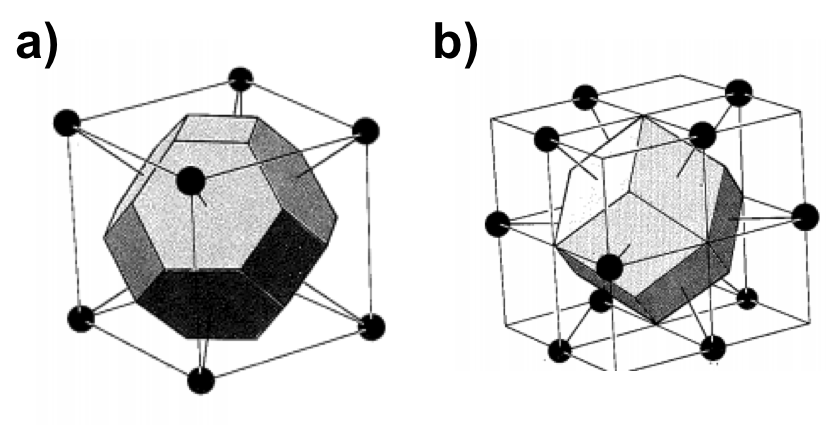
\includegraphics[width=0.5\textwidth]{figures/Wigner-Seitz.png}
    \caption[The Wigner-Seitz cell for the body-centred cubic Bravais lattice where there is a lattice point at its centre and on each vertex (a) and the face-centred cubic Bravais lattice (b).]{The Wigner-Seitz cell for the body-centred cubic Bravais lattice where there is a lattice point at its centre and on each vertex (a) and the face-centred cubic Bravais lattice (b). 
    %The hexagonal faces bisect the lines joining the central point to the points on the vertices. The square faces bisect the lines joining the central point to the central points in each of the six neighbouring cubic cells. 
    Figure reproduced with permission from Ref.~\citenum{AshcroftMermin2}.}
  \label{Wigner-Seitz}
\end{figure}

The Wigner-Seitz primitive cell is the most common choice of primitive cell with the full symmetry of the Bravais lattice. It represents the region of space around a lattice point  that is closer to that point than to any other lattice point. For example, Fig.~\ref{Wigner-Seitz}a shows the truncated octahedron that is the Wigner-Seitz cell for a body-centred cubic (bcc) lattice \cite{AshcroftMermin2}.
The first Brillouin zone is the Wigner-Seitz primitive cell of the reciprocal lattice. The reciprocal of the bcc lattice is face-centred cubic (fcc), therefore the first Brillouin zone of the bcc lattice is the fcc Wigner-Seitz primitive cell as shown in Fig.~\ref{Wigner-Seitz}b \cite{AshcroftMermin3}. As the full symmetry of the reciprocal lattice is contained within the first Brillouin zone, it is only necessary to sample \textit{k}-points within this single unit cell of the reciprocal lattice when calculating the electronic ground state of a periodic structure.



\section{Electrons in periodic solids}\label{BandTheorySection}

%** + cross-ref Prasad Ch4 **

%Refer to: pg 18 \cite{fund_semi}, pg 105 112 128 131 137 \cite{thin_film_Boer}, pg 111 + 119 \cite{phys_semicond}\\
%** Highlight link to PV and indication of PV performance from band structure + check against Nelson CH3\\
%The band theory of solids provides a means to explain the difference in the electrical conductivity of conductors, semiconductors and insulators. 
Electrons bound to an atom in atomic orbitals have a number of possible discrete energy levels. When a pair of atoms are brought together to form a molecule, the atomic orbitals combine to form pairs of molecular orbitals arranged with energy levels slightly higher and slightly lower in energy than the original energy levels, referred to as antibonding and bonding orbitals respectively. When a large number of atoms are brought together to form a solid the 
%it becomes impossible to assign individual electrons to individual atoms. Instead, the electrons are considered to be shared amongst the atomic nuclei. A consequence of this sharing would be a large number of electrons occupying the same energy state, which violates the Pauli Exclusion Principle. The 
original discrete energy levels are broadened into new energy levels that are so closely spaced that they are considered to be a quasi-continuous band of allowed energies. This is illustrated in Fig. \ref{band_Elevels}. 

\begin{figure}[h!]
  \centering
    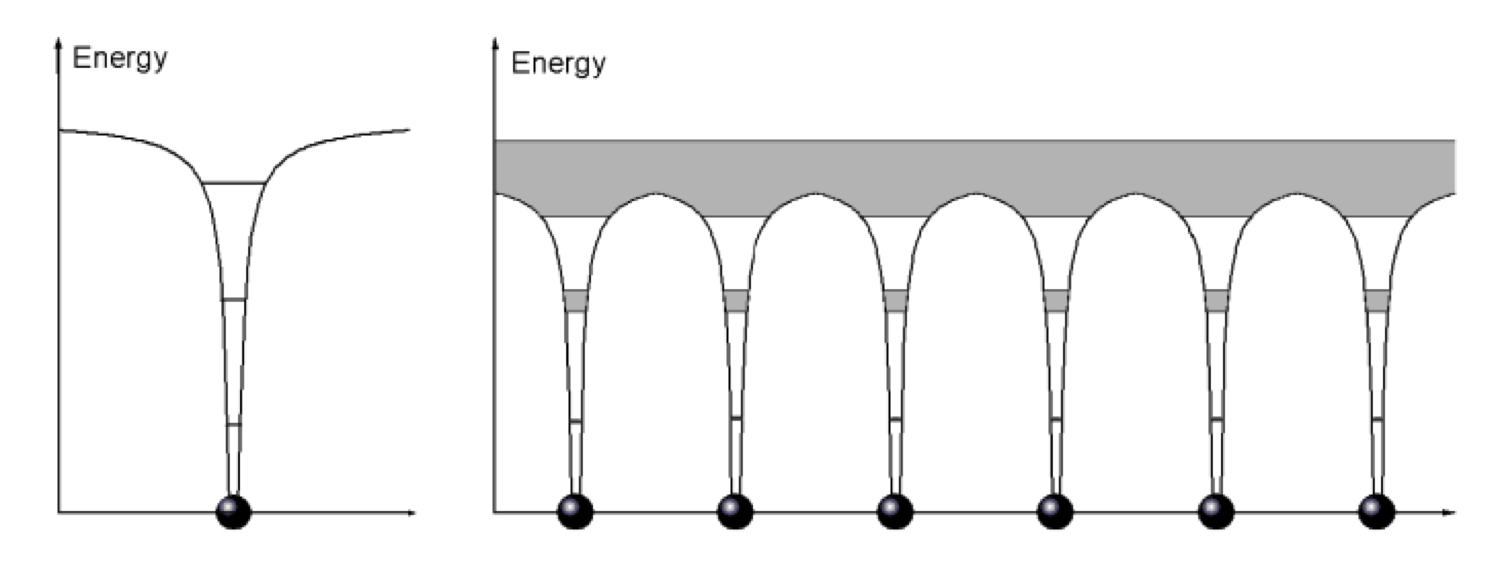
\includegraphics[width=0.7\textwidth]{figures/band_Elevels.png}
    \caption[Electron energy levels of a single atom (left) and the formation of a quasi-continuous band of allowed energies in a solid crystal when many atoms are brought close together (right).]{Electron energy levels of a single atom (left) and the formation of a quasi-continuous band of allowed energies in a solid crystal when many atoms are brought close together (right). Figure reproduced with permission from Ref.~\citenum{mat_prop1}.}
  \label{band_Elevels}
\end{figure}

The energy distribution of the bands depends upon the electronic properties of the constituent atoms of the crystal and the strength of the bonds between them. Bands are occupied if the original molecular orbitals were occupied. The highest-energy occupied band (containing the valence electrons) is the valence band (VB). The lowest unoccupied band is the conduction band (CB). If the VB is only partially filled or if it overlaps in energy with the CB, then the solid is a metal. The availability of empty states at energies close to that of the occupied states facilitates easy scattering of valence electrons into neighbouring states, thereby allowing for the transport of heat and charge. Hence metals conduct both heat and electric current. In a semiconductor or insulator, the VB is completely full and separated from the next unoccupied CB by an energy gap called the optical band gap, E$_g$ \cite{Nelson3}. In the simplest model, the CB is separated from the VB by a constant E$_g$. This is called the flat band model and is often shown in schematics of junctions for PV device architectures, which will be discussed in section \ref{junctions}. In real structures, the band architecture is more complicated than this simple model, like the band structures shown later in Fig.~\ref{Si_and_GaAs} \cite{Tilley}.


\subsection{Bloch's theorem}

To understand the behaviour of electrons in solids, Bloch's theorem is invoked to describe the wave function of a particle in a periodic potential. The electron is considered as a wave propagating in a periodic structure, i.e. the periodic crystal lattice \cite{small_semiconductor1}. The Schr{\"o}dinger equation (SE) must be solved to determine the energy of electrons in a solid. 
The energy of a single, independent electron in a perfect crystal is described by the one-electron SE, shown in Eq.~\ref{single_SE}. The first term in Eq.~\ref{single_SE} is the kinetic energy of the electron, V(\textbf{r}) is the effective periodic potential energy experienced by the electron in the crystal, $\psi$ is the electron wavefunction and $\epsilon$ is the eigenenergy of the electron.
\begin{equation} \label{single_SE}
\left[ \left(-\frac{\hbar^2}{2m}\right)\nabla^2 + V(\mathbf{r})\right]\psi = \epsilon \psi 
\end{equation}
For a solid, the infinite array of atomic potentials making up the crystal must be accounted for, as opposed to just the few associated with a molecule. For this purpose the periodicity of crystalline solids, outlined in section \ref{crystal_models}, is exploited to determine the probability distribution of electrons in an infinite solid \cite{Nelson3}. 
The spatial dependence of the potential experienced by an outer electron in a crystal for multi-electron systems was considered by Felix Bloch. Bloch determined that the total potential is the sum of two parts. Firstly, the electrostatic potential due to the array of atomic cores. For a perfect lattice this should have the translational periodicity of the lattice. Secondly, the potential due to all other electrons. Bloch assumed that the charge density would have the same long-term average value in every unit cell of the crystal and therefore would be periodic \cite{fund_semi}.
The periodicity of the crystal lattice means that the probability distribution of the electrons must also be periodic, with no preference for an electron to occupy a particular site within one unit cell than any others. Furthermore, as the lattice is infinite, electrons in a periodic solid should form delocalised states which extend throughout the crystal in a similar manner to an electron in free space.

%** Add figure showing Bloch function?? (like group vs phase velocity??) + c.f. other theses – use Richard Martin Fig 4.11?? **

Bloch's theorem states that the wavefunction which satisfies Eq.~\ref{single_SE}, subject to a periodic potential, should be of the form shown in Eq. \ref{bloch}. This Bloch function is a product of a function $U_{i\mathbf{k}}(\mathbf{r})$, which possesses the periodicity of the lattice, and a plane wave part, where \textbf{k} is the wavevector of an electron propagating in the crystal bands i \cite{Nelson3}.
\begin{equation} \label{bloch}
\phi_k(\mathbf{r}) = U_{i\mathbf{k}}(\mathbf{r}) e^{i\mathbf{k \cdot r}} 
\end{equation}
\begin{equation} \label{bloch_sum}
\psi_k(\mathbf{r}) = \sum_k A_k \phi_k(\mathbf{r}) = \sum_k A_{i\mathbf{k}}U_{i\mathbf{k}}(\mathbf{r}) e^{i\mathbf{k \cdot r}} 
\end{equation}
Due to the translational symmetry of a crystal lattice, an eigenfunction of the one-electron SE can be expressed as a sum of Bloch functions such as that shown in Eq. \ref{bloch}, to give Eq. \ref{bloch_sum}. 


\subsection{Electronic band structure}

\begin{figure}[h!]
  \centering
    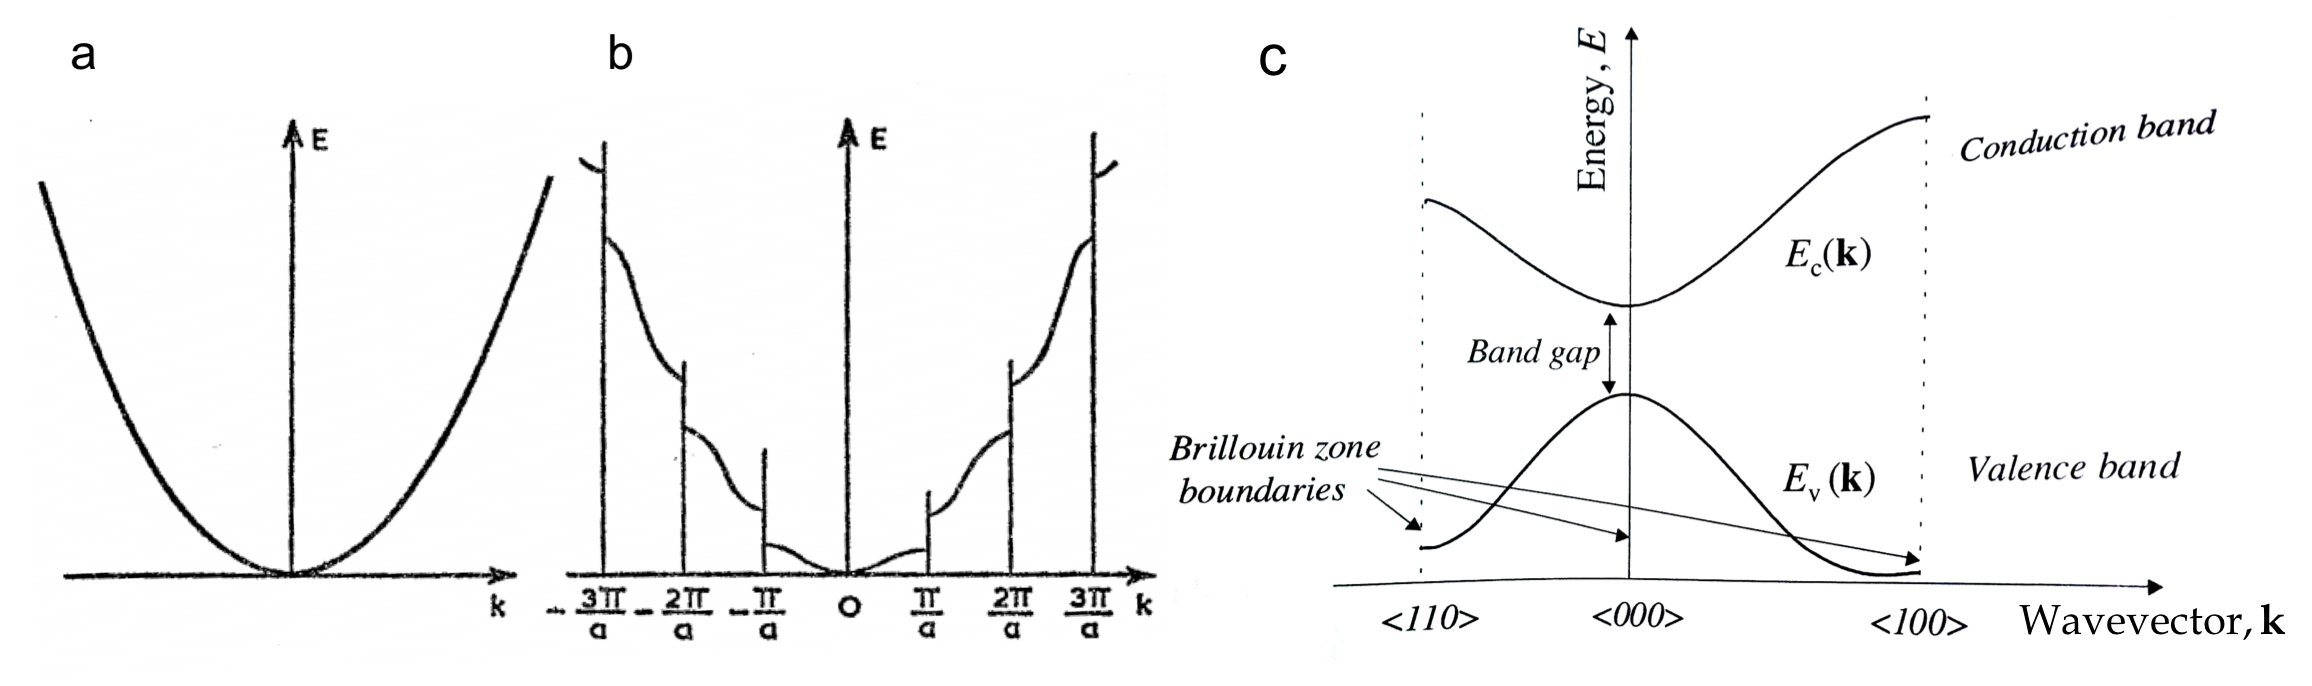
\includegraphics[width=0.95\textwidth]{figures/bs1_2.png}
    \caption[Energy-wave vector diagrams: (a) the free electron parabola, (b) modification due to a periodic crystal lattice.]{Energy-wave vector diagrams: (a) the free electron parabola, (b) modification due to a periodic crystal lattice. Figure a and b reproduced with permission from Ref.~\citenum{small_semiconductor1}, figure c reproduced with permission from Ref.~\citenum{Nelson3}.}
  \label{bs1}
\end{figure}
The one-electron wavefunctions can be indexed by constants \textbf{k} and i \cite{fund_semi}. 
$U_{i\mathbf{k}}(\mathbf{r})$ and electron eigenenergies, $E(\mathbf{k})$, from Eq. \ref{single_SE} are found by solving the SE for each band i and for each \textbf{k} \cite{Nelson3}.
A plot of $E(\textbf{k})$ versus \textbf{k} is known as the energy dispersion relation or electronic band structure of the crystal \cite{fund_semi}.
The impact of a medium with a discrete structure, such as a crystal lattice, on the energy dispersion relation of a free electron can be seen by comparing Fig.~\ref{bs1}a to Fig.~\ref{bs1}b.
E(\textbf{k}) of a material is usually plotted against $|\textbf{k}|$ just for the most important directions in the crystal, such as that shown in Fig.~\ref{bs1}c. A periodic medium does not suppress the propagation of waves, as would be expected in disordered or amorphous structures, but introduces limiting frequencies and wavelengths for the propagation. 

The parabola for the free electron (shown in  Fig.~\ref{bs1}a) is modified in a periodic crystal by the introduction of discontinuities at values of $|\textbf{k}|$ corresponding to multiples of $\frac{\pi}{a}$, as shown by Fig. \ref{bs1}b \cite{small_semiconductor2}. The point $|\textbf{k}| = \frac{\pi}{a}$ is the Brillouin zone boundary. At these points the electron wavefunction is a standing wave and the gradient of E(\textbf{k}) disappears \cite{Nelson3}.
The lower limit of the wavelength is set by the lattice spacing, giving an upper limit of the wave vector, $|\textbf{k}|$, of $\frac{\pi}{a}$, where a is the spacing of the planes of atoms in the direction E(\textbf{k}) has been plotted.  The appearance of such energy gaps implies that electrons in a periodic crystal may only have kinetic energies corresponding to certain bands, whilst being free to propagate in the lattice \cite{small_semiconductor2}.
Due to the periodicity of the crystal lattice, $|\textbf{k}|$  that differ by multiples of $\frac{2\pi}{a}$ cannot be distinguished and E(\textbf{k}) repeats for $|\textbf{k}| > \frac{\pi}{a}$. 
%For most crystals, E(\textbf{k}) is identical to E(\textbf{-k}) since states with positive and negative $|\textbf{k}|$ are degenerate. 
Therefore all information for the energy dispersion relation, E(\textbf{k}) vs. $|\textbf{k}|$, of the material is contained in the range $0 < |\textbf{k}| < \frac{\pi}{a}$ and so only this region needs to be plotted, as in Fig \ref{bs1}c \cite{Nelson3}. 

A useful concept used to simplify the dynamics of an electron in a crystal lattice in the band theory of solids is that of the effective mass approximation. The effective mass is a convenient parameter determined from the curvature of the maxima and minima of the VB and CB respectively along particular paths in momentum space to account for the influence of a periodic lattice on a free carrier. This approximation enables an electron in a periodic crystal to be treated as though it were a free particle but with a different mass in calculations of charge transport \cite{small_semiconductor2}.
%$U_{i\textbf{k}}(\mathbf{r})$ depends weakly on \textbf{k}, but this dependence is neglected in the effective mass approximation \cite{Nelson3}.
The influence of the effective mass of charge carriers in a solar absorber material on the efficiency of a PV device composed of that material will be discussed in section \ref{PV_properties}.

%The concept of the energy band model of a solid emerges from considering the behaviour of electrons in a periodic crystal lattice, but cannot be understood in terms of classical physics alone. Instead, the electron must be considered in terms of wave-mechanical terms as a wave propagating in a periodic structure with diffraction and interference effects  \cite{small_semiconductor1}.
%In the band theory of solids, the energy of a single electron in a perfect crystal is described by the one-electron Schr{\"o}dinger equation, shown in equation \ref{single_SE}. The first term in equation \ref{single_SE} is the kinetic energy of the electron, V(\textbf{r}) is the effective non-zero periodic potential energy experienced by the electron in the crystal, $\psi$ is the electron wavefunction and  $\epsilon$ is the eigenenergy of the electron. In band theory, it is assumed that for any electron, everything else in the crystal can be represented by the effective potential energy, V(\textbf{r}) \cite{Blakemore2}.
%\begin{equation} \label{single_SE}
%\left[ \left(-\frac{\hbar^2}{2m}\right)\nabla^2 + V(\mathbf{r})\right]\psi = \epsilon \psi 
%\end{equation}
%The spatial dependence of the potential experienced by an outer electron in a crystal for multi-electron systems was considered by Felix Bloch. Bloch determined that the total potential is the sum of two parts. Firstly, the electrostatic potential due to the array of atomic cores. For a perfect lattice this should have the translational periodicity of the lattice. Secondly, the potential due to all other electrons. Bloch assumed that the charge density would have the same long-term average value in every unit cell of the crystal and therefore would be periodic. Bloch's theorem states that the wavefunction which satisfies equation \ref{single_SE} subject to a periodic potential should be of the form shown in equation \ref{bloch}, where $U_k(\mathbf{r})$ is some function 
%(depending on the value of the wavevector, \textbf{k}) that also has the complete periodicity of the lattice and \textbf{k} is confined to the first Brillouin zone \cite{Blakemore2}.
%\begin{equation} \label{bloch}
%\phi_k(\mathbf{r}) = U_k(\mathbf{r}) e^{i\mathbf{k \cdot r}} 
%\end{equation}
%\begin{equation} \label{bloch_sum}
%\psi_k(\mathbf{r}) = \sum_k A_k \phi_k(\mathbf{r}) = \sum_k A_kU_k(\mathbf{r}) e^{i\mathbf{k \cdot r}} 
%\end{equation}
%Due to the translational symmetry of a crystal lattice, an eigenfunction of the one-electron Schr{\"o}dinger equation can be expressed as a sum of Bloch functions such as that shown in equation \ref{bloch}, to give equation \ref{bloch_sum}. The one-electron wavefunctions therefore can be indexed by constants \textbf{k}, which are the wave vectors of the plane waves forming the `backbone' of the Bloch function. A plot of the electron eigenenergies from equation \ref{single_SE} versus \textbf{k} is known as the electronic band structure of the crystal \cite{fund_semi}.

%\subsection{Electrical conductivity of semiconductors}

The band theory of a semiconductor can also be used to understand the electrical conductivity of the material. At 0K electrons have no kinetic energy and therefore occupy the lowest energy states available, where the energy of the highest energy state filled is called the Fermi energy, E$_F$. However, at finite-temperatures electrons may have sufficient kinetic energy to access higher energy states above E$_F$, leaving behind some empty states below E$_F$. The distribution for electrons in thermal equilibrium at finite-temperatures is described by Fermi-Dirac statistics, where Eq.~\ref{fermi-dirac} gives the probability that an electronic state of energy E will be occupied at some temperature T, where k$_B$ is the Boltzmann constant \cite{Nelson3}.
\begin{equation}\label{fermi-dirac}
f(E) = \frac{1}{e^{(E-E_F)/k_BT}+1}
\end{equation}
In a semiconductor at 0K, the VB is fully occupied by electrons and the CB is completely unoccupied and so electrical conduction is not possible. However as temperature is increased it may become possible for electrons to access unoccupied states in the CB if they have sufficient energy to overcome the band gap, allowing for some electrical conduction. Typically, the band gap of an electrical insulator is too large for this to occur. It is also possible for the energy gap to be decreased by defects and doping \cite{Nelson3}, which will be mentioned in regards to the impact on PV performance in section \ref{defects_impact}. The band gap of a semiconductor, and in particular the magnitude of the band gap, is also an important property for the photovoltaic effect where electrons are optically excited across this energy gap by incident photons, which will be outlined in the next section.

%Values of effective mass in semiconductors usually vary between 0.01 and 1 times the mass of a free electron and it is determined by the curvature of the energy graph in \textit{k}-vector space \cite{small_semiconductor2}. The effective mass is a parameter that can influence the efficiency of a solar cell. The mobility of charge carriers is inversely proportional to the effective mass and the mobility of charge carriers in a PV material is important for efficient charge collection \cite{transport}.\\

%Each electron occupies a state of definite $\mathbf{k}$. Therefore, an infinite number of electrons within the solid would result in an infinite number of \textit{k}-points. At each \textit{k}-point, only a finite number of the available energy levels will be occupied. Therefore only a finite number of electrons need to be considered but at an infinite number of \textit{k}-points. In practise, all of these \textit{k}-points are not considered. 
%Electron wavefunctions will be almost identical for values of $\mathbf{k}$ that are sufficiently close, so the wavefunctions over a region of reciprocal space can be represented by considering the wavefunction at a single \textit{k}-point. It is therefore sufficient to consider the electronic states at a finite number of \textit{k}-points in order to determine the ground state energy of the solid. This approximation is illustrated in figure \ref{energy_dispersion}. Using Bloch's Theorem therefore has enabled the ground state energy to be determined by considering only the number of electrons in the unit cell at a finite number of \textit{k}-points, which are chosen to sample the Brillouin zone appropriately. The choice here is a balance between more \textit{k}-points for a more accurate representation of the Brillouin zone and fewer \textit{k}-points to reduce the computational expense of the calculation \cite{bloch-thesis}.

%\begin{figure}[h!]
%  \centering
%    \includegraphics[width=0.4\textwidth]{figures/energy_dispersion.png}
%    \caption{The energy dispersion relation for electrons moving in a crystal, illustrating how the function can be approximately represented by a finite number of \textit{k}-points, which form an equally-spaced mesh. Figure adapted from reference \citenum{vasp-slides}.}
%  \label{energy_dispersion}
%\end{figure}


\section{The photovoltaic effect}
A solar cell device converts incident solar energy directly into electrical energy. Solar energy can be described as either a spectrum of electromagnetic radiation, in the classical-wave theory of light, or as a flux of packets of energy (photons), in the quantum theory of light. Electrical energy is a flow of charge carriers able to do work in an external circuit \cite{spatial_resolved_book}. Voltage is generated in a solar cell device by the photovoltaic effect (PVE). The terms `solar cell' and `photovoltaic (PV) cell' are therefore often used interchangeably. The explanation for the PVE uses ideas from the quantum theory of light \cite{Nelson1}.

\begin{figure}[h!]
  \centering
    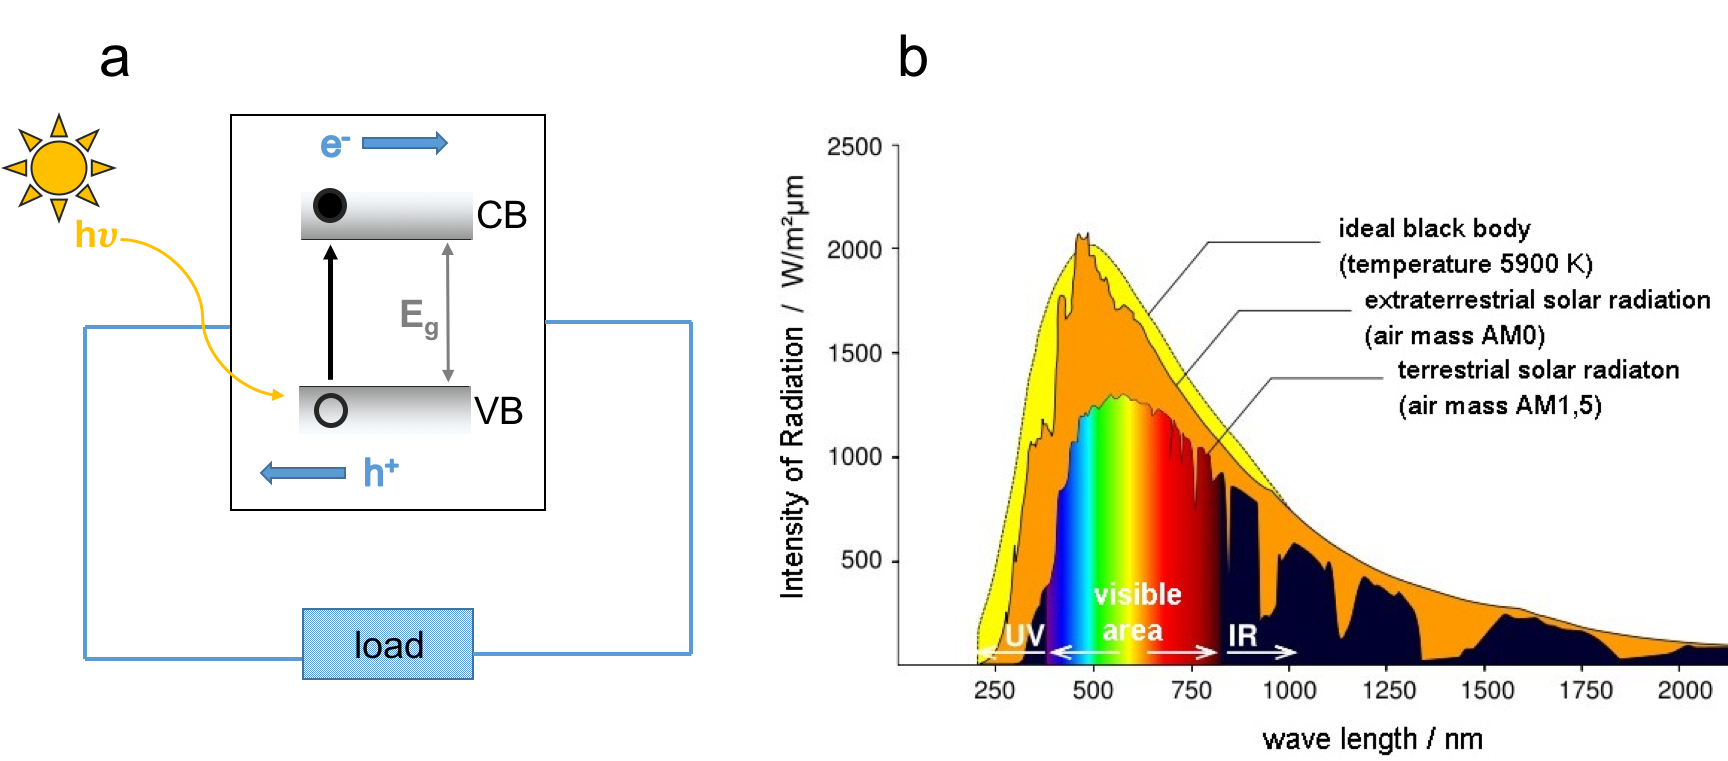
\includegraphics[width=0.95\textwidth]{figures/PV_schematic.png}
    \caption[Schematic of the photovoltaic effect: a semiconductor under illumination with some built-in electrical asymmetry to drive the separation of charge carriers to be fed into an external circuit and an external load to do electrical work (a). The AM1.5G solar spectrum, indicating the major component that is in the energy range of visible light (b).]{Schematic of the photovoltaic effect: a semiconductor under illumination with some built-in electrical asymmetry to drive the separation of charge carriers to be fed into an external circuit and an external load to do electrical work (a). The AM1.5G solar spectrum, indicating the major component that is in the energy range of visible light (b). Figure b reproduced with permission from Ref.~\citenum{PV_spectrum}.}
  \label{PV_schematic}
\end{figure}

Semiconducting materials can be used as the absorber layer in a PV device, the presence of an optical band gap, E$_g$, in the electronic structure of the material is vital for the PVE. In the case of a perfectly pure semiconductor, only photons with energies higher than the intrinsic E$_g$ can be absorbed to excite an electron from the VB into the CB to produce an electron-hole pair, as shown in Fig.~\ref{PV_schematic}a. In order for this process to be induced by sunlight, the magnitude of E$_g$ must be within the range of the photon energies that make up the solar spectrum, which is shown in Fig.~\ref{PV_schematic}b. E$_g$ of a semiconductor is also necessary for the electrons that have been optically excited to gain extra electrochemical potential energy, which provides the potential difference, or electromotive force, that will later drive electrons through a load in an external circuit to do electrical work. If electrons are instead promoted through a continuum of energy levels, as in a metal, excited electrons would quickly decay back to the ground state via intermediate energy levels, thus dissipating the potential energy gained. In the conventional PV effect, E$_g$ of the material sets the upper limit for the voltage that can be generated. The voltage at open circuit (when current is zero), V$_{OC}$, is the maximum possible potential difference across the terminals of the solar cell. However, in order for the cell to do any electrical work, both voltage and current (and hence power) must be non-zero when a load is connected in the external circuit \cite{Nelson3}.

In the absence of a driving force to separate the photoexcited electron and hole, the pair would quickly recombine and relax back to the ground state of the material with the emission of a photon of an energy equal to the energy of the electronic transition that has just occurred. In a PV device there is a `built-in' electrical asymmetry that provides an electric field to pull electrons away before they can relax and drive them towards electrical contacts to be fed into an external circuit. An electric field is effective for charge separation because it drives positively and negatively charged carriers in opposite directions \cite{Nelson5}. There are various ways to provide the electrical asymmetry, such as: through connecting a metal and a semiconductor to form a Schottky barrier junction and connecting a p-type semiconductor to an n-type semiconductor to form a p-n junction. These types of device architectures are outlined in the next section. In section \ref{ferroPVsection}, novel PV phenomena in bulk materials with internal electric fields, but without the need for such junctions, will be outlined and a search for candidate `photoferroic' materials is presented in \autoref{chap:screening}. The motivation of this investigation was to find materials where it may be possible to exploit the internal electric fields of polar crystals for enhanced local charge carrier separation.



\section{Solar cell junctions}\label{junctions}
As discussed in the previous section, an electrical asymmetry is vital for the PVE. A light absorber material must be connected to an external circuit by paths of different resistance for positive and negative charge carriers, i.e. for holes and electrons. This can be provided by spatial variation in the electronic environment, such as the junction between two electronically distinct materials.
An electrostatic field can be established by creating a junction with a gradient in the work function ($\Phi_W$), electron affinity (EA) or band gap ($E_g$), which are all labelled in Fig.~\ref{schottky_schematic}. The fields established by gradients in EA or $E_g$ are usually small, whereas more substantial electric fields can be achieved by a gradient in $\Phi_W$ \cite{Nelson5}.
$\Phi_W$ is the energy required to remove the least tightly bound electron from a material and is given in Eq.~\ref{workfunction} where $E_{vac}$ is the energy of the vacuum level and $E_F$ is the Fermi level, which are both indicated in Fig.~\ref{schottky_schematic}. 
\begin{equation}\label{workfunction}
\Phi_W = E_{vac} - E_F
\end{equation}
For a metal, $\Phi_W$ is defined by EA (indicated in Fig.~\ref{schottky_schematic}). For a semiconductor, $\Phi_W$ is controlled by the doping of the material, since $E_F$ within the band gap is dependant upon the doping. For instance, a semiconductor doped n-type will have $E_F$ closer to the CB and has a smaller $\Phi_W$ than if it was doped p-type. The potential difference across the junction is then the difference in $\Phi_W$ of the two materials \cite{Nelson5}.
In early PV devices, the asymmetric junction was a Schottky barrier contact between a metal and a semiconductor but now more effective p-n junctions are used in solar cells, which are formed by joining together p-type and n-type semiconductors \cite{Nelson1}.
In both types of junction, the photovoltage generated is related to the difference in $\Phi_W$ of the two materials either side of the junction and the junction will develop a photovoltage provided that it presents a barrier to majority carrier currents \cite{Nelson5}. In the next sections the formation of an electrical asymmetry at a metal-semiconductor is outlined, the limitations of this type of junction in a solar cell is explained and then the formation of an electrical asymmetry at a semiconductor-semiconductor junction is outlined.

\subsection{Metal-semiconductor junctions}
\begin{figure}[h!]
  \centering
    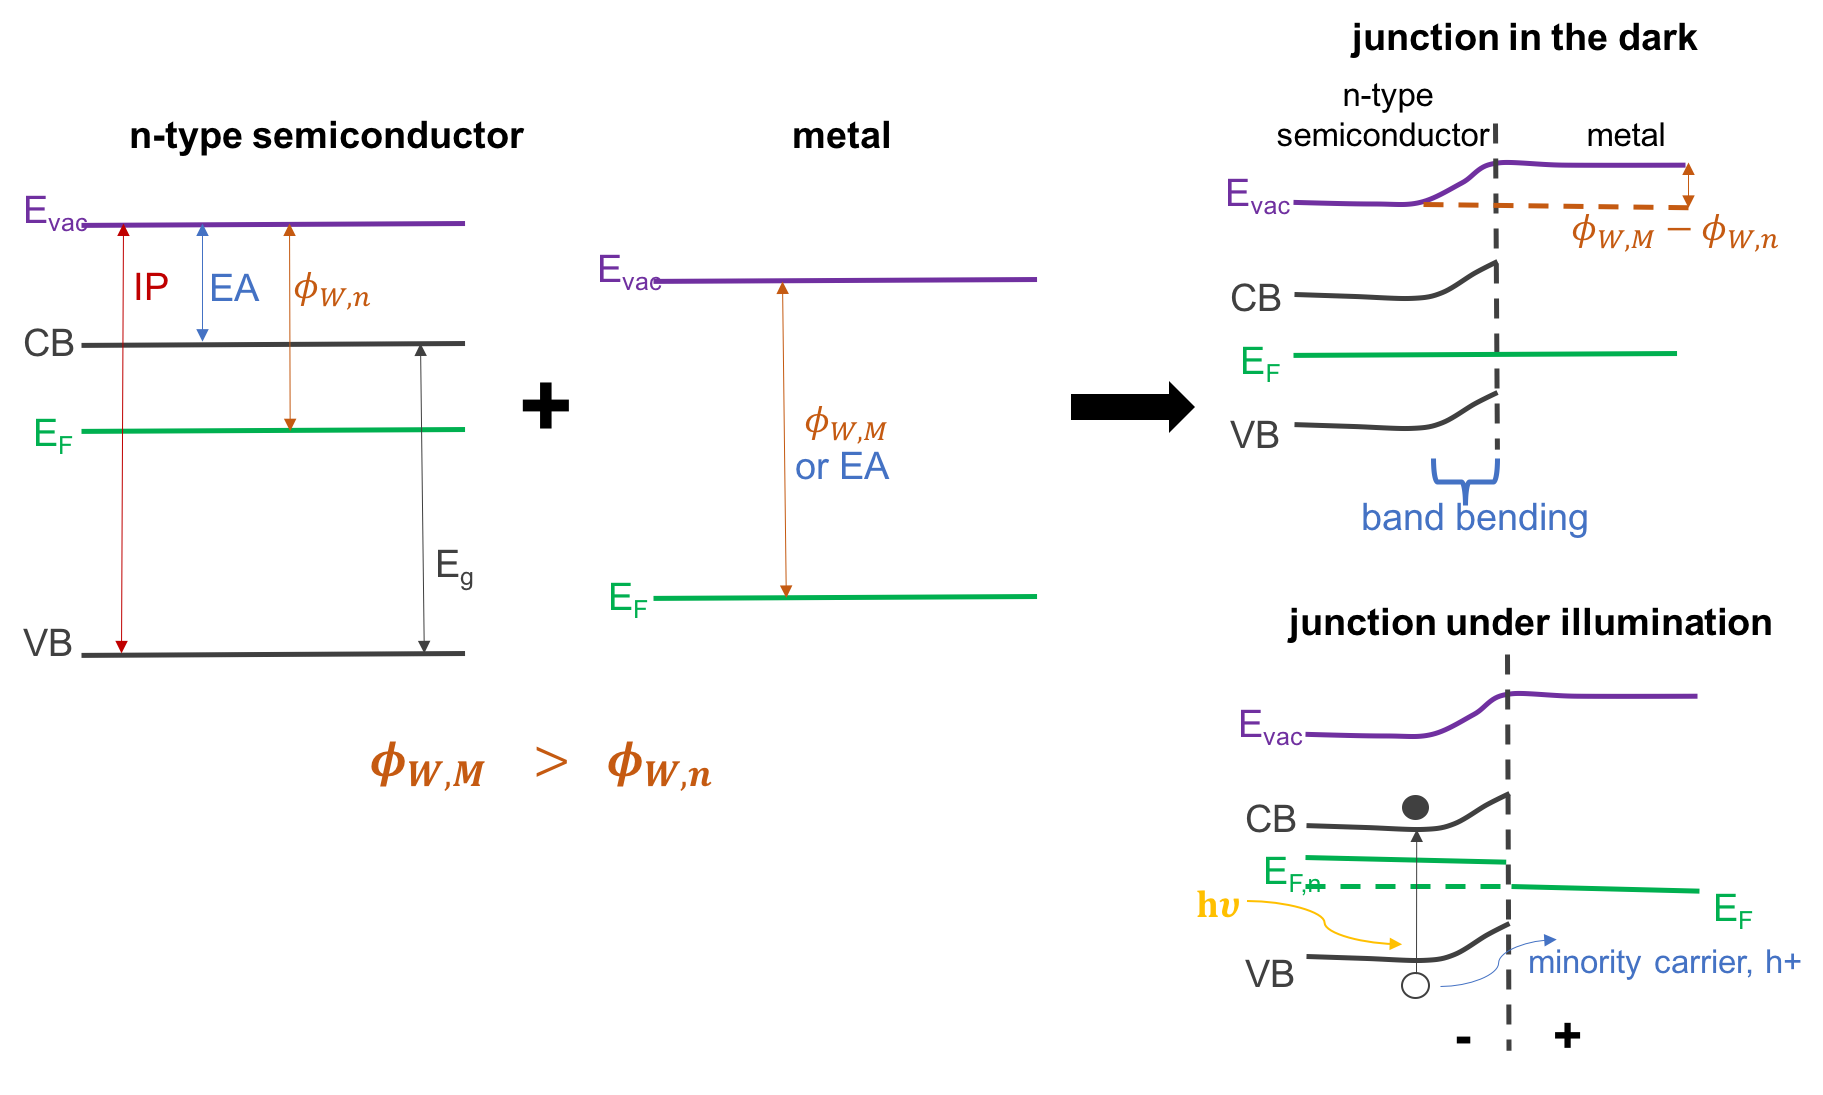
\includegraphics[width=1.0\textwidth]{figures/schottky_schematic.png}
    \caption[The formation of a Schottky barrier junction between an n-type semiconductor and a metal and the splitting of the electron Fermi level ($E_{F,n}$) under illumination]{The formation of a Schottky barrier junction between an n-type semiconductor and a metal and the splitting of the electron Fermi level ($E_{F,n}$) under illumination. Adapted from Ref.~\citenum{Nelson5} and \citenum{band_gap_rev}.}
  \label{schottky_schematic}
\end{figure}

When two materials are isolated, their $E_F$ are independent. When they are brought into electrical contact and allowed to reach thermal equilibrium there is no net current flow. Therefore by definition $E_F$ must be constant across the junction \cite{PV_bands_book}, i.e. the Fermi levels must line up as shown in Fig.~\ref{schottky_schematic}. 
If the two materials have different $\Phi_W$, the vacuum level must then change between the two materials by an amount equal to the difference in $\Phi_W$ between the two materials. The electrostatic field created by a gradient in the vacuum level energy is $\frac{1}{q} \nabla E_{vac}$.
To achieve this gradient, free carriers at the junction redistribute themselves. In the case of a junction between a metal and an n-type semiconductor, if the metal has a larger $\Phi_W$ than the n-type semiconductor, electrons flow from the semiconductor to the metal. A layer of fixed positive charge in the semiconductor and a negative charge on the metal are left behind until a charge gradient builds up that is large enough to prevent any further transport of charge carriers. An electric field that still exists in a material in equilibrium is called a `built-in' electric field \cite{Nelson5}. In this case, the field would drive any excess electrons towards the positively charged side of the junction (the n-type semiconductor) and holes towards the metal side, i.e. it will provide a barrier to the flow of majority n-type carriers from the semiconductor to the metal.

As can be seen in Fig.~\ref{schottky_schematic}, once the semiconductor-metal junction has formed, the CB of the bulk semiconductor is lower than that at the interface, resulting in a spatial variation in electrostatic potential towards the semiconductor-metal interface. This is the region where $E_{vac}$ is changing, the materials possess a net charge and it is called the space-charge or depletion region as it is devoid of any charge carriers \cite{PV_bands_book}. The potential is distributed across the two materials at the interface but drops off further from the interface and the electric field falls to zero.  As metals do not store charge as in a semiconductor, this distance is vanishingly small on the metal side of the junction, but on the semiconductor side this region is typically around 1 micron. The $E_g$ and EA of the semiconductor do not vary, therefore the VB and CB levels change in parallel with $E_{vac}$ at the interface, this effect is called `band bending' and the amount the bands bend is called the `built-in bias', $V_{bi}$.
In the case of a junction between a p-type semiconductor and a metal, if the metal has a smaller $\Phi_W$ than the semiconductor, the semiconductor band instead bends downwards at the interface and presents a barrier to the flow of holes from the semiconductor into the metal, which are now the majority carriers.
If instead $\Phi_W$ of the metal is larger than that of a p-type semiconductor or smaller than that of an n-type semiconductor, the bands will instead bend in such a way as to encourage majority carrier transport across the junction. Majority carriers therefore do not accumulate at the interface to develop the potential difference at the interface necessary for the PVE. This is an Ohmic contact, as opposed to a barrier. 
%Under illumination, photoexcited charge carriers pass easily across the junction and the photovoltage measured at the terminals will be negligible. 

If incident photons have an energy greater than the $E_g$ of the semiconductor in a Schottky barrier junction, then an electron-hole pair can be photoexcited (as depicted in Fig.~\ref{PV_schematic}a). The system is now no longer in equilibrium as the density of electrons and holes has increased and is no longer described by the Fermi-Dirac equilibrium distribution function given in Eq. \ref{fermi-dirac}. 
The space charge region of the junction will cause the photoexcited electron-hole pair to be separated. In the case of a junction between an n-type semiconductor and a metal, electrons will accumulate in the semiconductor and holes in the metal. The semiconductor will become negatively charged and the potential difference across the junction will be reduced. $E_F$ in the semiconductor will now be different for electrons and holes, it has been split into a `quasi-Fermi level' for electrons. Far from the junction the electron quasi $E_F$ will now be larger than in the metal and larger than it was in the semiconductor before illumination, as shown in Fig.~\ref{schottky_schematic}.
There are now different distribution functions for electrons in the CB and holes in the VB. It is assumed that the system reaches a new state of quasi-thermal equilibrium because relaxation of photoexcited electrons within the CB and holes in the VB is on a much faster timescale compared to relaxation between the bands. In each case, the charge carriers are able to establish a new quasi-thermal equilibrium within the bands, with associated quasi-Fermi levels for electrons in the CB and holes in the VB, $E_{F,n}$ and E$_{F,p}$ respectively
\cite{Nelson3}.
 The illumination has generated a photovoltage equal to the difference in the Fermi level in the metal and the semiconductor \cite{Nelson5}. The quasi-Fermi level gradient can be considered as a driving force for conduction \cite{Nelson3}.

A Schottky barrier junction can therefore facilitate photovoltaic energy conversion, but it suffers from certain limitations which impact the maximum achievable photovoltages. For example, a barrier height greater than approximately half of the band gap of the semiconductor will cause minority carriers to outnumber majority carriers close to the interface region, causing an inversion layer. The junction then becomes carrier rich and cannot sustain a photovoltage. Also if the barrier region at the junction is small and the semiconductor layer is highly doped, tunneling of majority carriers across the junction may occur, reducing the effectiveness of the barrier. Many of these problems can be overcome by using a semiconductor-semiconductor p-n junction \cite{Nelson5}, outlined next.

\subsection{Semiconductor p-n junctions}
\begin{figure}[h!]
  \centering
    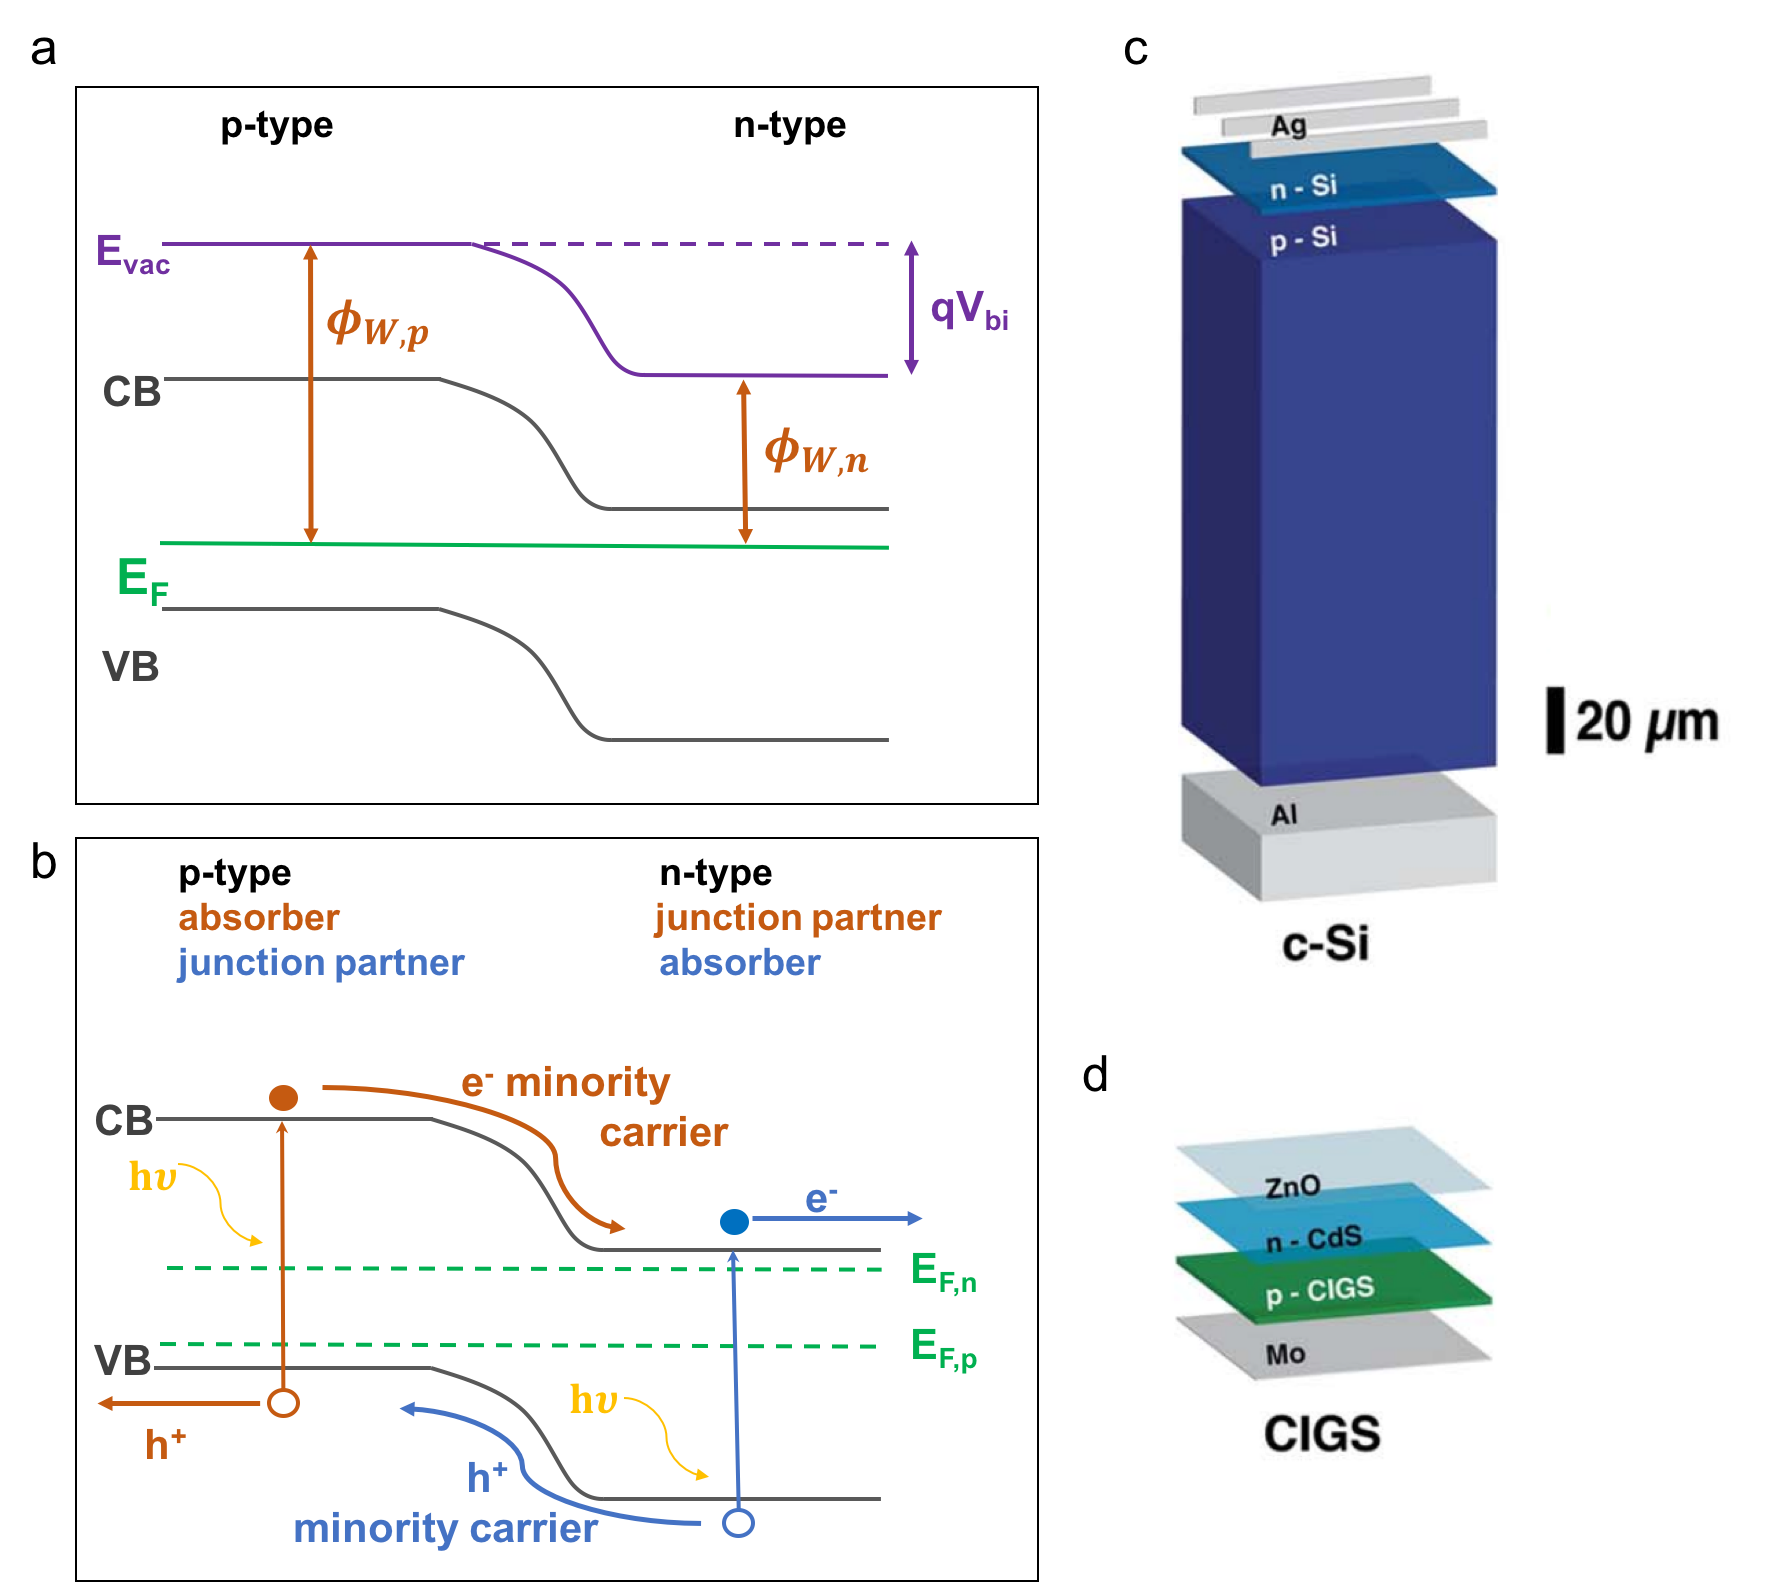
\includegraphics[width=0.85\textwidth]{figures/p-n_schematic.png}
    \caption[p-n junction formed between a p-type and n-type semiconductor, in the dark and in thermal equilibrium indicating the difference in work functions ($\Phi_W$) and built-in bias ($V_{bi}$) (a). p-n junction under illumination indicating the direction of flow of minority carriers in the case of a p-type (orange) and n-type (blue) absorber layer (b). Schematic of device architecture for a silicon wafer-based device (c) and a CIGS thin-film device architecture (d).]{p-n junction formed between a p-type and n-type semiconductor, in the dark and in thermal equilibrium indicating the difference in work functions ($\Phi_W$) and built-in bias ($V_{bi}$) (a). Adapted from Ref.~\citenum{Nelson5}. p-n junction under illumination indicating the direction of flow of minority carriers in the case of a p-type (orange) and n-type (blue) absorber layer (b). Adapted from Ref.~\citenum{Nelson6}. Schematic of device architecture for a silicon wafer-based device (c) and a CIGS thin-film device architecture (d), both figures reproduced with permission from Ref.~\citenum{pathways}.}
  \label{p-n_schematic}
\end{figure}

For certain semiconductors, such as Si, it is possible for the material to be doped both n- and p-type depending on the valence of the dopant species relative to the host lattice, i.e. it is ambipolar. In this case, it is possible to form a junction between electrically distinct p-type and n-type semiconductors by doping different regions of the same material differently to form a `homojunction'. An example PV architecture for a Si solar cell is shown in Fig.~\ref{p-n_schematic}c. Since $\Phi_W$ of the p-type is larger than that of the n-type region, an electric field is established at the junction due to the difference in electrostatic potential, as shown in Fig.~\ref{p-n_schematic}a. Under illumination this will drive photoexcited electrons towards the n-type layer and holes towards the p-type layer, as shown in Fig.~\ref{p-n_schematic}b. The junction region is depleted of both electrons and holes \cite{Nelson5}.

%In real, non-ideal, solar cell devices power is dissipated through parasitic resistances in the device, including current leakage and resistance from the electrical contacts \cite{Nelson1}. In the case of the p-n junction architecture shown schematically in Fig \ref{PV_architecture}b, there can be series resistance of the p and n layers to the flow of majority carriers, resulting in a reduction in the potential between the junction and the terminal. There can also be resistance at the contact layers in the device, such as those indicated in Fig. \ref{PV_architecture}c and \ref{PV_architecture}d \cite{Nelson6}. The open circuit voltage (V$_{OC}$) of a device can be reduced by non-ideal alignment of the electronic bands of the different layers within the device. 
For many of the materials being studied for use as absorber layers in thin-film solar cells, such as chalcogenide-based materials like the device shown in Fig.~\ref{p-n_schematic}d, it is not possible, or is very difficult, to achieve ambipolar doping \cite{band_alignment_review, Zhang_doping_limits}. Therefore to achieve a p-n junction for many thin-film PV devices it is necessary to form an interface between two different materials with different energy gaps, lattice constants and even slightly different crystal structures. Due to such mismatches, defects are expected to be more prevalent at heterojunction interfaces than at homojunction interfaces. In section \ref{sulfosalt_band_alignment} band alignments that have been proposed for reducing the impact of defects at p-n heterojunctions will be discussed and suggestions for heterojunction partners for the candidate photoferroic solar absorber materials are presented.


\section{Absorber material properties for efficient solar cells}\label{PV_properties}
The most fundamental, necessary requirement for a solar absorber material in a PV device is that it possesses a band gap (E$_g$) across which an electron can be excited. As discussed in the previous section, the magnitude of this E$_g$ must also be somewhere within the energy range of the solar spectrum so that sunlight can induce this excitation. The next most fundamental requirement of a solar absorber material is that it must allow for the transport of charge carriers out of the absorber material layer, into a collection electrode and on to an external circuit in order to do electrical work. Provided these necessary conditions are met and some sort of spatial asymmetry (outlined above) is present to drive electrons away from their point of promotion, the material should exhibit the PVE \cite{Nelson2}. However, how well it will actually peform in a solar cell is determined by more stringent criteria and other material properties. 

\subsection{Electronic band gap and optical absorption}

Firstly, the actual value of the E$_g$ within the range of the solar spectrum (shown in Fig.~\ref{PV_schematic}b) is of importance. It is ideal for the value to be as close as possible to the region of photon energies that make up the majority of the solar spectrum. The optimal range for E$_g$ under typical radiation conditions is approximately 1.0 to 1.7 eV \cite{PV_E_range}. The upper limit of the power conversion efficiency (PCE) of incident photon energy into electrical energy by a device made from a particular absorber material based on its E$_g$ was first calculated by Shockley and Quiesser in 1961 \cite{SQ_1961}. A plot of theoretical efficiency limit as a function of E$_g$ was shown in Fig.~\ref{SQ}, as well as the record efficiencies of various PV technologies.

\begin{figure}[h!]
  \centering
    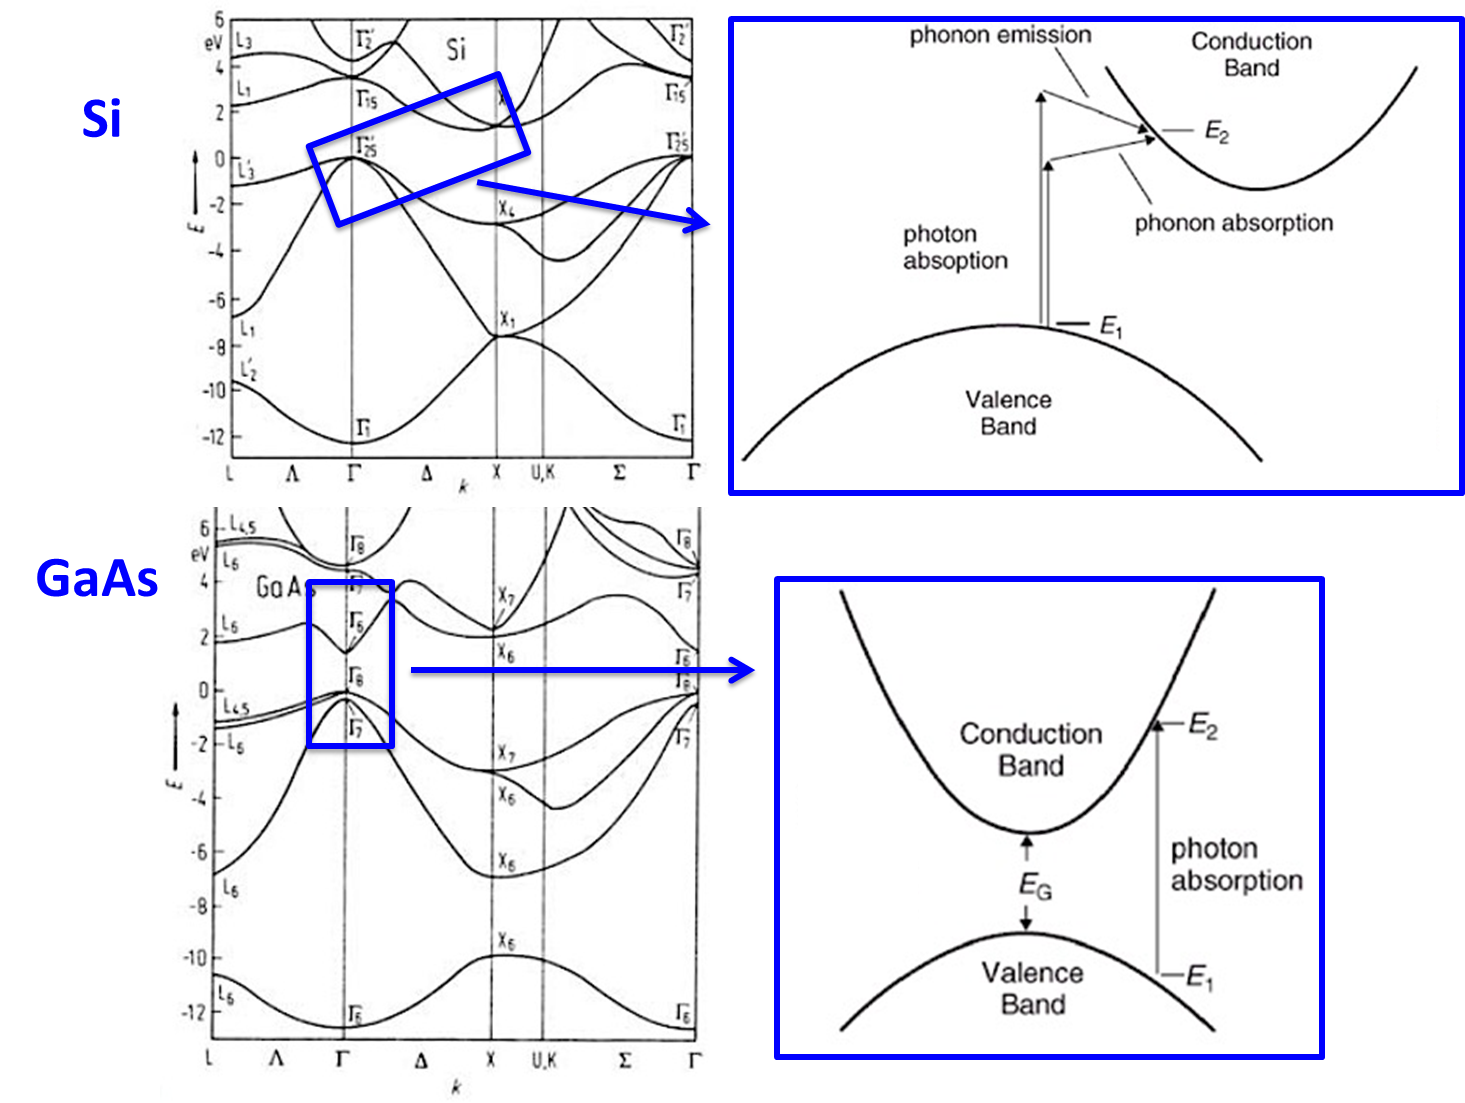
\includegraphics[width=0.95\textwidth]{figures/Si_and_GaAs.png}
    \caption[The electronic band structure of silicon and a schematic of the absorption process in an indirect band gap semiconductor (top). The band structure of GaAs and schematic of the absorption process in a direct gap semiconductor.]{The electronic band structure of silicon and a schematic of the absorption process in an indirect band gap semiconductor (top). The band structure of GaAs and schematic of the absorption process in a direct gap semiconductor. Fig. adapted from Ref.~\citenum{phys_semicond} and \citenum{PV_bands_book}.}
  \label{Si_and_GaAs}
\end{figure}

However, it is not only the value of E$_g$ that is of importance. More intricate details of the band structure of the material can also impact on the performance of a solar cell device made from the material. Whether the band structure shows a band gap that is direct or indirect can have an impact on the performance of a solar cell made from the material. Fig.~\ref{Si_and_GaAs} shows the band structures of Si and GaAs, where Si possesses an indirect band gap and GaAs possesses a direct band gap, i.e. the extrema of the VB and CB occur at the same value of \textbf{k} for the latter but not for the former. The excitation of an electron from the valence band maximum to the conduction band minimum is called fundamental absorption, as there are several other optical absorption transitions that can occur in a semiconducting material, especially in a defective material, and this point will be discussed more in section \ref{defects_impact}. Both the total energy and momentum of all particles involved in the absorption process must be conserved. Photons do possess momentum ($\frac{h}{\lambda}$), however, this is very small compared to the range of crystal momenta and so the electron momentum is effectively conserved during photon absorption. For a direct transition, the absorption coefficient of a material for a given photon energy, $h \nu$, is proportional to the probability, p$_{12}$, of the transition of an electron from the initial state E$_1$ to the final state E$_2$, the density of electrons in the initial state, $g_{v}(E_1)$, and the density of available final states, $g_{c}(E_2)$. This is then summed over all possible transitions between states where $E_2 - E_1 = h\nu$. Since the electron momentum is conserved during a direct transition, the crystal momentum in the valence band is approximately the same as that of the final state in the conduction band at energy $E_2$ \cite{PV_bands_book}.

However, for an indirect band gap semiconductor, such as silicon shown at the top of Fig.~\ref{Si_and_GaAs}, the valence band maximum occurs at a different crystal momentum to that of the conduction band minimum. As discussed earlier, the momentum of a photon is far less than that of crystal momenta. In order to conserve the momentum of an electron during an optical transition across an indirect band gap, momentum must be either provided by the lattice or released to the lattice usually in the form of the particle representation of a lattice vibration, known as a phonon, as indicated in the top right schematic of Fig.~\ref{Si_and_GaAs}. Since both a phonon and an electron are needed to make an indirect transition possible, the optical absorption coefficient, $\alpha$, depends not only on the density of states of the electrons, as for a direct transition, but also on the availability of emitted or absorbed phonons with the required momentum. Therefore, $\alpha$ for an indirect transition compared to a direct transition is typically relatively small and more heavily dependent on temperature \cite{Nelson3}. 

\begin{figure}[h!]
  \centering
    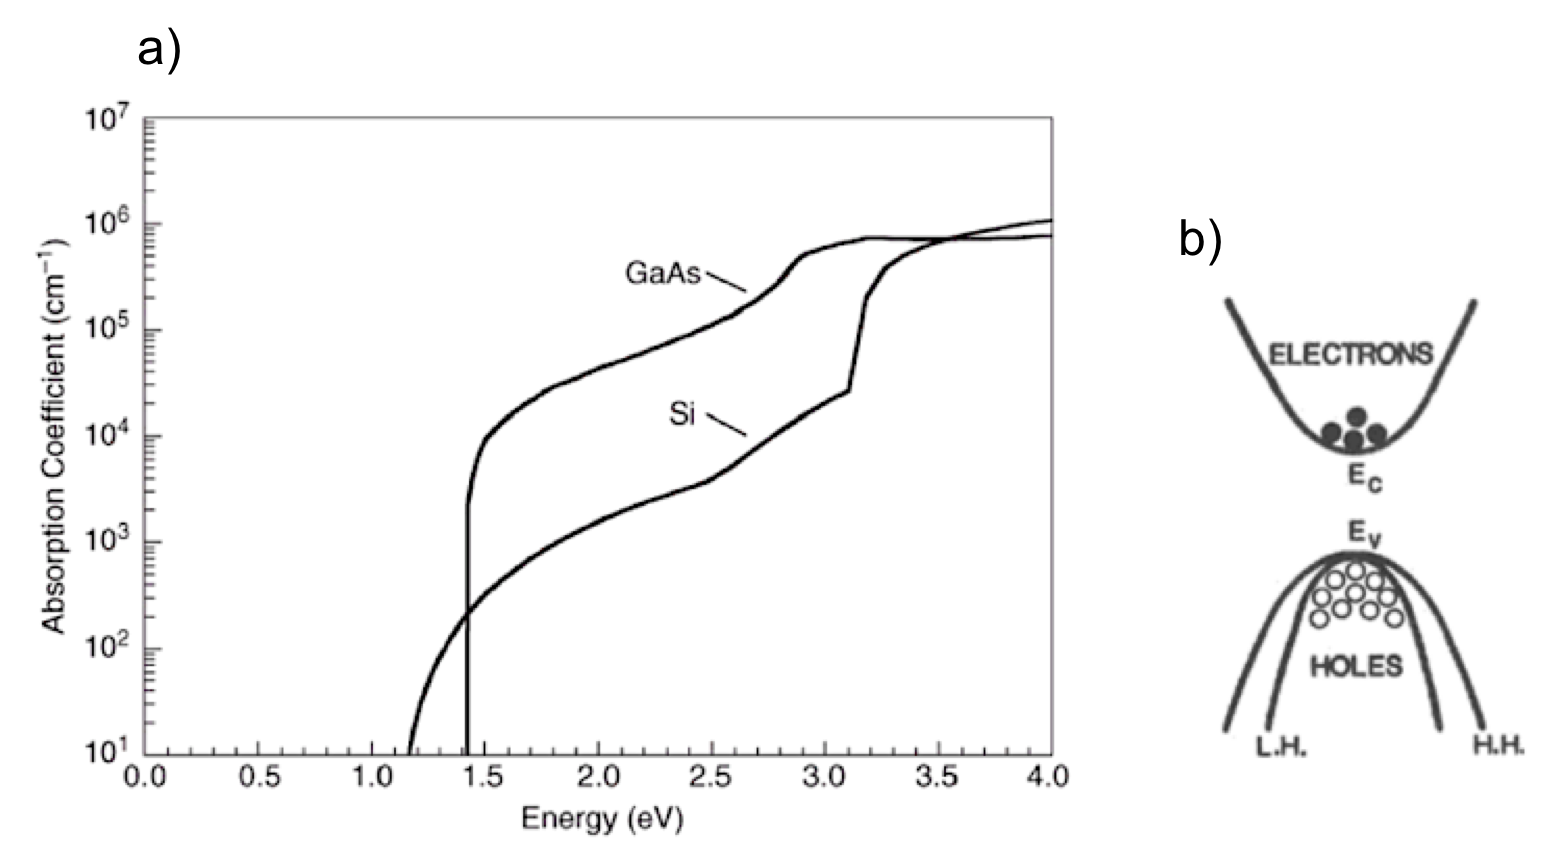
\includegraphics[width=0.95\textwidth]{figures/ab+m_eff.png}
    \caption[a) A comparison of the absorption coefficients of the indirect band gap semiconductor Si and the direct band gap semiconductor GaAs across a range of incident photon energies. b) Schematic of a the band structure of a photoexcited semiconductor with electrons near the bottom of the conduction band, holes near the top of the valence band, where the particular material has both heavy- and light-hole bands (labelled H.H and L.H in the figure respectively).]{a) A comparison of the absorption coefficients of the indirect band gap semiconductor Si and the direct band gap semiconductor GaAs across a range of incident photon energies. Figure reproduced with permission from Ref.~\citenum{PV_bands_book}. b) Schematic of a the band structure of a photoexcited semiconductor with electrons near the bottom of the conduction band, holes near the top of the valence band, where the particular material has both heavy- and light-hole bands (labelled H.H and L.H in the figure respectively). Figure reproduced with permission from Ref.~\citenum{heavy_holes}.}
  \label{ab+m_eff}
\end{figure}

The $\alpha$ of a material determines the penetration depth, $\frac{1}{\alpha}$, of light incident on the material \cite{absorption_coeff_book1}. Fig.~\ref{ab+m_eff}a shows the absorption coefficients of GaAs and Si across a range of wavelengths. The figure shows a less steep onset of absorption for Si compared to GaAs As discussed earlier, Si possesses an indirect band gap, while GaAs possesses a direct band gap. 
The implication of the differing $\alpha$ and therefore different optical penetration depths of absorber layers is that materials which are stronger absorbers require less material to absorb the light. This forms the basis of thin-film solar cell technologies.
On the other hand, materials with a weaker onset of absorption, as is often the case for materials with an indirect band gap such as Si, a thicker layer of absorber material is required to absorb the same amount of light \cite{PV_bands_book}. This is undesirable if the particular material contains rare or expensive components and also results in higher demands on material quality as charge carriers must be transported through the absorber material in order to be collected.
Thin-film PV technologies typically require a less high-quality and defect-free absorber layer as charge carriers do not have to travel through as much of the material in order to reach a collection electrode. However, defects in the absorber layer do still play a decisive role in determining the device performance of thin-film film PV technology, and this point is discussed much more in section \ref{defects_impact}.

\subsection{Charge-carrier effective mass}

As mentioned in section \ref{BandTheorySection}, another property of importance that can be derived from the electronic band structure of a material, i.e. the plot of E(\textbf{k}) vs. k, is the effective mass, m*. m* is related to the curvature of the band at the top of the VB (for holes) or at the bottom of the CB (for electrons). m* can be calculated by a quadratic least-squares fit to the band extrema when using the parabolic approximation. The curvature of the plot can then be used to obtain m* with Eq. \ref{m*_fit}.
\begin{equation}\label{m*_fit}
m^* = \left( \frac{1}{\hbar^2}\frac{\partial^2 E}{\partial k^2} \right)^{-1}
\end{equation}
However, just from a quick inspection of the band structure of a material, a more steeply curved shape to the band extrema indicates a lower effective mass and therefore satisfies a necessary condition for higher carrier mobility. Fig.~\ref{ab+m_eff}b shows a schematic of the band structure of a direct band gap semiconductor that has both heavy- and light-hole bands at the valence band maximum, where the flatter band corresponds to the heavy-hole band.
The m* of electrons or holes are the masses they seem to carry for transport properties \cite{dielectric_const1}. For example, in ZnSnO$_3$ the hole m* has been calculated to be large, indicating that hole mobility will be poor in this material. Poor mobility will make carrier extraction difficult, which has been linked to the low photocurrents observed in this material \cite{effective_mass1}.
%Although certain thin-film technologies, which will be discussed towards the end of section \ref{current_tech}, reduce the amount of absorber material the charge carrier must travel through before being collected. So although carriers must still travel through the material, effective mass could be considered less of a crucial parameter for this technology. 
However, a small m* should just be considered as a necessary but not a sufficient condition for good carrier mobility as the effect of the effective mass on the transport properties could be overshadowed by other factors, such as the scattering of charge carriers by defects in a real, non-ideal material. 

\section{Impact of absorber layer defects on solar cell performance}\label{defects_impact}
%Refer to: pg 160 \cite{fund_semi}, pg 51, 52, 64 \cite{thin_film_Boer}, pg 63 + 65 \cite{phys_semicond}\\
Although the main framework for modelling solid-state systems (as outlined at the start of this chapter) is built around perfect, periodic systems; in reality absolutely perfect systems do not exist. Deviations from the perfect crystal lattice structure (i.e. defects) can strongly influence the performance of electronic devices. There is an energy cost associated with the creation of a defect, but in many cases the free energy of a system can be lowered by the incorporation of a certain concentration of defects due to an increase in the configurational entropy of the system \cite{AshcroftMermin_general}. Methods for modelling defects in solids are discussed in section \ref{defects_methods}, but here the impact of defects in the absorber layer on the performance of a solar cell is discussed.

\subsection{Types of crystal defect}

There are many different possible types of crystal defect. If a defect does not involve any atoms that are foreign to the host crystal, then the defect is called an intrinsic or native defect. Defects involving foreign atoms (impurities) are referred to as extrinsic defects. Fig.~\ref{defects}b and \ref{defects}c show some examples of extrinsic and intrinsic defects. This work is primarily interested in the fundamental material properties of candidate solar absorber materials, so only intrinsic defects are considered. In real systems, however, impurities are sometimes unintentionally present in the growth or processing environment, or may be introduced intentionally to tune the optoelectronic properties of the material.
Defects are usually classified as point or extended defects. Point defects usually involve isolated atoms in localised regions of a host crystal, such as those shown in Fig.~\ref{defects}b and \ref{defects}c. There are a number of different possible point defects, such as: vacancies, interstitials and antisites, which correspond to the removal, insertion or substitution of species from the perfect host lattice respectively. Extended defects may involve rows of atoms, such as a dislocation defect. An example of a line defect is shown in Fig.~\ref{defects}a. Another possible type of defect is a defect complex, which is composed of a small number of point defects.

\begin{figure}[h!]
  \centering
    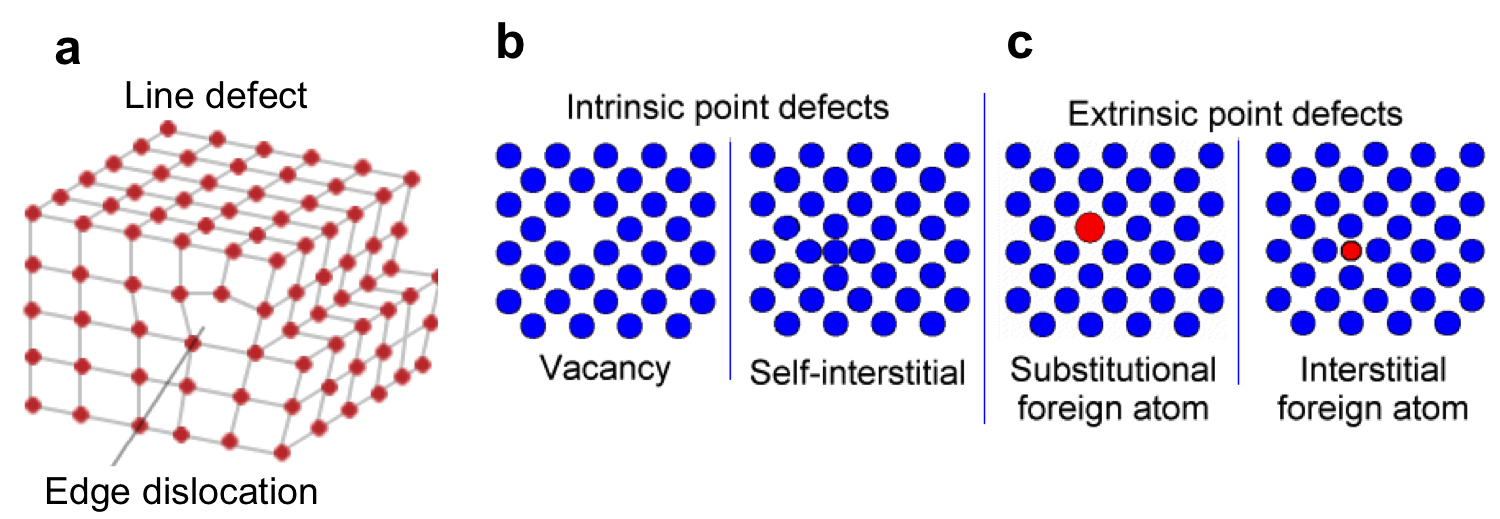
\includegraphics[width=0.9\textwidth]{figures/defects.png}
    \caption[An example of a line defect (a) and both intrinsic (b) and extrinsic (c) point defects.]{An example of a line defect (a) and both intrinsic (b) and extrinsic (c) point defects. Figure reproduced with permission from Ref.~\citenum{defects_fig1} and \citenum{defects_fig2} respectively.}
  \label{defects}
\end{figure}

The electrical properties of semiconductors can be modified significantly by the incorporation of very small amounts of impurities or defects. It is often the case that less than one defect per million of host atoms is sufficient to alter the properties of a semiconductor \cite{fund_semi}. This sensitivity to defects is one of the reasons why semiconductors find many uses in device applications. For example, luminescence centres in wide-band-gap materials can be used to emit light at specific wavelengths or single-spin centres provided by defects can act as artificial atoms and serve as a qubit in a quantum computer \cite{defects_tutorial}. In order to control the electrical properties of a material by introducing defects, typically processes must first be developed to produce a fairly defect-free material, before intentionally introducing particular defects \cite{fund_semi}. In the case of solar cell devices, however, the presence of defects can be detrimental depending on the nature of the defect \cite{Aron_defect_tolerance}, which will be discussed next. 

\subsection{Optical properties of defective solids}\label{defect_theory}
\subsubsection{Low defect concentrations}

When defects are present at sufficiently low concentrations such that defect-defect interactions are neglible, the defects are considered isolated point defects in the `dilute limit'. Certain point defects result in additional energy levels in between the valance-band maximum (VBM) and conduction-band minimum (CBM), i.e. within the band gap of the material. An example for intrinsic point defects in the absorber material {\CZTS} is shown in Fig.~\ref{defects_CZTS}. Electrically active defects have at least one charge state for the defect that produces a defect level in the band gap. This level then has an associated defect wavefunction, a state to which the electron is added to or removed when the charge state of the defect changes. If the defect level is positioned close enough to the band edges such that the defect is likely to be thermally ionised at room temperature, then the defect is conventionally referred to as `shallow'. If the defect produces a level in the band gap and far from the band-edge, it is a referred to as `deep'.  Another way of defining a defect as `shallow' or `deep' is based on the degree of localisation of the wavefunction. If a defect wavefunction is delocalised (on the order of many lattice constants) then the defect has the characteristics of a shallow defect. If the wavefunction is instead localised on the length scale of an atomic bond then this indicates a deep level defect \cite{defects_tutorial}. 

\begin{figure}[h!]
  \centering
    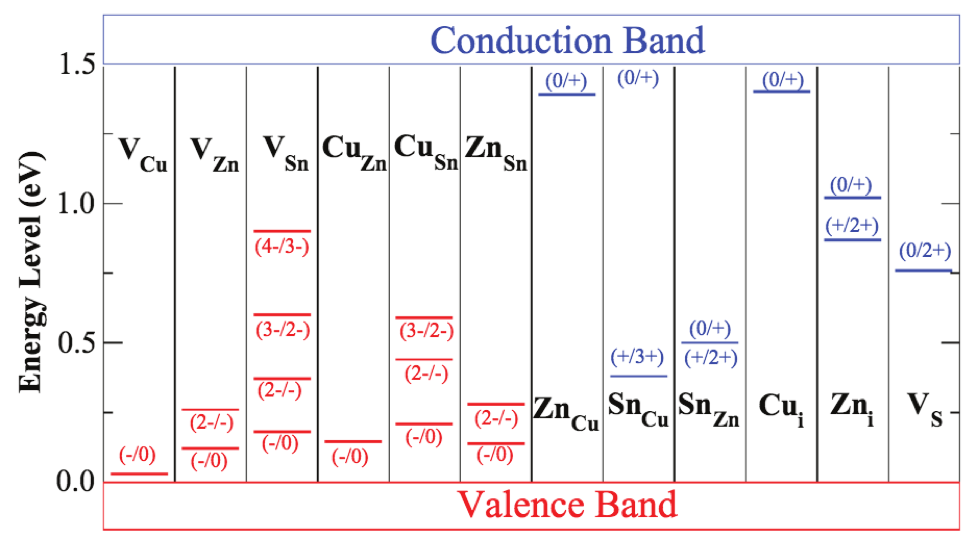
\includegraphics[width=0.7\textwidth]{figures/Chen_CZTS_defects.png}
    \caption[Ionisation levels of intrinsic point defects in the band gaps of {\CZTS}]{Ionisation levels of intrinsic point defects in the band gaps of {\CZTS}. Figure reproduced with permission from Ref.~\citenum{defects_Chen_large}.}
  \label{defects_CZTS}
\end{figure}

There are different `flavours' of defects \cite{Aron_defect_tolerance}. Shallow defects can be beneficial to improve electrical conductivity for carrier extraction from an absorber materials. Typically deep levels are thought to be the most detrimental to solar cell device performance \cite{Stoneham_killer_defects}. 
Defects that produce mid-gap states act as Shockley-Read-Hall recombination sites \cite{SRH}, which is regarded as the most important recombination process in real, non-perfect semiconductors. It is a form of non-radiative recombination where a charge carrier is trapped in the defect state before recombining with a charge carrier of opposite polarity. This type of recombination is known to be detrimental to device performance as it essentially results in energy input from sunlight not being converted into electricity \cite{Nelson4}.

\begin{figure}[h!]
  \centering
    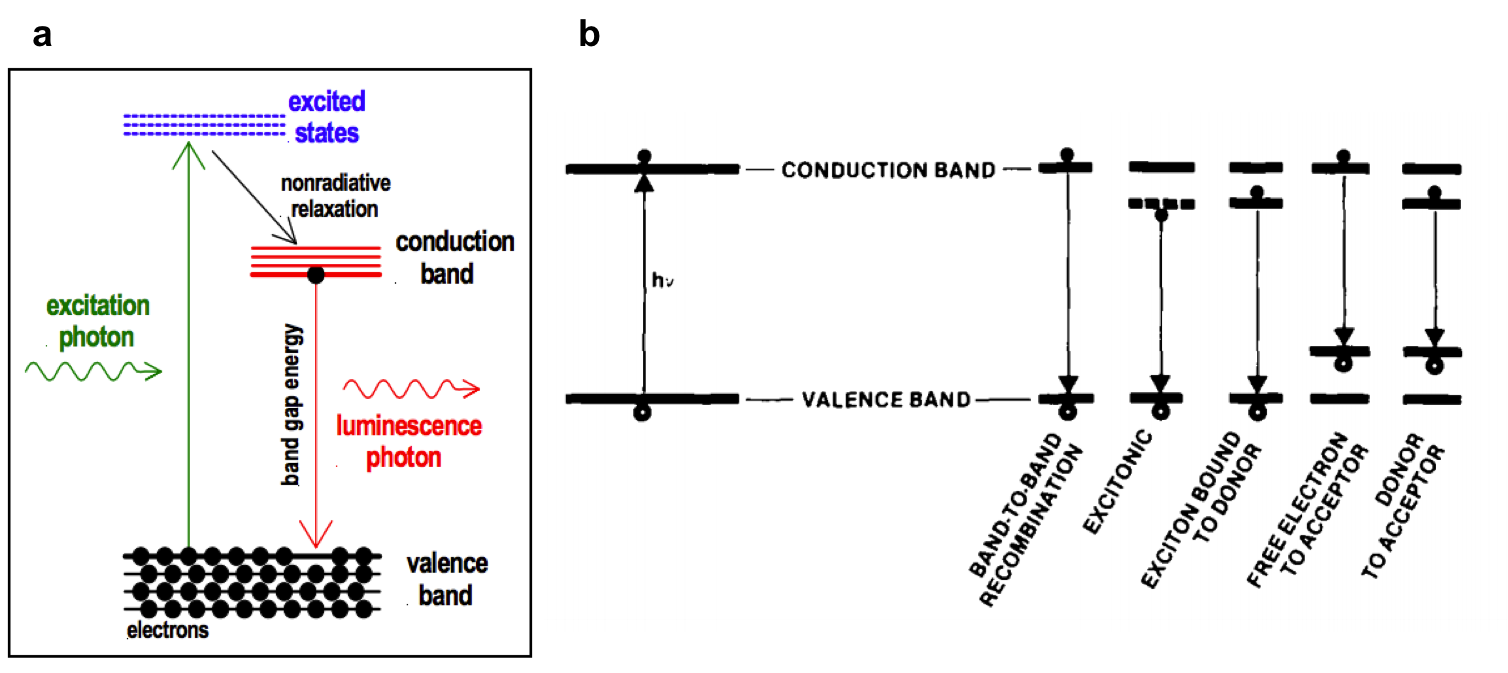
\includegraphics[width=1.0\textwidth]{figures/PL_transitions.png}
    \caption[Basic optical transitions involved in a measurement during photoluminescence spectroscopy (a). Common emission transitions detected during photoluminescence measurements, including transitions involving defect levels (b).]{Basic optical transitions involved in a measurement during photoluminescence spectroscopy (a). Common emission transitions detected during photoluminescence measurements, including transitions involving defect levels (b). Figure reproduced with permission from Ref.~\citenum{PL_transitions} and \citenum{Pankove} respectively.}
  \label{PL_transitions}
\end{figure}

Photoluminescence (PL) measurements are able to pick up optical signatures of defects even if they are present at low concentrations with high resolution. 
In a PL experiment, photons with energies larger than that of the band gap excite electrons from the valence band to the conduction band, as shown in Fig.~\ref{PL_transitions}a. In addition, electrons can be excited from or relax to defect levels, as shown in Fig.~\ref{PL_transitions}b. When the excited electrons transition to lower energy levels, they can emit light to conserve energy, resulting in a peak in the PL spectrum. In a PL excitation experiment, the PL intensity is measured as a function of excitation photon energy. This gives an absorption profile for the defects.
PL measurements alone however cannot be used to identify the character of a defect, this is an area where first-principles defect calculations can provide some insight \cite{defects_tutorial}.


\subsubsection{High defect concentrations}
The energy band model described in section \ref{BandTheorySection} has been successful in explaining many aspects of the behaviour of solids and a large amount of experimental data has supported the theoretical predictions made using this model. Its main drawback is that it assumes a perfect, or nearly perfect, crystal lattice. It applies well to single crystals and polycrystalline substances, but omits important physical characteristics when used to study materials that are amorphous or heavily disordered such that the structure deviates significantly from the periodicity of the crystal \cite{small_semiconductor1}.
Low concentrations of impurities and defects can be modeled by considering the introduction of distinct additional donor and acceptor energy levels within the band gap of a material (as discussed above) and the scattering of electrons and holes in the solid. 
%\begin{figure}[h!]
%  \centering
%    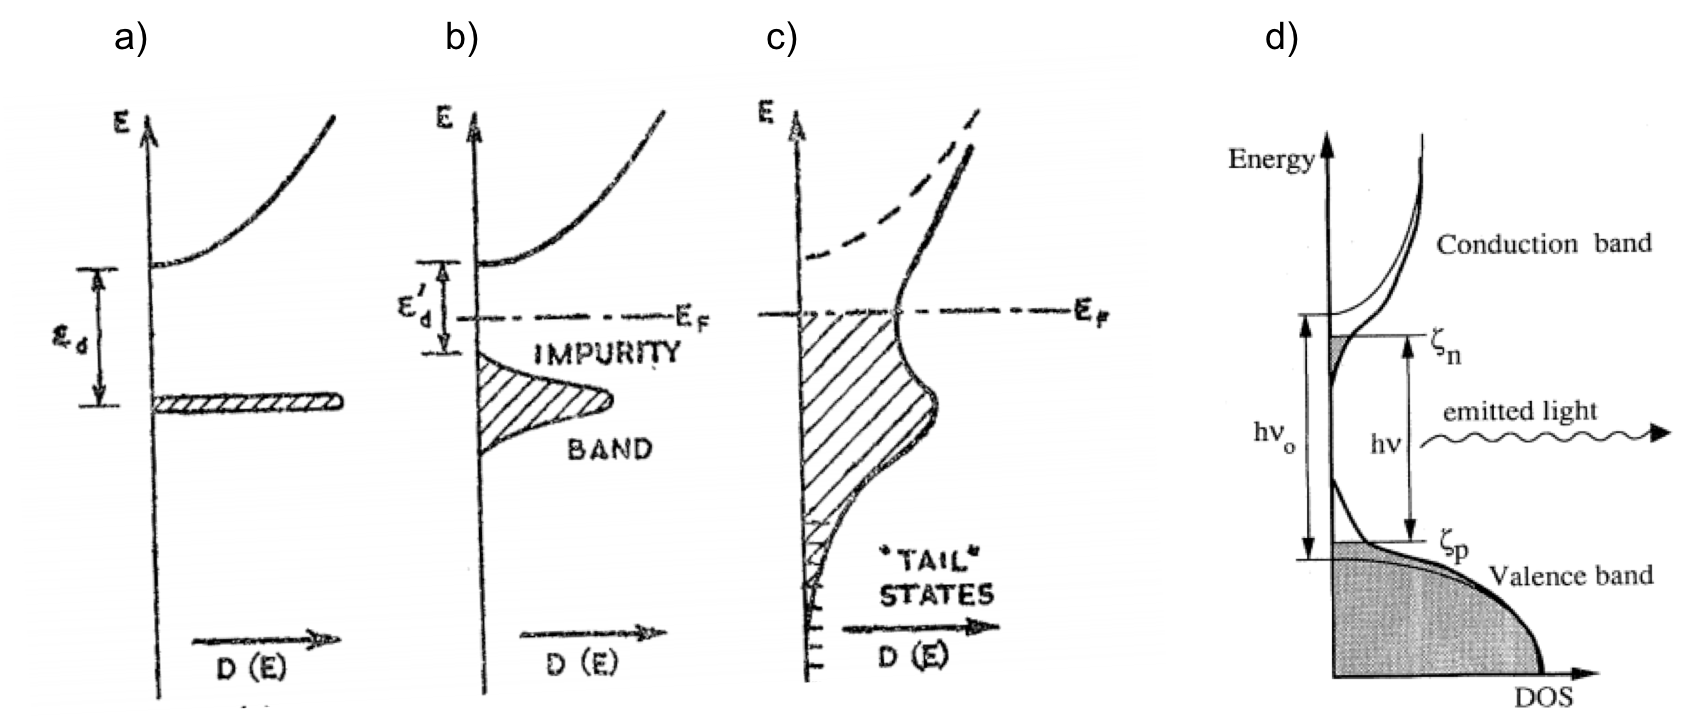
\includegraphics[width=1.0\textwidth]{figures/bs2+pankove.png}
%    \caption[The influence of increased donor impurity density on the conduction band profile showing low (a), medium (b) and high (c) densities of impurities. (d) Schematic of band tailing. $\zeta_{n,p}$ are the quasi-Fermi level for electrons and holes respectively. The narrow line denotes the unperturbed density of states (DOS), while the heavy line depicts the DOS modified by heavy-doping effects. Both valence and conduction bands are shifted towards each other to give a narrowing of the band gap and the DOS is distorted, showing band tails.]{The influence of increased donor impurity density on the conduction band profile showing low (a), medium (b) and high (c) densities of impurities. Figure reproduced with permission from Ref.~\citenum{small_semiconductor2}. (d) Schematic of band tailing. $\zeta_{n,p}$ are the quasi-Fermi level for electrons and holes respectively. The narrow line denotes the unperturbed density of states (DOS), while the heavy line depicts the DOS modified by heavy-doping effects. Both valence and conduction bands are shifted towards each other to give a narrowing of the band gap and the DOS is distorted, showing band tails. Figure reproduced with permission from Ref.~\citenum{Pankove}.}
%  \label{bs2}
%\end{figure}

\begin{figure}[h!]
  \centering
    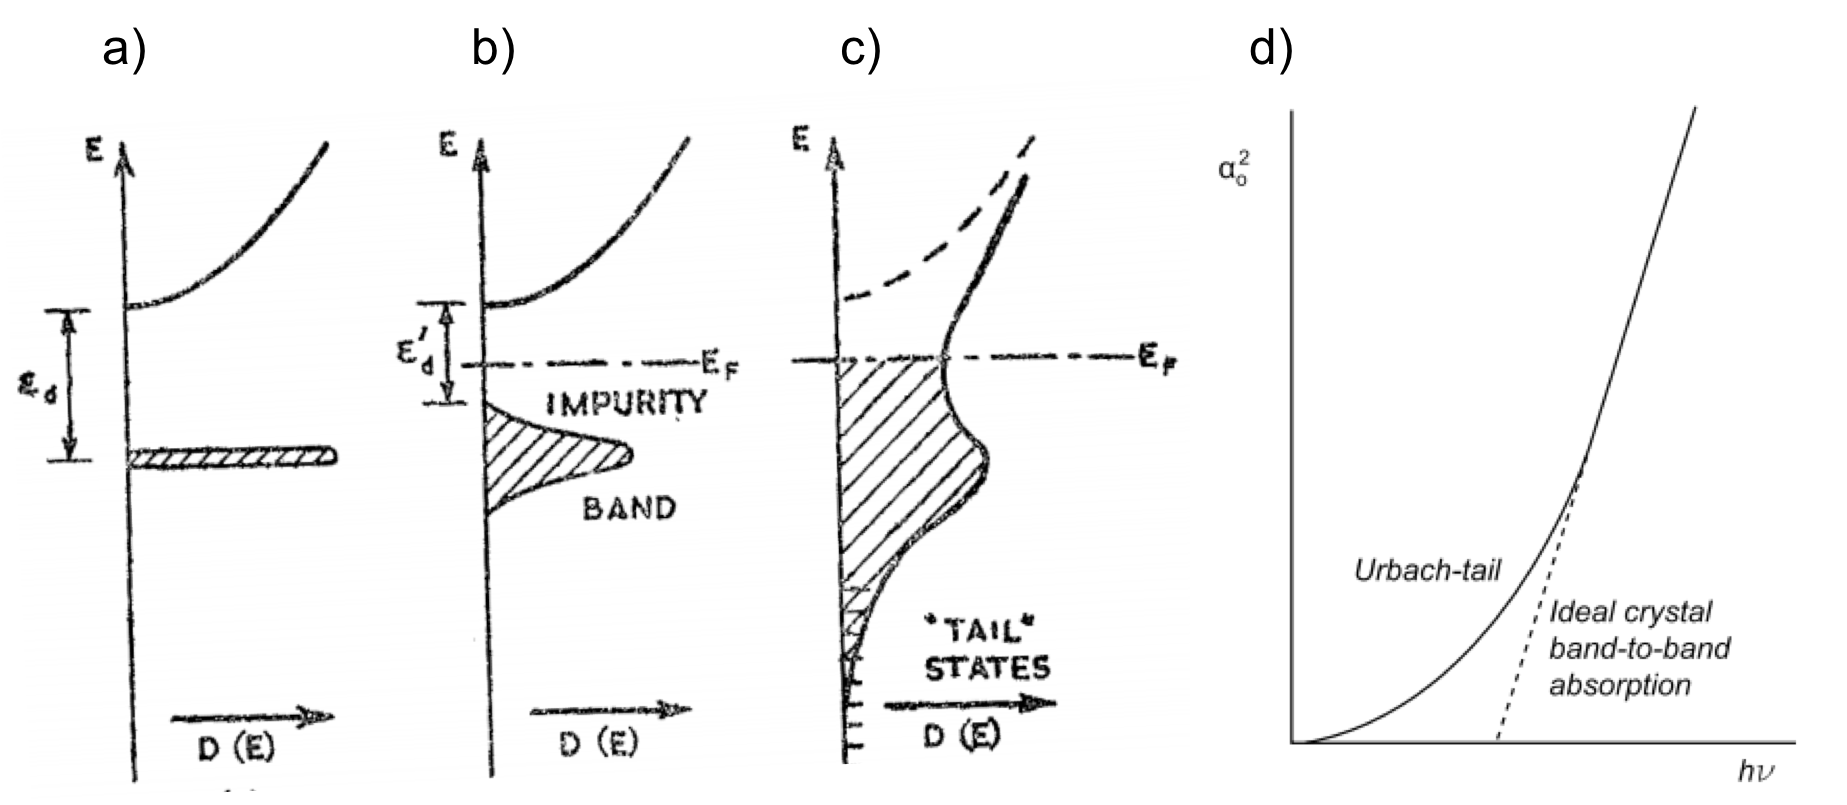
\includegraphics[width=1.0\textwidth]{figures/bt+u.png}
    \caption[The influence of increased donor impurity density on the conduction band profile showing low (a), medium (b) and high (c) densities of impurities. (d) Optical absorption spectrum of a typical direct band gap semiconductor with the absorption coefficient, $\alpha_{0}$, proportional to the extended density of states in the Urbach tail.]{The influence of increased donor impurity density on the conduction band profile showing low (a), medium (b) and high (c) densities of impurities. Figure reproduced with permission from Ref.~\citenum{small_semiconductor2}. (d) Optical absorption spectrum of a typical direct band gap semiconductor with the absorption coefficient, $\alpha_{0}$, proportional to the extended density of states in the Urbach tail. Figure reproduced with permission from Ref.~\citenum{thin_film_Boer}.}
  \label{bs2}
\end{figure}

At higher defect concentrations, it is possible to observe a phenomena called `band tailing'. At sufficiently high concentrations, defect levels interact to form a band. For example, for high n-type doping the impurity band merges with the conduction band, causing a rigid shift of the conduction band towards the valence band \cite{Pankove}. The band profile can be modified with increasing donor density as shown in Fig.~\ref{bs2}a-c. 
%to give rise to conductivity even at temperatures that are too low to produce excitation of carriers into the free conduction bands, called impurity band conduction \cite{small_semiconductor2}.
%In heavily-doped semiconductors it is possible to observe a phenomena called `band tailing', where the valence and conduction bands are shifted towards each other resulting in a narrowing of the band gap, as shown in Fig.~\ref{bs2}d \cite{Pankove}. 
%The heavy-doping effects then result in a different emitted spectrum which can be detected by techniques such as photoluminescence (PL) spectroscopy. 

Such a tail of band states into the band gap is often referred to as a Lifshitz tail \cite{Lifshitz1964}, it can be observed experimentally and is most noticeable in heavily doped and amorphous semiconductors \cite{thin_film_Boer}. 
%\begin{figure}[h!]
%  \centering
%    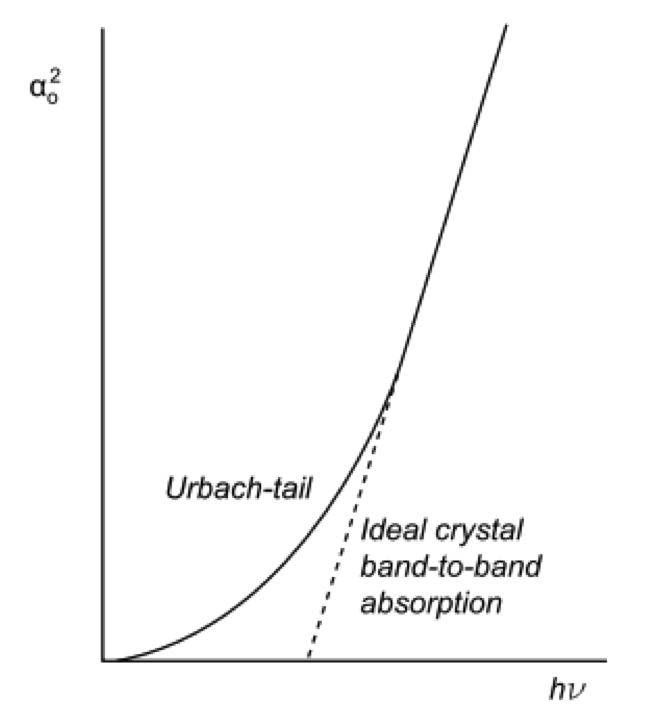
\includegraphics[width=0.45\textwidth]{figures/urbach_fig.png}
%    \caption[Optical absorption spectrum of a typical direct band gap semiconductor with the absorption coefficient, $\alpha_{0}$, proportional to the extended density of states in the Urbach tail.]{Optical absorption spectrum of a typical direct band gap semiconductor with the absorption coefficient, $\alpha_{0}$, proportional to the extended density of states in the Urbach tail. Figure reproduced with permission from Ref.~\citenum{thin_film_Boer}.}
%  \label{urbach_fig}
%\end{figure}
%For disorder due to defects with a correlation length on the order of interatomic spacing, 
Electronic band tailing can result in the absorption coefficient, $\alpha_{0}$, (which was discussed as a key property for PV materials in section \ref{PV_properties}) showing an exponential decline. This effect, illustrated in Fig.~\ref{bs2}d, is referred to as the Urbach tail \cite{Urbach1953} and is widely observed in disordered semiconductors \cite{thin_film_Boer}. Such tailing can be quantified by the Urbach energy and it has recently been proposed that there is a direct link between the Urbach energy and open circuit voltage deficit in standard PV materials \cite{culprit, UrbachE_Voc}.

%\begin{figure}[h!]
%  \centering
%    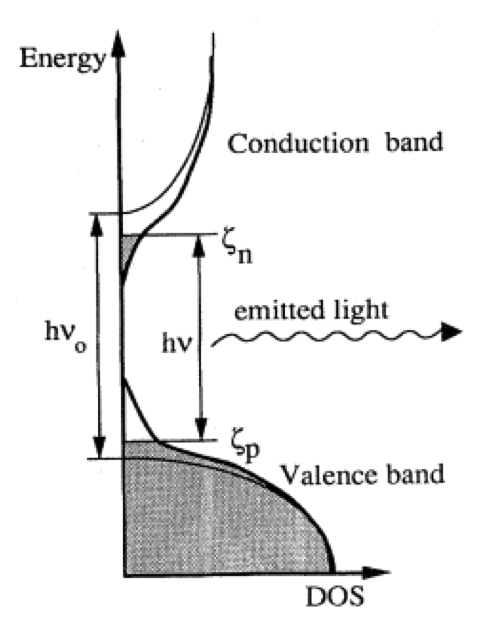
\includegraphics[width=0.4\textwidth]{figures/pankove_band_tailing.png}
%    \caption{Schematic of the laser operation at T=0 K in GaAs. $\zeta_{n,p}$ are the quasi-Fermi level for electrons and holes respectively. The narrow line denotes the unperturbed density of states (DOS), while the heavy line depicts the DOS modified by heavy-doping effects. Both valence and conduction bands are shifted towards each other to give a narrowing of the band gap and the DOS is distorted, showing band tails. Heavy doping effects result in a different emitted spectrum. Figure taken from reference \citenum{Pankove}. **CONDENSE FIGURES**}
%  \label{pankove_band_tailing}
%\end{figure}

 



\chapter{Methodology}

\section{Electronic structure calculations}\label{elec_struc}
%See Richard Martin book (Ch1), etc. \cite{RichardMartin_Ch1}

\subsection{Quantum theory of materials}

%** See Prasad ch1 (intro) + ch2 for SE\\

The properties of materials are determined by their constituent electrons and nuclei and how they interact with each other. Nuclei are massive (compared to electrons) and can usually be described using classical mechanics with interactions via Coulomb's law. However, as hypothesised by de Broglie in 1924 and later demonstrated experimentally by Davisson and Germer and also by Thomson with electron diffraction, electrons exhibit wave-like behavior in addition to particle-like behavior and do not obey classical mechanics \cite{quantum_intro}. The behaviour of the electrons largely determines the physical and chemical properties of a material \cite{Prasad_ch2}, such as the bonding that holds the material together and many of the observed macroscopic properties such as the optical, electrical and magnetic properties \cite{RichardMartin_Ch1}. To describe the behaviour of electrons, it is necessary to use quantum mechanics.

Quantum mechanical systems can be described by the Schr{\"o}dinger equation (SE), which can describe the energy of the electrons and nuclei within a material where electrons interact with the positively charged atomic nuclei through an electrostatic potential \cite{Lesar}. The time-dependent SE for a one-electron system is given in Eq.~\ref{SE}, where the first term on the left hand side of the equation is related to the electron's kinetic energy, the second term to the electron's potential energy ($\hat{V}$) and $\psi$ is used to denote the one-electron wavefunction.
\begin{equation} \label{SE}
\left( - \frac{\hbar^2}{2m} \nabla^2 + \hat{V} \right)\psi(r,t) = i\text{ } \hbar\frac{\partial \psi(r,t)}{\partial t}
\end{equation}
%In section \ref{BandTheorySection} the one-electron Schr{\"o}dinger equation for an electron moving in a weak periodic potential with the nearly free electron approximation was used to discuss obtaining the energy eigenvalues of the electron as a function of \textbf{k}, i.e. the electronic band structure of a periodic, crystalline solid.
%However, 
For systems containing more than one electron we must consider the many-body SE and this soon becomes a very complex problem. This is due to the many electrons in the system interacting with each other as well as with the nuclei. The SE for a system containing M nuclei and N electrons is shown in Eq.~\ref{many_SE} \cite{Lesar}, where uppercase \textbf{R} denotes nuclear coordinates and lowercase \textbf{r} denotes electron coordinates. This is a very complex mathematical problem for most systems. For example, the many-body wavefunction, $\Psi$, in Eq.~\ref{many_SE} for 1 cm$^3$ of a typical metal would be a function of approximately $10^{23}$ variables.

\begin{multline}  \label{many_SE}
\left\{ - \frac{\hbar^2}{2m} \left( \frac{\nabla_{n_1}^2}{m_1} + ... + \frac{\nabla_{n_M}^2}{m_M}, 
\frac{\nabla_{e_1}^2}{m_e} + ... + \frac{\nabla_{e_N}^2}{m_e} \right)
+ V \left( \mathbf{R_1},...,\mathbf{R_M}, \mathbf{r_1}, ..., \mathbf{r_N} \right)
\right\} \\
\Psi (\mathbf{R_1},...,\mathbf{R_M}, \mathbf{r_1}, ..., \mathbf{r_N}, t)
= i\hbar \frac{\partial\Psi(\mathbf{R_1},...,\mathbf{R_M}, \mathbf{r_1}, ..., \mathbf{r_N},t)}{\partial t}
\end{multline}

When dealing with such systems, the Born-Oppenheimer approximation is almost universally used. As electrons are fast moving relative to the nuclei, they are considered to be moving in the classical field generated by static nuclei. This approximation decouples the nuclear and electronic degrees of freedom, allowing us to separate the ionic and electronic wavefunctions. 
%The total energy of the system is now just the sum of the energy of the electrons and the nuclei and only the electronic density requires quantum mechanical treatment. 
When using the Born-Oppenheimer approximation it is also assumed that nuclear motion cannot cause electronic transitions, therefore the electrons will remain in their ground state. There is now no explicit time dependence for the electron density as electrons are assumed to always be in their ground state for the instantaneous ionic configuration and that they transition adiabatically to their ground state for each ionic configuration. This approximation is generally more suitable for semiconductors than for metals as phonon energies are usually less than the energy of the electronic band gap in a semiconductor and hence ionic motion cannot excite electrons to higher energy states \cite{Prasad_ch2}. $\Psi$ for electrons in the system is now no longer a function of t and so it is the solution of the time-independent SE for the system of ions and electrons that is of interest and the ionic system can be considered separately from the electronic system which is subjected to the classical electric field of a stationary ionic system.
%and is only a function of electron coordinates (lowercase r in Eq. \ref{many_SE}).

The general form of a time-independent SE for the electronic system is shown in Eq.~\ref{TISE}, where $\hat{H}$ is the Hamiltonian operator used to determine the total energy of a system with the wavefunction $\Psi$. Lowercase \textbf{r} are the electronic coordinates and $\sigma$ is used to denote the spin of electrons, which was omitted in earlier equations for simplicity. The Born-Oppenheimer Hamiltonian for the electrons is shown in Eq.~\ref{Born-Opp}, where l are the ionic sites, Z is the nuclear charge, m is the electron mass, i is the index of the electron and j are the indices of all other electrons in the system. The first term is the kinetic energy of the electrons, the next terms are related to the potential energy of the electrons. The second term is the Coulomb attraction between electrons and static nuclei and the third term is the Coulomb repulsion between different electrons \cite{Prasad_ch2}.
\begin{equation}\label{TISE}
\hat{H}\Psi(\mathbf{r_1}, ..., \mathbf{r_N}, \sigma_1, ..., \sigma_N) = E\Psi(\mathbf{r_1}, ..., \mathbf{r_N}, \sigma_1, ..., \sigma_N)
\end{equation}
\begin{equation}\label{Born-Opp}
\hat{H} = - \sum_i \frac{\hbar^2}{2m}\nabla_i^2 - \frac{1}{4 \pi \epsilon_0}\sum_i \sum_l \frac{Ze^2}{|\mathbf{r_i}-\mathbf{R_l}|} + \frac{1}{8 \pi \epsilon_0} \sum_{ij, i \neq j}\frac{e^2}{|\mathbf{r_i}-\mathbf{r_j}|}
\end{equation}
Although we can write out the electron Hamiltonian as shown above, we do not know the exact form of the many-body wavefunction in Eq.~\ref{TISE}. The third term in the expression for the Hamiltonian, the summation of electron-electron interactions in the system, is the cause of a dramatic rise in computational expense as the system size (and hence number of interacting electrons) increases. In the next section some of the various approaches that have been developed to treat electron-electron interactions are outlined and those utilised in this work are highlighted.

%\subsection{History of electronic structure theory}

\subsection{Treatments of electron-electron interactions}

\subsubsection{Approximations of the many-body wavefunction}
As we do not know the exact form of the many-body wavefunction, $\Psi$, the simplest way to avoid the dramatic rise in complexity in the many-body SE from electron-electron interactions with increased system size is to approximate the form of $\Psi$ in a manner that allows us to decouple electron-electron interactions. In the `independent particle approximation', as used in the Hartree method, electrons are treated as independent and are included in an average electron-electron interaction scheme. The method involves assuming approximate forms of both the Hamiltonian and the many-body wavefunction. The electron-electron interaction term in the Hamiltonian in Eq. \ref{Born-Opp} is replaced by one that accounts for only the repulsion between an electron and the average position of all other electrons, the electrons therefore interact with an average effective potential instead of many, many interactions between all pairs of electrons in the system. This is an example of a mean field approximation.
%The second term in  Eq. \ref{Born-Opp} is then combined with the modified electron-electron interaction term to form an effective potential, the Hartree potential (V$_{eff}$). 
As electrons are considered to be independent, the many-body wavefunction can be written as the product of single-electron wavefunctions (or orbitals) as shown in Eq.~\ref{Hartree}, where $\psi_i(\mathbf{r_i}, \sigma_i)$ is the wavefunction of a single electron i at position $r_i$ with spin $\sigma_i$ \cite{Prasad_ch2}. 
\begin{equation}\label{Hartree}
\Psi_H = \psi_1(\mathbf{r_1}, \sigma_1) \psi_2(\mathbf{r_2}, \sigma_2) ... \psi_N(\mathbf{r_N}, \sigma_N)
\end{equation}
To solve the many-body SE, the Hartree method pioneered the self-consistent field method \cite{RichardMartin_Ch1}. Firstly, the variational principle is invoked to set up an inequality for the groundstate energy, $E_0$, of the system (i.e. the minimum total energy) to find an approximate value of $E_0$ and the corresponding set of $\psi_i$. This is shown in Eq.~\ref{var_princip} where the middle term is the expectation value of a state of the system described by the many-body wavefunction $\Psi$. Many properties of interest can be determined from $E_0$ of the system and from changes in the energy of the system in response to particular perturbations. $E_0$ can be used to determine various structural properties such as equilibrium bond lengths, surface configurations and the most likely defect structures in a material.
\begin{equation}\label{var_princip}
E = \braket{\Psi | \hat{H} | \Psi } \geq E_0
\end{equation}
The solution of the Hartree equation, shown in Eq.~\ref{Hartree_eq}, depends on the Hartree potential, shown in Eq.~\ref{V_Hartree}, but the potential depends on the solution of the Hartree equation itself to obtain $\psi_i$. The solution of the Hartree equation therefore involves a self-consistent procedure. A guess is made for $V_H(\mathbf{r})$ and then Eq.~\ref{Hartree_eq} is solved. Then the solution is used to calculate $V_H(\mathbf{r})$ with Eq. \ref{V_Hartree} and the Hartree equation is solved again with this new value for $V_H(\mathbf{r})$. The procedure is repeated until input and output potentials are the same, within a specified tolerance \cite{Prasad_ch2}.
\begin{equation}\label{Hartree_eq}
\left[ -\frac{\hbar^2}{2m_e}\nabla^2 + V_I(\mathbf{r}) + V_H(\mathbf{r}) \right] \psi_i(\mathbf{r}) = \epsilon_i \psi_i(\mathbf{r})
\end{equation}
\begin{equation}\label{V_Hartree}
V_H(\mathbf{r_i}) = \frac{1}{4 \pi \epsilon_0} \sum_{j \neq i} \int \frac{ e^2 |\psi_j|^2}{|\mathbf{r_i} - \mathbf{r_j}|}  d^3r_j
\end{equation}
\begin{equation}\label{V_I}
V_I(\mathbf{r_i}) = -\frac{1}{4 \pi \epsilon_0} \sum_l \frac{Ze^2}{|\mathbf{r_i} - \mathbf{R_l}|}
\end{equation}

There are a number of large drawbacks of the Hartree method. The mean-field approach to obtaining the Hartree potential is flawed due to spurious self-interactions. 
As every electron is included in the average electron density, when calculating the electron-electron interaction term each electron will also be interacting with itself.
The next large omission of the Hartree method is electron correlation. The probability of finding an electron at $\mathbf{r_1}$ is uncorrelated to finding one at $\mathbf{r_2}$ because it can be written as a product of two one-electron probabilities. Paraphrasing John Perdew from his talk at the 2015 `Hands-on workshop density-functional theory and beyond: First-principles simulations of molecules and materials' helps to explain why this is neglecting some behaviour of the electron density: electron correlation can be likened to shoppers at a busy shopping mall where many people are moving around but in such a way that they try to avoid bumping into each other. Neglecting this effect can lead to results as unphysical as the dissociation of the H$_2$ molecule \cite{Prasad_ch2}.

Lastly, the basic Hartree method described above does not account for electron exchange. Although the spin of the electron is included in Eq.~\ref{Hartree}, it actually plays no role in the Hartree method. The many-body wavefunction needs to be antisymmetric under particle exchange as required by the Pauli Exclusion Principle for fermions. This requirement is shown in Eq.~\ref{antisym}. According to the Pauli Exclusion Principle, no two fermions can occupy the same quantum state. The spin quantum number therefore should be taken into account. The Hartree-Fock (H-F) extension to this method is able to account for this latter flaw \cite{Prasad_ch2}.
\begin{equation}\label{antisym}
\Psi(\mathbf{r_1}\sigma_1, ..., \mathbf{r_i}\sigma_i, ..., \mathbf{r_j}\sigma_j, ...) = - \Psi(\mathbf{r_1}\sigma_1, ..., \mathbf{r_j}\sigma_j, ..., \mathbf{r_i}\sigma_i, ...)
\end{equation}
The requirement shown in Eq.~\ref{antisym} can be satisfied by using the Slater determinant as the trial wavefunction, as shown in Eq.~\ref{Slater_det}, where N is the number of electrons.
\begin{equation}\label{Slater_det}
\Psi(\mathbf{r_1}\sigma_1, ..., \mathbf{r_N}\sigma_N) = \frac{1}{\sqrt{N!}} \begin{bmatrix}
\psi_1(\mathbf{r_1}\sigma_1) & \psi_1(\mathbf{r_2}\sigma_2) & \dots & \psi_1(\mathbf{r_N}\sigma_N) \\
\psi_2(\mathbf{r_1}\sigma_1) & \psi_2(\mathbf{r_2}\sigma_2) & \dots & \psi_2(\mathbf{r_N}\sigma_N) \\
\vdots & \vdots & \vdots & \vdots \\
\psi_N(\mathbf{r_1}\sigma_1) & \psi_N(\mathbf{r_2}\sigma_2) & \dots & \psi_N(\mathbf{r_N}\sigma_N) 
\end{bmatrix}
\end{equation}
When using the Slater determinant as the trial wavefunction, each electron is now surrounded by an `exchange hole' in which the probability of finding another electron is very small. The exchange term in the H-F method also cancels the self-interaction in the Hartree potential as a result of the antisymmetry.
%The exchange interaction is a real quantum mechanical effect and must appear in any one-electron model. The H-F method, like the Hartree method, is a mean-field theory and hence the many-body problem is reduced to a one-electron problem where the electron moves in an average field generated by the other electrons \cite{Prasad_ch2}. 
However, the H-F method still neglects Coulomb repulsion correlation effects that arise due to electrons moving in such a way to avoid each other. It includes some correlation effects between parallel spin electrons from the explicit treatment of exchange interactions, but neglects correlations between opposite spin electrons. 
The exchange term tends to lower the total energy of the system due to the tendency to keep two electrons with the same spin apart, however, the Coulomb correlations reduce the exchange interaction between electrons with parallel spins, so the H-F method overestimates the strength of the exchange interaction. The H-F method is better suited to compact systems such as atoms or molecules but describes conduction electrons in solids poorly \cite{Prasad_ch2} and, despite the approximations used, is still very computationally demanding \cite{Prasad_ch1}.
%$\Psi(3N)$ where n is the number of electrons 

Coulomb correlations can be introduced by using the Configuration Interaction method which involves writing the many-body wavefunction as a weighted sum of H-F wavefunctions for different electronic configurations. This method has been successful for atoms and molecules, but is very difficult to apply for large molecules or solids \cite{Prasad_ch2} and is therefore not used at all in this work where calculations have only been performed for solid-state systems. For solids, density functional theory (DFT) is usually the methodology of choice, which is outlined in the next section.


%\subsubsection{Density functional theory (DFT)}
\subsubsection{Electron density methods}

The essence of density functional theory (DFT) is to write the total energy as functional of a simpler quantity to provide a more feasible approach to solving the many-body Schr{\"o}dinger equation. The methods described above solve the many-body Schr{\"o}dinger equation by approximating the many-body wavefunction, $\Psi$, which involves the coordinates of all electrons in the system and therefore is a function of 3N variables, where N is the number of electrons in the system which is typically large for most systems of interest. If the system is instead described by the electron density, n(\textbf{r}), instead of $\Psi$ the key quantity in the equation would instead be a function of 3 variables \cite{Prasad_ch3}.

The earliest electron density method was the Thomas-Fermi theory proposed in 1927 \cite{Thomas-Fermi_1, Thomas-Fermi_2}. In the original method, the kinetic energy of the system is approximated as an explicit functional of the electron density, simplified to a non-interacting homogeneous electron gas with density equal to the local density at any given point.
However, approximations used in this method are too crude to account for many essential physical and chemical aspects of matter, such as the electronic shell structures of atoms and the binding of molecules \cite{RichardMartin_Ch6}.

In 1964 Hohenberg and Kohn provided two theorems (and corresponding proofs) which formulated DFT as an exact theory of many-body systems \cite{hohenberg_kohn1964}. The ansatz provided by Kohn and Sham a year later \cite{Kohn_Sham1965} then allowed for the construction of useful, approximate ground state functionals for real systems of many electrons. The two Hohenberg-Kohn theorems are as follows:
\begin{enumerate}
\item The external potential, $V_{ext}(\mathbf{r})$, of a system of interacting electrons in an external potential, $V_{ext}(\mathbf{r})$, is a unique functional of the ground state electron density, $n(\mathbf{r})$. The total ground state energy, E, of a many-electron system therefore is also a unique functional of $n(\mathbf{r})$, E[n(\textbf{r})].
\item The total energy functional, E[n(\textbf{r})], for the total energy has a minimum equal to the ground state energy at the ground state electron density. 
\end{enumerate}
Combining both Hohenberg-Kohn theorems says that the ground state energy of a system can be determined from the unique ground state electron density by minimising the energy functional, E[n(\textbf{r})], with respect to the electron density, n(\textbf{r}). However, this does not yet tell us anything about the form of E[n(\textbf{r})]. 

The approach proposed by Kohn and Sham in 1965 involves replacing the original interacting many-body problem by an auxiliary system that can be solved more easily. This auxiliary system involves independent electrons, but an interacting density. The assumption made here is that the ground state density of the original interacting system is the same as that of some auxiliary non-interacting system, where all complex many-body interaction are incorporated into an exchange-correlation functional of the electron density, $E_{xc}[n(\mathbf{r})]$. When the Kohn-Sham equations are solved, the ground state electron density of the original system is then determined, with accuracy limited only by the approximate form of $E_{xc}[n(\mathbf{r})]$ \cite{RichardMartin_Ch7}.

Using the Born-Oppenheimer approximation, E[n(\textbf{r})] can be expressed as shown in Eq.~\ref{E_functional} where the first term is the external potential from the interaction between electrons and nuclei and the second term is usually denoted as F[n(\textbf{r})]. This term is a functional of the electrons only where T is the functional for the electron kinetic energy and $V_{EE}$ is for electron-electron interactions.
\begin{equation}\label{E_functional}
E[n(\mathbf{r})] = \braket{\Psi | V_{ext} | \Psi} +  \braket{\Psi | T + V_{EE} | \Psi} = \braket{\Psi | V_{ext} | \Psi} + F[n(\mathbf{r})]
\end{equation}
F[n(\textbf{r})] can be split into three parts as shown in Eq.~\ref{F_functional} where $T[n(\mathbf{r})]$ is the kinetic energy of a non-interacting electron gas of density $n(\mathbf{r})$ in its ground state, the second term is the classical Coulomb repulsion energy between the electrons and the last term then contains all of the many-body effects of the electronic system, including: exchange, correlation and part of the total kinetic energy \cite{Prasad_ch3}.
\begin{equation}\label{F_functional}
F[n(\mathbf{r})] = T[n(\mathbf{r})] + \frac{e^2}{2}\int \int \frac{1}{4\pi \epsilon_0}\frac{n(\mathbf{r})n(\mathbf{r^{\prime}})}{|\mathbf{r} - \mathbf{r^{\prime}}|}d^3rd^3r^{\prime} + E_{xc}[n(\mathbf{r})]
\end{equation}
Substituting Eq.~\ref{F_functional} into Eq.~\ref{E_functional}, Eq.~\ref{E_functional} can be re-written as shown in Eq.~\ref{E_functional_2}. If Eq.~\ref{E_functional_2} is minimised subject to the constraint that the integral of the electron density over the whole system volume is equal to the number of electrons in the system (Eq.~\ref{n_constraint}), this gives Eq.~\ref{E_func_min}, where the third term is the Hartree potential ($V_H$), the fourth term is the exchange-correlation potential ($V_{xc}$) and the fifth term is the Lagrange multiplier.
\begin{equation}\label{E_functional_2}
E[n(\mathbf{r})] = \int V_{ext}(\mathbf{r})n(\mathbf{r})d^3r + T[n(\mathbf{r})] + \frac{e^2}{2}\int \int \frac{1}{4\pi \epsilon_0}\frac{n(\mathbf{r})n(\mathbf{r^{\prime}})}{|\mathbf{r} - \mathbf{r^{\prime}}|}d^3rd^3r^{\prime} + E_{xc}[n(\mathbf{r})]
\end{equation}
\begin{equation}\label{n_constraint}
\int n(\mathbf{r})d^3r = N
\end{equation}
\begin{equation}\label{E_func_min}
\frac{\partial T[n(\mathbf{r})]}{\partial n(\mathbf{r})} + V_{ext}(\mathbf{r}) + \int \frac{e^2}{4\pi \epsilon_0}\frac{n(\mathbf{r^{\prime}})}{|(\mathbf{r})-(\mathbf{r^{\prime}})|}d^3\mathbf{r^{\prime}} + \frac{\partial E_{xc}[n(\mathbf{r})]}{\partial n(\mathbf{r})} - \mu = 0
\end{equation}
Kohn and Sham noted that, apart from the inclusion of E[n(\textbf{r})], Eq.~\ref{E_functional} is identical to Hartree's expression for energy. Without the corresponding term in Eq.~\ref{E_func_min}, $V_{ext}(\mathbf{r})$, this could be solved in a similar manner to the Hartree method by using the substitution in Eq.~\ref{n_wavefunc} and solving Eq.~\ref{KS_Hartree}.
\begin{equation}\label{n_wavefunc}
n(\mathbf{r}) = \sum^N_{i=1} |\psi_i(\mathbf{r})|^2
\end{equation}
\begin{equation}\label{KS_Hartree}
\left( -\frac{\hbar^2}{2m_e}\nabla^2 + V_{ext}(\mathbf{r}) + V_H(\mathbf{r}) \right) \Psi_i(\mathbf{r}) = \epsilon_i \Psi_i(\mathbf{r})  
\end{equation}
If n(\textbf{r}) can be defined in terms of one-electron orbitals as in Eq.~\ref{n_wavefunc} but by also including $V_{xc}(\mathbf{r})$ through an effective potential, $V_{eff}(\mathbf{r})$, as shown in Eq.~\ref{KS_pot}, then the Kohn-Sham (KS) equations shown in Eq.~\ref{KS_eq} can be solved self-consistently, analogously to solving Eq.~\ref{KS_Hartree} in the Hartree method.
\begin{equation}\label{KS_pot}
V_{eff}(\mathbf{r}) = V_{ext}(\mathbf{r}) + V_H(\mathbf{r}) + V_{xc}(\mathbf{r})
\end{equation}
\begin{equation}\label{KS_eq}
\left( -\frac{\hbar^2}{2m_e}\nabla^2 + V_{eff}(\mathbf{r}) \right) \Psi_i(\mathbf{r}) = \epsilon_i \Psi_i(\mathbf{r})
\end{equation}
The set of fictitious, non-interacting one-electron wavefunctions in Eq.~\ref{n_wavefunc} are called the KS orbitals. However, these do not correspond to the physical atomic orbitals of the system. The KS orbitals are used to reproduce the correct ground state electron density when mapping the interacting electron system onto an auxiliary system of independent particles, which move in the KS potential from Eq.~\ref{KS_pot}. Although solving Eq.~\ref{KS_eq} is very similar to the Hartree method and reduces the many-electron problem to a set of one-electron problems, unlike the Hartree or H-F methods, DFT includes the effects of electron correlations as well as exchange because of the $V_{xc}(\mathbf{r})$ term. While the H-F method treats exchange exactly, it neglects correlations completely. The form of $V_{xc}(\mathbf{r})$ is not known therefore some approximation has to be made for this function. Exchange and correlation are both included in DFT, but only approximately. However, reasonable accuracy has been achieved with these approximate forms \cite{Prasad_ch3}. In the next section common approximations used in DFT will be outlined and those utilised in this work will be highlighted.

%Starting point: http://iopscience.iop.org/article/10.1238/Physica.Topical.109a00009/pdf
%(Good for original citations!)



\subsubsection{Exchange-correlation functionals, $E_{xc}[n(\textbf{r})]$}
In 1965 Kohn and Sham also developed the first approximate form for the exchange-correlation functional, the local density approximation (LDA). Due to the explicit separation of the independent particle kinetic energy and long-ranged Hartree terms in Eq.~\ref{E_functional_2}, the remaining exchange-correlation energy contributions can be approximated by a local or nearly-local functional of the electron density \cite{RichardMartin_Ch7}. In this approximation, it is assumed that the electron density, n(\textbf{r}), varies very slowly in space such that the electron gas in a small volume could be considered as approximately uniform locally, close to the limit of the homogeneous electron gas (HEG) \cite{RichardMartin_Ch8}. This approximation would then allow for the use of the exchange-correlation energy of the HEG to evaluate the form of the exchange-correlation functional, as shown in Eq.~\ref{LDA_E_func} where $\epsilon_{xc}(n)$ is the exchange-correlation energy per particle of a uniform gas of density n(\textbf{r}) \cite{Prasad_ch3}. A simple analytic form is known for the exchange energy of the HEG and the correlation energy of the HEG has been calculated using Monte Carlo methods in Ref.~\citenum{LDA_HEG} \cite{RichardMartin_Ch8}.
\begin{equation}\label{LDA_E_func}
E_{xc}[n(\mathbf{r})] = \int \epsilon_{xc}(n(\mathbf{r}))n(\mathbf{r})d^3r
\end{equation}
This approach can also be extended to spin-polarised systems with the localised spin density approximation (LSDA) where there is an unequal number of spin-up and spin-down electrons. In this case, $E_{xc}[n(\mathbf{r})]$ is split into separate parts for the spin-up and spin-down electron densities \cite{Prasad_ch3}.

Although the LDA has given remarkably good results for some systems, such as simple metals where the electron density more closely resembles the HEG, performance is poorer for more inhomogeneous systems, like atoms where the density must continuously approach zero outside of the atom \cite{RichardMartin_Ch8}. The accuracy of the LDA is not sufficient for purposes such as predicting binding energies for chemical reactions, subsequent works therefore have sought to construct improved functionals. 
The gradient expansion approximation (GEA) was suggested by Kohn and Sham \cite{Kohn_Sham1965} where $E_{xc}[n(\mathbf{r})]$ is expanded in terms of gradients of the electron density in Taylor series and truncated at some order \cite{Prasad_ch3}.
%magnitude of the gradient of the electron density at each point is considered, as well as the density, when creating the functional. 
The exact exchange-correlation energy is related to the concept of an `exchange-correlation hole' in which all other electrons are excluded. The integration over this hole in the electron density is equal to one electron, hence the combination of the electron and the exchange-correlation hole gives a net neutral unit. The LDA approximates the exchange-correlation hole to be a sphere, while the inclusion of gradients in the electron density allows for more elaborate shapes for the exchange-correlation hole \cite{RichardMartin_Ch7}.
%These functionals aim to improve on the assumption made in the LDA that the electron density varies very slowly in space by including not just the electron density at a given location, but also the gradient in the density when approximating $E_{xc}[n(\textbf{r})]$ \cite{Prasad_ch3}.

However, the GEA was not found to give systematic improvements over the LDA and important conditions such as the sum rules for the exchange-correlation holes were violated. The large density gradients in real materials cause the low-order gradient expansions to break down. 
Generalised-gradient expansions (GGAs) have been proposed instead.
Here functionals are constructed that are functions of both electron density, $n(\mathbf{r})$, and gradients in the density, $\nabla n(\mathbf{r})$, which do satisfy sum rules. The general, spin-polarised form of a GGA is shown in Eq.~\ref{GGA}. Various functions are used for $f$ in the equation and $n_{\uparrow}(\mathbf{r})$ and $n_{\downarrow}(\mathbf{r})$ correspond to the density of spin up and spin down electrons respectively.
Various GGAs have been developed to improve the predictive power of DFT and have demonstrated sufficient accuracy to now be utilised by the chemistry community.
The rapidly varying electron density in atoms leads to a greater lowering of exchange energy in atoms and molecules than in solids, this results in a reduction in the binding energy which is not accounted for by the LDA. The use of density gradients in the GGA is able to correct for some of the overbinding from the LDA \cite{RichardMartin_Ch8}. 

%** Add in general GGA from Prasad pg 61 Eq. 3.52 + GEA as truncated gradient density as Taylor expansion but GGA constructs functional of electron density without using such expansion method?? **

\begin{equation}\label{GGA}
E_{xc}^{GGA}[ n_{\uparrow}(\mathbf{r}), n_{\downarrow}(\mathbf{r})] = \int d^3r f [ n_{\uparrow}(\mathbf{r}), n_{\downarrow}(\mathbf{r}), \nabla n_{\uparrow}(\mathbf{r}), \nabla n_{\downarrow}(\mathbf{r})]
\end{equation}

Some GGA functionals are semi-empirical due to their use of fits to experimental data. An example of one of the less empirical functionals is the PBE functional \cite{PBE}, where the main parameterisation is in the LDA component and otherwise fundamental physical constants are favoured over empirical fits.
Semi-empirical GGAs can accurately represent small molecules, but usually fail for delocalised electrons in the uniform gas or for simple metals. First-principles numerical GGAs can be constructed from electron density-gradient expansions for the exchange-correlation hole surrounding the electron in a system of slowly varying density with spurious long-range terms cut off to satisfy sum rules on the exact hole \cite{PBE}.
However, accurate atomic exchange energies require violating the gradient expansion for slowly varying densities, which are more appropriate when modelling solids. A gradient expansion that works well for an atomic system is likely to perform poorly for a solid. For this reason, an alternative PBE functional has been developed for solids, the PBEsol functional \cite{PBEsol}. In this work, the PBEsol functional is often used for obtaining geometries. However, there are still some shortcomings in the simulation of semiconductors for PV applications with semilocal functionals such as PBEsol. A notable issue is the band gap error where the electronic band gap of semiconductors and insulators is often substantially underestimated compared to experimental measurements \cite{band_gap_error}. Significant improvements in the computational prediction of this important material property have been achieved with some `beyond-DFT' methods. One method for this, which is utilised in this work, is hybrid density functionals which are introduced in the next section.

%** Check over and condense GGA section + look up sum rule again (xc hole – sum of wavefunc*occ no. must equal -1? + look into LDA/ GGA overbinding vs. underbinding?? **

%+ Richard Martin Ch6-9. 6 for DFT fundamentals, e.g. Hohenberg and Kohn theorems for simple existence proof of functionals but no guidance on form \cite{RichardMartin_Ch6}, 7 for Kohn-Sham ansatz (way to make useful, approximate ground state functionals for real systems of many electrons) \cite{RichardMartin_Ch7}, 8 for common approximations for xc functionals \cite{RichardMartin_Ch8}, 9 for solution of Kohn-Sham independent particle approximations \cite{RichardMartin_Ch9}

\subsubsection{Hybrid-DFT}\label{hse_theory}
Various hybrid density functionals have been developed to improve upon standard DFT. One such approach is to incorporate some exact, non-local H-F exchange into a pure GGA functional. The exchange component, x, of this hybrid exchange-correlation functional, $E_{xc}^{hybrid}[n(\mathbf{r})]$, is expressed as a linear combination of the exchange components of the DFT functional, $E_{xc}^{DFT}[n(\mathbf{r})]$, and the H-F functional, $E_{xc}^{HF}[n(\mathbf{r})]$, with some mixing parameter a, as shown in Eq.~\ref{hybrid_Exc}.
\begin{equation}\label{hybrid_Exc}
E_{xc}^{hybrid}[n(\mathbf{r})] = E_{xc}^{DFT}[n(\mathbf{r})] + a(E_{x}^{HF}[n(\mathbf{r})] - E_{x}^{DFT}[n(\mathbf{r})])
\end{equation}
The H-F method tends to underbind atoms in molecules \cite{DFT_delocalisation}. Although electron exchange is treated exactly, the method completely neglects electron correlation and therefore the modelled system entirely lacks a mechanism by which the electron arrangement could act to lower the total energy of the system. Hence the total energy of the system may be overestimated. DFT however, in particular the LDA, overbinds atoms in molecules and overly favours the formation of bonds \cite{DFT_delocalisation}. The approximation of a more uniform electron density than what may exist in the system in reality when constructing such electron density functionals may result in the assumption of a stronger, more uniform bonding arrangement, artificially lowering the total energy of the system. Some types of hybrid density functionals have been constructed to improve upon both methods by combining them, but the ways in which the functionals are combined differs for different hybrid functionals.

In this work, the HSE06 hybrid functional \cite{HSE2} is frequently used for calculations of electronic properties. This functional has been demonstrated to produce accurate electronic properties with predicted electronic band gaps for semiconductors much closer to experimental values than those produced using semilocal functionals such as PBE and PBEsol \cite{HSEsol}.
The HSE06 functional involves two adjustable parameters. Firstly, the mixing parameter a, as in Eq.~\ref{hybrid_Exc}, but also a parameter $\omega$ which determines the screening of the exact exchange in the construction of this functional. 
The HSE06 functional uses PBE as the GGA functional, incorporates 25\% H-F exchange (with a=$\frac{1}{4}$) and uses $\omega$ = 0.11 bohr$^{-1}$ for the screening parameter \cite{HSE2}.

The exact H-F exchange is very computationally expensive to calculate for large molecules and solids. Kohn has shown that the range of the exchange interaction in insulators decays exponentially as a function of the band gap \cite{HSE_ref13}. Therefore, convergence with distance is very slow for small gap or metallic systems \cite{HSE}.
Screened hybrid functionals, such as the HSE06 functional, have been introduced to reduce the computational expense of the inclusion of exact H-F exchange. In the case of the HSE06 functional, a screened Coulomb potential is applied to the exchange interaction only to screen the long-range component of the H-F exchange \cite{HSE2}. This restricts the Fock exchange calculations to small electron-electron separations \cite{HSE_systematic}. The Coulomb operator is split into short-range (SR) and long-range (LR) components as shown in Eq.~\ref{HSE_SR_LR} in the first and second terms on the right-hand side of the equation respectively and $\omega$ defines the separation range.
\begin{equation}\label{HSE_SR_LR}
\frac{1}{r} = \frac{erfc(\omega r)}{r} + \frac{erf(\omega r)}{r}
\end{equation}
All of the terms for the hybrid exchange energy are split into their short- and long-ranged components in Eq.~\ref{Ex_SR_LR}.
\begin{equation}\label{Ex_SR_LR}
E_x^{hybrid} = aE_x^{HF,SR}(\omega) + aE_x^{HF,LR}(\omega) + (1-a)E_x^{PBE,SR}(\omega) + E_x^{PBE,LR}(\omega) - aE_x^{PBE,LR}(\omega)
\end{equation}
Numerical tests indicated that the LR H-F and PBE exchange contributions to this functional are small and tend to cancel each other \cite{HSE}, therefore these terms are neglected in the expression for the exchange-correlation energy in Eq.~\ref{HSE06}.
\begin{equation}\label{HSE06}
E_{xc}^{HSE06} = aE_x^{HF,SR}(\omega) + (1-a)E_x^{PBE,SR}(\omega) + E_x^{PBE,LR}(\omega) + E_c^{PBE}
\end{equation}
When the adjustable parameter $\omega = 0$, the LR term becomes zero and the SR term is the full Coulomb operator, equivalent to an unscreened hybrid functional. When $\omega \rightarrow \infty $, the HSE functional becomes identical with the semilocal PBE functional. The values chosen for a and $\omega$ in the HSE06 functional have been found to be close to the optimum in terms of accuracy and computational efficiency in a systematic study varying these parameters in hybrid functionals \cite{HSE_systematic}. However, the study also identifies alternative values for the two parameters for improved accuracy over the HSE06 functional and also parameters which were found to match the accuracy of the HSE06 functional but with reduced screening length and hence reduced computational expense. Improvement in the accuracy and transferability of density functionals to various systems is an on going area of research.

%This functional has been demonstrated to produce good band gaps... Adam thesis ref 25 (study on a and $\omega$ sensitivity for predicting Eg of semiconductors, HSE06 params v close to optimal values found to outperform hybrid unscreened functional PBE0. \cite{HSE_systematic}


\subsection{Implementation for periodic solids}

Concepts for the theoretical modelling of periodic solids were outlined in section \ref{crystal_models}. The use of Bloch's theorem to account for the effect of a periodic lattice potential on a state described by a single-electron wavefunction was outlined in section \ref{BandTheorySection}. Electronic structure calculations performed in this work are for periodic solids and therefore make use of 3D periodic boundary conditions (PBCs) to simulate infinite, bulk solids using only a unit cell of the crystal. The only deviations from the basic implementation of PBCs are in section \ref{sulfosalt_band_alignment}. This work involved calculating surface properties of candidate solar absorber materials to investigate possible candidate solar cell heterojunction partners. Methodology for this study will be outlined in section \ref{band_alignment_methods}. The other deviation from simple PBCs for electronic structure calculations in this work is the simulation of point defects in the dilute limit using the supercell method \cite{SupercellMethodDefects}. This method will be discussed further in section \ref{defects_methods}. 

In the rest of this section, approaches used in this work for electronic structure calculations of periodic solid-state systems will be outlined with comments on their relative merits for chemical accuracy and computational efficiency. Representations of the wavefunction in different electronic structure software packages that are used in this work will first be described. Then the general workflow for geometric and electronic optimisation will be outlined. The section concludes with a discussion of determining the most appropriate setup for electronic structure calculations in terms of an optimal compromise between chemical accuracy and computational efficiency.

%Offline sources for flight: VASP slides, FHI-aims slides + RM ch4 + theses


\subsubsection{Representations of wavefunctions for electronic structure calculations}
\begin{figure}[h!]
  \centering
    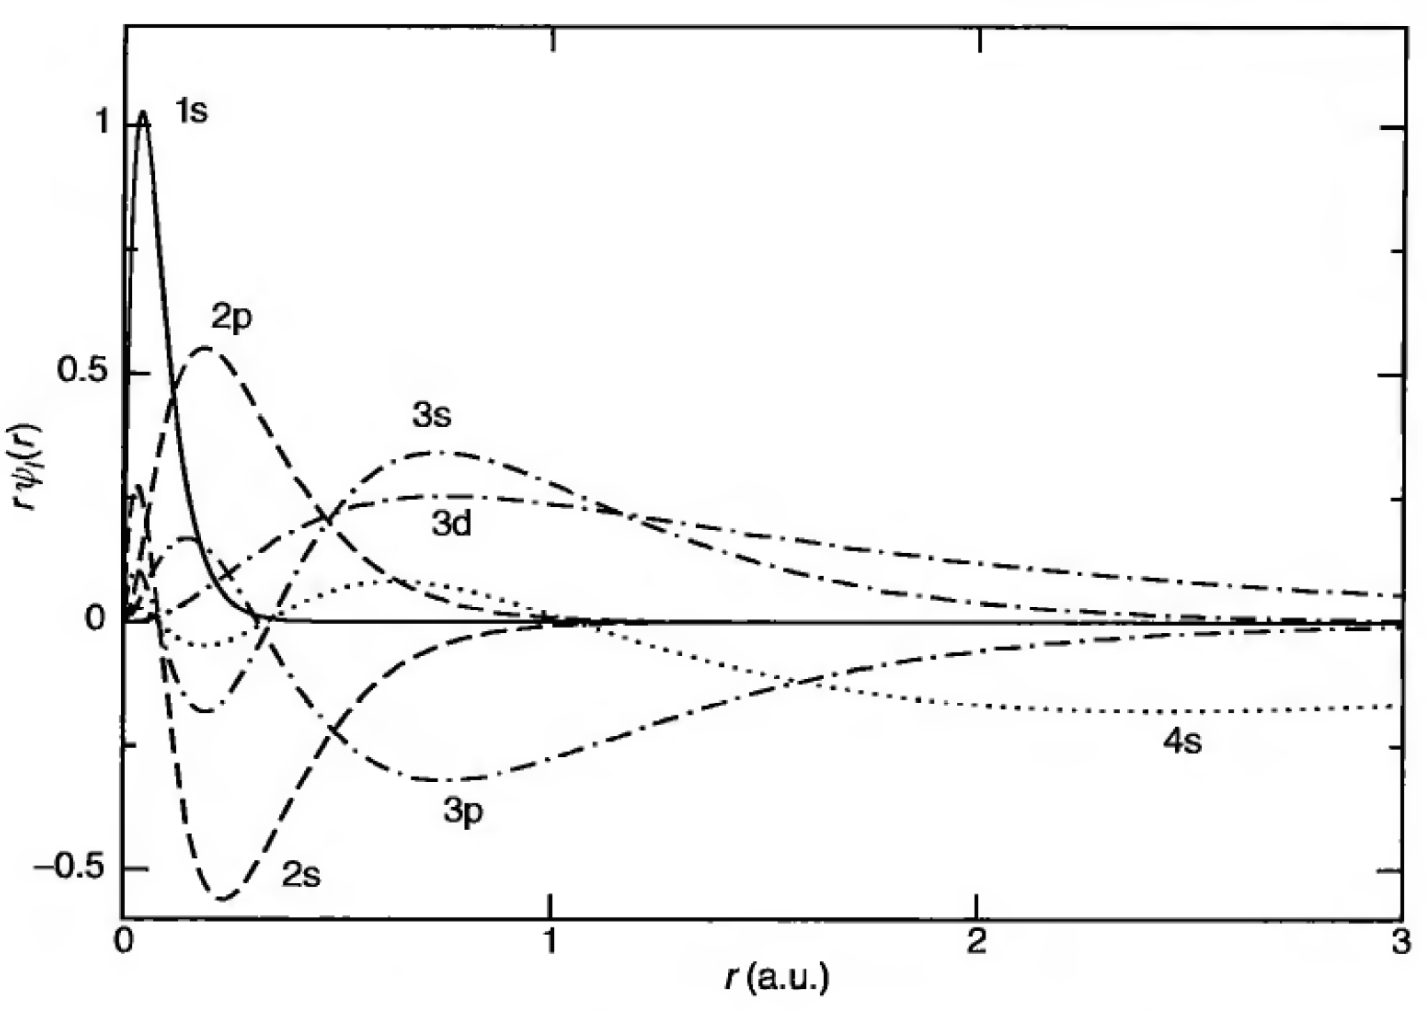
\includegraphics[width=0.9\textwidth]{figures/atomic_radial_wavefunction.png}
    \caption[Radial wavefunction, $r\psi_l(r)$, of Mn in the $3d^{5\uparrow}4s^2$ state showing all atomic orbitals.]{Radial wavefunction, $r\psi_l(r)$, of Mn in the $3d^{5\uparrow}4s^2$ state showing all atomic orbitals. Figure reproduced with permission from Ref.~\citenum{RichardMartin_Ch10}.}
  \label{atomic_radial_wavefunction}
\end{figure}

%** Cross-ref undergrad QM notes? Add eqn for full wavefunction including radial and angular mtm components?? **

The exact, analytical solution of the Schr{\"o}dinger equation for H gives us wavefunctions corresponding to the familiar 1s, 2s, 2p, etc. atomic orbitals. 
In the non-relativistic case (where there is no spin-orbit coupling), the wavefunction can be decoupled as a product of space and spin. Since the nuclear potential acting on the electron is spherically symmetric, the spatial part of the orbital can be described by angular momentum quantum numbers, $L=\{l,m_l\}$ \cite{RichardMartin_Ch10}. This is shown for the hydrogenic one-electron atom in Eq. \ref{SE_rad+ang}, where the full wavefunction is described by the product of the radial and angular distribution functions and expressed in spherical coordinates. The radial component is related to the probability of finding an electron at a particular distance from the nucleus and the angular component is necessary to account for electronic orbitals that are not spherical in shape.
\begin{equation}\label{SE_rad+ang}
\psi_{nlm}(r, \theta, \phi) = R_n(r) Y_{lm}(\theta, \phi)
\end{equation}
Fig.~\ref{atomic_radial_wavefunction} shows the calculated radial wavefunction with all atomic orbitals for a more complicated atomic system, Mn. In this case the system is an open-shell atom and there are unpaired electrons, hence the orbital shapes depend upon the spin. `Spin-unrestricted' calculations require spin functionals and separate $V_{eff}(\mathbf{r})$ for spin up and down. 
%For half-filled shell systems such as Mn, the system is closed-shell when spin up and down are treated separately. For some many-electron systems, the effective independent-particle potential ($V_{eff}(\mathbf{r})$) does not always have spherical symmetry, as it is dependent upon the occupation of the orbitals. In the case of Mn, the potential is spherically symmetric for each closed-shell system when spins are treated separately. However for open-shell systems that are not half-filled a `restricted' approximation can be used to take a spherical average over any non-spherical terms
In a solid, the wavefunctions tend to be atom-like close to each atom. Atomic wavefunctions are closely related to the radial atomic-like functions used in electronic structure codes to represent wavefunctions for solid-state systems \cite{RichardMartin_Ch10}. Accurate description of the electronic structure of atoms is therefore a vital starting point for computing the properties of valence electrons in molecules or solids, which predominantly determine the bonding in the material \cite{RichardMartin_Ch11}. This knowledge is the basis for constructing numeric atom centred orbitals (NAOs) and ab initio pseudopotentials (PPs) as used in the Fritz Haber Institute ab initio molecular simulations (FHI-aims) \cite{FHI-aims} software package and the Vienna Ab-initio Simulation Package (VASP) \cite{VASP} to predict the electronic structure of molecules and solid state systems, which will be outlined next.

Eq.~\ref{basis_set} shows the expansion of the KS orbitals in terms of a set of known functions, called a basis set. 
\begin{equation}\label{basis_set}
\psi(\mathbf{r}) = \sum_j c_j \phi_j(\mathbf{r})
\end{equation}
Constructing a basis set of linearly independent functions allows the use of linear matrix methods and efficient computational tools to solve the KS eigenvalue problem. There are different options for how to mathematically represent the wavefunction. In this work, two different software packages are used for electronic structure calculations, which make use of different functions for their basis sets. 
%These are outlined next along with comments on their relative merits in terms of chemical accuracy and computational efficiency.

%\begin{figure}[h!]
%  \centering
%    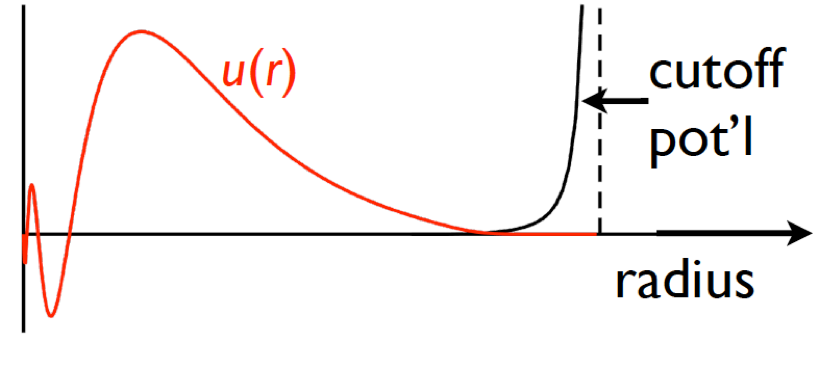
\includegraphics[width=0.6\textwidth]{figures/aims_NACBF.png}
%    \caption{Schematic representation of a numeric atom-centred orbital (NAO) basis function as used in the FHI-aims software package. Taken from Ref. \citenum{FHI-aims_slides}.}
%  \label{aims_NACBF}
%\end{figure}

In the FHI-aims software package, numeric atom-centred orbital (NAO) basis functions, such as that shown in Eq.~\ref{aims_basis_set}, are the basis set used. This basis set for each atomic species has been established from iterative automated construction based on dimers \cite{FHI-aims_slides}. The radial shape, $u_i(r)$, is numerically tabulated and so fully flexible, enabling the creation of optimised element-dependent basis sets that are as compact as possible to minimise computational expense. A schematic represenatation of a NAO is shown in Fig.~\ref{NACBF+PP}a.
\begin{equation}\label{aims_basis_set}
\phi_{NAO}(\mathbf{r}) = \frac{u_i(\mathbf{r})}{r} Y_{lm}(\Omega)
\end{equation}
The NAO basis set used in FHI-aims is localised and highly scalable for use on modern high-performance computing (HPC) systems with multiple processors. The localised nature of the basis set has the benefit of no additional computational cost for vacuum gaps in the simulation unit cell. This implementation of electronic structure calculations is an example of an `all-electron' approach, which has benefitted greatly from advances in HPC technology. 
%However, other highly-successful and computationally efficient approaches for electronic structure calculations of solids have been developed, largely prior to the HPC boom, that are not all-electron but have demonstrated accurate calculated chemical properties.

\begin{figure}[h!]
  \centering
    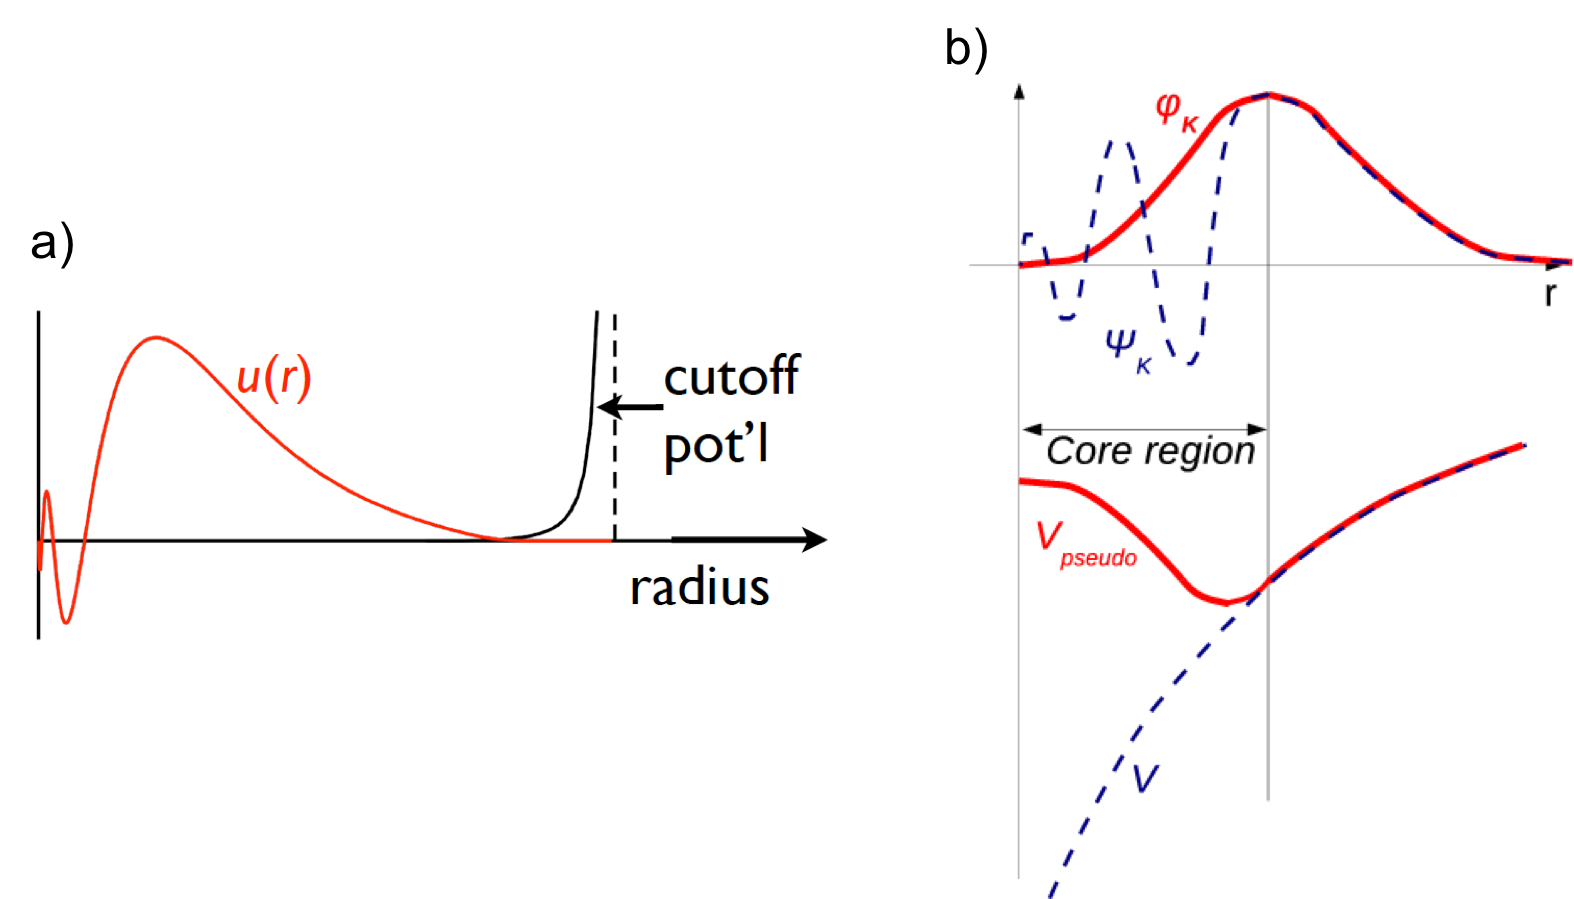
\includegraphics[width=0.95\textwidth]{figures/NACBF+PP.png}
    \caption[a) Schematic representation of a numeric atom-centred orbital (NAO) basis function as used in the FHI-aims software package. b) Schematic representation of a pseudopotential and pseudo-wavefunction (both shown by red solid lines) and corresponding original Coulomb potential and wavefunction (both shown by dashed blue line), where both red and blue lines converge at distances beyond the core region.]{a) Schematic representation of a numeric atom-centred orbital (NAO) basis function as used in the FHI-aims software package. Figure reproduced with permission from Ref.~\citenum{FHI-aims_slides}. b) Schematic representation of a pseudopotential and pseudo-wavefunction (both shown by red solid lines) and corresponding original Coulomb potential and wavefunction (both shown by dashed blue line), where both red and blue lines converge at distances beyond the core region. Figure reproduced with permission from Ref.~\citenum{PP_ref}.}
  \label{NACBF+PP}
\end{figure}

In the VASP software package \cite{VASP} plane waves (PW), as shown in Eq.~\ref{vasp_basis_set}, are used as the basis set. 
\begin{equation}\label{vasp_basis_set}
\phi_{PW}(\mathbf{r}) = ce^{i(\mathbf{k}+\mathbf{G}).\mathbf{r}}
\end{equation}
%In principle, a plane-wave expansion is an infinite expansion and so in practise the expansion must be truncated at some point where a compromise between accuracy and computational efficiency is made. This will be discussed further in section \ref{chem_acc_vs_eff}. 
Plane waves are a natural choice for describing the smoothly varying region of the wavefunction far from the atom cores, i.e. in the interstitial regions. Even a small number of plane waves can accurately represent such a function. However, as can be seen from Fig.~\ref{atomic_radial_wavefunction} and \ref{NACBF+PP}b, the wavefunction oscillates much more rapidly closer to the atom core. This results in much poorer convergence of a plane-wave expansion of the functional. This would require a much larger basis set to accurately describe the system, hence increasing the computational expense \cite{Prasad_ch5}. To improve computational efficiency, without sacrificing chemical accuracy, one technique implemented in the VASP electronic structure code is a formalism of the projector-augmented wave (PAW) method \cite{PAW} that makes use of the pseudopotential and frozen-core approximations \cite{PAW_VASP}, outlined next.

A key concept is to distinguish between `core' and `valence' electrons. Core electrons are tightly bound to the nuclei and their wavefunctions are well localised at lattice sites \cite{Prasad_ch5}. Core electrons usually do not take part in bonding between atoms, therefore it is the valence electrons far from the atom centres that are the most important for determining the bonding in solids. This is the justification for the frozen-core approximation, where core electron states are pre-calculated in an atomic environment and kept unchanged during the course of subsequent calculations for the solid-state system \cite{vasp_slides_PP1}. The strong Coulomb potential of the nucleus and effects of tightly bound core electrons are replaced by an effective ionic potential acting on valence electrons \cite{RichardMartin_Ch11}. The rapid oscillations of the frozen states, however, are used in the orthogonalized plane wave (OPW) method to accelerate the convergence of the expansion used to represent the valence electrons. All solutions of the KS equation corresponding to different energies should be orthogonal to all of the core functions \cite{Prasad_ch5}.

%\begin{figure}[h!]
%  \centering
%    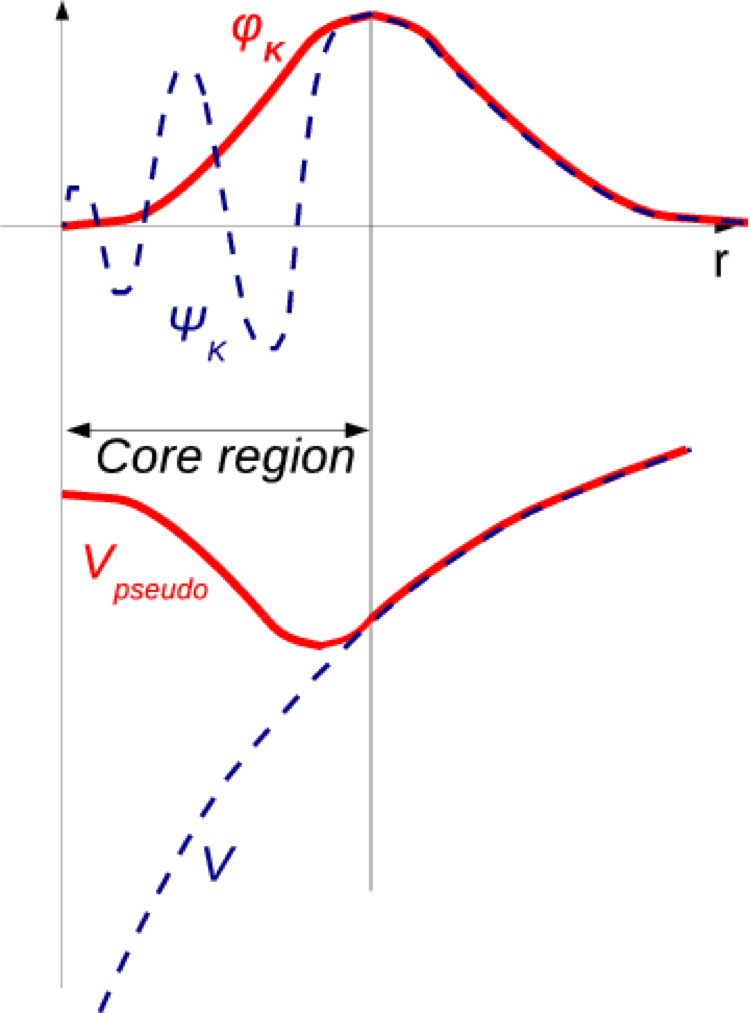
\includegraphics[width=0.45\textwidth]{figures/PP.png}
%    \caption{Schematic representation of a pseudopotential and pseudo-wavefunction (both shown by red solid lines) and corresponding original Coulomb potential and wavefunction (both shown by dashed blue line), where both red and blue lines converge at distances beyond the core region. Taken from Ref. \citenum{PP_ref}.}
%  \label{PP}
%\end{figure}

Furthermore, to accurately describe bonding in solids, it is not necessary to accurately describe the wavefunction at all distances from the nucleus. For a given material there will be some critical radius from the ion cores where physically relevant processes begin to take place, such as inter-atomic wavefunction overlap for bond formation. This is where the pseudopotential approximation is invoked. The true ionic potential is replaced by a much smoother pseudopotential within some critical radius. The aim is that the corresponding pseudo-wavefunction will be smooth and therefore can be represented by fewer plane waves, whilst still reproducing the original wavefunction in the physically relevant regions of space. Fig.~\ref{NACBF+PP}b is a schematic representation of the Coulomb potential, the pseudopotential that is smoothed close to the core region and the corresponding original wavefunction and the pseudo-wavefunction. High-quality pseudopotentials are vital for accurate electronic structure calculations with this method. 

%When the pseudo-wavefunction is expanded in terms of OPWs, a projection operator is used to project the function onto the core states. In contrast to the true wavefunction, the pseudo-wavefunction is smooth and contains only a few plane waves \cite{Prasad_ch5}
The PAW method combines ideas of the linear augmented-plane-wave (LAPW) method \cite{LAPW} with ultrasoft pseudopotential methods \cite{ultrasoft_PP, ultrasoft_PP_VASP, VASP_wiki_PAW}. Ultrasoft PPs reduce the number of plane waves needed by relaxing the norm-conservation requirement for the charge density for the PP. As the norm of the pseudo-wavefunction is not conserved, there is a charge deficit which is compensated by augmentation charges introduced into the core regions \cite{Prasad_ch5}. To combine this with ideas from the LAPW method, the all-electron valence wavefunction, $\psi_{AE}$, is separated into smooth pseudo-wavefunctions, $\psi_{PP}$, and rapidly varying contributions localised within the core region, projectors and auxiliary localised functions respectively. In the PAW approach, integrals are evaluated as a combination of integrals of smooth functions extending throughout space and localised contributions from radial integration over `muffin-tin' spheres \cite{RichardMartin_Ch11}. The $\psi_{AE}$ is related to the $\psi_{PP}$ by a linear transformation. The KS equations are solved to obtain $\psi_{PP}$, which are then transformed back to true wavefunctions (which also incorporate the localised core-region functions) before calculating the charge density and total energy \cite{Prasad_ch5}.
Although the two electronic structure codes described here represent the wavefunction differently when performing electronic structure calculations, a benchmark study comparing results from 15 different solid-state DFT codes to compute the equation of states for 71 elemental crystals showed that all codes converged towards the same result, within error margins comparable to those of experimental measurements \cite{delta_project}. 


%The PAW method is analogous to pseudopotentials in that the primary objects in the calculation are projection operators acting on smooth valence functions \cite{RichardMartin_Ch13}. 

%See: https://cms.mpi.univie.ac.at/wiki/index.php/PAW\_method \cite{VASP_wiki_PAW}
%+ RM pg 225 + 258 \cite{RichardMartin_Ch13}
%+ Prasad pg 144 \cite{Prasad_ch6} + ch7 for LAPW

%RM sections:
%Ch11: pg 204 for summary of pseudopotentials, pg 207 for OPWs, pg 222 for ultrasoft, pg 225 for PAW to allow full wavefunction
%Ch12:  c.f. Bloch theorem and grids
%Ch13: pg 258 for PAW



\subsubsection{Iterative electronic and geometric optimisation}
\begin{figure}[h!]
  \centering
    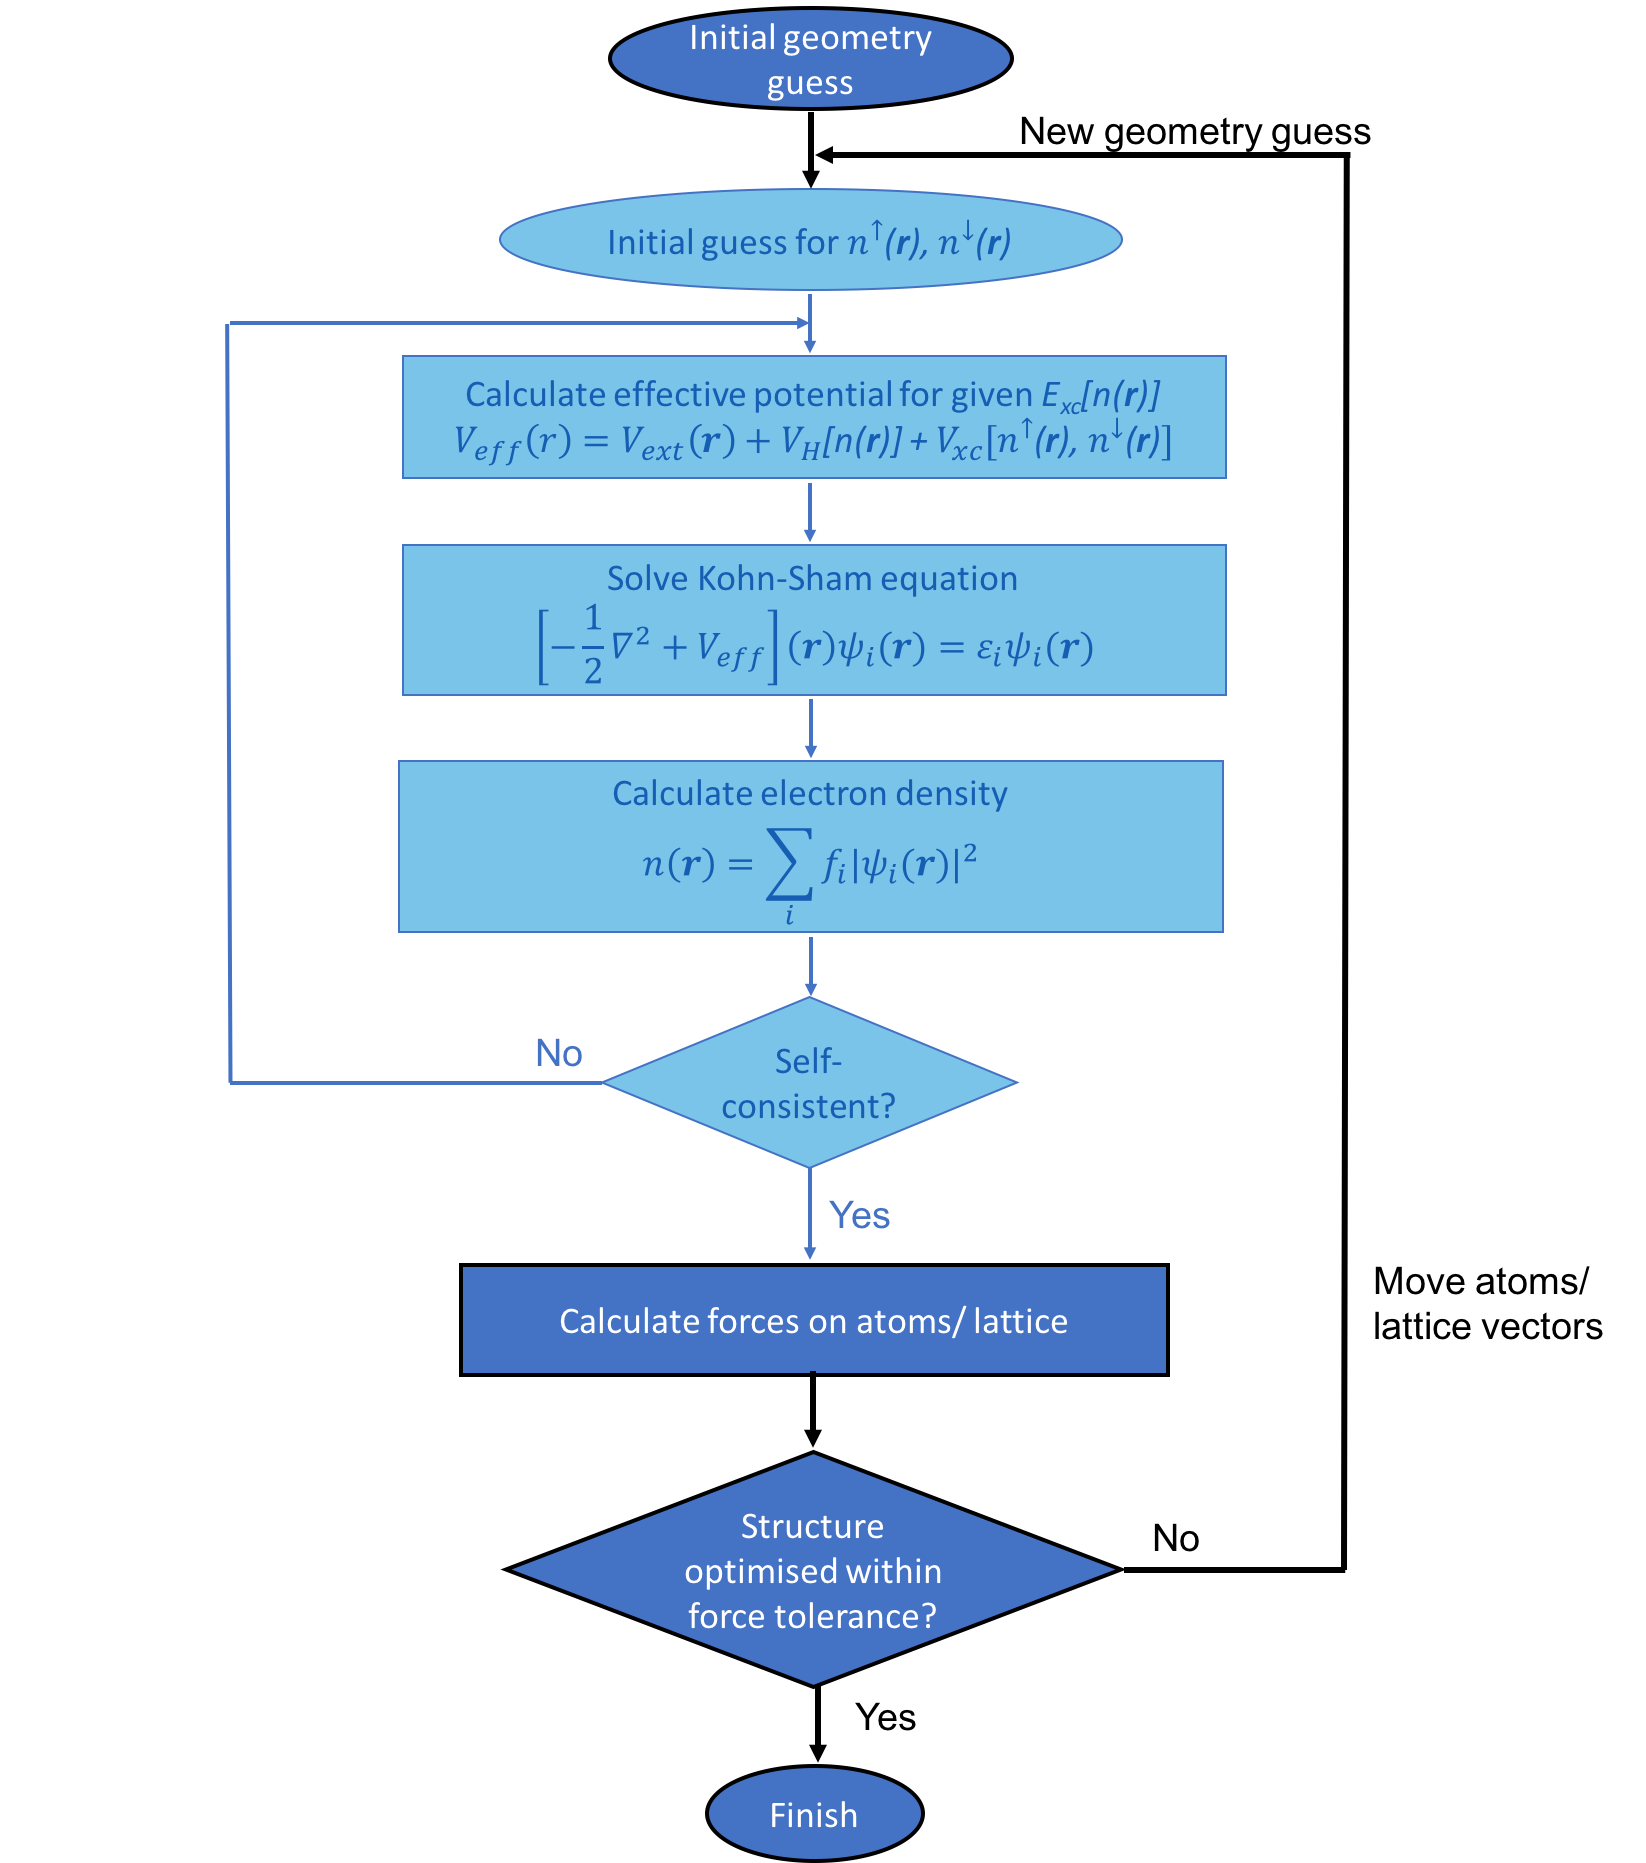
\includegraphics[width=0.95\textwidth]{figures/scf_flowchart.png}
    \caption[Schematic representation of iterative local geometry optimisation procedure with nested self-consistent solution of the Kohn-Sham equations to determine the ground state electron density for each ionic configuration. Darker blue represent iterative steps for geometry optimisation, lighter blue represent SCF electronic convergence.]{Schematic representation of iterative local geometry optimisation procedure with nested self-consistent solution of the Kohn-Sham equations to determine the ground state electron density for each ionic configuration. Darker blue represent iterative steps for geometry optimisation, lighter blue represent SCF electronic convergence. Fig.~adapted from Ref.~\citenum{RichardMartin_Ch9}.}
    \label{SCF_flowchart}
\end{figure}
In this section, the process of optimising the geometry (ionic structure) and electronic structure of a given solid towards the minimum energy configuration (i.e. the ground state) using the self-consistent field (SCF) method for a given electron density functional will be outlined. The SCF method was introduced when discussing the Hartree method for determining $V_H$ and $\psi_i$ that give the minimum total energy for the system within a set tolerance, but it also utilised in the KS formalism of DFT. It is common to use experimental X-ray diffraction data for the atomic arrangement in a solid as a starting point for electronic structure calculations. However, the exact minimum energy arrangement of ions and electrons modelled with a specific exchange-correlation functional will differ slightly. Therefore, an important step in calculating the electronic structure of a material is first to find the minimum energy arrangement of the ions and, in the case of solid-state systems, the lattice parameters for the unit cell that results in the lowest total energy for the given exchange-correlation functional.
\begin{figure}[h!]
  \centering
    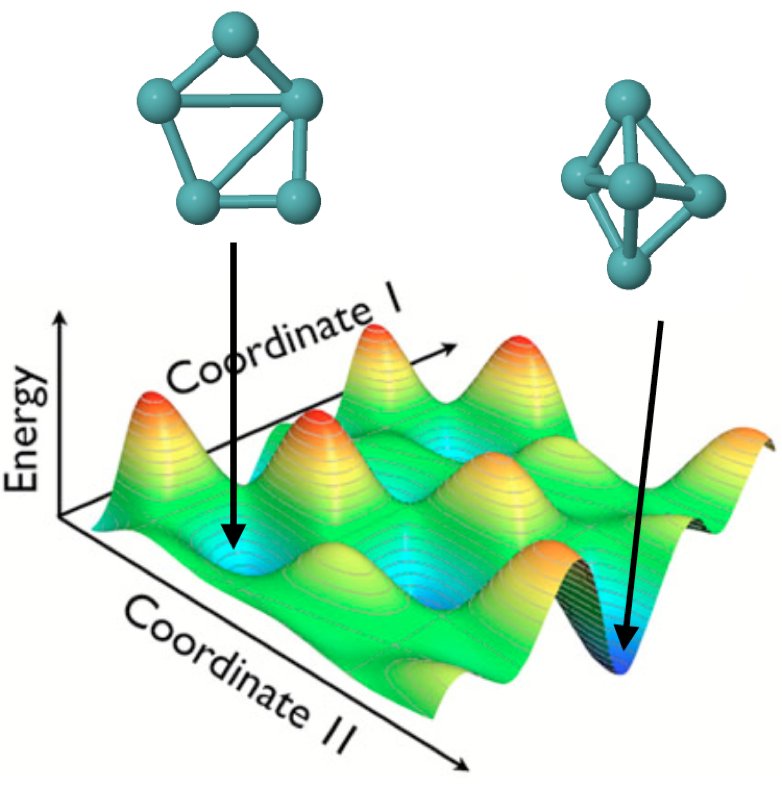
\includegraphics[width=0.4\textwidth]{figures/PE_landscape}
    \caption[Visualisation of minima in the potential energy landscape of a molecular system.]{Visualisation of minima in the potential energy landscape of a molecular system. Figure reproduced with permission from Ref.~\citenum{PE_landscape_ref}.}
  \label{PE_landscape}
\end{figure}

The general procedure for local structure optimisation involves displacing ions in the system (either just ionic coordinates within the unit cell or also including the unit cell dimensions), calculating the electronic structure self-consistently for this static ionic arrangement using the SCF method as indicated in Fig.~\ref{SCF_flowchart}, repeatedly until the forces on the ions are below a given threshold and hence are close enough to their equilibrium, minimum energy positions. The process of geometry optimisation can also be described as searching the potential energy landscape of the system to find the minima, as illustrated in Fig.~\ref{PE_landscape}. Most electronic structure software packages provide options for different optimisation algorithms to converge the system towards a minimum in the potential energy surface. A common approach is to use gradients in the total energy of the system to compute forces on the ions. These methods include the conjugate gradient method and Quasi-Newton appproaches \cite{FHI-aims_slides_Lange}.


\subsubsection{The chemical accuracy and computational efficiency compromise}\label{chem_acc_vs_eff}
Earlier in this section the different mathematical representations of the KS orbitals (i.e. the basis sets) in the electronic structure software packages FHI-aims and VASP were discussed. However, all types of representation are an approximation. It may be necessary to use an infinite set of basis functions to completely represent the KS orbitals. In practice, the basis set must be truncated at some point and then we must check for convergence in the properties of interest with respect to this basis set truncation \cite{Prasad_ch6}. 

\begin{figure}[h!]
  \centering
    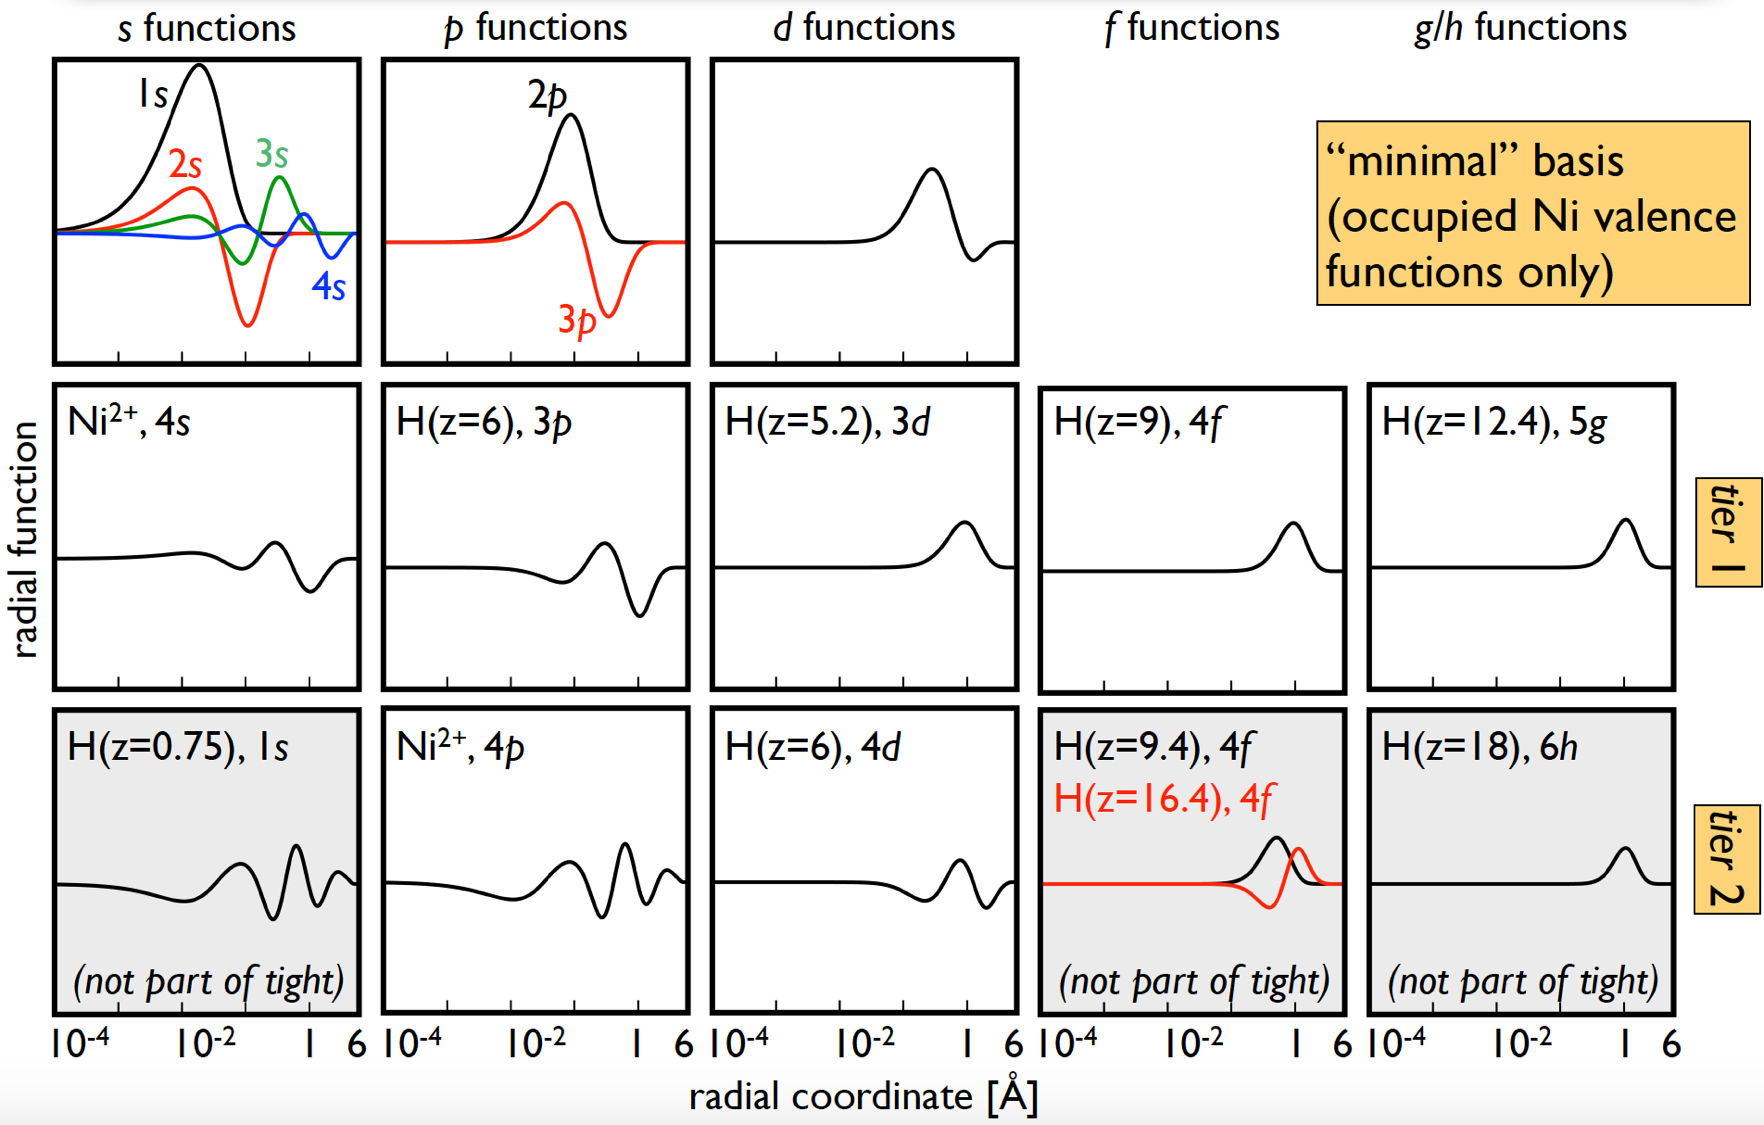
\includegraphics[width=0.95\textwidth]{figures/FHI-aims_tiers.png}
    \caption[Ni radial functions to construct basis sets with increasingly tight convergence criteria as implemented in the software package FHI-aims.]{Ni radial functions to construct basis sets with increasingly tight convergence criteria as implemented in the software package FHI-aims \cite{FHI-aims}. Figure reproduced with permission from Ref.~\citenum{FHI-aims_slides}.}
  \label{FHI-aims_tiers}
\end{figure}

When using FHI-aims, a user can select from a hierarchy of basis (sub)sets that have been organised into `tiers' and tabulated for expected levels of accuracy for each chemical species. The inclusion of additional radial functions (and their angular momenta) for each species are grouped into these tiers, which start from the minimal basis of free-atom like radial functions but users are always recommended to add at least one set of further radial functions that have been optimised to describe a chemical bond with that species.  When using pre-defined calculation settings (`species\_defaults'), additional radial functions are included in the basis set for each species until the required accuracy is reached for settings referred to as `light', `intermediate', `tight' and `really\_tight'. These species\_default settings also define other parameters used in the calculation to achieve the desired level of accuracy, such as the highest order used in the multipole decomposition of the electron density for the calculation of the Hartree potential and the integration grid when the Hamiltonian matrix elements are numerically integrated. The default tight settings are intended to provide meV-level converged energy differences \cite{FHI-aims_manual}. However, users are still encouraged to test the convergence for particular systems. Higher tiers may be required for problematic systems, but it may also be the case that less are required to achieve the desired level of accuracy and hence the computational expense of the calculation could be reduced. Fig.~\ref{FHI-aims_tiers} shows the radial wavefunctions necessary to achieve the `tight' level of convergence for Ni, where `H' in the figure refers to hydrogen-like orbitals. 

The equivalent to the process described above for FHI-aims for electronic structure calculations with VASP is to converge the cutoff energy of the plane wave basis set to achieve the level of convergence desired for the property of interest. In principle, an infinite number of plane waves of increasing frequency (and hence energy) may be necessary in the plane wave expansion. However, in practise this set must be truncated at some point. Similar to the process described above for FHI-aims, the size of the plane wave basis set (determined by the cutoff energy) must be tested to ensure the desired property, often the total energy of the material, is converged to within an acceptable range. Smoother and weaker pseudopotentials require lower cutoff energies \cite{Prasad_ch6}.

\begin{figure}[h!]
  \centering
    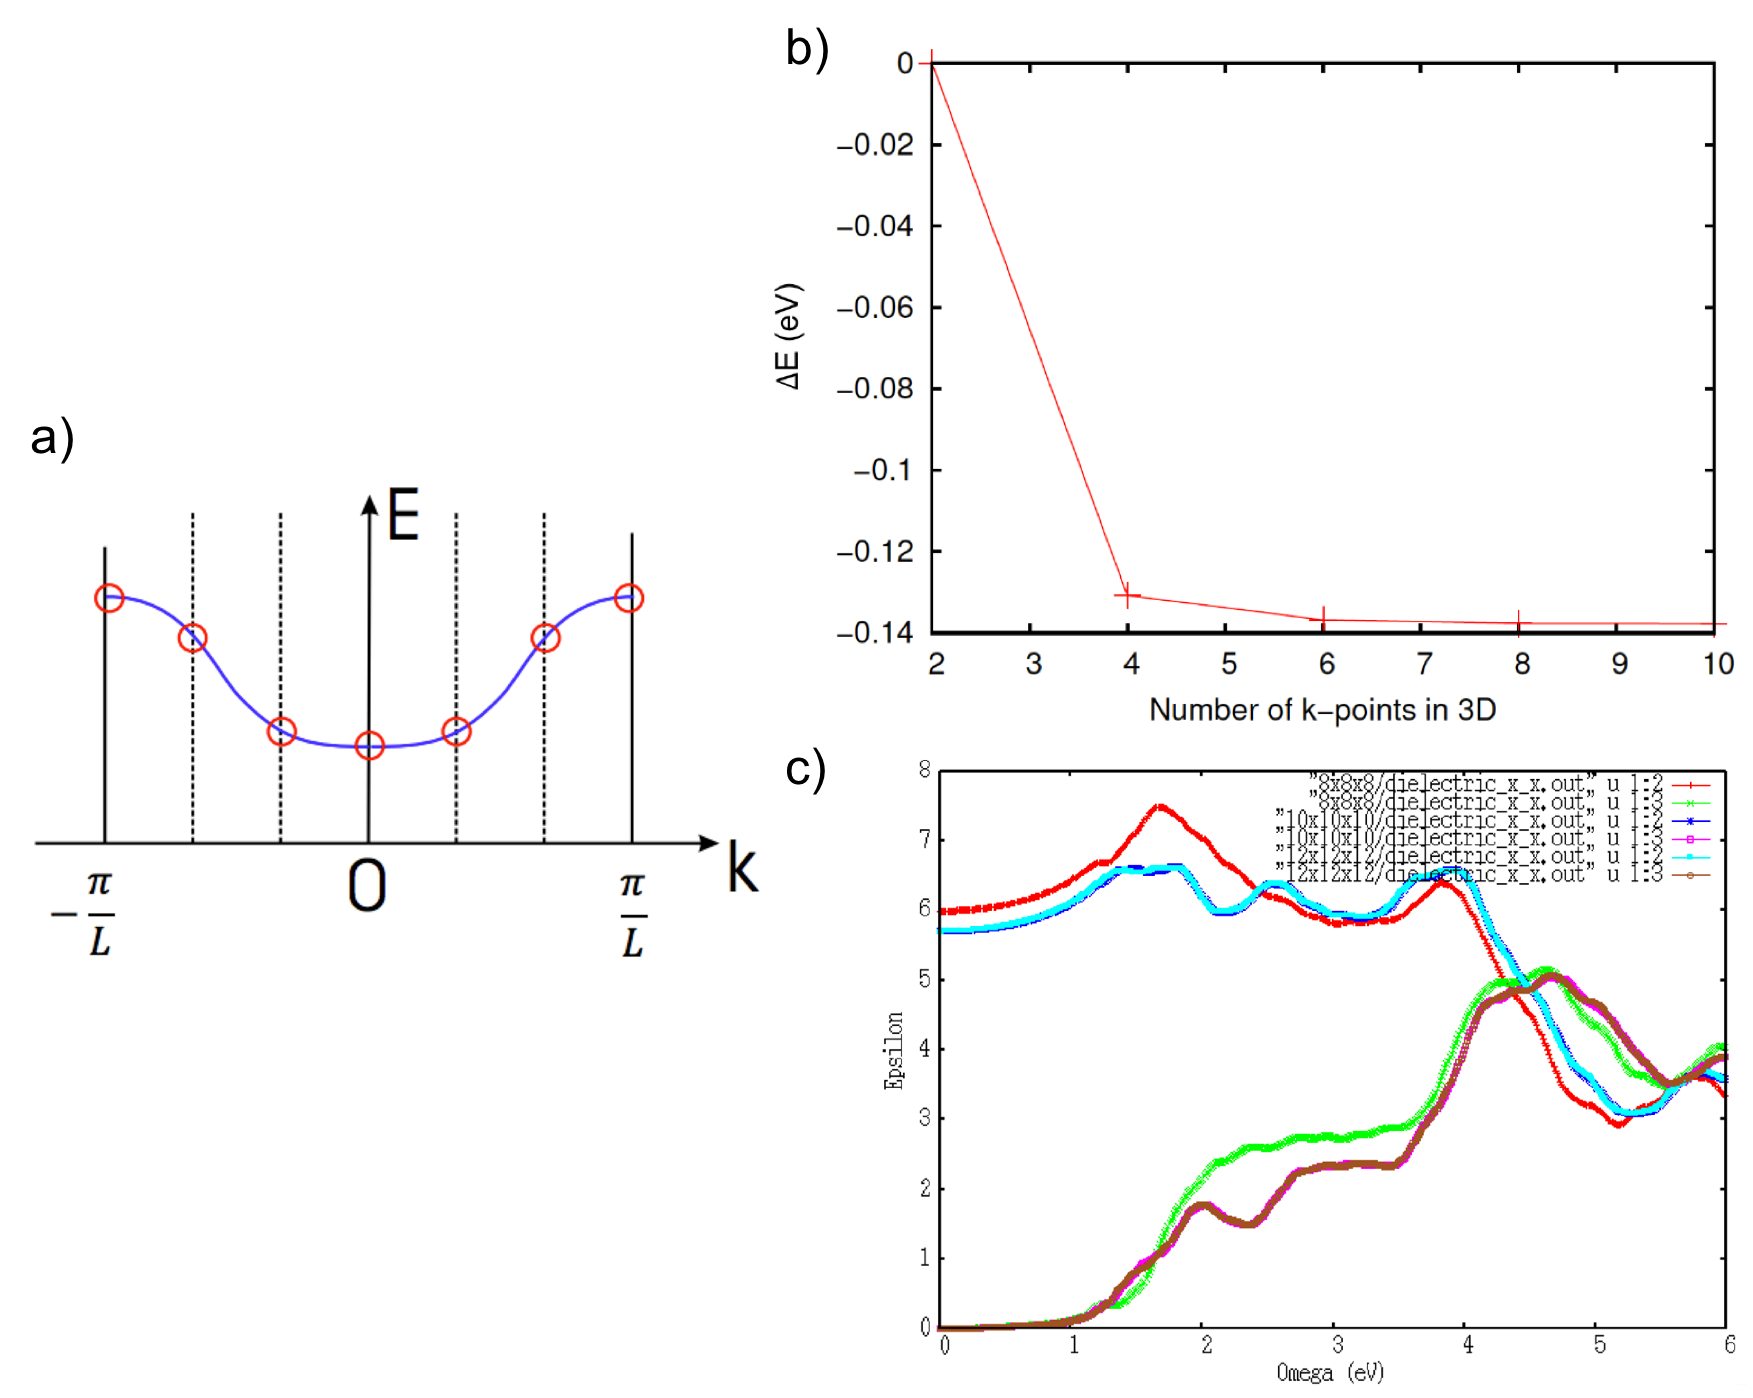
\includegraphics[width=1.0\textwidth]{figures/k-point_sampling_update.png}
    \caption[a) The energy dispersion relation for electrons moving in a crystal, illustrating how the function can be approximately represented by a finite number of \textit{k}-points, forming an equally-spaced mesh. b) convergence of total energy and c) optical dielectric function for the same material.]{a) The energy dispersion relation for electrons moving in a crystal, illustrating how the function can be approximately represented by a finite number of \textit{k}-points, forming an equally-spaced mesh. Figure adapted from Ref.~\citenum{vasp_k-sampling_slides}. Convergence of b) total energy and c) optical dielectric function for the same material.}
  \label{k_sampling}
\end{figure}

For both software packages, the inclusion of a larger basis set increases the computational expense of the calculation, but takes the approximate representations of the KS orbitals closer to the true form and hence improves the accuracy of the calculated material properties for the given electron density functional. Determining the optimal compromise between computational expense and chemical accuracy for the material property of interest is an important process in electronic structure calculations. The other calculation setting that must be considered in such a way is the density of the \textit{k}-grid when sampling the Brillouin zone.

%** Check over below (taken from transfer report) **
% periodic DFT calculations, the total energy is also converged with respect to the number of \textit{k}-points used to sample the Brillouin zone.
As discussed in section \ref{crystal_models}, only the first Brillouin zone of the crystal is needed to fully describe the influence of the periodic lattice on electrons in the solid.
Each electron occupies a state of definite $\mathbf{k}$. In an infinite, periodic crystal structure an infinite number of electrons would result in an infinite number of \textit{k}-points. For many properties of interest, it is necessary to integrate over the Brillouin zone, such as in Eq.~\ref{BZ_int} to obtain the density of electronic states \cite{vasp_k-sampling_slides}.
\begin{equation}\label{BZ_int}
\frac{1}{\Omega_{BZ}} \int_{BZ} F(E)\delta(E_{n\mathbf{k}}-E)d\mathbf{k}    
\end{equation}
Electron wavefunctions will be almost identical for values of $\mathbf{k}$ that are sufficiently close, so the wavefunctions over a region of reciprocal space can be represented by considering the wavefunction at a single \textit{k}-point. Therefore, in practise the integral in Eq.~\ref{BZ_int} is instead evaluated numerically as a weighted sum over special \textit{k}-points, forming a \textit{k}-point mesh or grid \cite{vasp_k-sampling_slides}. A common choice for the \textit{k}-point grid is an equally spaced grid in the Brillouin zone called the Monkhorst-Pack grid \cite{MonkhorstPack}
% Therefore,  At each \textit{k}-point, only a finite number of the available energy levels will be occupied. Therefore only a finite number of electrons need to be considered but at an infinite number of \textit{k}-points. In practise, all of these \textit{k}-points are not considered. 
%It is therefore sufficient to consider the electronic states at a finite number of \textit{k}-points in order to determine the ground state energy of the solid. 
This approximation is illustrated in Fig.~\ref{k_sampling}a. The choice here when setting up an electronic structure calculation is a balance between more \textit{k}-points for a more accurate representation of the Brillouin zone and fewer \textit{k}-points to reduce the computational expense of the calculation. Similar to the process described above for the basis set size, the calculated value of a property of interest should be converged with respect to the \textit{k}-grid density. Certain properties require a denser \textit{k}-grid than others. This is demonstrated in the examples in Fig.~\ref{k_sampling}b and c where the total energy in Fig.~\ref{k_sampling}b required a $6\times6\times6$ \textit{k}-grid to achieve convergence, whereas the optical dielectric function ($\epsilon$) in Fig.~\ref{k_sampling}c of the same material required a $10\times10\times10$ \textit{k}-grid.



\section{First principles prediction of electronic band offsets}\label{band_alignment_methods}
The methodology outlined here is used in the study presented in section \ref{sulfosalt_band_alignment} to screen for candidate junction partners that are predicted to have optimal electronic band offsets for forming a solar cell heterojunction with the absorber layers of interest in the study. The vital function of a solar cell heterojunction (as discussed in section \ref{junctions}) is the separation of photoexcited minority charge-carriers. When selecting a junction partner, therefore, want to know if electrons will easily flow between the conduction bands or holes between the valence bands of the two materials forming the junction. The important material properties to determine this are the electron affinities (EAs) and ionisation potentials (IPs) of the two materials. These are shown schematically in Fig.~\ref{slabs}a. The EA and IP are referenced to the energy of the vacuum level. The EA corresponds to the energy involved in adding an electron to the CB of a material while the IP corresponds the the energy involved in removing an electron from the VB of the material. These quantities are influenced by the bulk binding energy of the material, but as electrons are added to or removed from the surface of a material, are also influenced by the dipole that arises from the redistribution of charges at a surface. It is therefore necessary to also simulate the surface of the material to compute these quantities.

\begin{figure}[h!]
  \centering
    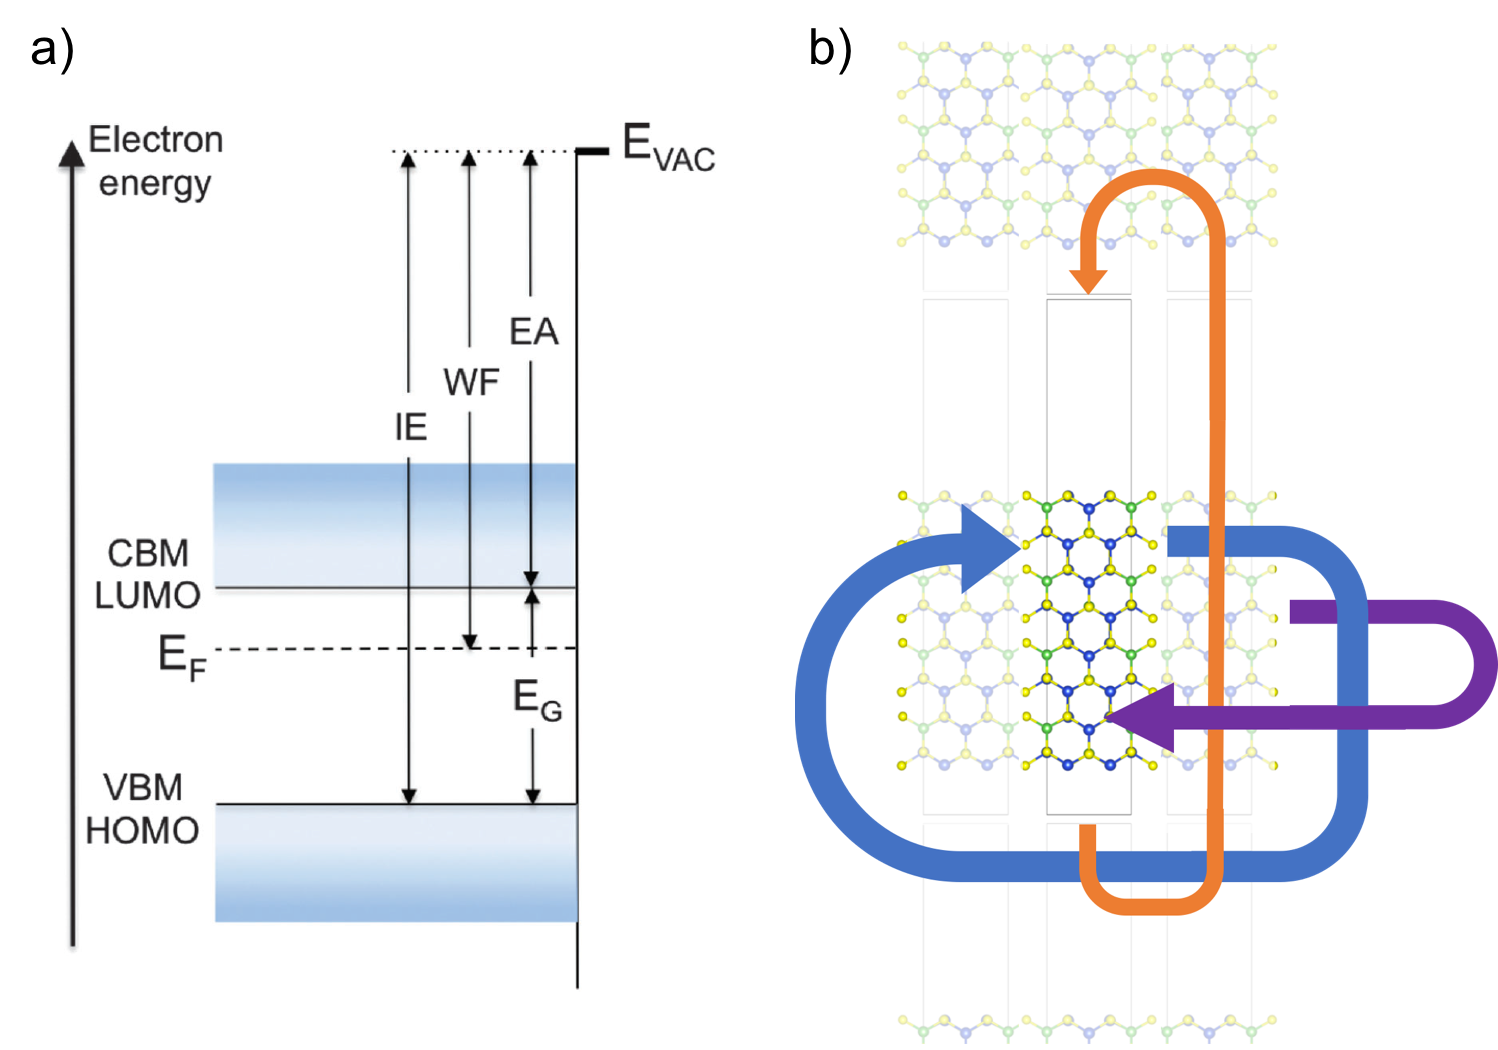
\includegraphics[width=0.9\textwidth]{figures/slab_figs.png}
    \caption[a) Energy diagram of a semiconductor with flat bands to the surface. Indicating the band edges (CBM/LUMO and VBM/HOMO), vacuum level (E$_{VAC}$), work function (WF), band gap E$_G$, ionization energy IE and electron affinity EA. b) Schematic representation of the implementation of 3D periodic boundary conditions for a 2D surface slab where a sufficiently large vacuum gap is required to ensure the surfaces from either end of the slab do not interact (direction indicated by orange arrow).]{a) Energy diagram of a semiconductor with flat bands to the surface. Indicating the band edges (CBM/LUMO and VBM/HOMO), vacuum level (E$_{VAC}$), work function (WF), band gap E$_G$, ionization energy IE and electron affinity EA. Figure reproduced with permission from Ref.~\citenum{electronic_band_edges}. b) Schematic representation of the implementation of 3D periodic boundary conditions for a 2D surface slab where a sufficiently large vacuum gap is required to ensure the surfaces from either end of the slab do not interact (direction indicated by orange arrow).}
  \label{slabs}
\end{figure}

\subsubsection{Surface models}
To simulate a 2D surface with 3D periodic boundary conditions, it is necessary to use a suitably large vacuum gap to ensure that the two surfaces either end of the slab model do not interact with each other \cite{Prasad_ch6}. This is shown schematically in Fig.~\ref{slabs}b.
For a given crystal structure, there are a large number of possible surface terminations when creating the slab model. Where experimental data is available, often this can provide guidance for which terminations are likely to be the most energetically likely to form or to be of the greatest technological interest and therefore inform the design of the slab models. In cases where there is no such experimental data, surface terminations with no net dipole perpendicular to the surface are expected to have the lower surface energies and therefore be more likely to form \cite{Tasker}. The latter informed the choice of surface terminations for the slab models used in section \ref{sulfosalt_band_alignment}.


\subsubsection{Calculation of ionisation potentials}

\begin{figure}[h!]
  \centering
    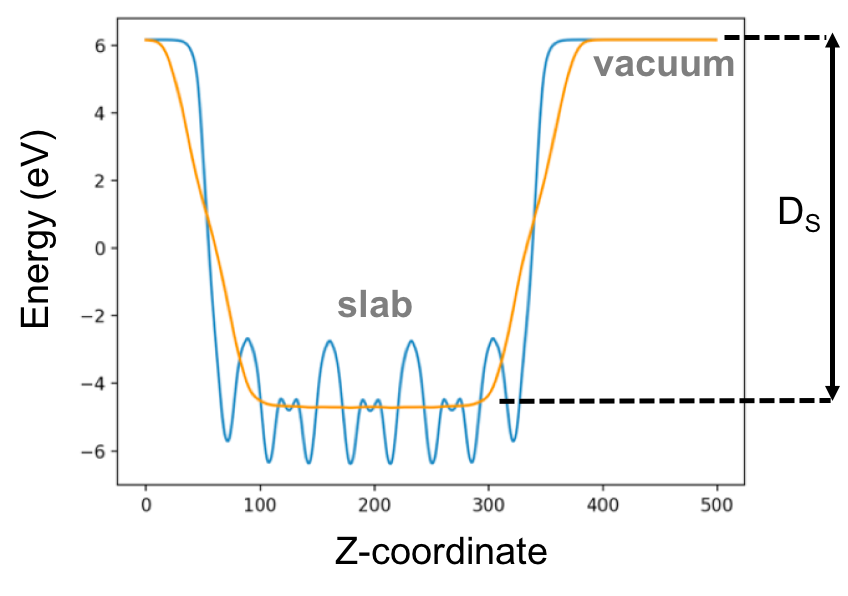
\includegraphics[width=0.6\textwidth]{figures/MD_eg.png}
    \caption[Planar average (blue line) and macroscopic average (orange line) of the potential across the finite direction of a slab model indicating the slab region, vacuum gap and surface dipole, $D_s$.]{Planar average (blue line) and macroscopic average (orange line) of the potential across the finite direction of a slab model indicating the slab region, vacuum gap and surface dipole, $D_s$. Plot generated using the MacroDensity python library \cite{MacroDensity}.}
  \label{MD_eg}
\end{figure}

The alignment of the valence band energy to the vacuum level, i.e. the IP, is a physically well-defined quantity and can be measured using techniques such as photoelectron spectroscopy or Kelvin probe microscopy. The IP can also be quantified using first-principles calculations. In section \ref{sulfosalt_band_alignment}, the macroscopic average technique is used to decompose contributions from the bulk and the surface of the material when calculating the IP \cite{macro_pot_IP}.
Firstly, in the slab models discussed above, if we define the \textit{z}-axis as the finite direction (i.e. normal to the surface), then the geometry of the slab models is periodic in the (x, y) planes. This allows for the simplification of the charge density to a function of the \textit{z}-coordinate only by taking planar averages \cite{band_engineering}, as shown in Eq.~\ref{planar_av} where S is the surface area of planar slices.
\begin{equation}\label{planar_av}
\bar{f}(z) = \frac{1}{S}\int_S f(x,y,z)dxdy
\end{equation}
The macroscopic average is then obtained from Eq.~\ref{macro_av} where a is the unit cell length in the finite direction.
\begin{equation}\label{macro_av}
\bar{\bar{f}}(z) = \frac{1}{a} \int_{z-\frac{a}{2}}^{z+\frac{a}{2}}  \bar{f}(z) dz
\end{equation}

Fig.~\ref{MD_eg} shows the rapid oscillations in the planar average of the potential for each layer in the slab, the plateau far from the slab into the vacuum gap (blue line) and also the smoother macroscopic average of the planar potential (orange line).
The difference between the macroscopic average of the vacuum potential and the bulk-like region of the surface slab is then used to obtain the surface dipole, $D_s$, as shown in Fig.~\ref{MD_eg}.  The eigenvalue of the valence band maximum (VBM) of the bulk, $\epsilon_{VBM}$ and $D_s$ are then used to obtain IP as shown in Eq.~\ref{IP}.
\begin{equation}\label{IP}
IP = D_s - \epsilon_{VBM}
\end{equation}
The other important quantity for determining band offsets at semiconductor-semiconductor junctions is the EA. As shown in Fig.~\ref{slabs}a, this is defined as the conduction band energy with respect to the vacuum level and can be obtained by subtracting the value of the electronic band gap from the IP of the material. 




\subsubsection{Electron affinity rule}
Once the IPs and EAs of the two materials forming the heterojunction have been determined, the electron affinity (or Anderson's) rule can be used to calculate offsets between the conduction bands and valence bands of two semiconductors brought into contact \cite{Anderson_rule, keith_contacts}.
To obtain the band offsets from the electron affinity rule, the vacuum level of the two materials either side of the heterojunction are aligned to the same energy, the difference between the distance between the CBM and the vacuum (EA) of each material is used to predict the CBO, as shown in Eq. \ref{CBO_calc}, where $EA_{abs}$ denotes the electron affinity of the absorber layer and $EA_{jp}$ is that of the wider-gap heterojunction partner. If $E_g$ of each material is also taken into account then the same model can be used to predict the VBO through the difference in the ionisation potentials ($IP = EA + E_g$). 
\begin{equation}\label{CBO_calc}
\Delta E_c = EA_{jp} - EA_{abs}
\end{equation}
\begin{equation}\label{VBO_calc}
\begin{aligned}
\Delta E_v & = E_{g,jp} - E_{g,abs} - \Delta E_c \\
& = (EA_{abs }+ E_{g, abs}) - (EA_{jp} + E_{g,jp}) \\
& = IP_{abs} - IP_{jp}
\end{aligned}
\end{equation}
It is worth noting that this method is an idealised model. The band energies for each junction partner are calculated in the limit of a large vacuum, while the vacuum separation between the two materials is taken to zero when forming the electrical contact. It does not account for possible interface effects, such as intermixing of species at a heterojunction, or consider the effects of finite temperature on band offsets \cite{Bartomeu_T_effects}. However, this method is used in the study in section \ref{sulfosalt_band_alignment} to provide the initial screening process to limit the search space for device optimisation of the absorber layers in that study.


\section{Modelling imperfect solids: Point defects in the dilute limit}\label{defects_methods}
When a solid forms a regular crystal the energies of the bands, i.e. the band structure, can be predicted exactly, as discussed in section \ref{BandTheorySection}, from electronic structure calculations \cite{Nelson3}.
The electronic band structure of a semiconductor provides a rich source of information for how the material may perform as a solar cell absorber layer. However, in reality, absolutely perfect systems do not exist. The energy cost associated with the creation of a defect can often be countered by the increase in the configurational entropy of the system from the addition of the defect \cite{AshcroftMermin_general}.
There are several types of possible defects in solids, some of which were described in section \ref{defects_impact}. 

Defects are usually present in materials in very small concentrations, such that the concentrations are quantified in units of parts per million of host atoms. For this reason, models of defects often aim to simulate the `dilute limit' where defect-defect interactions are negligible. This section outlines approaches developed in the literature for periodic electronic structure calculations of the formation energy of isolated point defects in the dilute limit.
These methods are applied in section \ref{sulfosalt_defects} to provide the first insights into the defect physics (and likely associated impact on PV performance) of some of the candidate photoferroic absorbers identified in \autoref{chap:screening}. 
%These methods are also compared to an aperiodic calculation on a defect embedded in a large cluster in section \ref{defect_benchmark}.
Defect formation energies under specific synthesis conditions can be used to infer the likely concentrations of particular defects, which may have different impacts on PV performance \cite{Aron_defect_tolerance}. 
However, in cases where defect concentrations exceed that which would be considered the dilute limit, alternative modelling approaches are necessary \cite{high_defect_conc_method, defects_beyond_dilute_lim}. In section \ref{MC}, a method is outlined which is used in \autoref{chap:CZTS} to simulate extended antisite defects in a material with large extents of substitutional disorder, beyond what would be considered as the dilute limit. In this case, the methodology is used to investigate high concentrations of Cu/ Zn disorder in {\CZTS}. 

\subsection{The problem of periodicity}
As discussed in section \ref{crystal_models}, models of crystalline solids are built around the translational symmetry of periodic crystal lattices. This property is exploited in electronic structure calculations where, typically, the smallest possible unit cell is used to represent the crystal structure and periodic boundary conditions (PBCs) are used to simulate an infinite, bulk crystal. It is then possible to predict the bulk properties of the material by solving quantum mechanical equations for the electronic structure of just this small unit cell. However, the introduction of a point defect into this simulated system produces a situation such as that shown in 2D for a slice of the system in Fig.~\ref{defect_PBCs}a. With the implementation of 3-dimensional PBCs for a 3D system, this would correspond to an infinite 3D array of highly concentrated point defects. Defect wavefunctions in adjacent unit cells may overlap. However, in real, crystalline systems defects are typically present in parts per million.  To correctly represent isolated point defects, interactions between defect periodic images must be negligible \cite{freysoldt_rev}.

\begin{figure}[h!]
  \centering
    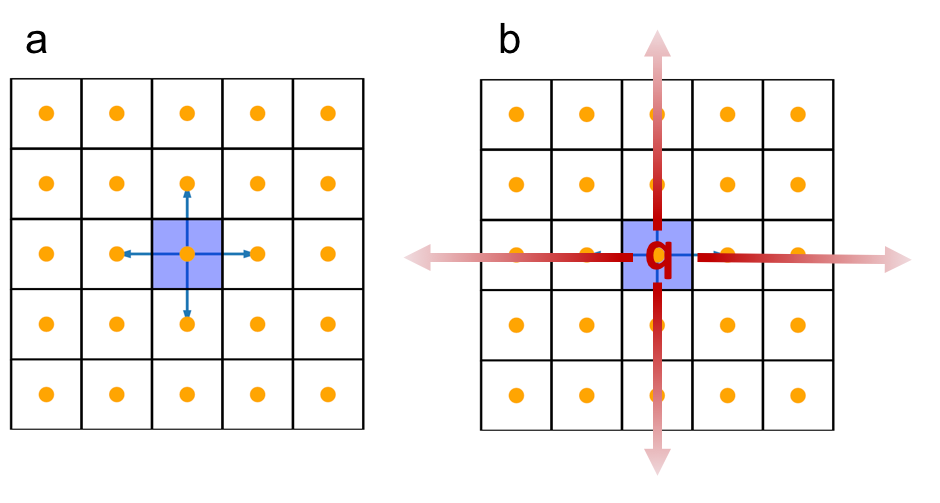
\includegraphics[width=0.75\textwidth]{figures/ase_defects.png}
    \caption[A charge-neutral defect interacting with periodic images of itself across periodic boundary conditions in 2D (a) and the longer-ranged Coulombic interactions of charged defects (b).]{A charge-neutral defect interacting with periodic images of itself across periodic boundary conditions in 2D (a) and the longer-ranged Coulombic interactions of charged defects (b). Figure reproduced with permission from Ref.~\citenum{ase_defects} and adapted.}
  \label{defect_PBCs}
\end{figure}

The supercell method is a common approach to simulate defects in the dilute limit and is the method that is utilised in section \ref{sulfosalt_defects}. This approach involves repeating the primitive unit cell a finite number of times in 3D and then embedding the defect within this larger unit cell so that the defect will be separated from its periodic image by a greater distance. If this distance is sufficiently large, the properties of an isolated defect can be represented by this model \cite{freysoldt_rev}.

\subsubsection{Charge neutral point defects}
The formation energy, $\Delta H_{D,q=0}$, of charge neutral point defects in a supercell can be obtained by comparing the total energy calculated for the defective supercell to that of an equivalent perfect supercell of the host crystal and then considering the species added to or removed from the perfect supercell when the particular defect is formed. $\Delta H_{D,q=0}$ for a charge neutral defect is shown in Eq.~\ref{defect_neutral} where $E_{D,q=0}$ is the total energy of the defective supercell, $E_{host}$ is the total energy of an equivalent supercell of the perfect, bulk host crystal, $n_i$ is the number of atoms of species i added to ($n_i > 0 $) or removed from ($n_i < 0$) the chemical reservoir when the defect is formed. $\mu_i$ is the chemical potential of species i \cite{ZhangNorthup_defect_formation}, referenced to the total energy of the pure element in its standard state, $E_i$. The chemical potential of a species i is the change in energy when one particle of type i is added to the system \cite{chem_pot}. In Eq.~\ref{defect_neutral} $\mu_i$ allows us to describe the formation energy for defects in various growth conditions, such as rich or poor in particular species. If $\mu_i = 0$ then the element is so rich that the pure element phase can form \cite{defects_Chen}.
\begin{equation}\label{defect_neutral}
\Delta H_{D,q=0} = E_{D,q=0} - E_{host} + \sum_i n_i (E_i + \mu_i )
\end{equation}

\subsubsection{Charged point defects}
Additional complexities arise when attempting to obtain the formation energy of a charged isolated point defect. Firstly, there is a strong and long-ranged Coulomb interaction between charged supercells in PBCs (indicated in Fig.~\ref{defect_PBCs}b) and this converges slowly with increased supercell size.
Secondly, the charge of the defect system does not match that of the perfect bulk reference system. It is therefore necessary to introduce a chemical potential to account for the change in energy when electrons are added to or removed from the system when creating a defect in a given charge state.
Thirdly, electronic structure calculations with PBCs for a charged unit cell (effectively) include a neutralising homogeneous background charge to avoid infinite charge, which is not present in the calculation for the perfect equivalent supercell \cite{freysoldt_rev}. Consequently, the expression for the defect formation energy given in Eq.~\ref{defect_neutral} for a charge neutral defect must be modified to that shown in Eq.~\ref{defect_charged}.
\begin{equation}\label{defect_charged}
\Delta H_{D,q} = E_{D,q} - E_{host} + \sum_i n_i (E_i + \mu_i) + q[\epsilon_F + \epsilon_{\nu} + \Delta \nu_{0/b}] + E^q_{corr}
\end{equation}
Additional terms in Eq.~\ref{defect_charged} compared to Eq.~\ref{defect_neutral} are: q (the charge state of the defect), $\epsilon_F$ (position of the Fermi level in the band gap),  $q \epsilon_{\nu}$ (energy of bulk VBM) and $\Delta \nu_{0/b}$ (term used to align the electrostatic potential of the VBM for the bulk and defect supercells) and $E^q_{corr}$ (usually represents multiple post-DFT calculation corrections, one such correction is that for interactions between a charged defect and its periodic images, the `image-charge' correction but another is the `band filling' correction, both of which are outlined later). 
%The latter term is to account for the introduction of the homogeneous background charge in electronic structure calculations of charged supercells, which is discussed further in the next section. 
The terms in Eq.~\ref{defect_charged} are explained pictorially in Fig.~\ref{pylada_eq}.
\begin{figure}[h!]
  \centering
    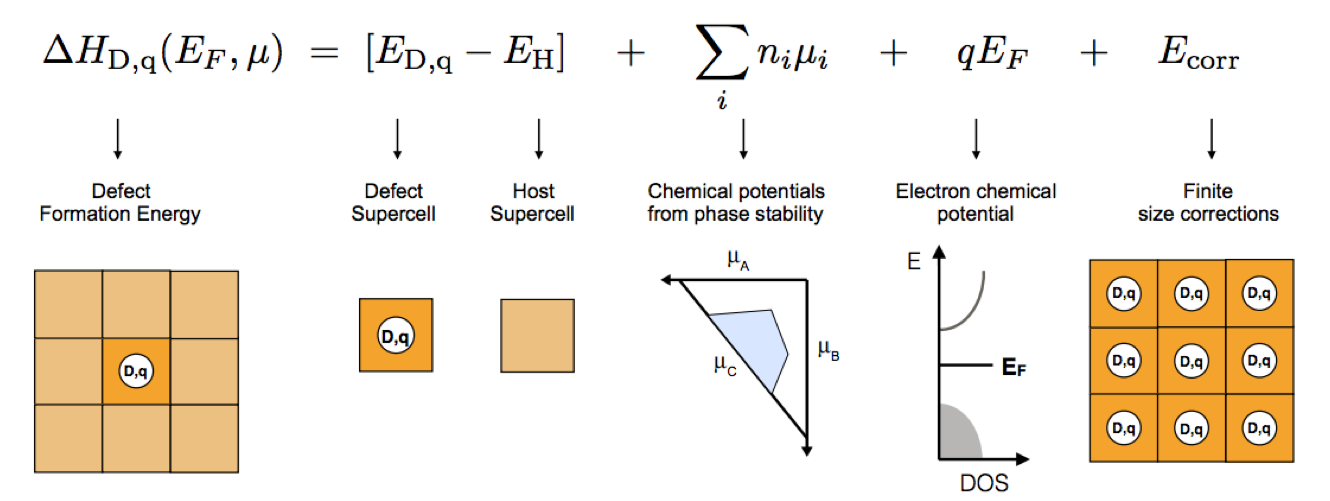
\includegraphics[width=0.95\textwidth]{figures/pylada_eq.png}
    \caption[Visual descriptions of terms in the equation for the formation energy of charged defects.]{Visual descriptions of terms in the equation for the formation energy of charged defects. Figure reproduced with permission from Ref.~\citenum{pylada}.}
  \label{pylada_eq}
\end{figure}

In theory, it is possible to continually increase the supercell dimensions to allow estimations of the magnitude and decay behavior of the different effects to be obtained and, from this, extrapolate to the formation energy of a defect in the limit of an infinitely large supercell. A scaling rule for the correction to the defect formation energy for a supercell with a cubic shape was identified by Castleton et al \cite{supercell_scaling} and is of the form shown in Eq.~\ref{defect_scaling_rule}, where L is the length of the side of the cubic supercell.
\begin{equation}\label{defect_scaling_rule}
\Delta H_{D,q}(L) = \Delta H_{D,q}(L \rightarrow \infty) + \frac{a_1}{L} + \frac{a_3}{L^3}
\end{equation}

Due to computational limitations, it is usually not feasible to perform calculations with sufficiently large supercells to remove all spurious defect-defect interactions, especially for the long-ranged Coulombic interaction of charged defects, as depicted in Fig.~\ref{defect_PBCs}b.
Furthermore, the band gap error in standard-DFT can cause large errors in the calculated properties of defects \cite{Lany_defects, hybrids_defect_calcs}. For this reason, methods beyond standard-DFT such as hybrid-DFT (outlined in section \ref{elec_struc}) may be used to more accurately predict the electronic structure. However, the computational expense for such methods is increased further, hence performing calculations for larger supercells becomes a less feasible endeavor.
Methods such as the supercell approach are used to minimise the impact of defect-defect interactions on calculated properties and various finite-size correction schemes have been developed to correct a posteriori for any remaining effects whenever possible \cite{freysoldt_rev}. These correction schemes have been compared to the extrapolation scheme described above to compare their relative effectiveness for various types of defects \cite{komsa}, although uncertainties in the extrapolation method could be comparable to the errors between different correction schemes \cite{Durrant_defects}. Some of the existing finite-size correction schemes are outlined in the next section. 
%and a study conducted to compare defect formation energies obtained from different finite-size correction schemes for defect supercells to a defect embedded in a large, aperiodic cluster is presented in section \ref{defect_benchmark}.

\subsection{Finite-size corrections to defect supercells}

\subsubsection{Potential alignment}
The formation energy of a charged defect depends on the Fermi level, as shown in Eq.~\ref{defect_charged} and this is referenced to the VBM of the host as the defect formation energy is related to the energy required to add or remove electrons to or from the VBM of the host from or to a Fermi reservoir \cite{Alex_defects}.
However, there are a number of differences between the perfect, bulk system and the charged defect supercell which will cause the average of the potential (even at distances far from the defect) to differ between the perfect and defect supercell, as shown in Fig.~\ref{pa}.
\begin{figure}[h!]
  \centering
    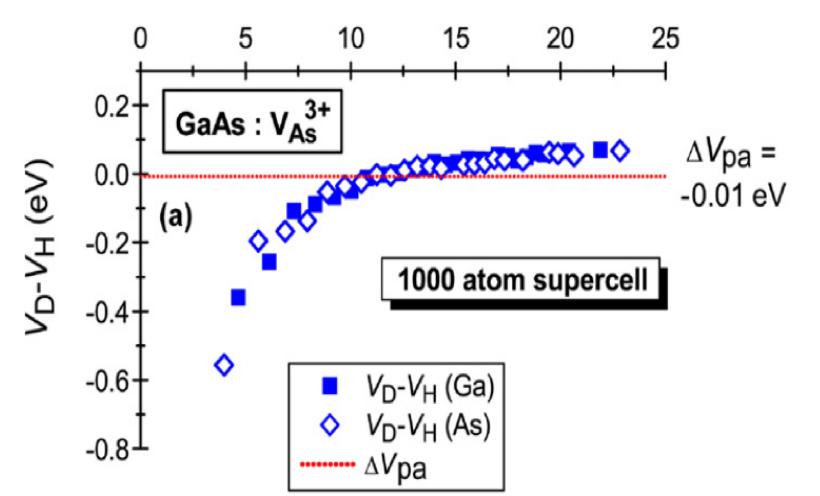
\includegraphics[width=0.7\textwidth]{figures/pa.png}
    \caption[The difference in the atom-site potentials $V_{Ga}$ and $V_{As}$ between a supercell containing a vacancy $V_{As}^{3+}$ and the defect-free host.]{The difference in the atom-site potentials $V_{Ga}$ and $V_{As}$ between a supercell containing a vacancy $V_{As}^{3+}$ and the defect-free host. Figure reproduced with permission from Ref.~\citenum{Lany_defects}.}
  \label{pa}
\end{figure}

Firstly, as the formation of a defect involves addition or removal of ions, this will cause a change in the potential of the system when forming a defect. Secondly, ionic relaxations during defect formation will also perturb the electrostatic potential in the system. Lastly, as already mentioned, when a charged defect is embedded in a supercell in a periodic electronic structure calculation, there will also be a compensating background charge. Otherwise, the Ewald summation performed in the electronic structure code to calculate the electrostatic energy of the system diverges, i.e. the system has an infinite charge. The effect of including a compensating homogeneous background charge is equivalent to setting the average electrostatic potential to zero \cite{freysoldt_rev}. 
In practise this corresponds to removing a constant in the Fourier transform of the electrostatic potential and the consequence of this treatment is that the eigenvalues are defined only up to an undetermined constant \cite{kumagai_oba, kumagai_oba_9}.

This correction step of course will only be applied to the charged defect supercell in the electronic structure calculations, and not to the perfect host. To make matters worse, spurious defect-image charge (which will be discussed in the next section) may also interact with this `homogeneous background charge'.
It is therefore necessary to align the average electrostatic potential in the perfect host supercell to that of the charged defect supercell before computing the defect formation energy through comparisons of the two systems with Eq.~\ref{defect_charged}.
 
Different approaches for potential alignment have been proposed in the literature, including using averages over the electrostatic potential in a small sphere around an atom, as in the Lany-Zunger (LZ) scheme \cite{Lany_defects}, and through the average over transversal planes in the `alignment-like' term in the Freysoldt, Neugebauer, Van de Walle (FNV) scheme \cite{FNV, kumagai_oba}. In both cases, the treatment involves comparing the averaged potential in the bulk-like region of the defect supercell (i.e far from the defect site) to that of a perfect bulk system. Although the electronic structure far from the defect may be similar in the defect supercell and the perfect reference, the average electrostatic potential in equivalent regions of each system could differ by a constant, due to the treatment described above \cite{komsa}. 
%This constant can then be used in Eq. \ref{defect_charged} to align the VBM of the the perfect reference to the defect system.
However, there is some debate in the literature as to whether this potential alignment step is required as a separate correction step, or, if it is in fact accounted for in the image-charge correction (IIC) \cite{kumagai_oba}, which is discussed next for various correction schemes. 


\subsubsection{Image-charge correction}
Image-charge corrections (IICs) are applied a posteriori to calculated total energies of charged defect supercells to account for the spurious interactions of defects with their periodic images, which were depicted in Fig.~\ref{defect_PBCs}, and also with the neutralising `homogeneous background charge'. Most IIC methods involve creating a separate, classical model for these unwanted electrostatic interactions and then subtracting the energy of this interaction from the DFT calculation.

\begin{figure}[h!]
  \centering
    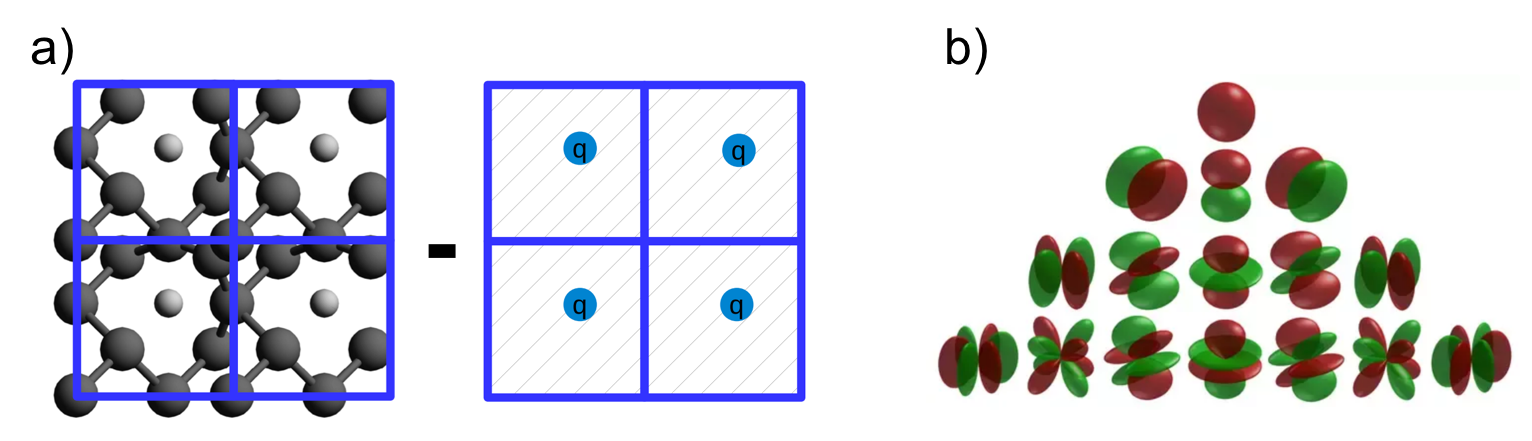
\includegraphics[width=0.8\textwidth]{figures/IIC.png}
    \caption[a) Schematic of first-order Markov-Payne (MP) correction of electrostatic interactions in a periodic DFT calculation of a charged defect where the defect is modelled as a point charge.  b) Multipole expansion of a charge density.]{a) Schematic of first-order Markov-Payne (MP) correction of electrostatic interactions in a periodic DFT calculation of a charged defect where the defect is modelled as a point charge. Adapted from Ref.~\citenum{Durrant_defects}. b) Multipole expansion of a charge density. Figure reproduced with permission from Ref.~\citenum{multipole_web}.}
  \label{IIC}
\end{figure}

The simplest electrostatic model that can be used to quantify the spurious electrostatic interactions in a periodic calculation of a charged defect in a supercell involves approximating the defect as a point charge. The point charge and its periodic images are then considered to interact with each other through a classical dielectric background that represents the host crystal. This is shown schematically in Fig.~\ref{IIC}a where the left figure is the DFT calculation of the defect and the right figure is the model system used to determine the spurious interaction energy to substract from the DFT calculation. The magnitude of interactions between the charged defect with its periodic images can be estimated from the screened Madelung-like energy of an array of point charges. This approach was first used by Leslie and Gillan (LG) \cite{LeslieGillan}. 
\begin{equation}\label{MP}
E^{MP}_{corr} = E_{MP1} + E_{MP2} + ... = \frac{q^2\alpha}{2 \epsilon_s L} - \frac{2 \pi q Q}{3 \epsilon_s L^3} + O(L^{-5})
\end{equation}
The $E_{MP1}$ in Eq.~\ref{MP} is equivalent to the corrections applied by LG where $\epsilon$ is the static (low frequency) dielectric constant of the host crystal and $\alpha$ is the Madelung constant which is only dependant upon the shape of the host supercell. The is the first-order Markov-Payne (MP) correction for cubic supercells.
MP derived a less approximate form for the defect-induced charge density that is still localised, but allowed to be more extended than a point charge \cite{MP}. Later terms in Eq.~\ref{MP} are due to a multipole expansion of the charge density for higher-order terms. An example of a multipole expansion of a charge density is shown in Fig.~\ref{IIC}b. Eq. \ref{MP} only shows odd powers of L as the even powers of L are zero for charge distributions with cubic symmetry \cite{Durrant_defects}.

However, Q in Eq.~\ref{MP} cannot be calculated directly for defects in crystalline materials \cite{Lany_defects_2008}. Therefore in practise when using the MP scheme $E^{MP}_{corr}$ is usually not calculated but is estimated by fitting Eq.~\ref{MP} to the formation energies calculated for defects with increased supercell size and then extrapolating to the infinite supercell limit. As already discussed, at high levels of theory such large systems may be computationally unfeasible. Furthermore, it has been shown that Eq.~\ref{MP} does not always give a good fit to calculated defect formation energies, creating doubt regarding the predictive power of this scheme \cite{FNV}. A number of alternative schemes have been proposed that do not require the use of increasing supercell sizes \cite{MP, LeslieGillan, PeterSchultz, Lany_defects, FNV, kumagai_oba}. Next some such schemes will be outlined. 
%the LZ \cite{Lany_defects} and FNV \cite{FNV} schemes will be outlined as these methods will be used to calculate defect formation energies and the results will be compared in section \ref{defect_benchmark}.

%\begin{figure}[h!]
  %\centering
 %   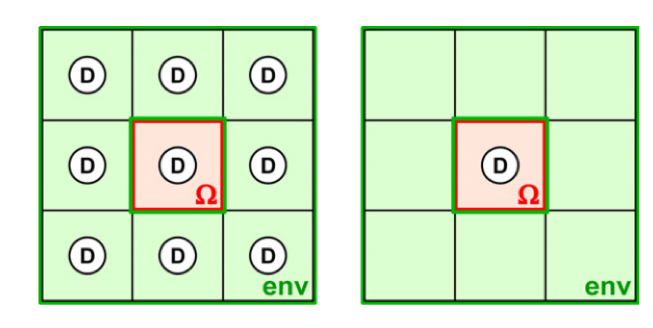
\includegraphics[width=0.8\textwidth]{figures/LZ_ic.png}
%    \caption{A defect supercell of volume $\Omega$ in an environment (env) of periodic images of the defect (left) and in an environment of surrounding perfect, unperturbed supercells of the host lattice (right). Figure taken from Ref. %\citenum{Lany_defects}.}
%  \label{LZ_ic}
%\end{figure}

The MP scheme \cite{MP} discussed above was developed for molecular systems and when calculating Q in Eq.~\ref{MP} the part of the defect charge density due to the electronic screening from the host crystal is not included \cite{Lany_defects_2008, Lany_defects}. However, it has been shown that Q is dominated by this contribution in crystalline solids \cite{Lany_defects_2008}. The LZ scheme, as outlined in Ref.~\citenum{Lany_defects}, was devised to resolve this situation when calculating the IIC for charged defects in crystalline solids.
This method involves a practical approximation to Q that has been determined for supercells with cubic geometry and an isotropic dielectric response \cite{Durrant_defects}.

The LZ method firstly involves the assumption that bound charge is drawn uniformly from the host supercell. For this reason, the method depends on the material having an isotropic response. The polarisation of the bound charge is used to define Q. The LZ scheme effectively involves scaling the MP1 term as shown in Eq. \ref{LZ_Ecorr} where $c_{sh}$ is the shape factor, which only depends on the shape of the supercell. The relation between the LZ and MP schemes (with only odd powers of L) suggests that the LZ methods also makes the assumption of a cubic supercell with zero charge density for even powers of L \cite{Durrant_defects}. In the LZ scheme the potential alignment correction is performed independently of the image-charge correction.
\begin{equation}\label{LZ_Ecorr}
E_{IIC}^{LZ} = [1 + c_{sh} (1 - \epsilon_s^{-1}) ] E_{MP1}
\end{equation}
The FNV scheme, as outlined in Ref.~\citenum{FNV}, differs from the LZ scheme in that it does not depend upon the shape of the supercell and does not involve a separate potential alignment step. In this approach, the defect-induced charge density is modelled as a Gaussian distribution. The electrostatic potential of the model system and the DFT calculation are aligned at regions far from the defect to account for extra polarisation effects when calculating the IIC.

A scheme proposed recently by Durrant et al \cite{Durrant_defects} is quite closely related to the LZ scheme, but makes use of DFT charge density differences and therefore avoids the need of an approximate form for the defect-induced charge distribution. This scheme therefore does not depend on a supercell having cubic geometry or that the dielectric response of the host material is isotropic. The work also systematically decomposes the contributions to the potential alignment to decouple contributions to the potential alignment from those in the image-interaction correction. The study showed that the potential alignment correction was only partly account for by their IIC.


\subsubsection{Band filling correction}

The above correction methodologies require that the charge of the defect is localised within the supercell unit. However, this is not always the case. Large finite-size effects that converge slowly with increased supercell size have been observed for some defects, even in charge neutral states. This has been attributed to ‘band filling’ effects from high defect concentrations in typical finite-size supercells \cite{Lany_defects_2008, CIS_defects, pylada}. This effect is typically more pronounced for shallower defects. Shallower defects typically have more delocalised wavefunctions associated with them, therefore increasing the likelihood of the defect wavefunction extending beyond the boundary of the supercell unit. Consequently, it is possible for even neutral defects to interact with defect-images in adjacent supercells. 

Defect-defect interaction means that the defect-induced energy level may interact with that of its image to form a defect band with a dispersion in the band energies that would not be present for a distinct, localised defect level that would be expected for a defect in the dilute limit. In the case of a donor defect, the electrons may now occupy defect-induced energy levels in the defect band at higher energies than would be possible in the dilute limit due to the dispersion of the defect band. This could then also lead to spurious hybridisation of defect bands with the host electron states, and the donor electrons can partly populate the host conduction bands, giving rise to band filling effects (Moss-Burstein shift) \cite{Lany_defects_2008}.

A correction step for such effects has been proposed \cite{CIS_defects, Lany_defects_2008, Lany_defects} and is to be applied after performing the potential alignment step in the LZ scheme outlined above.
To correct the total energy of the finite supercell due to the band-filling effects, the higher energy populations are subtracted \cite{CIS_defects}.
For a given \textit{k}-point set (weighted sum, $w_k$) and band occupations, $\eta_{n,k}$, the correction for a shallow donor is obtained from Eq.~\ref{band_filling_donor} and for a shallow acceptor from Eq.~\ref{band_filling_acceptor}, where $e_{n,k}$ are the band energies in the defect calculation, $\tilde{e}_c$ and $\tilde{e}_v$ are the CBM and VBM energies respectively of the pure host after performing the potential alignment step within the LZ scheme \cite{pylada}.
\begin{equation}\label{band_filling_donor}
E_{BF} = - \sum_{n,k} w_k \eta_{n,k} [e_{n,k} - \tilde{e}_c]
\end{equation}
\begin{equation}\label{band_filling_acceptor}
E_{BF} = - \sum_{n,k} w_k (1 - \eta_{n,k}) [e_{n,k} - \tilde{e}_v]
\end{equation}
However, if the intention is to simulate defects in highly doped semiconductors, the corrections in Eq.~\ref{band_filling_donor} and \ref{band_filling_acceptor} should be zero or at least smaller since the formation of defect bands with band dispersion and heavy band filling should be present in a system where defect-defect interactions are a correct physical representation \cite{CIS_defects}.


\section{Modelling imperfect solids: Extended antisite defects}\label{MC}
In this section defects and disorder is considered on much larger scales than is computationally feasible from electronic structure calculations.
Here, the fundamentals of utilising the Monte Carlo method to describe thermodynamic substitutional disorder are outlined. This is equivalent to investigating interacting extended antisite defects at higher defect concentrations than would be considered as the `dilute', non-interacting limit. This method is applied to study Cu/ Zn disorder in {\CZTS} in \autoref{chap:CZTS}.
%**Introduce general method (see transfer report + cross-ref extra textbooks** \cite{MC} = Newman, \cite{MC_Landau} and \cite{MC3} (Topic in current physics)

\subsection{The Monte Carlo method for thermodynamic disorder}
The Monte Carlo (MC) method allows for the simulation of systems with many degrees of freedom. Its name derives from its use of (pseudo-)random numbers to simulate statistical fluctuations in order to numerically generate probability distributions \cite{MC3}.
The MC method in statistical physics is a special case of the more general MC method.
Starting from a model hamiltonian, the method can be used to calculate thermodynamic information about a system of N interacting ions represented on a 3D lattice by using classical statistics, considering only two-body forces and assuming that the potential field of an ion is spherically symmetric. If we know the positions of the N interacting ions on the lattice then the potential energy of the system can be calculated using Eq. \ref{pot_E}, where $d_{ij}$ is the minimum distance between ions \textit{i} and \textit{j} with charge $q_i$ and $q_j$  \cite{Metropolis}.
\begin{equation}\label{pot_E}
U = \frac{1}{2} \sum_{i=1}^N q_i \sum_{j=1}^{N(j \neq i)} \frac{1}{4 \pi \epsilon_0}\frac{q_j}{d_{ij}}
\end{equation}

To calculate the properties of the system, the canonical ensemble is used where the temperature, number of ions and volume are all constant. In this ensemble, the equilibrium value for any quantity of interest, B, is given by Eq.~\ref{av}, where $E_\alpha$ is the energy of the system when in state $\alpha$ and $p_\alpha$ is the probability of the system being in state $\alpha$.
\begin{equation}\label{av}
<B> = \frac{ \sum_\alpha e^{-\frac{E_\alpha}{k_bT}} B_\alpha}{ \sum_\alpha e^{-\frac{E_\alpha}{k_bT}}} = \frac{ \sum_\alpha e^{-\frac{E_\alpha}{k_bT}} B_\alpha}{Z} = \sum_\alpha B_\alpha p_\alpha
\end{equation}
\begin{equation}\label{prob}
p_\alpha = \frac{  e^{-\frac{E_\alpha}{k_bT}} }{ \sum_{\alpha} e^{-\frac{E_\alpha}{k_bT}}} =\frac{  e^{-\frac{E_\alpha}{k_bT}} }{Z}
\end{equation}
$Z$ in Eq.~\ref{av} is called the partition function. For most systems calculating the value of the partition function requires the summation over a large number of states. When applying the Monte Carlo method to a system of particles, the summation over discrete states for $Z$ is replaced by a set of integrals. This is shown in Eq.~\ref{MC_av} where $U(\mathbf{r}^N)$ is the potential energy of the system which depends upon the position, \textbf{r}, of the N interacting ions in the system and $Z_{NVT}$ is the configurational integral \cite{Lesar3}.
%\begin{equation}\label{MC_prob}
%p(\mathbf{r}^N) = \frac{  e^{-\frac{U(\mathbf{r}^N)}{k_bT}} }{\int %e^{-\frac{U(\mathbf{r}^N)}{k_bT}} d\mathbf{r}^N}  = \frac{  e^{-\frac{U(\mathbf{r}^N)}%{k_bT}}}{Z_{NVT}} 
%\end{equation}
\begin{equation}\label{MC_av}
<U> = \frac{ \int e^{-\frac{U(\mathbf{r}^N)}{k_bT}} U(\mathbf{r}^N) d\mathbf{r}^N}{\int e^{-\frac{U(\mathbf{r}^N)}{k_bT}} d\mathbf{r}^N}  = \frac{  \int e^{-\frac{U(\mathbf{r}^N)}{k_bT}} U(\mathbf{r}^N) d\mathbf{r}^N}{Z_{NVT}} 
\end{equation}
The configurational integral is over the three coordinates of each ion, as shown in Eq.~\ref{dr}. There are therefore 3N coordinates that define all possible configurations of the system.
\begin{equation}d \mathbf{r}^N = dx_1 dy_1 dz_1 dx_2 dy_2 dz_2... dx_N dy_N dz_N\end{equation}\label{dr}
For a system containing several hundred ions this would be a several-hundred dimensional integral over the configuration space, which would be impractical to carry out by the usual numerical methods. The Monte Carlo method for many-dimensional integrals is used for this purpose \cite{Metropolis}. It is conceptually easiest to think about this method for a one-dimensional integral. This method involves sampling a large number of random points within a region defined by the limits of the integral. The integrated function is then the fraction of points that fall below the curve of the function multiplied by the area of the sampled region. The value obtained becomes a better approximation to the actual value of the integral as the number of random numbers, called Monte Carlo steps (MCS), used to sample the integration region increases. \cite{Lesar3}.


\subsubsection{Monte Carlo simulation with the Metropolis Algorithm }
The Standard MC method for our system would involve placing each of the N ions at random positions in the lattice to define a random point in the 3N-dimensional configuration space. The energy of the system would then be calculated using Eq.~\ref{pot_E} and the configuration would then be weighted using $e^{-\frac{U(\mathbf{r}^N)}{k_bT}}$ when obtaining the equilibrium value of U. However, many configurations are very improbable so performing this calculation for every possible configuration would be inefficient and unnecessary to sufficiently evaluate the ensemble. The custom MC code in this study makes use of the Metropolis modified MC scheme \cite{Metropolis}. In this implementation of the MC method, instead of choosing configurations randomly and then weighting them, the Metropolis algorithm considers the relative probability of a system being in a new configuration, $\beta$, to that of being in the current configuration, $\alpha$. This is shown in Eq.~\ref{relative_prob}, where $E_\alpha$ is the energy of state $\alpha$ and $E_\beta$ is the energy of state $\beta$.
\begin{equation}\label{relative_prob}
\frac{p_\beta}{p_\alpha} = \frac{  e^{-\frac{E_\alpha}{k_bT}} }{Z} \frac{Z}{  e^{-\frac{E_\alpha}{k_bT}} } = e^{- \frac{E_\beta - E_\alpha}{k_BT}}
\end{equation}
The relative probabilities of the two states are completely determined by the energy 
difference, such that if:
\begin{equation}\label{met}
\Delta E = E_{\beta} - E_{\alpha} \leq 0    \quad  then  \quad   \frac{p_{\beta}}{p_{\alpha}} \geq 1 
\end{equation}
and if
\begin{equation}\label{met2}
\Delta E = E_{\beta} - E_{\alpha} > 0   \quad   then   \quad   \frac{p_{\beta}}{p_{\alpha}} < 1
\end{equation}

The Metropolis algorithm creates a list of configurations through configuration space that has the correct probability distribution. This list is called a trajectory through configuration space. The approach involves making a trial move of the system to a new configuration. In the case of the study presented in section \ref{CZTS_MC} \cite{eris_paper} this would be a substitution between a Cu and a Zn ion in an on-lattice model of {\CZTS}. It is then decided if this new configuration should be added to the trajectory or not based on the probability of the new configuration relative to the current configuration. As shown above, the relative probabilities of two states are determined by their energy difference. In the case of the on-lattice model of {\CZTS}, the change in lattice energy before and after a proposed Cu/ Zn substitution is evaluated for every trial MC move. If the relative probability is  $\geq$ 1, as shown in Eq.~\ref{met}, then the move is accepted and added to the trajectory. However, if the relative probability is $<$ 1 then the move will only be accepted if $e^{-\frac{\Delta E}{k_BT}} \ge$ a random number generated between 0 and 1 \cite{Lesar3}. Provided a sufficiently large number of trial moves have been made, from this procedure it is possible to obtain equilibrium disordered configurations for the ions in {\CZTS} at various simulation temperatures. The model developed for {\CZTS} is discussed further in the section \ref{Eris}.






\chapter{Performance bottlenecks of {\CZTS} solar cells}\label{chap:CZTS}
\section{Motivations and challenges for {\CZTS} solar cells}
Thin-film PV technology is a desirable contender for making a major contribution to terawatt-scale renewable energy generation. Kesterite-structured {\CZTS} (CZTS) stands out for its potential for large-scale deployment due to the abundance and non-toxicity of its elemental components, as well as sunlight-matched direct band gap of 1.5 eV \cite{CZTS_rev}. In the following letter we outline the motivations for utilising kesterites as the absorber layer in a solar cell and compare the volume of research efforts directed towards this type of solar cell technology to that for hybrid halide perovskite solar cells. We then go on to discuss some of the most likely bottlenecks preventing the advancement of kesterite-based solar cells.

\subsection{Publication: The steady rise of kesterite solar cells}
%\subsection{**Statement of authorship}


\includepdf[pages={1-},scale=1.0]{papers/CZTS_letter_soa.pdf}

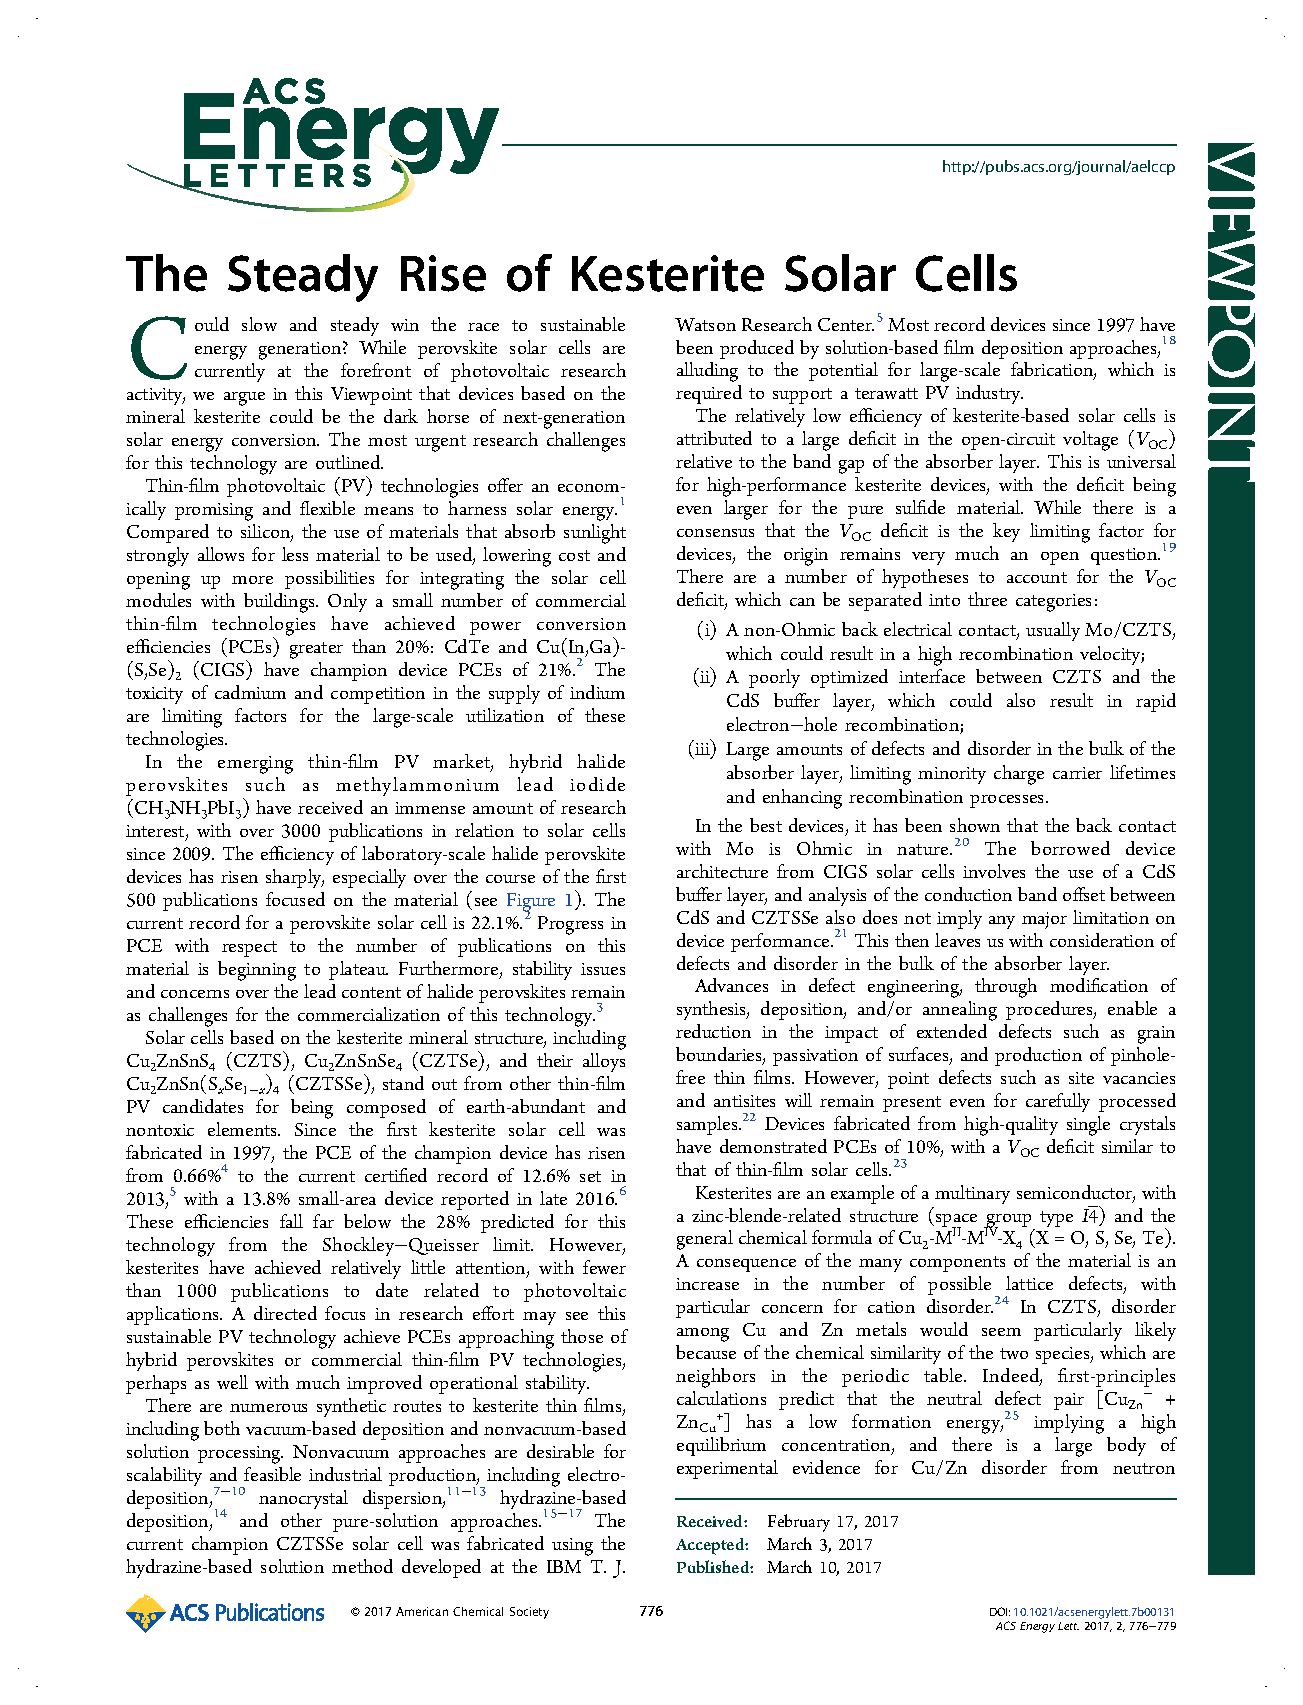
\includepdf[pages={1-},scale=1.0]{papers/CZTS_lett.pdf}


\section{Impact of defects on {\CZTS} solar cells}\label{CZTS_defects_lit}
Large amounts of defects and disorder in the bulk of the absorber layer was listed as one of the possible origins of the performance deficit of {\CZTS} solar cells in the letter presented in the previous section.
The low open circuit voltage (V$_{OC}$) relative to the band gap has been recognised as the key limiting factor on the performance of {\CZTS} solar cells \cite{culprit}. 
The measured current density-voltage (J-V) curve of a solar cell is used to determine the solar to electric power conversion efficiency (PCE), $\eta$. The PCE of a solar cell is the ratio of power output from the solar cell ($P_{MP}$) to the power input from the Sun ($P_{in}$). This is shown in Eq.~\ref{PV_efficiency}. $P_{MP}$ is given in terms of the V$_{OC}$ (the voltage from the J-V curve of the solar cell at J = 0) and the short-circuit current density, $J_{SC}$, (the current density on the J-V curve at V = 0) in Eq.~\ref{P_MP}.
For an efficient solar cell, it is desirable to have a high $J_{SC}$, a high $V_{OC}$ and a FF that is as close to 1 as possible.
\begin{equation} \label{P_MP}
P_{MP} = FFV_{OC}J_{SC}
\end{equation}
\begin{equation} \label{PV_efficiency}
\eta = \frac{P_{MP}}{P_{in}} = \frac{FFV_{OC}J_{SC}}{P_{in}}
\end{equation}

\begin{figure}[h!]
  \centering
    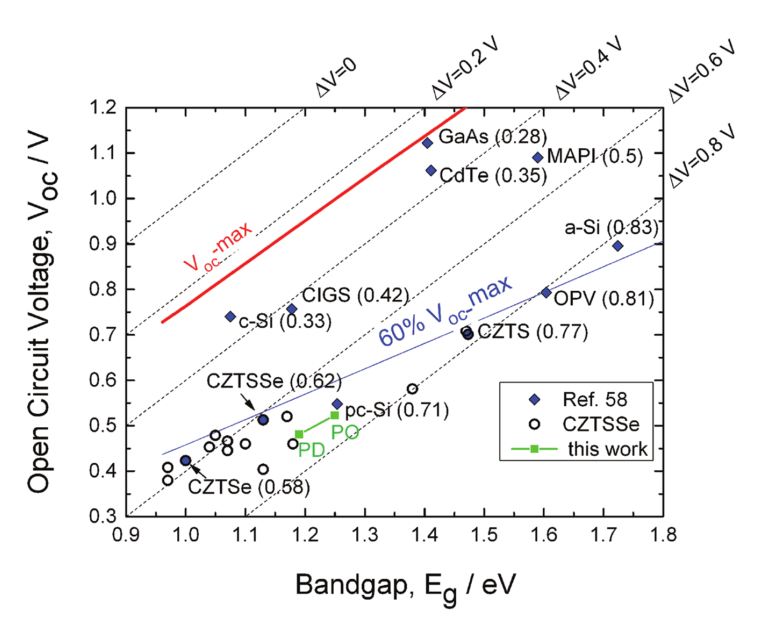
\includegraphics[width=0.85\textwidth]{figures/Voc.png}
    \caption[V$_{OC}$ versus band gap of high performance CZTSSe devices ($>$9\% efficiency) indicated by circles with best devices based on other photovoltaic materials shown for comparison by diamond symbols: Methyl-ammonium lead iodide (MAPI), amorphous silicon (a-Si), organic photovoltaic films (OPV), crystalline silicon (c-Si) and polycrystalline silicon (pc-Si). The oblique lines give a constant V$_{OC}$ deficit from 0.8 V to 0 V. The green points correspond to CZTSSe films that are partially ordered (PO) or partially disordered (PD) due to disorder amongst Cu and Zn.]{V$_{OC}$ versus band gap of high performance CZTSSe devices ($>$9\% efficiency) indicated by circles with best devices based on other photovoltaic materials shown for comparison by diamond symbols: Methyl-ammonium lead iodide (MAPI), amorphous silicon (a-Si), organic photovoltaic films (OPV), crystalline silicon (c-Si) and polycrystalline silicon (pc-Si). The oblique lines give a constant V$_{OC}$ deficit from 0.8 V to 0 V. The green points correspond to CZTSSe films that are partially ordered (PO) or partially disordered (PD) due to disorder amongst Cu and Zn. Figure reproduced with permission from Ref.~\citenum{culprit}.}
  \label{Voc}
\end{figure}

As can be seen from the position of CZTSSe devices on the plot in Fig.~\ref{Voc}, the V$_{OC}$ measured for these devices are considerably less than that of the higher-performing CIGS devices, which have a similar value for the band gap of the material.
In general, the main cause of V$_{OC}$ deficit in a PV device is the recombination of photogenerated charge carriers in the bulk material or at surfaces \cite{culprit}. In {\CZTS} one explanation that has been put forward is band tailing in the bulk \cite{band_tail}.

\begin{figure}[h!]
  \centering
    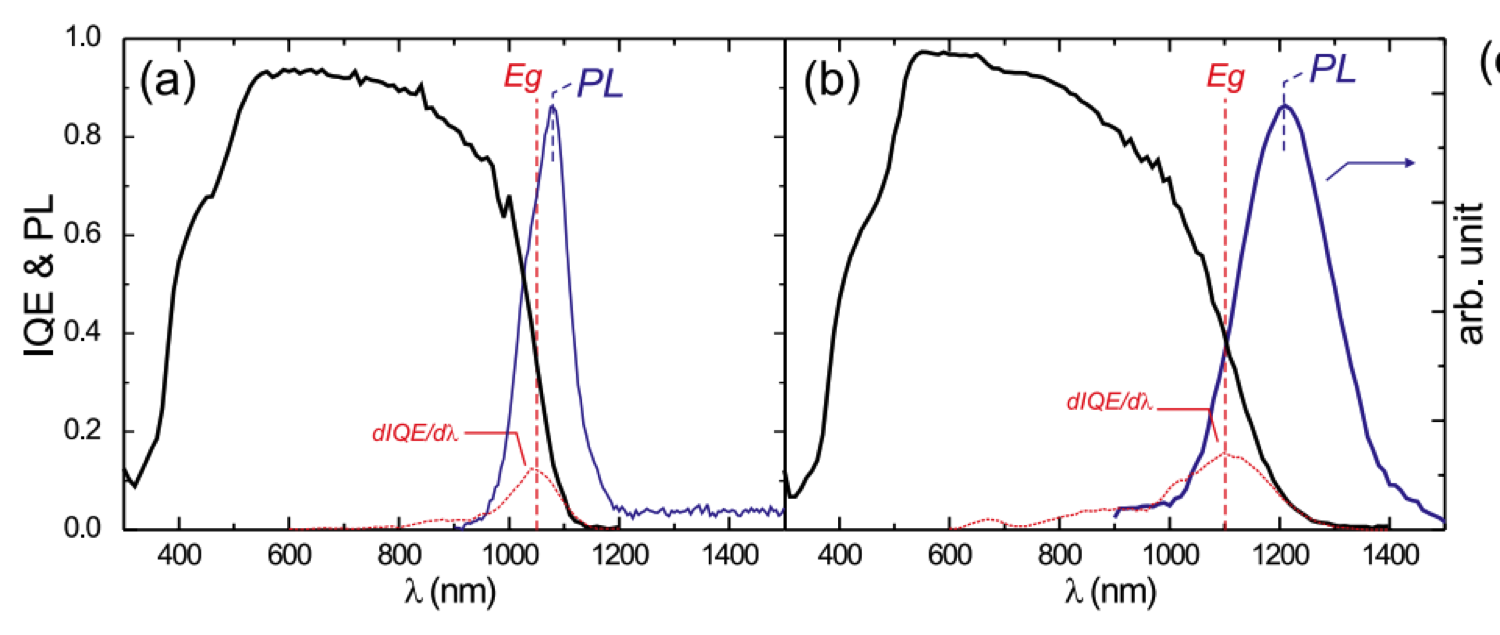
\includegraphics[width=1.0\textwidth]{figures/CZTS+CIGS_PL.png}
    \caption[The internal quantum efficiency (IQE), band gap as determined from the IQE inflection point and the photoluminescence spectra of high performance devices with thin-film absorber layers of (a) CIGSSe (E$_g$ = 1.19 eV) and (b) CZTSSe (E$_g$ = 1.13 eV).]{The internal quantum efficiency (IQE), band gap as determined from the IQE inflection point and the photoluminescence spectra of high performance devices with thin-film absorber layers of (a) CIGSSe (E$_g$ = 1.19 eV) and (b) CZTSSe (E$_g$ = 1.13 eV). Figure reproduced with permission from Ref.~\citenum{band_tail}.}
  \label{CZTS+CIGS_PL}
\end{figure}

Several PL studies have been performed on kesterite-structured samples of {\CZTS}, Cu$_2$ZnSnSe$_4$ and alloys of the two. PL measurements have been performed on both full devices and polycrystalline thin-films \cite{band_tail, Gershon, Gershon_ref18, Romero, Miyamoto, Unold} and single crystals \cite{Halliday, Levcenko, Hones}. Ref.~\citenum{Halliday} compares the PL spectra for varying compositions of the samples, whereas in Ref.~\citenum{band_tail} measurements on both CIGSSe and record-efficiency CZTSSe thin films are performed in an attempt to account for the difference in the performance of these two technologies by comparing their defect-influenced PL emission spectra. Polycrystalline samples are more similar to those likely to be used in thin-film CZTS photovoltaic devices, however, comparison between those measurements with single crystal measurements could enable the isolation of recombination at grain boundaries and interfaces from those due to defects in the bulk of the absorber layer. 
%Also measurements performed on single crystals as close to perfectly stoichiometric {\CZTS} as possible are likely to be the most directly relatable to our simulations on bulk systems. 
One feature common to all of the PL spectra from studies on kesterite samples is clear evidence of defects and disorder from the observed band tailing. 
Fig.~\ref{CZTS+CIGS_PL} shows PL spectroscopy measurements performed on CZTSSe thin films by Gokmen et al \cite{band_tail}. The figure shows that there is a shift in the PL peak to lower energies (red-shifting), below the value of the band gap obtained from internal quantum efficiency (IQE) measurements performed on the same thin films. It is also noted in this study when comparing the PL spectra of CZTSSe films to that of CIGSSe films that the PL peak for CZTSSe thin films is broader and that the red-shifting was roughly twice as severe. This effect is referred to as the `band-edge tailing', where photons of energies less than the band gap of the material are emitted following photoexcitation and subsequent relaxation back to the ground state. 
%This effect is known to be detrimental for device performance as emitted photons may then not have sufficient energy for subsequent photoexcitations in the absorber layer, the energy of the original photon may then not be converted into electricity if the photoexcited electron-hole pair recombine before the charge is collected \cite{Nelson4}.
%The PL spectra of kesterite samples usually features a much broader peak than that observed in CIGSSe samples, such as that shown in figure \ref{CZTS+CIGS_PL}. The energy of the maximum PL peaks of kesterite samples is also usually considerably red-shifted compared to the energy of the band gap. These two features are usually attributed to band tailing caused by either spatial band gap variations or electrostatic potential fluctuations in the absorber material.  Both effects lead to a non-zero density of states (DOS) within the band gap \cite{culprit, band_tail}. 
Measurements performed in Ref.~\citenum{band_tail} found the tailing in CZTSSe to be roughly twice as severe as that observed in higher-performing CIGSSe devices.

Theoretical predictions for the defect formation energy and defect transition levels in {\CZTS} in Ref.~\citenum{defects_Chen} suggest that defects which would be expected to produce a deep defect level also have a high formation energy and hence would be expected to be less likely to form.
However, a recent theoretical study has revisited the defect physics of {\CZTS} to demonstrate possible mechanisms where defect-mediated recombination could occur without a charge transition level deep in the band gap of the material \cite{Sunghyun_killer_defects}.
There is currently no experimental evidence on the nature of the defects that may be responsible for the latter, however, in {\CZTS} the presence of a large extent of disorder amongst Cu and Zn, and hence high concentrations of $Cu_{Zn}^{-}$ and $Zn_{Cu}^{+}$ antisites, has been inferred from calculations of defect formation energy \cite{defects_Chen} and confirmed from several experimental studies \cite{Schorr, CZTS_Xray, CZTS_TEM}. Although these types of defects are not predicted to produce a deep defect level or linked to the recombination mechanisms investigated in Ref.~\citenum{Sunghyun_killer_defects}, it has been proposed that they may be linked to observed band tailing in {\CZTS} due to the high-concentrations of the defects \cite{band_tail}.




\section{Defects beyond the dilute limit in {\CZTS}}\label{CZTS_beyond_dilute}
Electronic structure calculations for the formation energies of point defects and point defect pairs in the dilute limit have already been calculated for {\CZTS}, where the [$Cu_{Zn}^- + Zn_{Cu}^+$] defect pair was found to have a particularly low formation energy \cite{defects_Chen}.
The calculations performed in Ref.~\citenum{defects_Chen} were performed using the GGA functional with a rigid shift applied to the defect levels to account for the band gap error at this level of theory \cite{Lany_defects}. In Ref.~\citenum{defects_Chen} one defect calculation was performed using a hybrid functional where it was found that the formation energy of the test defect differed by 0.1 eV. This section of the thesis is concerned with the possible role of Cu/ Zn disorder in the performance deficit of {\CZTS} solar cells. We therefore repeated the calculation of the formation energy for the defect pair of interest for our study.

For our calculation of the formation energy of the nearest-neighbour [$Cu_{Zn}^- + Zn_{Cu}^+$] charge-neutral defect pair, we construct a 64-atom supercell from a $2\times2\times1$ expansion of the conventional unit cell of {\CZTS}. This was the most isotropic and largest supercell that could feasibly be used for our calculations at the level of theory desired.
The HSE06 hybrid-functional \cite{HSE} (described towards the end of section \ref{hse_theory}) was used for the exchange-correlation functional as implemented in the Vienna Ab-initio Simulation Package (VASP) \cite{VASP} with an energy cut-off of 500 eV for the plane-wave basis set during relaxation of the defect-pair supercell. Calculations were initially performed at the gamma point (a 1x1x1 \textit{k}-point mesh) until forces on the ions converged to within 0.01 eV/ $\AA$. 
A single geometry step was then performed with a 2x2x2 \textit{k}-point mesh centred on the gamma point as these parameters were found to be sufficient for the total energy to converge to within $<$2 meV per atom with respect to increased plane-wave cut-off energy and for the external pressure to be $<$1 kbar. However, performing the full calculation with a 2x2x2 \textit{k}-point mesh was found to be too computationally expensive. 
%Data for the convergence test is given is table \ref{conv_test}. 
As the defect pair is charge neutral, we were able to use Eq.~\ref{defect_neutral} to calculate the formation energy. From our calculation, we predict a defect formation energy of 0.30 eV. While the value from a previous study using a GGA functional was approximately 30\% less than this value at 0.21 eV \cite{defects_Chen}.

\begin{figure}[h!]
  \centering
    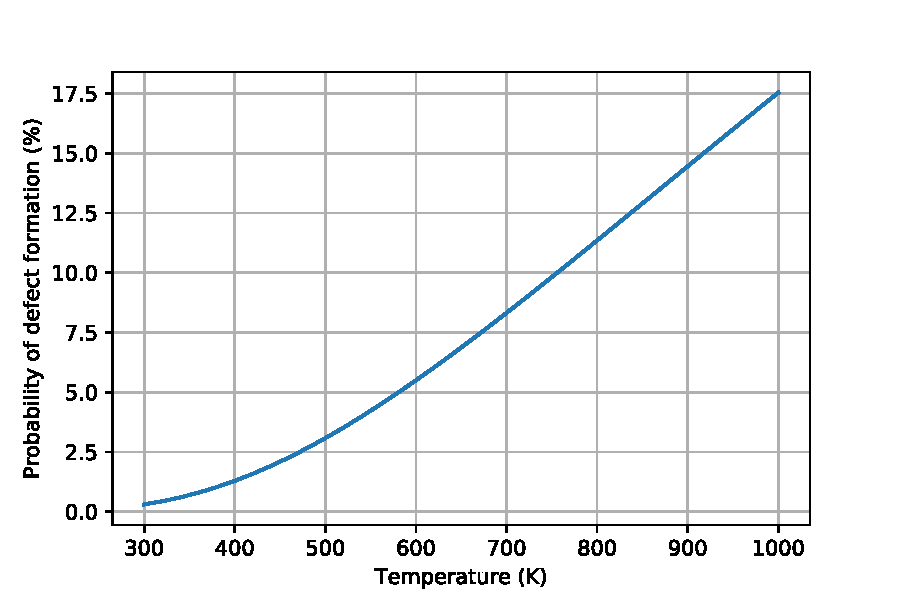
\includegraphics[width=0.9\textwidth]{figures/CZTS_Cu-Zn_defect_conc.pdf}
    \caption{Probability of nearest neighbour [$Cu_{Zn}^- + Zn_{Cu}^+$] defect formation as a function of temperature based on the equilibrium defect concentration from classical thermodynamics.}
  \label{Cu-Zn_eqm_conc}
\end{figure}

When defect concentrations are less than 1\%, it is usually assumed that the system is in the dilute defect limit where defects can be considered to be non-interacting \cite{Stoneham_defect_lim}. Using statistical thermodynamics for point defects, an expression for the equilibrium concentration of point defects as a function of temperature can be obtained \cite{thermodynamics}, as shown in Eq.~\ref{defect_conc}, where N is the number of sites, $\Delta H$ is the defect formation energy, $k_B$ is the Boltzmann constant and T is the temperature of the system. This expression will be discussed further in section \ref{enargite_defects}, but for now it is just applied to determine the regime of defect concentration we are dealing with for the present investigation.
\begin{equation} \label{defect_conc}
n = Ne^{\frac{-\Delta H}{k_BT}}
\end{equation}
The probability of defect formation as a function of temperature is given by the exponential expression in Eq.~\ref{defect_conc}. The defect formation energy from the DFT calculations were halved to take an average of the formation energy per defect during the formation of an antisite pair before being inserted into this expression. This is plotted against temperature in Fig.~\ref{Cu-Zn_eqm_conc}. 
Even `low-temperature' synthesis procedures for {\CZTS} use annealing temperatures over 600K \cite{low_T_CZTS}. It can be seen from Fig.~\ref{Cu-Zn_eqm_conc} that the probability of defect formation even at 600K is much higher than what would be considered as the `dilute limit'.
Furthermore, there is experimental evidence of high concentrations of Cu/ Zn disorder \cite{Scragg, pot_fluc_4, neutron, Schorr}, indicating the likely formation of extended defect structures beyond point defects and pairs. To simulate such defect structures in {\CZTS} a bespoke Monte Carlo model was developed. This will be outlined in the next section and is applied in the study presented in section \ref{CZTS_MC} \cite{eris_paper}.


\subsection{Monte Carlo model for Cu/ Zn disorder in {\CZTS}}\label{Eris}
The general methodology for simulating thermodynamic substitutional disorder with the Metropolis Monte Carlo scheme was introduced in section \ref{MC}. The on-lattice Monte Carlo model developed here to simulate thermodynamic Cu/ Zn disorder is analogous to the Ising model of a ferromagnet, descriptions of which can be found in many textbooks such as Ref.~\citenum{MC} and \citenum{MC_Landau}. 
The Ising model uses interactions between spins, whereas our model considers the Coulombic interaction between the bare formal charges of ions in the lattice of {\CZTS}.
In the case of an Ising model, the trial moves in the Metropolis algorithm are spin flips, whereas in our model the trial moves are swaps between nearest-neighbour Cu and Zn ions. Typically, when performing simulations of an Ising model the calculated quantities of interest are the internal energy and average magnetisation of the system as a function of temperature obtained by summing over the distribution of atomic spins. In the case of our system, the quantities of interest are the spatial arrangement of the Cu and Zn ions due to thermodynamic substitutions between the two species and the resulting distribution of electrostatic potential across the system.
%for the implications this could have on band tailing. 

\begin{figure}[h!]
  \centering
    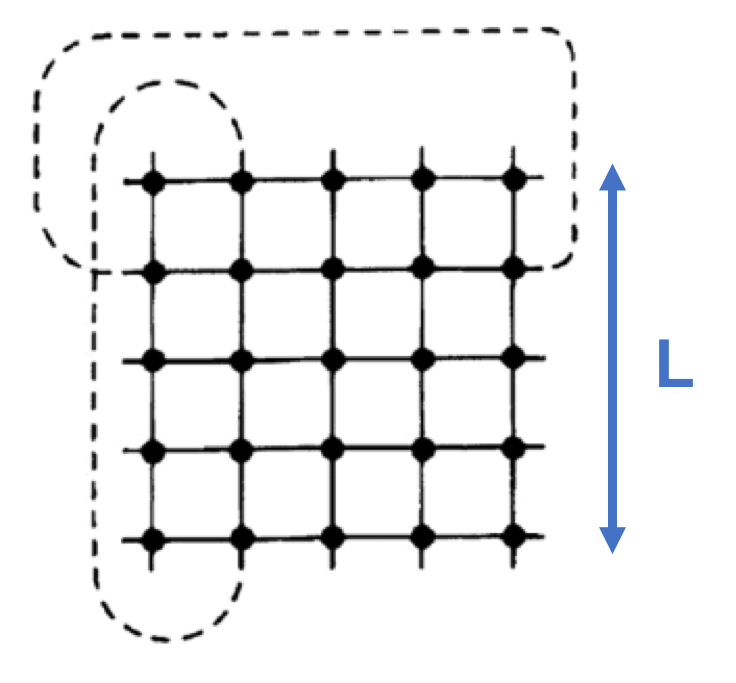
\includegraphics[width=0.4\textwidth]{figures/MC_PBCs.png}
    \caption[Typical periodic boundary conditions for the two-dimensional Ising model.]{Typical periodic boundary conditions for the two-dimensional Ising model. Figure reproduced with permission from Ref.~\citenum{MC_Landau}.}
  \label{MC_PBCs}
\end{figure}

Before we attempt to extract any information on thermodynamic disorder, two important considerations for our model will be: to determine if the disordered configuration we obtain is in fact the equilibrated configuration at the given simulation temperature and secondly if finite size effects are having an impact on the system properties we obtain from our simulations.
As simulations are performed for finite lattices, to simulate a bulk system the edges or `boundaries' of the system must be treated carefully. The boundaries can be effectively eliminated through the use of periodic boundary conditions (PBCs). In the case of an Ising model, this means that the first spin in a row interacts with the last spin in the row as if it were a nearest neighbour, and vice versa \cite{MC_Landau}. This principle is illustrated for a two-dimensional system in Fig.~\ref{MC_PBCs}. Although this procedure effectively eliminates boundary effects, the system is still characterized by the finite lattice size, L, which limits the correlation length to $\frac{L}{2}$. Resultant properties of the simulated system may then differ from the bulk system. We therefore will need to perform simulations with increasing system size to look for any differences in the quantities of interest.

Determining if our system has reached equilibration at each temperature, however, may require a more complicated procedure. As the Monte Carlo method is stochastic, making use of sampling many times with random numbers to determine the minimum energy configuration of the system, the trajectory to reach this final configuration will by nature be random. Therefore, we can draw no conclusions about the properties of our system from evolved states until the final configuration at the particular temperature is reached. Methods were developed and tested to check for equilibration before attempting to extract any thermodynamic properties of our system.

\begin{figure}[h!]
  \centering
    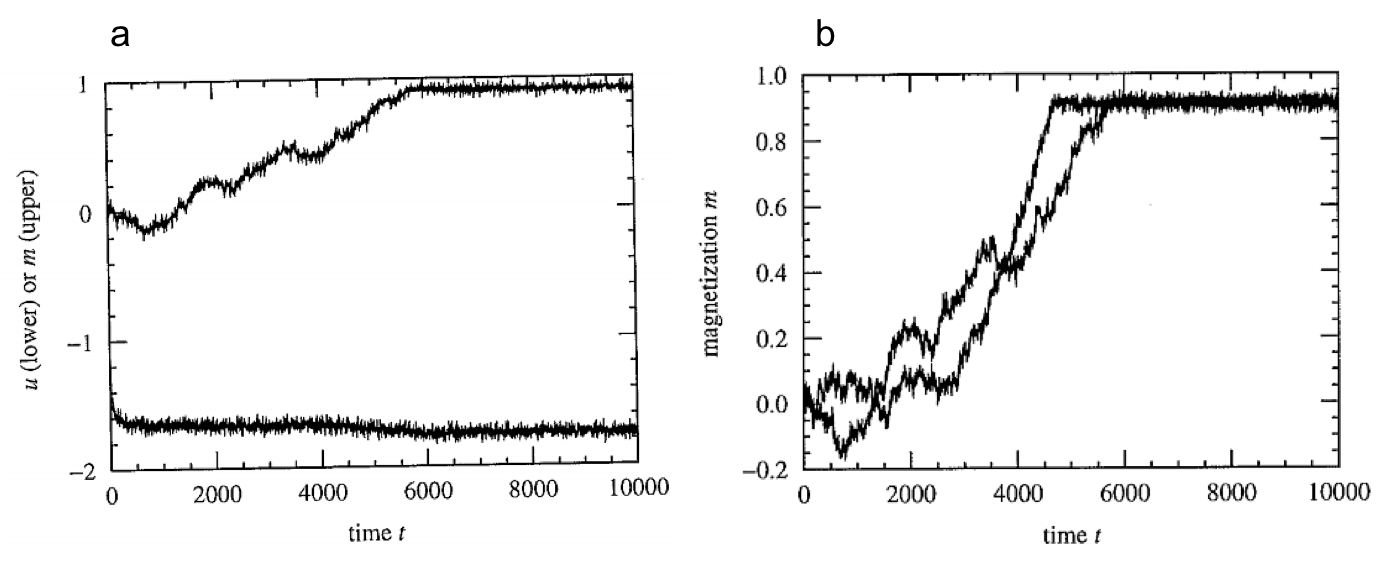
\includegraphics[width=0.9\textwidth]{figures/ising_equil.png}
    \caption[The magnetisation (upper curve) and internal energy (lower curve) per site of a two-dimensional Ising model simulated using the Metropolis algorithm (a). Magnetisation as a function of time for two different simulations (b). Time is measured in Monte Carlo steps per lattice site.]{The magnetisation (upper curve) and internal energy (lower curve) per site of a two-dimensional Ising model simulated using the Metropolis algorithm (a). Magnetisation as a function of time for two different simulations (b). Time is measured in Monte Carlo steps per lattice site. Figure reproduced with permission from Ref.~\citenum{MC}.}
  \label{ising_equil}
\end{figure}

In the case of the Ising model when, for example, determining the average magnetisation of a system at a given temperature, the simulation must be run for a suitably long time until the system has come to equilibrium at that temperature. This is referred to as the equilibration time. 
%Once the system has equilibrated, the quantity of interest, such as the magnetisation, must then be measured again over a suitably long time and averaged. 
To gauge if a system has reached equilibrium, in the case of the Ising model, it is common practice to run the simulation for a large number of Monte Carlo steps (MCS) (where one MCS corresponds to attempting a trial spin-flip at all sites in the system once) and looking for how the value of a quantity of interest, such as the average magnetisation across the system, changes with increasing number of MCS as the simulation progresses. Equilibration is often considered as the point at which the value of a quantity of interest, which initially changes by a large amount, eventually converges to fluctuating about a steady average value. An example of this is shown in Fig.~\ref{ising_equil}a. This is dependent upon the principle that a system in equilibrium spends the overwhelming majority of its time in a small subset of states in which its properties take a narrow range of values \cite{MC}. Provided the simulation has equilibrated, the final configuration for a given system at a given temperature should always be the same regardless of the initial configuration of the simulation, this point is illustrated in Fig.~\ref{ising_equil}b.

\begin{figure}[h!]
  \centering
    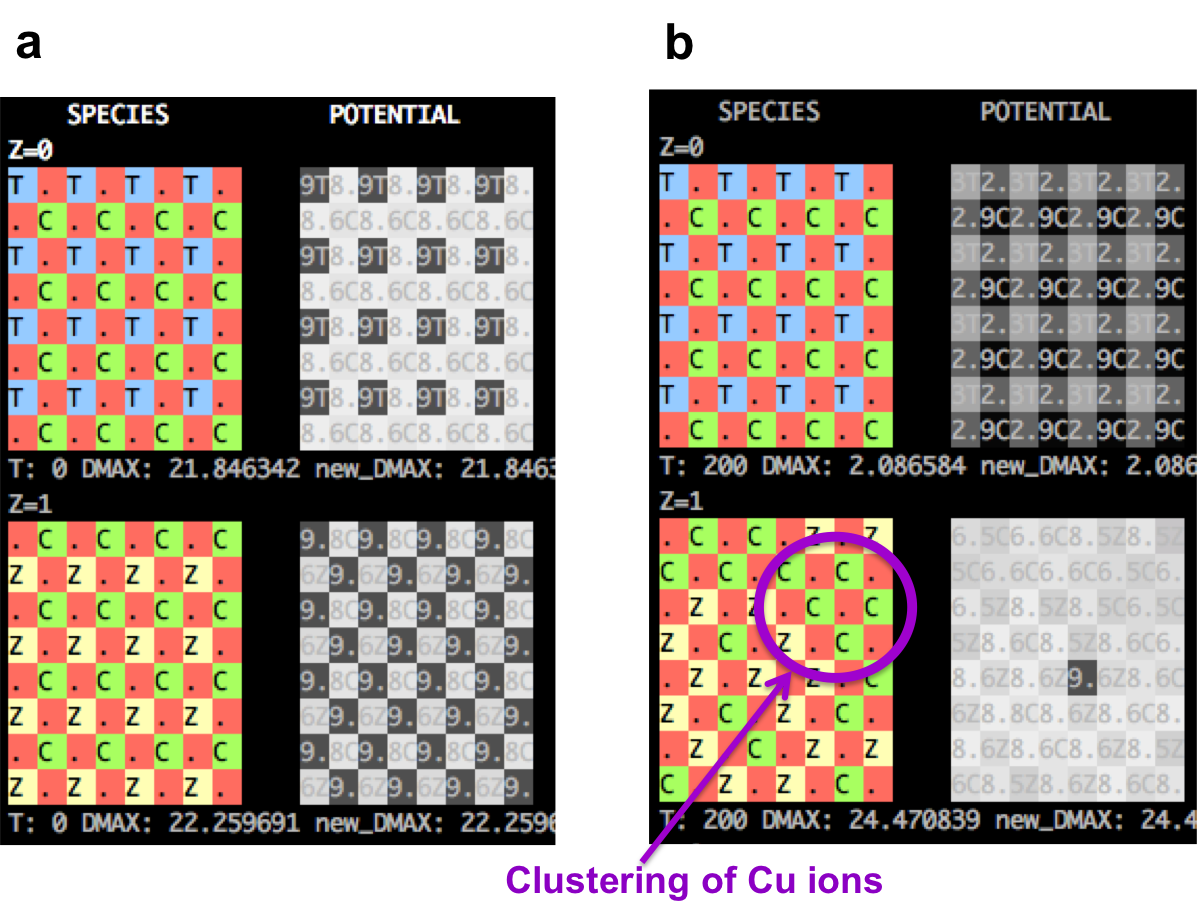
\includegraphics[width=0.9\textwidth]{figures/eris_spatial_disorder.png}
    \caption{Example outputs of 2D slices of cation sub-lattice of {\CZTS} from Eris Monte Carlo simulations of Cu-Zn disorder from an initially ordered lattice showing the top two layers of the lattice when simulations are performed at temperatures T = 0K (a) and at sufficiently high temperatures for Cu-Zn substitutions (b).}
  \label{eris_spatial_disorder}
\end{figure}

Using this principle, one way to determine if our system has reached its equilibrium configuration could be to use perfectly ordered or disordered initial lattice configurations. Both of these initial configurations, if the simulation is allowed to evolve over a suitable number of MCS, should eventually result in the same equilibrium system configuration. It would be difficult to distinguish differences in the atomic arrangement of one 3D lattice to another by eye, therefore comparisons of the pair correlation functions (PCFs) for each configuration as it evolves from either an ordered or disordered initial configuration can be made. 
Another method to check for equilibration is analogous to that shown in Fig.~\ref{ising_equil}a for the Ising model. In the case of our system, it is the distribution of on-site electrostatic potentials in the system that is of interest. As we fix Sn ions in our simulation, we calculate the on-site electrostatic potential for Sn ions to study how the chemical environment of these species is altered by Cu/ Zn disorder. To check for equilibration, we look for a point after which the variance of the distribution of electrostatic potentials of Sn ions across the system has reached a steady value. Both of these methods were tested and are discussed in the study in section \ref{CZTS_MC} \cite{eris_paper}.

Monte Carlo simulations of thermodynamic substitutions between Cu and Zn ions will be allowed to evolve until the equilibrium configuration in terms of the arrangement of Cu and Zn atoms at the given temperature is reached. Fig.~\ref{eris_spatial_disorder} shows an example output from our simulations, where Fig.~\ref{eris_spatial_disorder}a shows a perfectly ordered system at T = 0K and Fig.~\ref{eris_spatial_disorder}b shows spatial clustering of Cu and Zn ions as the system has been allowed to evolve at a finite temperature. The model is used to investigate and quantify thermodynamic Cu/ Zn disorder in {\CZTS} in the study presented in the next section. 
%The electrostatic potential at each site in the lattice in disordered configurations can be calculated for later analysis of the distribution of electrostatic potential across the system due to Cu-Zn disorder. This will discussed further in section \ref{eris_band_tailing}. 




\subsection{Publication: Atomistic insights into the order-disorder transition in {\CZTS} from Monte Carlo simulations}\label{CZTS_MC}
For {\CZTS} a lot of attention in the literature has been paid to disorder amongst Cu and Zn cations with a large amount of experimental evidence for the presence of this disorder \cite{Schorr, CZTS_Xray, CZTS_TEM} and theoretical predictions for the low formation energy of the  $[Cu_{Zn}^{-} + Zn_{Cu}^{+}]$ antisite pair \cite{defects_Chen}.
%During the synthesis of {\CZTS}, temperatures above room temperature are used and it is possible for some of the thermal disorder associated with the system at higher temperatures to be `frozen in' to the material as it cools to room temperature.
Near resonant Raman spectroscopy has been used to examine thin films of {\CZTS} prepared using different thermal treatments to determine if long post-annealing cooling times could produce films with a high level of order amongst Cu and Zn cations. In this study the authors postulate that achieving a very high level of order amongst Cu and Zn could require years \cite{Katharina}. This clearly would not be a practical treatment for a PV device and so it would seem that the presence of a fairly large amount of disorder amongst Cu and Zn, and hence $Cu_{Zn}^{-}$ and $Zn_{Cu}^{+}$ antisites,  is inevitable in the material. 

In the following paper, we have applied a bespoke Monte Carlo model to gain atomistic insights into the spatial distribution of thermodynamic disorder on Cu and Zn sites in the cation sublattice. 
Cation site disorder averaged over a macroscopic sample (as is probed from measurements) does not provide insights into the microscopic cation distribution that will interact with photogenerated electrons and holes.
In this study we consider 2D Cu/ Zn disorder, involving just substitutions amongst the cations in Cu-Zn (001) planes, and 3D Cu/ Zn disorder, where Zn ions may also substitute onto Cu 2\textit{a} sites in Cu-Sn (001) planes. 
Previous experimental studies have suggested that 2D Cu/ Zn disorder is the dominant disorder mechanism for the Cu/ Zn order-disorder transition (ODT) and that disorder on Cu 2\textit{a} sites only occurs after the ODT \cite{disorder_july}. However, more recent studies have suggested that this disorder mechanism is a part of the ODT \cite{Cu2a_expt, Cu2a_theory}.
We extract the critical temperatures, T$_C$, for the Cu/ Zn ODT for these two Cu/ Zn disorder mechanisms. We find that defects are less concentrated in Cu-Sn (001) planes but that Zn ions readily substitute into Cu-Sn planes even before the ODT and present spatial distributions of antisites from thermodynamic Cu/ Zn disorder in our model.

%The supplemental material for this paper is included in Appendix \ref{eris1_appendix}.


\includepdf[pages={1-},scale=1.0]{papers/Eris1_soa.pdf}

%\subsection{**Statement of authorship}
%The Bespoke Monte Carlo model, Eris, (doi: 10.5281/zenodo.1248445) developed for this publication is based on the Starry Night code (doi: 10.5281/zenodo.10543) written by Jarvist Moore Frost (JMF) to simulate dipole-dipole interactions and ferroelectric domains in a hybrid organic-inorganic perovskite solar cell. Eris was originally adapted by JMF from Starry Night to simulate thermodynamic Cu-Zn disorder in {\CZTS}. My personal contributions to the project involved both implementation and of development of the Eris code. Contributions from implementation of the code include running simulations to test for finite size effects in the model, generating data and developing post-processing tools to quantify and visualise Cu-Zn disorder in the system. My developments of the Eris code include writing routines for:
%\begin{itemize}
%    \item Lattice initialisation methods to ensure a stoichiometric {\CZTS} crystal
%    \item Testing the convergence in the electrostatic summations for calculating the change in lattice energy when performing a Monte Carlo move
%    \item Developing and testing methods to check that the equilibrium disordered configuration was achieved for each simulation temperature
%    \item Additional outputs from the code including: data to compute an order parameter, tests for convergence when computing on-site electrostatic potentials and outputting lattice on-site electrostatic potentials in various forms for further analysis
%    \item Extending the model to include Cu/Zn disorder between the planes, i.e. allowing Zn from Cu-Zn layers to substitute onto Cu sites in the Cu-Sn planes
%\end{itemize}
%Support and discussions were provided by Jarvist Moore Frost and Aron Walsh throughout this study.

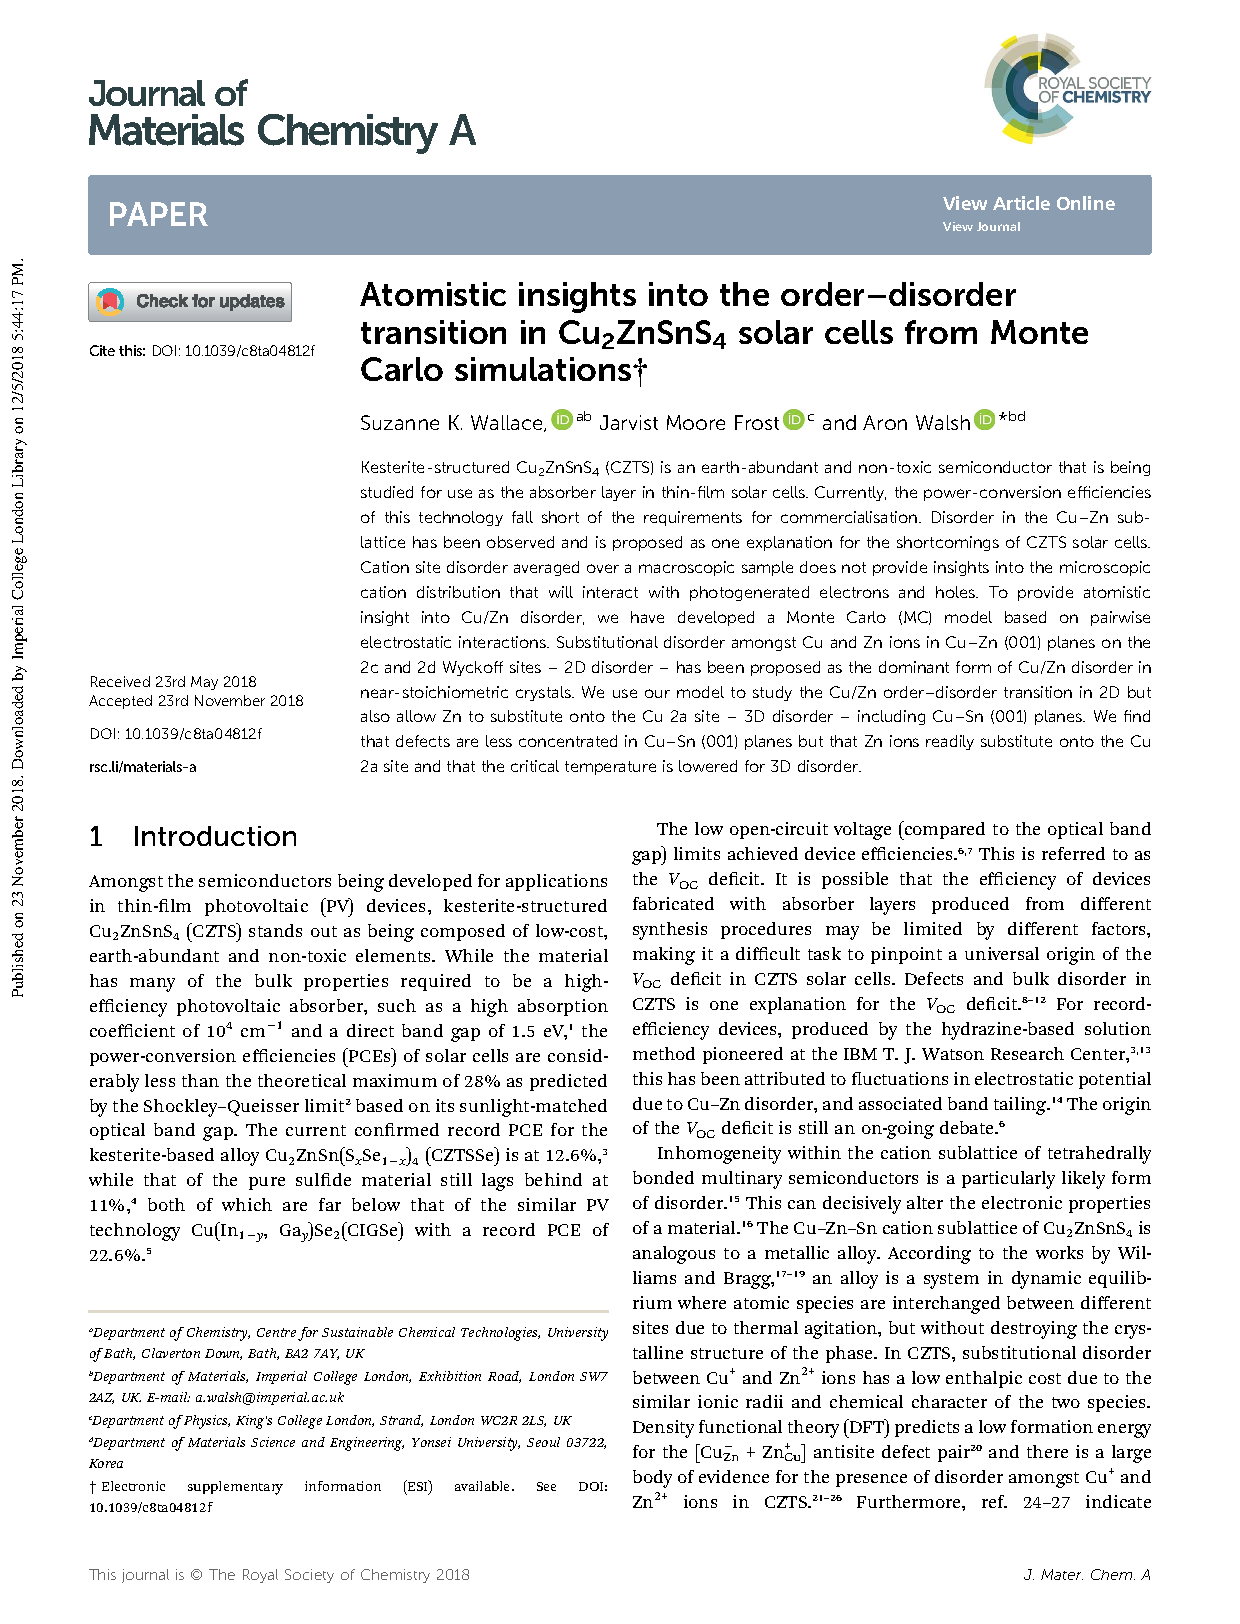
\includepdf[pages={1-},scale=1.0]{papers/eris_paper.pdf}




%\section{Outlook: Band tailing and modified defect physics from Cu-Zn disorder}
%\section{Outlook: Impact of Cu-Zn disorder on solar cell performance}\label{eris_future_work}
\section{Electronic band tailing in {\CZTS}}\label{eris_band_tailing}
Electronic band tailing was introduced in section \ref{defect_theory} and is associated with large extents of disorder and inhomogeneity in an absorber layer. It can be caused by either spatial band gap variations or electrostatic potential fluctuations in the material \cite{band_tail} indicated in Fig.~\ref{gokmen_band_tailing}a and \ref{gokmen_band_tailing}b respectively. In the case of the former, for example, an impurity atom of a different size to the atoms of the host lattice can result in a local mechanical strain, as shown in Fig.~\ref{pankove_band_fluc}b, which results in a deformation potential, such as that shown in Fig.~\ref{pankove_band_fluc}c for an edge dislocation defect. Local strains can alter the separation of atoms in the crystal and, as Fig.~\ref{pankove_band_fluc}a shows, the atomic separation within a crystal has a significant impact on the band structure. Additionally, due to the narrow region of phase stability for {\CZTS}, it is also possible there may be compositional inhomogeneity and secondary phases present \cite{SandS}, which could also produce local band gap fluctuations.

\begin{figure}[h!]
\centering
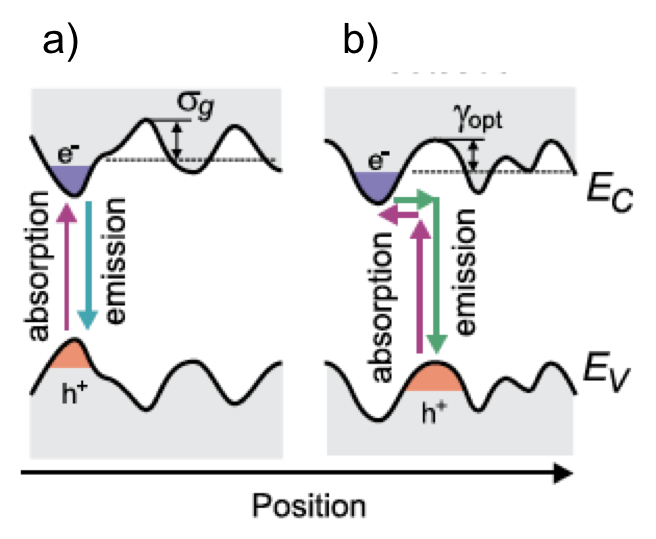
\includegraphics[width=0.6\textwidth]{figures/gokmen_band_tailing.png}
\caption[Schematic of band gap fluctuations (a) and electrostatic potential fluctuations (b) where the band gap is only maintained in the case of (b).]{Schematic of band gap fluctuations (a) and electrostatic potential fluctuations (b) where the band gap is only maintained in the case of (b). Figure reproduced with permission from Ref.~\citenum{band_tail}.}\label{gokmen_band_tailing}
\end{figure}

\begin{figure}[h!]
  \centering
    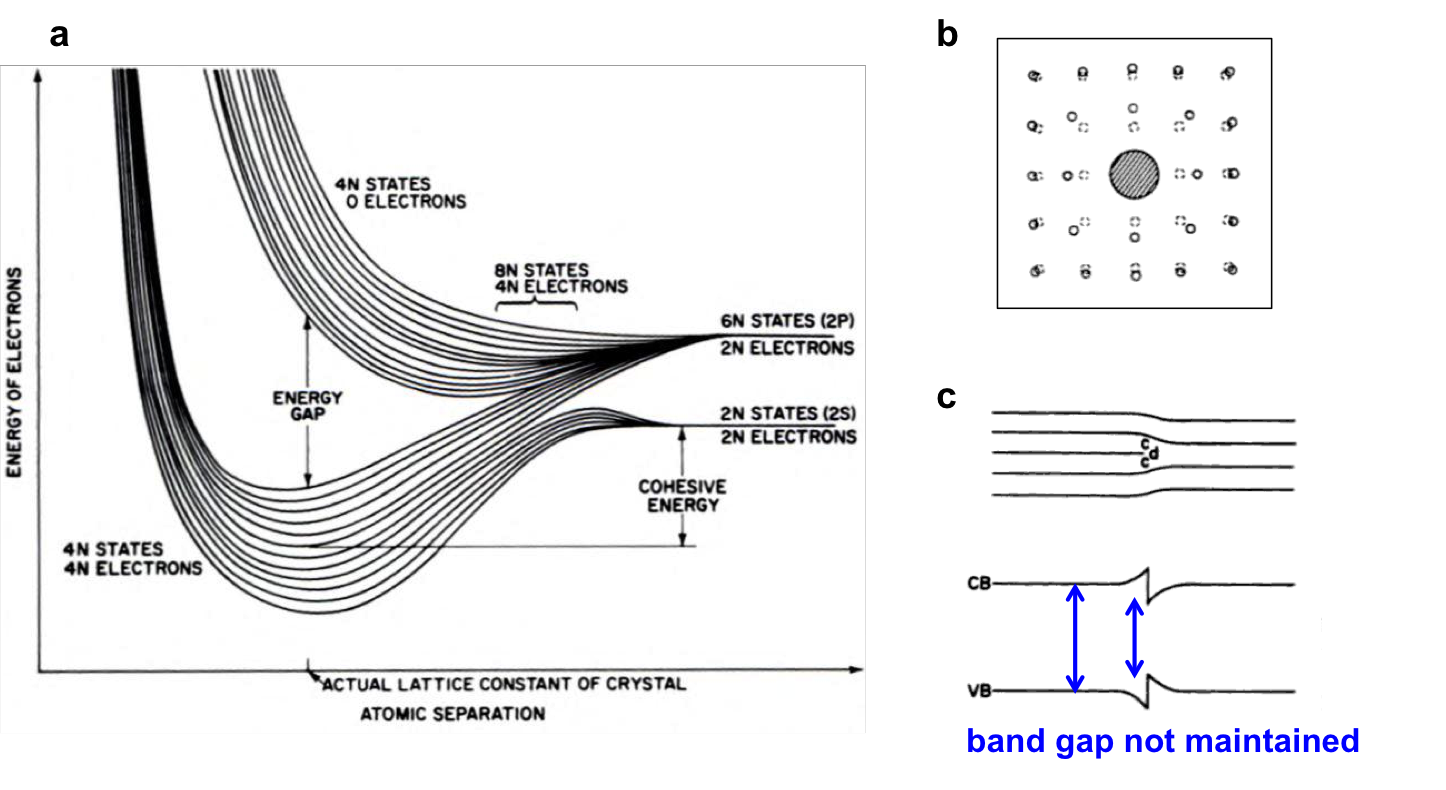
\includegraphics[width=1.0\textwidth]{figures/pankove_band_fluc.png}
    \caption[Energy banding of allowed levels in diamond as a function of spacing between atoms (a). Compressional strain induced in a crystal lattice by the incorporation of a large impurity atom (b). Deformation potential in the band structure due to compressional and dilational strain from an edge dislocation defect (c).]{Energy banding of allowed levels in diamond as a function of spacing between atoms (a). Compressional strain induced in a crystal lattice by the incorporation of a large impurity atom (b). Deformation potential in the band structure due to compressional and dilational strain from an edge dislocation defect (c). Figure reproduced with permission from Ref.~\citenum{Pankove} and adapted.}
  \label{pankove_band_fluc}
\end{figure}

In the case of electrostatic potential fluctuations, it is the inhomogeneous distribution of ionised defects that cause the fluctuations. An ionised donor exerts and attractive force on conduction electrons and a repulsive force on valence holes. As the defects are distributed randomly, the local interaction varies depending on the crowding of the defects. In this case the energy gap between the valence band and conduction band is maintained, as shown in Fig.~\ref{gokmen_band_tailing}b, and the states of each tail are spatially separated \cite{Pankove}. The broadening of the PL peak measured for {\CZTS} has been attributed to spatially fluctuating electrostatic potential in the material \cite{CZTS_TEM}.

%\begin{figure}[h!]
%  \centering
%    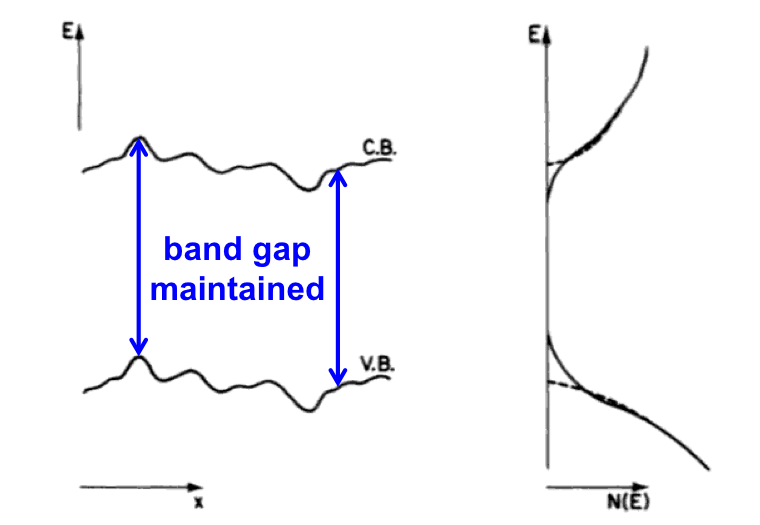
\includegraphics[width=0.6\textwidth]{figures/pankove_elec_fluc.png}
%    \caption[The perturbation of the band edges by Coulomb interaction with inhomogeneously distributed impurities (left), leading to the formation of tail states (right). Dashed lined show the distribution of states in the unperturbed case]{The perturbation of the band edges by Coulomb interaction with inhomogeneously distributed impurities (left), leading to the formation of tail states (right). Dashed lined show the distribution of states in the unperturbed case. Fig.~taken from Ref.~\citenum{Pankove} and adapted.}
%  \label{pankove_elec_fluc}
%\end{figure}


%Point defects in an otherwise perfect lattice can be regarded as missing lattice atoms, which are replaced by lattice defects. Therefore for every defect that creates one or more levels in the band gap of the material, the same number of levels that would have been created by the atoms in the host lattice are missing. Additionally, the lattice atoms surrounding the defect relax into shifted positions and also create states that could be shifted slightly into the band gap \cite{thin_film_Boer}. All of these states contribute to perturbations in the band edge relative to that of a perfect material, such as that shown in Fig. \ref{pankove_elec_fluc}. 

%As discussed in section \ref{CZTS_beyond_dilute}, concentrations of $[Cu_{Zn}^{-} + Zn_{Cu}^{+}]$ antisites in {\CZTS} are expected to be beyond the dilute limit. As outlined in section \ref{CZTS_defects_lit}, severe electronic band tailing has been observed experimentally in {\CZTS} \cite{band_tail, kesterite_band_tails}. 

%In this section, we use lattice configurations of tens of thousands of atoms with equilibrium thermodynamic Cu/ Zn substitutional disorder from our Monte Carlo model to quantify the contribution to electronic band tailing in {\CZTS} from the spatial fluctuations in electrostatic potential due to the high concentration of $[Cu_{Zn}^{-} + Zn_{Cu}^{+}]$ antisites. 



\subsection{Fluctuations in electrostatic potential from Monte Carlo simulations of Cu/ Zn disorder}

Disordered lattice configurations generated from the study presented in section \ref{CZTS_MC} \cite{eris_paper} could be used to infer the possible contribution to electronic band tailing in {\CZTS} from potential fluctuations caused by high concentrations of charged $Cu_{Zn}^{-}$ and $Zn_{Cu}^{+}$ antisite defects. 
It is worth noting that fluctuations in electrostatic potential are not the only possible contribution to band tailing, as discussed in the previous section, and that our model cannot account for any strain effects on the band gap (shown in Fig.~\ref{pankove_band_fluc}) because it is fixed on-lattice. However, there are differing views in the literature as to whether it is electrostatic potential fluctuations or band gap fluctuations from Cu/ Zn disorder that is the main contribution to the observed band tailing and the performance deficit of {\CZTS} solar cells, or, if Cu/ Zn disorder is the main bottleneck to improving device efficiencies at all \cite{culprit, kesterite_band_tails, band_tail}. As our model considers only one contribution, we would be able to isolate the possible impact of this specific contribution.

\begin{figure}[h!]
  \centering
    \includegraphics[width=0.85\textwidth]{figures/CZTS_band_structure.png}
    \caption[Electronic band structure of {\CZTS} calculated with the HSE06 hybrid-DFT functional, total and partial density of states, and schematic plot of the band components.]{Electronic band structure of {\CZTS} calculated with the HSE06 hybrid-DFT functional, total and partial density of states, and schematic plot of the band components. Figure reproduced with permission from Ref.~\citenum{defects_Chen_large}.}
  \label{CZTS_band_structure}
\end{figure}

To quantify the contribution to electronic band tailing from fluctuations in electrostatic potential caused by $[Cu_{Zn}^{-} + Zn_{Cu}^{+}]$ antisites, the distribution of on-site electrostatic potentials of species in the disordered lattice configurations obtained from our Monte Carlo model could be used to infer perturbations to the band edges compared to the perfect, bulk material. In the study presented in section \ref{CZTS_MC} \cite{eris_paper}, we showed that 3D Cu/ Zn disorder was an important mechanism in the Cu/ Zn ODT, we therefore would use configurations generated from our Monte Carlo model with 3D Cu/ Zn disorder. The electronic band structure of {\CZTS} and composition of the frontier orbitals is shown in Fig.~\ref{CZTS_band_structure}. 
The VBM of {\CZTS} is formed from the hybridisation of Cu-3d and S-3p orbitals, while the CBM is formed from the hybridisation of Sn-5s orbitals with S-3p and 3s \cite{defects_Chen_large}. Due to the composition of the frontier orbitals of {\CZTS}, the potential distribution of Cu and Sn ions from our model could be used to infer band tailing of the VBM and CBM respectively from fluctuations in electrostatic potential.

\begin{figure}[]
  \centering
    \includegraphics[width=1.0\textwidth]{figures/pot_dists.png}
    \caption{Distributions of on-site electrostatic potentials of Sn (top panels) and Cu (bottom panels) with increasing simulation temperature (left to right). The distribution broadens from one delta function for Sn ions at T=0K (corresponding to one crystallographically distinct Sn site) and broadens from two delta functions for Cu at T=0K corresponding to the Cu 2\textit{a} and 2\textit{c} sites in {\CZTS}.}
  \label{pot_dists}
\end{figure}

Fig.~\ref{pot_dists} shows the impact of increased Cu/ Zn disorder on the distribution electrostatic potentials of Sn and Cu ions in the disordered lattice configurations obtained from our model. 
On-site electrostatic potentials are calculated by a summation over pairwise electrostatic interactions in the lattice using the bulk dielectric constant of {\CZTS} calculated in Ref.~\cite{Sunghyun_dielectric} to account for screening of the bare formal charges of ions by the surrounding material.
The top panel of Fig.~\ref{pot_dists} shows the change in the distribution of Sn potentials with increased simulation temperature from left to right and the bottom panel shows the same for Cu ions. In the case of Sn, the distribution broadens from a single delta function for the one crystallographically distinct Sn site in perfect kesterite {\CZTS}, while the lower panel for Cu shows the broadening of two delta functions with disorder for the Cu 2\textit{a} and 2\textit{c} sites in {\CZTS}.



%\begin{figure}[h!]
%  \centering
%    \includegraphics[width=0.95\textwidth]{figures/eris_vs_gulp.png}
%    \caption[Difference between the change in on-site potential per ion between a perfect host lattice of {\CZTS} and a host lattice with a single antisite defect pair for system sizes of $4\times4\times4$, $8\times8\times8$ and $12\times12\times12$ ions when calculated without an Ewald summation and when calculated with the General Utility Lattice Program.]{Difference between the change in on-site potential per ion between a perfect host lattice of {\CZTS} and a host lattice with a single $[Cu_{Zn}^{-} + Zn_{Cu}^{+}]$ antisite defect pair for system sizes of $4\times4\times4$, $8\times8\times8$ and $12\times12\times12$ ions when calculated without an Ewald summation and when calculated with the General Utility Lattice Program \cite{gulp}.}
%  \label{eris_vs_gulp}
%\end{figure}

%The calculation of on-site electrostatic potentials with the model used in the study presented in section \ref{CZTS_MC} \cite{eris_paper} involved a summation of all pairwise interactions over the lattice but does not make use of an Ewald summation for computing long-range interactions with periodic boundary conditions. We therefore first compare results obtained for on-site potentials for a perfect lattice and a system containing one antisite defect pair for increasing lattice sizes with our model to the General Utility Lattice Program (GULP) \cite{gulp} which does use an Ewald summation.

\begin{figure}[]
  \centering
    \includegraphics[width=0.95\textwidth]{figures/spatial_pot_Cu-Sn_950K_edit.png}
    \caption{2D histograms showing on-site electrostatic potentials in units of V for Cu (a) and Sn (b) in a (001) Cu-Sn plane minus the average on-site potential for each species within the same plane in our {\CZTS} lattice model for complete ($S=0$) equilibrium thermodynamic Cu/ Zn disorder at 950K. Any deviation from 0 potential demonstrates the spatial fluctuation in electrostatic potential across the plane and empty sites in (a) show where Zn ions have substituted onto Cu 2\textit{a} sites.}
  \label{spatial_pot_fluc_Cu-Sn}
\end{figure}

%Fig.~\ref{eris_vs_gulp} shows the difference between the change in on-site potential per ion between a perfect host lattice and a host lattice with a single $[Cu_{Zn}^{-} + Zn_{Cu}^{+}]$ antisite defect pair with system size increased from $4\times4\times4$, $8\times8\times8$, up to $12\times12\times12$ ions when calculated by our model and when calculated by GULP. The difference between values calculated with our model and with GULP for the same lattices shows a clear decrease with increased lattice size and appears to approach a plateau below 0.01V for the $12\times12\times12$ lattice, which is considerably smaller than the systems studied in section \ref{CZTS_MC} \cite{eris_paper}. A difference between our model and GULP could also be expected for very small lattices due to possible image interactions between the defects and their periodic images in calculations with GULP. From this we could expect that the error from not using an Ewald summation in our model when calculating on-site potentials would be of the order of 0.01V or less.

%The results presented in this section are obtained with on-site electrostatic potentials calculated from our model using the bulk dielectric constant of {\CZTS} calculated in Ref.~\cite{Sunghyun_dielectric} to account for screening of bare formal charges of the ions by the surrounding material. However, to correctly represent the screening of charges in the lattice would require a description of the local response of the electron density to an inhomogeneity in the lattice. The results are therefore just preliminary and further work is required to obtain a quantitative description of on-site potentials in the system.

Fig.~\ref{spatial_pot_fluc_Cu-Sn} shows the on-site electrostatic potentials of Cu and Sn in a (001) Cu-Sn plane minus the average on-site potential for each species within the same plane in our {\CZTS} lattice model for complete ($S=0$) equilibrium thermodynamic Cu/ Zn disorder at 950K. In Fig.~\ref{spatial_pot_fluc_Cu-Sn}a, a region with a clustering of $Zn_{Cu}^{+}$ antisites is indicated and Fig.~\ref{spatial_pot_fluc_Cu-Sn}b shows a corresponding increase in the local electrostatic potential of neighbouring Sn ions in the same plane. This is consistent with observations of clusters of $Zn_{Cu}^{+}$ antisites from scanning transmission electron microscopy with associated band bending from local increases in the electrostatic potential in Ref.~\citenum{CZTS_TEM}, implying qualitative agreement between our model and experimental observations.



%\begin{figure}[]
%  \centering
%    \includegraphics[width=0.95\textwidth]{figures/kde+gaussian.png}
%    \caption{Histogram (blue) and kernel density estimate (orange line) for the distribution of on-site electrostatic potentials of Sn ions (a) and Cu ions (b) at T=600K, just before the order-disorder transition. (c) and (d) show the corresponding Gaussian distributions generated from the mean and standard deviations calculated for the data shown in (a) and (b) respectively and dashed lines indicate electrostatic potential in the perfect lattice at T=0K.}
%  \label{kde+gaussian}
%\end{figure}

%An approach that could be used to infer the contribution of electrostatic potential fluctuations from Cu/ Zn disorder to electronic band tailing in {\CZTS} would be to apply a Gaussian broadening to the density of states (DOS) of the perfect host crystal using the mean and standard deviation of the distribution of on-site potentials obtained from the Monte Carlo model. Fig.~\ref{kde+gaussian} shows an example of the distribution of on-site potentials for Sn and Cu ions from our model (in \ref{kde+gaussian}a and \ref{kde+gaussian}b respectively) and the corresponding Gaussian distributions constructed from the mean and standard deviation of the same data (in \ref{kde+gaussian}c and \ref{kde+gaussian}d respectively). This broadening could be related to the $\gamma$ shown in Fig.~\ref{gokmen_band_tailing}b for the depth of potential wells from electrostatic potential fluctuations. However, this is still an on-going investigation due to the neglect of local electronic screening in these preliminary results.


%Ideas for preliminary band tailing results:
%\begin{itemize}
%\item Outline comparison between Eris and Gulp for calculating on-site potential not with an Ewald sum (gives error bar of approx 0.01V? - show excel fig.)
%\item Show e.g. of 2D hist plot with region of $Zn_{Cu}^{+}$ in Cu-Sn layer and corresponding pot fluc of neighbouring Sn's and comment on scanning transmission electron microscopy measurements of clusters of $Zn_{Cu}^{+}$ \cite{Zn-on-Cu_clusters} and in Mendis work (see draft letter tex doc)
%\item kde plots of potential distribution just before, during and after ODT
%\item Idea to use variance and mean of distribution to apply Gaussian broadening to electronic DOS - show e.g. of normal distributions compared to kde's? + relate back to gamma parameter in gokmen fig
%\item See band tailing ipython notebook
%\item Ideas for scaling Eris potentials/ outlook: first convert to V by multiplying by 0.534, then use comparison of on-site potentials for near-neighbours to defects in VASP and Eris to determine a scaling factor to account for screening from rearrangement of electronic structure in the closest vicinity to the defect? -- or just outline limitation that currently the model cannot account for electronic screening of defect on-site potentials
%\end{itemize}








\chapter{Screening for candidate photoferroic solar absorbers}\label{chap:screening}

In the previous chapter, Cu/ Zn disorder in the solar absorber material {\CZTS} and the contribution of electrostatic potential fluctuations from this type of disorder to the observed electronic band tailing was discussed. The focus of this chapter is searching for alternative solar absorber materials. The motivation of this study was to identify candidate `photoferroic' or photoactive ferroelectric materials. The mechanisms behind such phenomena (discussed next) are not yet fully understood, however it may be possible to achieve improvements in solar cell performance from enhanced local carrier separation from the internal electric fields of polar crystals, possibly providing new pathways to achieving high-performance devices.

\section{Observed phenomena in photoactive ferroelectric materials}\label{ferroPVsection}
% ** Cite Rappe about shift current (+BPE?) possible in any crystal that lacks centre of inversion symmetry, not just FE materials
A ferroelectric material possesses a spontaneous electric polarisation that can be switched between two or more states using an electric field \cite{new_FE_PV_1}. Many interesting PV phenomena have been observed in ferroelectric (FE) materials such as the bulk photovoltaic effect (BPE) and the anomalous photovoltaic effect (APE) \cite{keith}. 
%Ferroelectric materials usually have a high dielectric constant (which was mentioned in section \ref{PV_properties} as an important parameter for a photovoltaic material) and they possess a spontaneous electric polarization that can be switched between two or more states using an electric field \cite{new_FE_PV_1}.
The BPE was first recorded in 1956 in BaTiO$_3$ \cite{keith_46}, where photovoltages were measured in un-doped single crystals \cite{keith}.
The BPE is distinctly different from the typical PV effect in semiconductor
p-n junctions outlined in section \ref{junctions} as the driving force for the photocurrent is provided by the internal electric polarisation of the crystal \cite{FE_PV_rev1}. 
The APE was first observed in PbS films in 1946 \cite{keith_54} and has since been reported in polycrystalline CdTe, ZnTe, InP \cite{keith_55, keith_56, keith_57}, where photovoltages output along the polarisation direction can be significantly larger than the band gap of the material \cite{FE_PV_rev1}, which is usually the limit for a semiconductor PV material \cite{keith}. 
The Shockley-Queisser limit \cite{SQ_1961}, which prevents any single p-n junction solar cell from converting more than 33.7\% of the incident light into electricity, has not been predicted to apply for these photovoltaic phenomena. An upper limit for the theoretical power conversion efficiency (PCE) from this PV mechanism seems to still be an open question \cite{ FE-PV_kirchartz, new_FE_PV}, although an ultimate maximum efficiency of any single-band gap absorber of 44\% has been set by thermodynamic considerations \cite{SQ_1961}. 

The identification, understanding and utilisation of such phenomena discussed above may open up the possibility of more efficient PV devices constructed from photoactive-ferroelectric, i.e. `photoferroic', materials.
In addition to the above novel PV effects, it has been proposed that the presence of electric polarisation in a PV absorber material may allow for efficient polarisation-driven charge carrier separation \cite{Jarv, FE-PV_lett} and also that ferroelectric materials in solar cells may allow for control over the internal electric fields and carrier injection barriers, which play a central role in the PV mechanism \cite{FE-PV_kirchartz}.
However, most of the commonly used ferroelectric materials such as LiNbO$_3$ and BaTiO$_3$ have band gaps larger than 3 eV and can therefore only absorb sunlight in the UV range to convert into electricity, which accounts for only around 3.5\% of the solar spectrum. 

Research efforts have sought to adjust the optical absorption of ferroelectric materials without influencing the ferroelectric properties through chemical doping or alloying \cite{FE_PV_rev1}. In Bi$_4$Ti$_3$O$_{12}$ the optical band gap has been tuned in such a way, resulting in a decrease from 3.6 eV to 2.7 eV \cite{FE_PV_rev1_83}, although this is still considerably larger than the optimal range for a PV absorber material, as discussed in section \ref{PV_properties}. A recent study has demonstrated a more substantial reduction in the optical band gap of BaTiO$_3$  to 1.66 eV, whilst maintaining 70\% of the original polarisation \cite{FE-PV_lett}, however the PV performance of the modified material was not demonstrated in this study. 
This then leads on to the second component of this study: to identify new candidate solar absorber materials that may exhibit ferroelectricity and have band gaps within the optimal range for the absorption of sunlight. 

\section{Publication: Candidate photoferroic absorber materials for thin-film
solar cells from naturally occurring minerals:
enargite, stephanite, and bournonite}\label{sulfosalts1}

%Introductory paragraph + sulfosalts paper1 + include paper SI? (put in appendix?) \\

The screening criteria used to identify the candidate solar absorber layers enargite ({\enargite}), stephanite ({\stephanite}) and bournonite ({\bournonite}) is outlined further in the study presented below, but the basic principles are as follows: by starting from a dataset of naturally occurring minerals, it could be assumed that all candidates are likely to be thermodynamically stable. Secondly, necessary (although not sufficient) conditions are used to screen for candidate photoferroic materials. A dark streak colour for the mineral implies that the magnitude of the optical band gap may be somewhere within the visible spectrum and therefore within the ideal range for a PV absorber layer. A polar space group is a necessary, but again not sufficient, condition for a material to exhibit ferroelectricity. Even in the absence of switchable ferroelectric states, the internal crystal polarisation may be beneficial for a PV material, as mentioned at the start of this chapter.

In the following study, the optoelectronic properties of the candidate materials are calculated to further assess the likely performance of solar cells made from these absorber materials to determine those worthy of further experimental study. The identification of stable materials with a large polarisation and strong optical absorption could provide more test systems for further experimental investigation and, ideally, the development of control of the novel PV phenomena outlined in the previous section.



%Additionally, cation disorder (as investigated for {\CZTS}) could be expected to be less prevalent in these materials due to the materials containing less chemically similar components, as has been demonstrated when substituting with Ag \cite{Gerschon_AZTSe} or Ba \cite{distant_cations, Tong_Ba-CZTS} into {\CZTS} (or similarly, into the corresponding selenide or sulfo-selenide alloy).

%The supplemental material for this paper is included in Appendix \ref{App_sulfosalts1}

\includepdf[pages={1-},scale=1.0]{papers/SulfosaltsPaper1_soa.pdf}

%\subsection{**Statement of authorship}
%This work was primarily conducted during a collaboration visit to Duke University with developers of the FHI-aims \cite{FHI-aims} electronic structure software package: V. Blum, W. P Huhn and T. Zhu. The only calculations I did not perform for this work were those of electron localisation functions (presented in the SI) and spontaneous lattice polarisations (presented in the main body of the paper and the SI) which were performed by Katrine Svane at the University of Bath using the VASP electronic structure software package \cite{VASP}. Python script to obtain fits to the band extrema to compute charge carrier effective masses with band structures in the format outputted by FHI-aims was written by T. Zhu and used with permission. Support when performing the electronic structure calculations with FHI-aims was provided by V. Blum, W. P Huhn and T. Zhu and discussions were provided by all co-authors throughout this study.

\includepdf[pages={1-},scale=1.0]{papers/sulfosalts1.pdf}

\section{Outlook: High-throughput screening for candidate photoferroics}

%c.f. Lee's slack message:
%materials project ->
%polar space groups: 14,466 compounds
% less than 24 mev above convex hull: 4,797 compounds
%   band gap less than 1.5 ev: 2,114 compounds
%     band gap more than 0 ev: 1368 compounds
%       no element more rare than Pt or f-block: 870 compounds
%         no number greater than 9 in formula: 535 compounds
%then we reduced this to no number greater than 4 to get it down to ~300
%there were a bunch a few of the existing candidates that didnt run successfully at the boltztrap stage which need reruning and yeah the new symmetries need to be pooled in with this method
%we’ll need to revisit the selection rules for stage 3 after they’re all done
%because we want to whittle it down to a managable number
%just doing a quick check now there are 1,931 compounds with symmetries 156-161 so it does make a difference\\

%** Review this section again later + statement about work conducted by Lee **

In the study in the previous section, three candidate photoferroic materials were identified from the dataset of approximately 200 naturally occurring minerals. This choice of initial dataset was motivated by the high stability that could be expected for naturally occurring minerals. However, the availability of various materials properties databases \cite{materials_project, aflowlib, NREL_data, TE_database, cmr, NOMAD} and utilisation of high-throughput density functional theory (DFT) calculations \cite{MP_highthroughput, HT_therm_cond, HT_properties} is opening up new avenues for materials discovery for various technologies \cite{roadmap} such as energy-generation with thermoelectrics \cite{thermoelectrics_rev, HT_thermoelectrics_1, HT_thermoelectrics_2} and photovoltaics \cite{SLME_screening, HT_PV, perovskite_screening_1, perovskite_screening_2, OPV_screening}.
Consequently, there are much larger search spaces for materials discovery and it may be possible to identify better materials from such a resource. 
For this reason, an ongoing study is being conducted in collaboration with Lee A. Burton to perform a similar screening procedure to that in the previous section but instead using the Materials Project \cite{materials_project} database. All screening of the Materials Project and subsequent calculations are being conducted by L. Burton. Therefore, here just the motivations and modified screening criteria are outlined as this is my main contribution to the study.
%and some preliminary results of this subsequent search are outlined.

As we do not start from a dataset of naturally occurring minerals in this extension, we limit our search space to only stable materials by considering only compounds with energies less than 24 meV above the thermodynamic convex hull. We also only consider compounds composed of 4 or less elements to avoid materials that are likely to be particularly challenging to synthesise. 
Otherwise, we apply similar screening criteria to the previous project. We also screen by polar space group but as opposed to using the streak colour as an indication that the band gap is likely to be within the visible range, we use the calculated band gaps for the compounds contained in the Materials Project database. DFT calculations for the material properties contained in the Materials Project database are performed at the GGA level of theory.
The underestimation of the band gaps in the Materials Project database is stated to be approximately 40\% \cite{MP_bandgaps, MP_highthroughput}. With the optimal range for a PV absorber being approximately 1.1 to 1.7 eV, we use 0 to 1.5 eV as the range of band gap for our candidates to account for the typical underestimation of the band gap. 

Effective masses were calculated for the three candidate photoferroic minerals in the previous study by fits to the extrema of the calculated electronic band structures. In this study, charge-carrier transport properties for the compounds from the initial screening procedure will be determined by solving the Boltzmann transport equations using calculated band structures from the Materials Project and the BoltzTraP code \cite{Boltztrap}. In the calculations, the temperature will be set to the typical operating temperature of a solar cell and carrier concentration will assumed to be in the ideal range, as this is a property than could be tuned experimentally for the most promising candidates through doping, subject to the doping limits of the material \cite{Zhang_doping_limits}. 
With the substantially larger number of candidate photoferroic materials from this study, we will be able to be more stringent in our standards for charge carrier effective masses. We will first screen by the isotropic average and then by components of the effective mass tensor so that we are left with candidates satisfying the necessary condition for isotropic high carrier mobility for both electrons and holes at the CBM and VBM respectively.

%This is an on-going work but so far results from the initial screening have shown ?? number of compounds that have polar space groups, band gaps within the range for solar absorption and effective masses for both electrons and holes less than 0.5m$_e$. Further work will involve a closer examination of their optoelectronic properties and potential as solar cell absorber layers.


\chapter{Theoretical insights for new solar absorbers}\label{chap:insights}

%In \autoref{chap:CZTS} possible factors limiting the performance of {\CZTS} solar cells were discussed and a Monte Carlo model was developed to simulate cation disorder to investigate one possible explanation for the performance deficit. 
In \autoref{chap:screening} three candidate photoferroic materials were identified and necessary optoelectronic properties for an absorber layer to form a high-performance solar cell were predicted from electronic structure calculations. The focus of this chapter is to use further predicted material properties, as well as insights from previous studies on more mature PV technologies, to further assess the likely performance of the candidate absorber layers in PV devices and, where possible, to provide guidance to optimise performance.

%Statement to justify choice of continuing study just for enargite and bournonite (high content of Ag in stephanite, solar cells already attempted with enargite, other interests in bournonite, etc (see start of sulfosalts defects write up)

\section{Development of new solar cell device architectures}
To develop a high-performance solar cell device, the full device architecture must be optimised for the specific absorber layer. This optimisation process can be a barrier to the utilisation of new solar cell technologies. It is often the case that device architectures optimised for different absorber materials are used for new PV absorbers, which are not necessarily optimal, resulting in reduced device performance. Examples include the use of a typical architecture optimised for Cu(In,Ga)Se$_2$ (CIGS) solar cell technologies for CuSbS$_2$ \cite{CAS_alignment} and also for one of the candidate absorber layers in this study, {\enargite} \cite{enargite_SC}.


\subsection{Publication: Finding a junction partner for candidate solar cell absorbers enargite and bournonite from electronic band and lattice matching}\label{sulfosalt_band_alignment}

 The study presented here aims to use theory to accelerate device optimisation for two of the candidate absorber layers identified in \autoref{chap:screening} by providing suggestions for suitable solar cell heterojunction partners. 
Although it may be possible to achieve photovoltaic energy conversion without a solar cell junction for photoferroic absorbers, as described in section \ref{ferroPVsection}, a solar cell junction is likely to still be beneficial to provide a global driving force for carrier separation with internal electric fields allowing for improved local carrier separation. The following work is a data mining procedure to determine suitable junction partners for two of the candidate absorber materials from \autoref{chap:screening}. Insights for optimal electronic band offsets for a solar cell heterojunction are based on studies performed for PV absorbers CdTe \cite{CdTe_spike}, CIGS \cite{p-type_spike} and ZnSnN$_2$ \cite{Elisabetta}.

%The supplemental material for this work is included in Appendix \ref{jp_appendix}

%**Add statement of authorship form as pdf**
\includepdf[pages={1-},scale=1.0]{papers/JunctionPartners_soa.pdf}

%\subsection{**Statement of authorship}
%For this study I performed electronic structure calculations with the VASP \cite{VASP} software package for the volume relaxation of bulk unit cells from which Y. Hinuma cut all non-polar, symmetric slab terminations using methodology in Ref. \citenum{Yoyo}. I then performed electronic structure calculations, again with VASP, for the the slab models. Ionisation potentials of the slab models were obtained using MacroDensity python libraries (doi: 10.5281/zenodo.884521). The workflow I used for screening by electronic band offsets and minimal strain interfaces utilised ElectronLatticeMatch python libraries \cite{ELS}, developed by K. T. Butler. Band alignment plots were generated using the bapt software package \cite{bapt}. Throughout this work, support and discussions were provided by K. T. Butler for utilising the python libraries and performing electronic structure calculations for the slab models.

\includepdf[pages={1-},scale=1.0]{papers/sulfosalt_devices.pdf}



\section{Predicting and tuning the impact of absorber layer defects}\label{sulfosalt_defects}

Although cation disorder could be less prevalent in the multi-component absorber materials identified in \autoref{chap:screening} than Cu/ Zn disorder in {\CZTS} (which was the topic of \autoref{chap:CZTS}) due to less chemical similarity of the components, this does not rule out other origins of performance limitation for these materials. For example, there is the possibility of other types of defects and non-optimal device architectures, which could have a detrimental impact on solar cell performance. For the latter, the work in the previous section proposed solar cell heterojunction partners for {\enargite} and {\bournonite} as a contribution towards an optimised device architecture for these absorber layers. This section focuses on the defect physics of solar cell absorber layers and the possibility of using knowledge gained from studies of more mature PV technologies to infer the likely impact of defects on the PV performance of new absorber layers. Although \autoref{chap:CZTS} dealt with large-scale extended antisite defects in {\CZTS}, for new absorber materials an important foundation for understanding the defect physics is to first consider point defects as, essentially, larger-scale disordered structures are formed from these smaller units. In this section, hypotheses for predicting the impact of defects on PV performance are discussed and results are presented for some calculated defect properties of {\enargite}.

\subsection{Tunability of equilibrium defect concentrations}
Calculating the formation energy, $\Delta H_{D,q}$ of various types of defects in the absorber material can provide valuable insights for determining the performance of a solar cell made from the absorber. The impact of defects in high and low concentrations on solar cell performance were discussed in section \ref{defects_impact}. When a defect forms, there is a trade-off in the cost of breaking bonds and the gain in configurational entropy, $S$. The resulting crystal configuration will be that which minimises the Gibbs free energy, $G$, shown in Eq.~\ref{freeE} where $H$ is the enthalpy. 
\begin{equation}\label{freeE}
G = H - TS
\end{equation}
The trade-off between $H$ and $TS$ results in an equilibrium defect concentration, $n$, which depends on the formation energy of the defect and the number of lattice sites, $N$, as shown in Eq.~\ref{defect_conc2}.
\begin{equation}\label{defect_conc2}
n = N e^{\frac{-\Delta H_{D,q}}{k_B T}}
\end{equation}
As shown in Eq.~\ref{defect_neutral} and \ref{defect_charged} in section \ref{defects_methods}, $\Delta H_{D,q}$ directly depends on the chemical potential of the species involved in the creation of the defect, $\mu_i$. $\mu_i$ can be tuned experimentally as it is a function of temperature and pressure \cite{Adam_sulfur}. Consequently, this allows for some tunability in the concentrations of particular defects in an absorber material through the synthesis conditions.

\subsection{Predicting the impact of point defects}
%In this section, analysis that could be performed once the dataset for the formation energy of all possible point defects in all possible charge states in {\enargite} has been completed is discussed. In the final section of this chapter recent literature on the impact of defect physics on the performance of PV materials and defect-tolerance studies are discussed. The chapter ends by outlining some hypotheses for predicting the impact of defects on device performance which could be tested with a complete dataset from this case study with {\enargite}.

%Firstly, the formation energies for the neutral and charged defects presented in the previous section do not provide a complete picture for interpreting the likely concentration of particular defects under different conditions. The formation energies may change as a function of the Fermi level, i.e. the electron chemical potential as indicated in Eq.~\ref{defect_charged}. An example of this analysis for point defects in {\CZTS} is shown in Fig.~\ref{Chen_defects_map} for one particular point in the chemical potential space for phase-pure {\CZTS}. The software package sc-fermi \cite{sc-fermi} can be used to calculate the self-consistent Fermi level given defect formation energies and the density of states. Performing this analysis for a completed dataset from the results presented in the previous section could allow for the determination of the optimal point in the chemical potential space of phase-pure {\enargite} to maximise the formation energy of the most detrimental defects. It is also worth noting that consideration of defect pairs and clusters is an important next step to understand the defect physics of a material. For instance, in the study Fig.~\ref{Chen_defects_map} was taken from, it was shown that the formation energy of certain point defects was lowered when it formed part of a defect pair.

\subsubsection{Point defect calculations}

%Important insights into the defect physics of a material can be obtained from the formation energies of point defects, such as in the example analysis shown in Fig.~\ref{Chen_defects_map} for intrinsic defects in {\CZTS} from Ref.~\cite{defects_Chen_large}.
As mentioned in the previous section, the formation energy of defects depends upon the chemical potential of the species and, as shown in Eq.~\ref{defect_charged} for charged defects in section \ref{defects_methods}, the formation energy of a defect may change as a function of the Fermi energy, i.e. the electron chemical potential.
Fig.~\ref{Chen_defects_map} from Ref.~\cite{defects_Chen_large} shows an example analysis of the defect physics of {\CZTS}. The figure shows the formation energies of various intrinsic defects in {\CZTS} for one particular point in the chemical potential space for phase-pure {\CZTS} as a function of the Fermi energy.
The Fermi energy is initially referenced to the VBM of the perfect host and set to zero and then tuned out to the other extreme in the electron chemical potential (the CBM of the host) to determine the transition levels between different charge states of an ionised defect.
The ionisation levels of intrinsic defects in {\CZTS} from Ref.~\citenum{defects_Chen_large} were shown early in this thesis in Fig.~\ref{defects_CZTS}. The transition or ionisation levels can be determined from the turning points between different charge transition states in Fig.~\ref{Chen_defects_map}. The depth of defect transition levels can be used to determine if low energy defects can produce free carriers to contribute to electrical conductivity (if the levels are close to the band edges), or if the defects are likely to be a centre for Shockley-Read-Hall recombination (if levels are deep in the band gap) \cite{Aron_defect_tolerance}.

\begin{figure}[h!]
    \centering
    \includegraphics[width=0.6\textwidth]{figures/Chen_defects_map.png}
    \caption[The change of the defect formation energy, $\Delta H_{D, q}$,in {\CZTS} as a  function of the Fermi energy at one point in the chemical potential space for phase-stable {\CZTS}. The most stable charge state is plotted for a given Fermi energy.]{The change of the defect formation energy, $\Delta H_{D, q}$, in {\CZTS} as a  function of the Fermi energy at one point in the chemical potential for phase-stable {\CZTS}. The most stable charge state is plotted for a given Fermi energy. Figure reproduced with permission from Ref.~\citenum{defects_Chen_large}.}
    \label{Chen_defects_map}
\end{figure}

Further insights can be gained from plots such as Fig.~\ref{Chen_defects_map}. For each value of the Fermi energy, only the formation energy of the defect in its lowest formation energy charge state is shown. The charge state of the defect can be inferred from the gradient of the line in Fig.~\ref{Chen_defects_map}. A flat line corresponds to a neutral defect, as its formation energy is independent of the Fermi energy, the gradient is positive for a donor defect and negative for an acceptor defect. If the defect is doubly charged, the slope will be twice as steep. A plot showing formation energies for all likely defects in a material can be used to determine if the material is likely to exhibit n-type or p-type conductivity from the relative formation energy of acceptor and donor defects. Plots such as Fig.~\ref{Chen_defects_map} can also be used to determine if Fermi level pinning (limiting quasi fermi level splitting in a solar cell) could occur in a material based on the point defects. This can be inferred from any point defect formation energies becoming spontaneous for certain values of the Fermi energy or from crossing points between acceptor and donor defects, indicating approximately the Fermi energy at which compensation will happen in either direction.

\subsubsection{Hypotheses for predicting the defect physics of {\enargite}}
As discussed in the previous sections, a wealth of information on the defect properties of an absorber material, the implications for its performance as a solar cell and the tunability of the optoelectronic properties can be obtained from electronic structure calculations of point defects. A fuller understanding of the defect properties is likely to require considerations of defect pairs and extended defect structures such as grain boundaries in the multi-component, polycrystalline materials that are usually used in thin-film solar cells.
However, the analysis of even just point defects from electronic structure calculations is a very computationally demanding process.
%, as indicated by the results that are still `pending' in this chapter. 
In multinary semiconductors, there is a large number of different possible defects resulting in a large set of calculations to perform with large supercells to minimise finite-size effects (discussed in section \ref{defects_methods}). This section highlights some hypotheses from the literature for inferring the defect physics of a material without performing electronic structure calculations for all possible defect structures in a material. Hypotheses that could be tested with this case study for {\enargite} are outlined. 

The ability to determine if the performance of a material in a solar cell is likely to be severely hindered by the presence of defects, before performing any electronic structure calculations or synthesising the material, would clearly be a very powerful tool in high-throughput searches for new absorber materials for high-performance solar cells. Research efforts have sought to determine descriptors for `defect-tolerance' by analogy to lead halide perovskites \cite{MIT_defect_tolerance} due to the remarkable resilience of the observed optoelectronic properties of the absorber in highly defective, solution-processed solar cells \cite{MAPI_defect_tolerance_Berry, MAPI_defect_phys}. However, inferring any universal trends and design principles that are applicable across all material classes is very challenging. The defect physics of a material is typically a very idiosyncratic property of the material with the interplay of many subtle effects.

One of the material properties of the lead halide perovskites that has been related to the observed defect-tolerance is the particularly large static (low-frequency) dielectric constant, $\epsilon_s$ \cite{MIT_defect_tolerance}. Consequently, $\epsilon_s$ has been proposed as one metric for determining how defect-tolerant a solar absorber is likely to be. A material with a larger $\epsilon_s$ is capable of more substantial charge screening, resulting in smaller defect charge-capture cross-sections and inhibiting radiative electron-hole recombination \cite{beyond_MAPI}.
A number of works have hypothesised that the bonding character at the band extrema of a material may be related to the depth of defect levels \cite{MAPI_defect_phys, Andriy_defect_tolerance, MIT_defect_tolerance, MAPI_defect_phys}. It has been proposed that antibonding states at the VBM imply shallower defects. The real component of the electron wavefunction of the highest occupied state in {\enargite} from the paper presented in section \ref{sulfosalts1} \cite{sulfosalts_paper} is shown again in Fig.~\ref{enargite_bonding}a with the partial electronic density of states (pDOS) of {\enargite} shown in Fig.~\ref{enargite_bonding}b. The opposite parity of neighbouring S p-orbitals and Cu d-orbitals in Fig.~\ref{enargite_bonding}a indicates antibonding character at the VBM of {\enargite}.

\begin{figure}[h!]
    \centering
    \includegraphics[width=0.95\textwidth]{figures/enargite_bonding.png}
    \caption[a) The real component of the electron wavefunction of the highest occupied state in {\enargite}. b) Partial electronic density of states (pDOS) of {\enargite}, where the top of the valence band has been set to 0 eV.]{a) The real component of the electron wavefunction of the highest occupied state in {\enargite}. b) Partial electronic density of states (pDOS) of {\enargite}, where the top of the valence band has been set to 0 eV. Figure reproduced with permission from Ref.~\citenum{sulfosalts_paper}.}
    \label{enargite_bonding}
\end{figure}

General trends between the bonding character at the band extrema of different materials and their defect physics are yet to be confirmed, however, in a number of multinary Cu-based materials, Cu vacancies are found to be shallow with low formation energy. This has been shown to be the case in {\CZTS} \cite{defects_Chen_large} and CuInSe$_2$ \cite{Zhang_CIS} and the p-type conductivity of CuInSe$_2$ is attributed to this intrinsic defect. For {\CZTS}, this observation has been rationalised in Ref.~\citenum{CZTS_book_ch4} as follows: `Bonds in Cu-based quaternaries are weaker than in group-IV, III-V or II-VI binaries, the former have Cu-d-S/Se-p antibonding states (+sp3) while latter have purely sp3 which are stronger bonds'.
%The V-Cu typically has a lower energy because there is only 1 valence s-like electron, it is therefore easy to grow off-stoichiometric CZTS with Cu-defects'. 
From the bonding character shown at the VBM of {\enargite} in Fig.~\ref{enargite_bonding}b, we may also expect shallow Cu vacancies with low formation energies in this material, to possibly provide further confirmation of this trend. Additionally, available experimental data for {\enargite} suggests that this material will also exhibit p-type conductivity \cite{enargite1995, sulfide_minerals_new}. This observation implies shallow acceptor defects with low formation energies in {\enargite} either from instrinsic defects, such as Cu vacancies, or due to the presence of impurities.

%Some works have explored the role of the multivalence of Sn on the defect physics of {\CZTS} solar cells \cite{Stephan_Sn_multivalence}, due to the association of multivalent transition metal impurities with deep defect levels. 
%With an oxidation state of +5 for As in {\enargite}, as inferred from electron localisation functions in the study in section \ref{sulfosalts1} \cite{sulfosalts_paper}, the role of multivalence and possibility of many transition levels for As-related defects would be an interesting feature of the defect physics of {\enargite} to explore to infer general trends in the defect physics of a material based on its constituent elements. Furthermore, a recent work has explored the possibility of charge transition levels deep in the band gap of {\CZTS} from electron capture at Sn$^{4+}$ to form an inert lone pair with Sn transitioning to a +2 oxidation state \cite{Sunghyun_defect_arxiv}. The possibility of similar behaviour could be explored in {\enargite} with transitions between As$^{5+}$ and As$^{3+}$. Again, possibly allowing for the establishment of general trends for predicting the defect physics of a material based on its constituent elements.



\subsection{Defect physics of enargite, {\enargite}}\label{enargite_defects}

%\begin{itemize}
%\item Begin with overview of why enargite is an interesting system to study here and review defects literature for CIS and CZTS (look in old Hoffmann JC talk comparing pDOS of enargite, CZTS and CIS?)
%\item Show enargite unit cell to supercell and outline need to relax full unit cell for this study
%\item Outline use of Transformer library to determine all symmetrically-distinct antisites and vacancies in enargite (link to notebook or add as appendix?: https://github.com/skw32/FHI-aims\_for\_PV/blob/master/defects\_workflow/defects\_workflow\_test.ipynb)
%\item Show two unique interstitial sites identified by eye (take from powerpoint slides?)
%\item Add table of raw data (total energies of defect supercells in various charge states, perfect supercell and atomic dH's) to appendix
%\item Present calculation of ionic dielectric constant with VASP (and refer to RPA calc of electronic component from sulfosalts paper1)
%\item Present CPLAP phase diagrams for enargite and tables of formation enthalpies as appendix? (inc. why some with E certain range above hull)
%\item Finish with further work to apply finite size corrections to the charged defects (as outlined in methodology section) with outputs from FHI-aims electronic structure calculations and then compute defect formation energies (ongoing collaborative project with VB, TZ and AJJ to integrate with exiting finite-size correction scheme implementations using aide software package (cite repo?))
%\item Further analysis: determine `deep' defects and species chemical potentials to suppress formation of such defects, discuss possibility of benign defect pairs (c.f. Aron's defect-tolerance review) and encouraging formation to passivate detrimental defects, refer to Sunghyun's CZTS work on non-rad recombination (would require study of el-ph coupling?) and discuss possible analogous problems of redox/ multivalence in As and in Sn
%\end{itemize}

\subsubsection{Construction of defect supercells}

Electronic structure calculations to predict the formation energy of isolated point defects in {\enargite} are performed using the methodology outlined in section \ref{defects_methods} using the supercell method with the all-electron electronic structure code FHI-aims. A $2\times2\times2$ supercell of the enargite unit cell was constructed (shown in Fig.~\ref{enargite_supercell}b and \ref{enargite_supercell}a respectively). The $2\times2\times2$ supercell contains 128 atoms with dimensions of $14.86\times12.91\times12.33 \AA^3$. This is the largest and most isotropic system for the desired level of theory. As mentioned in the methodology section, standard DFT methodology often results in underestimation of the electronic band gap, which can lead to inaccurate defect calculations \cite{Lany_defects, hybrids_defect_calcs}. For this reason, calculations are performed using the HSE06 hybrid-DFT functional, also outlined in the methodology section.

\begin{figure}[h!]
    \centering
    \includegraphics[width=0.75\textwidth]{figures/enargite_supercell.png}
    \caption{a) Unit cell of enargite ({\enargite}) and b) $2\times2\times2$ supercell containing 128 atoms with dimensions $14.86\times12.91\times12.33 \AA^3$.}
    \label{enargite_supercell}
\end{figure}

The supercell is constructed from a unit cell where the volume has been relaxed with a tolerance of $5\time10^{-3}$ eV $\AA^{-1}$ with the HSE06 functional, including spin-orbit coupling (SOC), a $4\times4\times4$ \textit{k}-grid and tabulated `tight' basis set species defaults for the FHI-aims software package. It is important that the unit cell volume is relaxed before constructing the defect supercells as even slight differences in the lattice parameters for the given functional relative to the experimental values used in the study in section \ref{sulfosalts1} could result in spurius ionic relaxations once a defect has been introduced into the supercell to compensate for the strain. To generate the supercell structures for all symmetrically inequivalent on site vacancy defects in {\enargite}, Transformer python libraries \cite{Transformer} (which utilise spglib crystal symmetry python libraries \cite{spglib}) were used.

For the relaxation of the defect supercells, however, the lattice parameters are fixed and only internal atomic coordinates are relaxed. Allowing lattice parameters to relax in the defective supercells could result in excessive defect-induced relaxation which would be expected for a higher defect density than for isolated point defects in the dilute limit, which is being simulated here. Relaxations of the defect supercells are also performed using HSE06+SOC. The structures are first pre-relaxed with the `light' species defaults, this is often recommended when using FHI-aims to reduce the number of geometry steps required at the `tight' level of accuracy. The resulting structures are then relaxed with tight basis set species defaults. Relaxation is performed at the gamma point and then a single-shot calculation is performed with a $2\times2\times2$ \textit{k}-grid and including SOC.

%\begin{figure}[h!]
%    \centering
%    \includegraphics[width=0.95\textwidth]{figures/enargite_interstitials.png}
%    \caption{a) Two unique pores identified in the unit cell of enargite ({\enargite}) and examples of Cu interstitials in each pore (b) and (c).}
%    \label{enargite_interstitials}
%\end{figure}

%To generate all structures for intrinsic defects in {\enargite}, the Transformer python libraries \cite{Transformer} developed by J. M. Skelton (which utilise spglib crystal symmetry python libraries \cite{spglib}) were incorporated into a workflow. This workflow allows for the automatic generation of all symmetrically inequivalent antisites and vacancies in a crystal geometry file. Unique pores for interstitial defects were identified by visual inspection and generated manually. These are shown in Fig.~\ref{enargite_interstitials}.



\subsubsection{Construction of phase diagram}
As discussed in section \ref{defects_methods}, to obtain the formation energy of a defect it is necessary to know the chemical potentials of species added to or removed from the system when a defect is formed. We therefore need to know the range of chemical potentials for the synthesis of phase-pure material. For this, the total energies of the constitutent elements and formation energies of all competing secondary phases needed to be computed at the same level of theory as used for the defect calculations.

The range of chemical potentials must satisfy certain thermodynamic conditions for the desired compound to be thermodynamically stable without coexistence of unwanted secondary phases. Firstly, the sum of chemical potentials of the component elements should be at equilibrium with the formation energy of the compound. Secondly, the formation of the secondary compounds should be avoided. Lastly, all component elements should favour the formation of the compound, as opposed to pure elemental phases \cite{defects_Chen}. Examples of such conditions for enargite are shown in Eq. \ref{enargite_tc1}, \ref{enargite_tc2} and \ref{enargite_tc3}, where As$_2$S$_3$ is an example of an unwanted competing phase and $\Delta H_f$ is the formation energy of a compound.
\begin{equation}\label{enargite_tc1}
3\mu_{Cu} + \mu_{As} + 4\mu_{S} = \Delta H_f(Cu_3AsS_4)    
\end{equation}
\begin{equation}\label{enargite_tc2}
2\mu_{As} + 3\mu_{s} < \Delta H_f(As_2S_3)
\end{equation}
\begin{equation}\label{enargite_tc3}
\mu_{Cu}, \mu_{As}, \mu_{S} < 0    
\end{equation}
To determine the range of chemical potentials satisfying conditions such as those shown above, the CPLAP software package is used \cite{cplap}. 

To determine all competing secondary phases for {\enargite}, the Materials Project \cite{materials_project} database was searched for all compounds containing Cu, As and S that were stable or with formation energy up to 0.1 eV per atom above the thermodynamic convex hull. The volume of the unit cell for each compound were relaxed with the HSE06 functional and including SOC. The light species defaults were used for the relaxation followed by a single-shot calculation with tight species defaults to ensure the level of theory matched that of the defect calculations of {\enargite}. \textit{k}-grid densities were set for a total number of \textit{k}-points of 2000/(no. of atoms in unit cell) for insulators but a more dense setting of 10,000/(no. of atoms in unit cell) was used for metals.

\begin{table}[h!]
\begin{tabular}{@{}llll@{}}
\toprule
Element & Total energy (eV) & No. atoms in unit cell & Energy per atom (eV)      \\ \midrule
Cu      & -180982.234      & 4                      & -45245.558 \\
As      & -371370.779      & 6                      & -61895.130 \\
S       & -348162.585       & 32                     & -10880.081 \\ \bottomrule
\end{tabular}
\caption{Elemental energies of components in enargite ({\enargite}) in their standard states calculated with the HSE06 functional and including SOC.}\label{enargite_elements}
\end{table}

\begin{table}[]\label{enargite_elements}
\begin{tabular}{@{}llll@{}}
\toprule
Compound      & Total energy (eV) & F.U. in unit cell & dH$_f$ (eV)     \\ \midrule
Cu$_3$AsS$_4$ & -482309.063      & 2                 & -2.403 \\
As$_2$S$_3$         & -625725.232       & 4                 & -0.806 \\
AsS           & -1164408.821      & 16                & -0.341 \\ 
Cu$_{12}$As$_4$S$_{13}$    & -1863952.980       & 2                 & -8.219 \\
Cu$_6$As$_4$S$_9$      & -1233959.866      & 2                 & -5.336 \\
Cu$_7$S$_4$         & -1440968.101      & 4                 & -2.793   \\
CuS$_2$          & -134011.919      & 2                 & -0.240 \\
CuAsS         & -472086.216      & 4                 & -0.785 \\
CuS           & -336756.853      & 6                 & -0.503 \\ \bottomrule
\end{tabular}
\caption{Formation energies of stable secondary phases for the phase diagram of {\enargite} calculated with the HSE06 functional and including SOC.}\label{enargite_stable}
\end{table}

\begin{table}[]
\begin{tabular}{@{}lllll@{}}
\toprule
Compound & Energy above hull  & Total energy (eV) & F.U. in unit cell & dH$_f$ (eV)   \\ 
         & (eV per atom)      &                   &                   &               \\ \midrule
As$_4$S$_3$    & 0.004                           & -1120887.027      & 4                 & -0.995 \\
As$_4$S$_5$    & 0.003                           & -603964.775       & 2                 & -1.464   \\
As$_8$S$_9$    & 0.003                           & -1186169.186      & 2                 & -2.827  \\
Cu$_{18}$S$_{11}$  & 0.076                           & -934107.329      & 1                 & -6.389 \\
Cu$_2$As    & 0.02                            & -304772.545      & 2                 & -0.026 \\
Cu$_2$S     & 0.01                            & -608229.920      & 6                 & -0.456  \\
Cu$_3$As    & 0.019                           & -1581055.864      & 8                 & -0.178 \\
Cu$_3$AsS$_3$  & 0.032                           & -921094.597      & 4                 & -1.602 \\
Cu$_5$As$_2$   & 0.05                            & -700036.355      & 2                 & -0.125 \\
Cu$_9$S$_5$    & 0.045                           & -923227.266       & 2                 & -3.203 \\
CuAs     & 0.052                           & -214280.966      & 2                 & 0.205  \\
CuAs$_2$    & 0.081                           & -338070.681      & 2                 & 0.478  \\ \bottomrule
\end{tabular}
\caption{Formation energies of unstable secondary phases with formation energy as listed on the Materials Project database of up to 0.1 eV per atom above the convex hull for the phase diagram of {\enargite} calculated with the HSE06 functional and including SOC.}\label{enargite_above_hull}
\end{table}

\begin{figure}[h!]
    \centering
    \includegraphics[width=1.0\textwidth]{figures/enargite_p_d.png}
    \caption[Phase diagram for enargite ({\enargite}) calculated with the HSE06 functional and including spin-orbit coupling.]{Phase diagram for enargite ({\enargite}) calculated with the HSE06 functional and including spin-orbit coupling. Plot generated using thr CPLAP software package \cite{cplap}.}
    \label{enargite_p_d}
\end{figure}

\begin{table}[]
\begin{tabular}{@{}llll@{}}
\toprule
Int. point & $\mu_{Cu}$ & $\mu_{As}$ & $\mu_{S}$ \\ \midrule
1 & -0.563    & -0.216    & -0.125   \\
2 & -0.667    & -0.403    & 0.000    \\
3 & -0.347    & 0.000     & -0.341   \\
4 & 0.000     & -0.544    & -0.465   \\
5 & -0.182    & 0.000     & -0.465   \\
6 & 0.000     & -2.403    & 0.000    \\
7 & -0.478    & -0.216    & -0.188   \\
8 & -0.551    & -0.403    & -0.087   \\
9 & -0.316    & 0.000     & -0.364   \\
10 & 0.000     & -2.055    & -0.087   \\ \bottomrule
\end{tabular}
\caption{Intersection points in chemical potential space from the phase diagram for enargite ({\enargite}) shown in Fig.~\ref{enargite_p_d}, where $\mu_i$ is referenced to the total energy of the element phase in its standard state.}\label{enargite_int_points}
\end{table}

Calculated total energies of relaxed structures for the secondary compounds and elemental components in their standard states were used to determine the formation energies, $\Delta H_f$, of the compounds.
The energy of the elemental species were obtained as the total energy of the structure in the standard state divided by the number of atoms in the unit cell. The formation energies of the compounds were determined by the difference in energy between reactants and products by dividing the total energy of the compound by the number of formula units in the unit cell and subtracting the energies of the elemental components.
Elemental energies are given in Table \ref{enargite_elements}, formation energies of competing phases computed from these elemental values are are given in Table \ref{enargite_stable} for stable compounds and in Table \ref{enargite_above_hull} for unstable competing phases with formation energy of up to 0.1 eV per atom above the convex hull, as listed on the Materials Project database.

The phase diagram for enargite is shown in Fig.~\ref{enargite_p_d} with a, b and c corresponding to fixed chemical potential for Cu, S and As respectively. The grey region in each plot shows the region of phase stability for {\enargite}. This therefore determines the maximum range that the atomic chemical potentials could be tuned to influence the defect physics of {\enargite} whilst allowing for the synthesis of phase-pure material. The intersection points in chemical potential space from the {\enargite} phase diagram are given in Table \ref{enargite_int_points}.



\subsubsection{Calculation of static dielectric constant}

As outlined in section \ref{defects_methods}, the static (low frequency) dielectric constant, $\epsilon_s$, is required to implement existing finite-size correction schemes for periodic electronic structure calculations of charged defects with the supercell method. Additionally, as outlined at the start of this section, a large $\epsilon_s$ has been proposed as a metric for predicting if a PV material is likely to be `defect-tolerant' \cite{MIT_defect_tolerance}. Therefore this is an important material property of {\enargite} to calculate to gain further insights into the defect physics of this absorber.

\begin{figure}[h!]
    \centering
    \includegraphics[width=0.75\textwidth]{figures/enargite_ionic_dielectric.pdf}
    \caption{Ionic dielectric constant of enargite ({\enargite}) calculated from density functional perturbation theory with the PBEsol functional with increasing \textit{k}-grid density.}
    \label{enargite_ionic_dielectric}
\end{figure}

In a solid in the absence of free dipole rotations, the dielectric response to a static perturbing electric field, such as that from a charged defect within the host lattice, is described by the electronic and ionic components of the static dielectric constant of the solid, as shown in Eq.~\ref{dielectric_total}. 
\begin{equation} \label{dielectric_total}
\epsilon_s = \epsilon_{\infty} + \epsilon_{ionic}
\end{equation}
The static limit of the electronic component ($\epsilon_{\infty}$) is taken, i.e.  $\epsilon_{\infty}(\omega \rightarrow 0)$, from the optical dielectric function calculated using the random phase approximation as implemented in FHI-aims for {\enargite} in the study presented in section \ref{sulfosalts1} \cite{sulfosalts_paper}.
The ionic dielectric constant is calculated with density functional perturbation theory (DFPT) with the PBEsol functional as implemented in the VASP \cite{VASP} software package. The volume of the unit cell is first relaxed with VASP with the PBEsol functional with a \textit{k}-grid density of $6\times6\times6$ and a plane wave cut off energy of 500 eV. Before computing the ionic dielectric constant it is important to have a well-optimised relaxed structure for the unit cell, for this reason strict relaxation criteria are used. The allowed error in total energy (i.e. the exit criteria for the electronic scf cycle) is reduced from the default value of $10^{-4}$ to $10^{-8}$ and ionic relaxation is performed until forces converge to within 0.001 eV per $\AA$. The ionic dielectric constant is then computed with DFPT for this relaxed unit cell with increasing \textit{k}-grid density. This is shown in Fig.~\ref{enargite_ionic_dielectric}.

%** Quantify non-convergence of xx component (use value at 10x10x10 k-points and state how much it changes when k-points are doubled **
%Ionic components at 10x10x10: xx =1.787551, yy= 1.028917, zz= 1.278897, at 20x20x20 xx= 2.223704, xx component calculated with $20\times20\times20$ \textit{k}-points is 1.24399471679 that calculated with $10\times10\times10$ (combine components with those of optical from paper1)
%Electronic components: xx=5.70, yy=5.89, zz=5.91
%Total xx=7.49, yy=6.92, zz=7.19

$10\times10\times10$ \textit{k}-points is taken as sufficient for convergence in the ionic dielectric constant although, as shown in Fig.~\ref{enargite_ionic_dielectric}, the xx component showed poor convergence. The value calculated with $20\times20\times20$ \textit{k}-points is 1.24 times larger than the value at $10\times10\times10$ \textit{k}-points. Combining the ionic dielectric constant with data for the electronic dielectric constant from the study presented in section \ref{sulfosalts1}, gives the total static dielectric constant tensor shown in Eq.~\ref{dielectric_tensor}. The electronic contributions to the dielectric tensor of {\enargite} (calculated in the study presented in section \ref{sulfosalts1} \cite{sulfosalts_paper}) of approximately 6 are comparable to those of other well-studied solar absorber materials such as CdTe and methylammonium lead iodide (MAPI) \cite{Federico}. However, the ionic contributions shown in Fig.~\ref{enargite_ionic_dielectric} are very modest, especially compared to the exceptionally large values of up to approximately 30 along some crystallographic directions for MAPI as calculated in Ref.~\citenum{Federico}. This could imply that, compared to the remarkable defect-tolerance of the observed optoelectronic properties of MAPI, more defect-induced charge-carrier scattering and recombination could be expected in {\enargite}.

\begin{equation}\label{dielectric_tensor}
\epsilon_s = 
\begin{bmatrix}
7.49 & 0 & 0 \\
0 & 6.92 & 0 \\
0 & 0 & 7.19 \\
\end{bmatrix}
\end{equation}

\subsubsection{Charge neutral vacancies in {\enargite}}
To calculate the formation energy of charge neutral defects, Eq.~\ref{defect_neutral} from section \ref{defects_methods} is used with the total energies of the relaxed defect supercells, the total energy of an equivalent perfect host supercell and the total energy per atom in the standard states for elements added to or removed from the host are taken from Table \ref{enargite_elements}. All ten intersection points in the chemical potential space from Table \ref{enargite_int_points} are used. The intention here is to determine the values for the species chemical potentials that increase the formation energy of the defects, especially any that may be found to be detrimental to device performance.

\begin{table}[h!]
\begin{tabular}{@{}llllllllllll@{}}
\toprule
\multirow{Defect} & \multirow{E$_{tot}$ (eV)} & \multicolumn{10}{l}{$\Delta H_{D, q=0}$ at all 10 intersection points for $\mu_i$ (eV)} \\ \cmidrule(l){3-12} 
                        &                                 & 1      & 2      & 3      & 4      & 5      & 6      & 7      & 8      & 9      & 10     \\ \cmidrule(r){1-12}
$V_{S, q=0}$, sg1       & -3847591.66                     & 0.78   & 0.90   & 0.56   & 0.44   & 0.44   & 0.90   & 0.71   & 0.82   & 0.54   & 0.82   \\
$V_{S, q=0}$, sg6, s1   & -3847591.62                     & 0.81   & 0.94   & 0.60   & 0.47   & 0.47   & 0.94   & 0.75   & 0.85   & 0.57   & 0.85   \\
$V_{S, q=0}$, sg6, s2   & -3847591.81                     & 0.62   & 0.75   & 0.41   & 0.28   & 0.28   & 0.75   & 0.56   & 0.66   & 0.39   & 0.66   \\
$V_{Cu, q=0}$, sg1      & -3813225.74                     & 0.77   & 0.67   & 0.99   & 1.34   & 1.16   & 1.34   & 0.86   & 0.79   & 1.02   & 1.34   \\
$V_{Cu, q=0}$, sg6      & -3813225.75                     & 0.77   & 0.66   & 0.98   & 1.33   & 1.15   & 1.33   & 0.85   & 0.78   & 1.01   & 1.33   \\
$V_{As, q=0}$, sg6      & -3796572.40                     & 4.89   & 4.71   & 5.11   & 4.57   & 5.11   & 2.71   & 4.89   & 4.71   & 5.11   & 3.06  \\ \bottomrule
\end{tabular}
\caption[Formation energies, $\Delta H_{D, q = 0}$ of charge neutral vacancies in enargite ({\enargite}) at all 10 intersection points in the chemical potential space for enargite from Table \ref{enargite_int_points}. E$_{tot}$ are total energies of the defective supercells and defects are labelled according to their spacegroup (sg) and unique structure (s) as identified by crystal symmetry using Transformer libraries.]{Formation energies, $\Delta H_{D, q = 0}$ of charge neutral vacancies in enargite ({\enargite}) at all 10 intersection points in the chemical potential space for enargite from Table \ref{enargite_int_points}. E$_{tot}$ are total energies of the defective supercells and defects are labelled according to their spacegroup (sg) and unique structure (s) as identified by crystal symmetry using Transformer libraries \cite{Transformer}.}\label{enargite_neutral_Ef}
\end{table}

Calculated defect formation energies of charge neutral vacancies in {\enargite} are presented in Table \ref{enargite_neutral_Ef}. 
Here we focus only on site vacancies, which are defects that are likely to form in abundance. Future work could consider interstitials and antisites in all possible charge states, but owing to the low symmetry of {\enargite} (space group 31), there are many possible configurations for defects.
Table \ref{enargite_neutral_Ef} shows that there are many points in the chemical potential space where formation energies of neutral Cu and S vacancies are less than 1 eV, implying appreciable concentrations of these defects. Firstly, this implies that {\enargite} may fit the trend of low formation energies for Cu vacancies observed for {\CZTS} and CuInSe$_2$, as discussed earlier in this section. Secondly, the low formation energies of S vacancies implies that sulfur partial pressure should be carefully controlled during the synthesis of {\enargite}. A number of studies on the synthesis of {\CZTS} thin-films for solar cells have found that device performance is very sensitive to sulfur vapour pressure during the synthesis of the absorber \cite{CZTS_S_pressure1, CZTS_S_pressure2, CZTS_S_pressure3}.
%Especially given the non-radiative recombination mechanism that has recently been proposed in {\CZTS} where a V$_S$ mediates electron capture on Sn$^{4+}$ forming Sn$^{2+}.


%To have a complete picture of the point defect physics of a material, and hence a full foundation to build upon to fully understand the more complex defect physics of a material, it is necessary to calculate the formation energy of all possible point defects in the material. However, in the interests of time, here vacancies, antisites and cation interstitials were calculated first. The choice to prioritise the latter is due to the smaller ionic radii of the cations.
%Some works have argued that interstitials are not kinetically stable and if they form are `swept out' in most cases \cite{defect_kinetics}. It is unclear if we can assume the same will apply to enargite, however, it seems likely that of the possible intrinsic interstitial species in enargite, the smaller species such as the Cu$^{+}$ ion is likely to have a lower formation energy and therefore may be more important and should be considered first.

%The defect formation energies for neutral defects at each intersection point obtained so far are given in Table \ref{enargite_neutral_Ef}.
%Results are still pending for charged defect supercells. To calculate the formation energy of charged defects, it is necessary to first apply finite-size corrections to the supercells, as discussed in section \ref{defects_methods}, before using Eq.~\ref{defect_charged} to obtain the formation energy. 



%\begin{table}[]
%\begin{tabular}{@{}llllllllllll@{}}
%\toprule
%\multirow{Defect} & \multirow{E$_{tot}$ (eV)} & \multicolumn{10}{l}{$\Delta H_{D, q=0}$ at all 10 intersection points for $\mu_i$ (eV)} \\ \cmidrule(l){3-12} 
%                        &                                 & 1      & 2      & 3      & 4      & 5      & 6      & 7      & 8      & 9      & 10     \\ \cmidrule(r){1-12}
%$V_{S, q=0}$, sg1       & -3847591.66                     & 0.78   & 0.90   & 0.56   & 0.44   & 0.44   & 0.90   & 0.71   & 0.82   & 0.54   & 0.82   \\
%$V_{S, q=0}$, sg6, s1   & -3847591.62                     & 0.81   & 0.94   & 0.60   & 0.47   & 0.47   & 0.94   & 0.75   & 0.85   & 0.57   & 0.85   \\
%$V_{S, q=0}$, sg6, s2   & -3847591.81                     & 0.62   & 0.75   & 0.41   & 0.28   & 0.28   & 0.75   & 0.56   & 0.66   & 0.39   & 0.66   \\
%$V_{Cu, q=0}$, sg1      & -3813225.74                     & 0.77   & 0.67   & 0.99   & 1.34   & 1.16   & 1.34   & 0.86   & 0.79   & 1.02   & 1.34   \\
%$V_{Cu, q=0}$, sg6      & -3813225.75                     & 0.77   & 0.66   & 0.98   & 1.33   & 1.15   & 1.33   & 0.85   & 0.78   & 1.01   & 1.33   \\
%$V_{As, q=0}$, sg6      & -3796572.40                     & 4.89   & 4.71   & 5.11   & 4.57   & 5.11   & 2.71   & 4.89   & 4.71   & 5.11   & 3.06   \\
%$As_{Cu, q=0}$, sg1     & -3875119.61                     & 2.25   & 2.34   & 2.25   & 3.15   & 2.42   & 5.00   & 2.34   & 2.45   & 2.28   & 4.66   \\
%$As_{Cu, q=0}$, sg6     & -3875119.40                     & 2.46   & 2.54   & 2.46   & 3.35   & 2.62   & 5.21   & 2.54   & 2.66   & 2.49   & 4.86   \\
%$Cu_{As, q=0}$, sg6     & pending                         &        &        &        &        &        &        &        &        &        &        \\
%$Cu_{i, q=0}$, p1    & -3903716.62   &  2.14  & 2.24 & 1.92  &  1.58  & 1.76  & 1.58  & 2.06 &  2.13  & 1.89  &   1.58     \\
%$Cu_{i, q=0}$, p2    & -3903716.65   &  2.11 &  2.22  & 1.90  & 1.55  & 1.73  & 1.55  &      2.03  & 2.10  & 1.87    &   1.55     \\
%$As_{i, q=0}$, p1    & pending                         &        &        &        &        &        &        &        &        &        &        \\
%$As_{i, q=0}$, p2    & pending                         &        &        &        &        &        &        &        &        &        &        \\
%$S_{i, q=0}$, p1     & pending                         &        &        &        &        &        &        &        &        &        &        \\
%$S_{i, q=0}$, p2     & pending                         &        &        &        &        &        &        &        &        &        &        \\ \bottomrule
%\end{tabular}
%\caption[The formation energy, $\Delta H_{D, q = 0}$ of all charge neutral defects in enargite ({\enargite}) at all 10 intersection points in the chemical potential space for enargite from Table \ref{enargite_int_points} and shown in the phase diagram in Fig.~\ref{enargite_p_d}. E$_{tot}$ are total energies of the defective supercells and defects are labelled according to their spacegroup (sg) and unique structure (s) as identified by crystal symmetry using Transformer libraries. Unique pores for interstitials were shown in Fig.~\ref{enargite_interstitials}.]{The formation energy, $\Delta H_{D, q = 0}$ of all charge neutral defects in enargite ({\enargite}) at all 10 intersection points in the chemical potential space for enargite from Table \ref{enargite_int_points} and shown in the phase diagram in Fig.~\ref{enargite_p_d}. E$_{tot}$ are total energies of the defective supercells and and defects are labelled according to their spacegroup (sg) and unique structure (s) as identified by crystal symmetry using Transformer libraries \cite{Transformer}. Unique pores for interstitials (p1 and p2) were shown in Fig.~\ref{enargite_interstitials}.}\label{enargite_neutral_Ef}
%\end{table}


%In these calculations, the Fermi level will initially referenced to the VBM of the perfect host and set to zero. The Fermi level is later tuned out to the other extreme in the electron chemical potential (the CBM of the host) to determine the transition levels between different charge states of an ionised defect. This analysis will be discussed further in the next section. 
%The total energies of relaxed, charged defect supercells obtained so far are given in Table \ref{enargite_charged_Ef}. 
%The formation energies for charged defects obtained so far are presented in Table \ref{enargite_charged_Ef}.

%For this the CoFFEE code \cite{coFFEE} is used to perform the FNV correction scheme \cite{FNV}, with the dielectric constant of enargite presented in the section above for modelling the dielectric screening of the host in the charge model used for the image-interaction model in the FNV scheme. 

%** Discuss different ionic radii for which to consider as interstitials, see
%(https://www.webelements.com/copper/atom\_sizes.html),
%Cu(I) - 74 (in tetrahedral bonding) or 96 (Pauling radius),
%S(-II) - 184 (Pauling radius),
%As(V) - 47.5 (in tetrahedral bonding) or 47 (Pauling radius)



%Justification for considering antisite and vacancies first?:
%Interstitials don't survive kinetically?
%https://journals.aps.org/prmaterials/pdf/10.1103/PhysRevMaterials.2.103803
%'They calculated the diffusion barriers and the defect concentrations vs annealing time'
%+ c.f Stoneham -- 'Stoneham often argues that interstitials are not kinetically stable and even if formed they will be “swept” out in most cases. He had good intuition'\\



%\section{Defect formation energy from periodic vs. aperiodic calculations}\label{defect_benchmark}

%Or rename benchmarking potential alignment for defect formation energies?? (If this work is using FNV in coFFEE, validate against VASP and quantumESPRESSO and then compare to GaAs cluster? (When introducing, refer back to methods section outlining finite-size correction, highlight need for reliable defect formation energies, read Thomas Durrant's paper that looks into different contributions to and check there for ref for inconsistent defect E's in the literature?)\\

%Post-processing tools for the implementation of finite-size correction schemes to defect formation energies were integrated with the electronic structure code FHI-aims \cite{FHI-aims} for the study presented in section \ref{sulfosalt_defects}. This therefore provided an opportunity to benchmark defect formation energies calculated by different electronic structure codes with different post-processing finite-size correction schemes applied…

%Nod to delta project DFT benchmark for bulk \cite{delta_project_paper} and highlight importance of a similar benchmark for defect calculations/ finite-size corrections to defect supercells.

%Introduce paper for FHI-aims defects benchmark study with Volker and Tong + add statement on personal contribution?\\

%Possibly different treatment for `jellium' than VASP and hence different correction? no pa??\\

%Note from Komsa paper: Possibly contributions to need for pa from variations in the average value of the local pseudopotential which depends on the number and kind of atoms in the supercell, would not also be present in FHI-aims?\\

%Personal contributions: Electronic structure calculations with FHI-aims for GaAs defect clusters and supercells performed by Tong Zhu, me: post-processing of defect supercells with aide + assisted with analysis and interpretaton of data and documentation??




\chapter{Closing remarks}
The subject of this PhD thesis has been to investigate current performance limitations of metal sulfide solar cells. This study is motivated by the possibility of using these technologies to contribute towards achieving the goal of terawatt-scale power production from renewable energy resources. There were two major components to this study. Firstly, to investigate possible origins of the performance deficit of solar cells based on the earth-abundant and non-toxic candidate absorber material {\CZTS}. This was the subject of \autoref{chap:CZTS}. The second major component of this work has been to identify and assess the likely photovoltaic (PV) performance of candidate photoactive ferroelectric (`photoferroic') absorber materials to enable the exploration of possible alternative pathways to high-performance solar cells. This was the subject of \autoref{chap:screening} and \autoref{chap:insights}.

\section{Cu/ Zn disorder in {\CZTS} solar cells}
In \autoref{chap:CZTS}, various possible origins for the open circuit voltage (V$_{OC}$) deficit, and hence performance deficit, of {\CZTS} solar cells were discussed and a computational model was developed to investigate one of the possible origins. The bespoke Monte Carlo model developed to simulate thermodynamic Cu/ Zn disorder in {\CZTS} enabled atomistic insights into the Cu/ Zn order-disorder transition. Our model indicated that this disorder process involved substitutions onto the Cu 2\textit{a} sites as well as the Cu 2\textit{c} sites. We were able to investigate the spatial distribution of $Cu_{Zn}^{-}$ and $Zn_{Cu}^{+}$ antisites at various simulation temperatures and generate disordered lattice configurations.

%An approach that could be used to infer the contribution of electrostatic potential fluctuations from Cu/ Zn disorder to electronic band tailing in {\CZTS} would be to apply a Gaussian broadening to the density of states (DOS) of the perfect host crystal using the mean and standard deviation of the distribution of on-site potentials obtained from the Monte Carlo model. Fig.~\ref{kde+gaussian} shows an example of the distribution of on-site potentials for Sn and Cu ions from our model (in \ref{kde+gaussian}a and \ref{kde+gaussian}b respectively) and the corresponding Gaussian distributions constructed from the mean and standard deviation of the same data (in \ref{kde+gaussian}c and \ref{kde+gaussian}d respectively). This broadening could be related to the $\gamma$ shown in Fig.~\ref{gokmen_band_tailing}b for the depth of potential wells from electrostatic potential fluctuations. However, this is still an on-going investigation due to the neglect of local electronic screening in these preliminary results.

%The results presented in this section are obtained with on-site electrostatic potentials calculated from our model using the bulk dielectric constant of {\CZTS} calculated in Ref.~\cite{Sunghyun_dielectric} to account for screening of bare formal charges of the ions by the surrounding material. However, to correctly represent the screening of charges in the lattice would require a description of the local response of the electron density to an inhomogeneity in the lattice. The results are therefore just preliminary and further work is required to obtain a quantitative description of on-site potentials in the system.

Electronic band tailing has been observed in all {\CZTS} solar cells and has been linked to the V$_{OC}$ deficit.
A further investigation that could be conducted with the lattice configurations generated by our model, as introduced at the end of \autoref{chap:CZTS}, would be to calculate on-site electrostatic potentials in the lattice to explore the possible connection between Cu/ Zn disorder in {\CZTS} and electronic band tailing from fluctuations in electrostatic potential. Confirming a link between high concentrations of cation disorder in materials with very chemically similar components and electronic band tailing would provide a general design principle for improving the efficiency of PV absorbers. A number of studies are already exploring substituting Cu and Zn with less chemically similar species in an attempt to suppress cation disorder to reduce band tailing \cite{Gerschon_AZTSe, distant_cations, Tong_Ba-CZTS}. 

An extension of our Monte Carlo model that could provide valuable insights into the performance deficit of {\CZTS} solar cells would be to investigate if cation disorder is suppressed in off-stoichiometric {\CZTS} types \cite{CZTS_types, off-stoich_defects}. Another extension could be to investigate Sn related defects and, specifically, if the presence of extended Cu/ Zn defect structures could lower the formation energy of such defects (which are thought to have the largest impact on the band-edges \cite{kesterite_band_tails}), relative to the formation energies predicted for Sn related defects in a perfect host lattice in the dilute limit as performed in Ref.~\citenum{defects_Chen_large}.

%\item Extensions with Eris: Off-stoichiometric types (explanation for higher-performance of Cu-poor?) and Sn defect formation energy possibly altered by fluctuations in potential from Cu/ Zn disorder? Broader implications from Eris – could imply defect formation energy in a typical supercell method perhaps not applicable in materials with high levels of disorder? (If Sn point defect formation E can be reduced by presence of Cu-Zn disorder), c.f. \cite{NREL_CZTS2}
%\item Discuss if it is possible to infer that Sn-on-Zn antisites (which has been linked to defect clusters that impact band gap) may be more likely to form due to potential distribution. e.g. Sn4+ more likely to be on a Zn2+ site in negative potential region? c.f. end of S4 in doi: 10.1016/j.solmat.2017.11.005

%Summarise results of paper1 + could also adapt our MC model to simulate off-stoichiometric CZTS to see if Cu-Zn disorder could be suppressed in these systems. Summarise results of band tailing letter. If band tails from Cu-Zn disorder are small, maybe here would be a good point to mention possibility of reduced Sn defect formation energy in regions of inhomogeneous electrostatic potential due to Cu-Zn disorder??


\section{Candidate photoferroic absorbers in solar cells}
A number of exciting PV phenomena have been observed in ferroelectric materials, as outlined in section \ref{ferroPVsection}, which could provide alternative pathways to achieving high-performance solar cells with enhanced local carrier separation from the internal electric fields of polar crystals and the possibility of increased photovoltages. Most known ferroelectric materials have band gaps that are considerably larger than the ideal range for solar absorption. The aim of \autoref{chap:screening} was to identify candidate photoferroic absorbers with band gaps that are well-matched to the solar spectrum.
However, at this stage it is unclear if these novel materials will provide new pathways to high-performance or result in additional complexity in solar cell fabrication, such as depolarisation fields at device interfaces \cite{FE-PV_kirchartz} and if static ferroelectric domains could act as internal diodes to hinder charge-carrier transport. Experimental studies or device modelling of these absorber materials may be able to provide further insights here.
%Building a theoretical framework to model and gain insights into such systems would be very challenging.

The aim of \autoref{chap:insights} was to provide insights that may accelerate the optimisation of solar cells made from these absorbers to enable the investigation of possible novel PV effects in these materials. In section \ref{sulfosalt_band_alignment} we provide suggestions for junction partners for two of the candidates identified in \autoref{chap:screening}, including options for `spike-like' offsets in certain cases which are thought to result in more defect-tolerant heterojunctions in CdTe and CIGS solar cells \cite{CdTe_spike, p-type_spike}. Further investigations for an optimal device architecture could be to explore candidates for the back contact of the solar cells.
In section \ref{enargite_defects}, we present the formation energies of neutral vacancy defects in {\enargite} and relate this to the defect physics of more mature PV technologies and implications for optimal processing conditions for the material. Future work for predicting the defect physics of {\enargite} would be to calculate the formation energies of all possible intrinsic defects, including antisites and interstitials, in all possible charge states and to predict the depth of defect levels in the band gap of the absorber.

\section{Future of theory and simulation for photovoltaic materials}
With the availability of high performance computing resources and advances in materials simulation techniques, we are in an exciting era for computational materials science. Electronic structure theory has advanced to a level that is able to achieve good quantitative agreement with experiment \cite{RichardMartin_Ch1} and the development of materials properties databases now provide a valuable source of information for identifying materials with the potential for high-performance in various applications, such as PV energy generation.
However, many of the materials that are of current technological interest for PV pose challenges both for synthesis as well as for the theory and simulation of these materials.

%The organic-inorganic halide perovskites, which have received a surge of research interest for PV applications, pose challenges for simulations due to important dynamic processes in the material occuring on multiple time and length scales \cite{Lucy_rev}. 
Many current research efforts are focused on multi-component materials, such as the candidate PV absorber {\CZTS}. Exploring more possible combinations of materials from binary, to ternary and quaternary allows material properties to be tuned to suit the specific application. However, the cost of such tunability is often the ease of synthesis, such as the very narrow region of the phase-diagram of {\CZTS} to achieve phase-pure material \cite{SandS} and larger numbers of possible detrimental secondary phases. Multi-component materials also allow for a vast range of possible defects. While not all defects are necessarily detrimental to performance \cite{Aron_defect_tolerance}, this poses a challenge for simulation due to the large variety of possible defect structures to consider. 
%and study with electronic structure calculations. 
The formation of larger, extended defect structures are also more likely in multi-component systems, such as those resulting from Cu/ Zn disorder in the study presented in section \ref{CZTS_MC} \cite{eris_paper}. Furthermore, thin-film solar cell technologies are usually based on polycrystalline materials with many grain boundaries and internal structures which deviate substantially from models of perfect, periodic crystals and much more so than would be expected for monocrystalline materials. 

To accurately predict the optoelectronic of materials with large structural features, which could be expected in polycrystalline, multi-component materials, typically requires the accuracy of quantum-mechanical models with electronic structure calculations. However, performing such calculations for many possible configurations of large structures can become prohibitively computationally demanding.
Materials of current technological interest highlight a need to combine different simulation techniques with the aim of allowing for the accuracy of quantum-mechanical models with the computational efficiency of less demanding approaches. Machine learning techniques are increasingly being utilised in materials science \cite{Mueller2016, Keith_ML}. One such example is recent developments of machine learning interatomic potentials \cite{MLIP_chap, Behler2015}. This data-driven approach constructs interatomic potentials using machine learning techniques with data from electronic structure calculations and aims to allow simulations to go far beyond the time- and length-scale regimes that are presently accessible using quantum-mechanical methods \cite{MLIP}.
This is still a developing field with key challenges such as the development of optimal representations of atomic structures to use in the training procedure and systematic methods for producing the dataset of electronic structure calculations the model is trained on to ensure that it is sufficiently diverse and representative of the system \cite{MLIP_chap}. However, such techniques could enable a deeper understanding of many of the multi-component candidate absorber materials for thin-film solar cells.

\addcontentsline{toc}{chapter}{Bibliography}
\bibliographystyle{ieeetr}
\bibliography{thesis}


\appendix
% appendices come here
%\chapter{Appendix}

%\section{Supplemental material for: `Atomistic insights into the order-disorder transition in {\CZTS} solar cells from Monte Carlo simulations'}\label{eris1_appendix}
%\includepdf[pages={1-},scale=1.0]{papers/eris_SI.pdf}

%\section{Supplemental material for: `Candidate photoferroic absorber materials for thin-film solar cells from naturally occurring minerals: enargite, stephanite and bournonite'}\label{App_sulfosalts1}
%\includepdf[pages={1-},scale=1.0]{papers/sulfosalts1_SI.pdf}


%\section{Supplemental material for: `Finding a junction partner for candidate solar cell absorbers enargite and bournonite from electronic band and lattice matching'}\label{jp_appendix}
%\includepdf[pages={1-},scale=1.0]{papers/sulfosalt_devices_SI.pdf}


%\section{Review of photoluminescence spectra of \CZTS}\label{CZTS_PL_section}
%Photoluminescence (PL) spectroscopy is a popular method to inspect solar cell materials as it does not require a full functioning device and can be a powerful tool for probing defects in semiconductors. There are a large number of possible optical transitions that can be detected by PL measurements, some of which were illustrated in figure \ref{PL_transitions}. For this reason, low-temperature PL can be a particularly powerful tool for probing defects as energy level occupancy is dependent upon temperature and so not all PL recombinations will occur at the same temperature, allowing for the isolation of different types of recombination transitions \cite{spatial_resolved_book}. There are also other variations in the set up of a PL measurement that can be altered to provide more information on the band structure and how it is altered by the presence of defects. Firstly the intensity of the laser can be increased to determine if states are localized (such as those introduced by defects) or extended states (such as the conduction and valence bands) by if it is possible to saturate the states in the case of localized states such that an increase in laser intensity no longer increases the intensity of the PL peak \cite{Gershon}. Secondly, time-resolved PL (TRPL) measurements  can be used to differentiate between recombination mechanisms with different carrier lifetimes. Slower optical transitions usually involve carriers in localized states, whereas faster transitions usually involve delocalized states \cite{Gershon}.

%Several PL studies have been performed on kesterite-structured samples of {\CZTS}, Cu$_2$ZnSnSe$_4$ and alloys of the two. PL measurements have been performed on both full devices and polycrystalline thin-films \cite{band_tail, Gershon, Gershon_ref18, Romero, Miyamoto, Unold} and single crystals \cite{Halliday, Levcenko, Hones}. In addition studies such as reference \citenum{Halliday} compare the PL spectra for varying compositions of the sample, whereas in reference \citenum{band_tail} measurements on both CIGSSe and CZTSSe thin films are performed in an attempt to account for the difference in the performance of these two technologies by comparing their defect-influenced PL emission spectra. Polycrystalline samples are more similar to those likely to be used in thin-film CZTS photovoltaic devices, however comparison between those measurements with single crystal measurements could enable the isolation of recombination at grain boundaries from those due to bulk defects. Also measurements performed on single crystals as close to perfectly stoichiometric {\CZTS} as possible are likely to be the most directly relatable to our simulations on bulk systems. However one feature common to all of the PL spectra from studies on kesterite samples is clear evidence of defects and disorder from the observed band tailing. The PL spectra of kesterite samples usually features a much broader peak than that observed in CIGSSe samples, such as that shown in figure \ref{CZTS+CIGS_PL}. The energy of the maximum PL peaks of kesterite samples is also usually considerably red-shifted compared to the energy of the band gap. These two features are usually attributed to band tailing caused by either spatial band gap variations or electrostatic potential fluctuations in the absorber material, which were discussed in section \ref{PL_section}.  Both effects lead to a non-zero density of states (DOS) within the band gap \cite{culprit, band_tail}. 
%Measurements performed in reference \citenum{band_tail} found the tailing in CZTSSe to be roughly twice as severe as that observed in higher-performing CIGSSe devices.

%\cite{band_tail} = Mitzi PL paper, \cite{Gershon} = first paper in overview, \cite{Gershon_ref18} = previous work with good overview of PL

%However, there is some disagreement in the literature about the main recombination mechanisms that could explain the observed PL spectra. Of the measurements performed on single crystals, reference \citenum{Levcenko} perform measurements on near-stoichiometric CZTS crystals and report a free-to-bound transition between the conduction band and an acceptor level. In reference \citenum{Hones}, donor-acceptor-pair (DAP) transitions are reported for large single grains of CZTS, whereas in reference \citenum{Halliday} where measurements are performed on CZTS single-crystals of varying composition, they report PL measurements through spatially fluctuating band states as would be expected from either spatial band gap variations or electrostatic potential fluctuations from heavy defect compensation. Therefore in bulk monograins of CZTS PL band-to-impurity, DAP and spatially fluctuating band-type recombinations have all been reported and the exact sources, or rather associated defects, for these recombination mechanisms are not yet known \cite{Gershon_ref18}.

%For measurements performed on polycrystalline kesterite samples, some studies attribute the spectra to spatially fluctuating band tail states \cite{Romero}, whereas others suggest that recombination in CZTS is dominated by the distinct energy levels introduced by DAPs \cite{Unold, Miyamoto}. In other studies, an explanation that is almost a combination of the two is proposed \cite{Gershon, Gershon_ref18}. These studies refer to a quasi-donor-acceptor-pair (QDAP) model, where the word `quasi' is used to indicate a deviation from the classical DAP model for recombinations, such as that shown in figure \ref{PL_transitions}, due to interactions between defects. In reference \citenum{Gershon_ref18} they note that distinguishing between DAP recombination and spatially fluctuating band tails caused by spatially varying densities of ionized donor and acceptor defects is particularly complicated as a high density of compensating DAPs is necessarily co-incident with spatial fluctuation in electrostatic potential. In the same work, they note that the dominance of donor and acceptor pairs on PL spectra is in agreement with theoretical predictions such as those by Chen et al \cite{defect1} that antisite DAPs such as $[Cu_{Zn}^{-} + Zn_{Cu}^{+}]$ should be abundant due to the low formation energy of the defect complex and also experimental observations of cation disorder by neutron diffraction, synchrotron radiation x-ray diffraction and aberration corrected scanning transmission electron microscopy respectively \cite{Schorr, CZTS_Xray, CZTS_TEM}.



\end{document}